\documentclass[twoside]{book}

% Packages required by doxygen
\usepackage{fixltx2e}
\usepackage{calc}
\usepackage{doxygen}
\usepackage[export]{adjustbox} % also loads graphicx
\usepackage{graphicx}
\usepackage[utf8]{inputenc}
\usepackage{makeidx}
\usepackage{multicol}
\usepackage{multirow}
\PassOptionsToPackage{warn}{textcomp}
\usepackage{textcomp}
\usepackage[nointegrals]{wasysym}
\usepackage[table]{xcolor}

% Font selection
\usepackage[T1]{fontenc}
\usepackage[scaled=.90]{helvet}
\usepackage{courier}
\usepackage{amssymb}
\usepackage{sectsty}
\renewcommand{\familydefault}{\sfdefault}
\allsectionsfont{%
  \fontseries{bc}\selectfont%
  \color{darkgray}%
}
\renewcommand{\DoxyLabelFont}{%
  \fontseries{bc}\selectfont%
  \color{darkgray}%
}
\newcommand{\+}{\discretionary{\mbox{\scriptsize$\hookleftarrow$}}{}{}}

% Page & text layout
\usepackage{geometry}
\geometry{%
  a4paper,%
  top=2.5cm,%
  bottom=2.5cm,%
  left=2.5cm,%
  right=2.5cm%
}
\tolerance=750
\hfuzz=15pt
\hbadness=750
\setlength{\emergencystretch}{15pt}
\setlength{\parindent}{0cm}
\setlength{\parskip}{3ex plus 2ex minus 2ex}
\makeatletter
\renewcommand{\paragraph}{%
  \@startsection{paragraph}{4}{0ex}{-1.0ex}{1.0ex}{%
    \normalfont\normalsize\bfseries\SS@parafont%
  }%
}
\renewcommand{\subparagraph}{%
  \@startsection{subparagraph}{5}{0ex}{-1.0ex}{1.0ex}{%
    \normalfont\normalsize\bfseries\SS@subparafont%
  }%
}
\makeatother

% Headers & footers
\usepackage{fancyhdr}
\pagestyle{fancyplain}
\fancyhead[LE]{\fancyplain{}{\bfseries\thepage}}
\fancyhead[CE]{\fancyplain{}{}}
\fancyhead[RE]{\fancyplain{}{\bfseries\leftmark}}
\fancyhead[LO]{\fancyplain{}{\bfseries\rightmark}}
\fancyhead[CO]{\fancyplain{}{}}
\fancyhead[RO]{\fancyplain{}{\bfseries\thepage}}
\fancyfoot[LE]{\fancyplain{}{}}
\fancyfoot[CE]{\fancyplain{}{}}
\fancyfoot[RE]{\fancyplain{}{\bfseries\scriptsize Generated by Doxygen }}
\fancyfoot[LO]{\fancyplain{}{\bfseries\scriptsize Generated by Doxygen }}
\fancyfoot[CO]{\fancyplain{}{}}
\fancyfoot[RO]{\fancyplain{}{}}
\renewcommand{\footrulewidth}{0.4pt}
\renewcommand{\chaptermark}[1]{%
  \markboth{#1}{}%
}
\renewcommand{\sectionmark}[1]{%
  \markright{\thesection\ #1}%
}

% Indices & bibliography
\usepackage{natbib}
\usepackage[titles]{tocloft}
\setcounter{tocdepth}{3}
\setcounter{secnumdepth}{5}
\makeindex

% Hyperlinks (required, but should be loaded last)
\usepackage{ifpdf}
\ifpdf
  \usepackage[pdftex,pagebackref=true]{hyperref}
\else
  \usepackage[ps2pdf,pagebackref=true]{hyperref}
\fi
\hypersetup{%
  colorlinks=true,%
  linkcolor=blue,%
  citecolor=blue,%
  unicode%
}

% Custom commands
\newcommand{\clearemptydoublepage}{%
  \newpage{\pagestyle{empty}\cleardoublepage}%
}

\usepackage{caption}
\captionsetup{labelsep=space,justification=centering,font={bf},singlelinecheck=off,skip=4pt,position=top}

%===== C O N T E N T S =====

\begin{document}

% Titlepage & ToC
\hypersetup{pageanchor=false,
             bookmarksnumbered=true,
             pdfencoding=unicode
            }
\pagenumbering{alph}
\begin{titlepage}
\vspace*{7cm}
\begin{center}%
{\Large Code\+A\+Friend }\\
\vspace*{1cm}
{\large Generated by Doxygen 1.8.14}\\
\end{center}
\end{titlepage}
\clearemptydoublepage
\pagenumbering{roman}
\tableofcontents
\clearemptydoublepage
\pagenumbering{arabic}
\hypersetup{pageanchor=true}

%--- Begin generated contents ---
\chapter{Namespace Index}
\section{Packages}
Here are the packages with brief descriptions (if available)\+:\begin{DoxyCompactList}
\item\contentsline{section}{\mbox{\hyperlink{namespace_code_a_friend}{Code\+A\+Friend}} }{\pageref{namespace_code_a_friend}}{}
\item\contentsline{section}{\mbox{\hyperlink{namespace_code_a_friend_1_1_api_service}{Code\+A\+Friend.\+Api\+Service}} }{\pageref{namespace_code_a_friend_1_1_api_service}}{}
\item\contentsline{section}{\mbox{\hyperlink{namespace_code_a_friend_1_1_api_service_1_1_controllers}{Code\+A\+Friend.\+Api\+Service.\+Controllers}} }{\pageref{namespace_code_a_friend_1_1_api_service_1_1_controllers}}{}
\item\contentsline{section}{\mbox{\hyperlink{namespace_code_a_friend_1_1_api_service_1_1_models}{Code\+A\+Friend.\+Api\+Service.\+Models}} }{\pageref{namespace_code_a_friend_1_1_api_service_1_1_models}}{}
\item\contentsline{section}{\mbox{\hyperlink{namespace_code_a_friend_1_1_core}{Code\+A\+Friend.\+Core}} }{\pageref{namespace_code_a_friend_1_1_core}}{}
\item\contentsline{section}{\mbox{\hyperlink{namespace_code_a_friend_1_1_core_1_1_helpers}{Code\+A\+Friend.\+Core.\+Helpers}} }{\pageref{namespace_code_a_friend_1_1_core_1_1_helpers}}{}
\item\contentsline{section}{\mbox{\hyperlink{namespace_code_a_friend_1_1_data_model}{Code\+A\+Friend.\+Data\+Model}} }{\pageref{namespace_code_a_friend_1_1_data_model}}{}
\item\contentsline{section}{\mbox{\hyperlink{namespace_code_a_friend_1_1_data_model_1_1_constants}{Code\+A\+Friend.\+Data\+Model.\+Constants}} }{\pageref{namespace_code_a_friend_1_1_data_model_1_1_constants}}{}
\item\contentsline{section}{\mbox{\hyperlink{namespace_code_a_friend_1_1_facade}{Code\+A\+Friend.\+Facade}} }{\pageref{namespace_code_a_friend_1_1_facade}}{}
\item\contentsline{section}{\mbox{\hyperlink{namespace_code_a_friend_1_1_languages}{Code\+A\+Friend.\+Languages}} }{\pageref{namespace_code_a_friend_1_1_languages}}{}
\item\contentsline{section}{\mbox{\hyperlink{namespace_code_a_friend_1_1_languages_1_1_core}{Code\+A\+Friend.\+Languages.\+Core}} }{\pageref{namespace_code_a_friend_1_1_languages_1_1_core}}{}
\item\contentsline{section}{\mbox{\hyperlink{namespace_code_a_friend_1_1_languages_1_1_python2}{Code\+A\+Friend.\+Languages.\+Python2}} }{\pageref{namespace_code_a_friend_1_1_languages_1_1_python2}}{}
\item\contentsline{section}{\mbox{\hyperlink{namespace_code_a_friend_1_1_languages_1_1_python3}{Code\+A\+Friend.\+Languages.\+Python3}} }{\pageref{namespace_code_a_friend_1_1_languages_1_1_python3}}{}
\item\contentsline{section}{\mbox{\hyperlink{namespace_code_a_friend_1_1_repository}{Code\+A\+Friend.\+Repository}} }{\pageref{namespace_code_a_friend_1_1_repository}}{}
\item\contentsline{section}{\mbox{\hyperlink{namespace_code_a_friend_1_1_repository_1_1_migrations}{Code\+A\+Friend.\+Repository.\+Migrations}} }{\pageref{namespace_code_a_friend_1_1_repository_1_1_migrations}}{}
\end{DoxyCompactList}

\chapter{Hierarchical Index}
\section{Class Hierarchy}
This inheritance list is sorted roughly, but not completely, alphabetically\+:\begin{DoxyCompactList}
\item Controller\+Base\begin{DoxyCompactList}
\item \contentsline{section}{Code\+A\+Friend.\+Api\+Service.\+Controllers.\+Coda\+A\+Friend\+Controller}{\pageref{class_code_a_friend_1_1_api_service_1_1_controllers_1_1_coda_a_friend_controller}}{}
\begin{DoxyCompactList}
\item \contentsline{section}{Code\+A\+Friend.\+Api\+Service.\+Controllers.\+Problem\+Controller}{\pageref{class_code_a_friend_1_1_api_service_1_1_controllers_1_1_problem_controller}}{}
\item \contentsline{section}{Code\+A\+Friend.\+Api\+Service.\+Controllers.\+Scripts\+Controller}{\pageref{class_code_a_friend_1_1_api_service_1_1_controllers_1_1_scripts_controller}}{}
\item \contentsline{section}{Code\+A\+Friend.\+Api\+Service.\+Controllers.\+User\+Controller}{\pageref{class_code_a_friend_1_1_api_service_1_1_controllers_1_1_user_controller}}{}
\end{DoxyCompactList}
\end{DoxyCompactList}
\item Db\+Context\begin{DoxyCompactList}
\item \contentsline{section}{Code\+A\+Friend.\+Repository.\+Code\+A\+Friend\+Context}{\pageref{class_code_a_friend_1_1_repository_1_1_code_a_friend_context}}{}
\end{DoxyCompactList}
\item \contentsline{section}{Code\+A\+Friend.\+Data\+Model.\+Delete\+Result$<$ T\+Value $>$}{\pageref{class_code_a_friend_1_1_data_model_1_1_delete_result}}{}
\item \contentsline{section}{Code\+A\+Friend.\+Api\+Service.\+Models.\+Error\+View\+Model}{\pageref{class_code_a_friend_1_1_api_service_1_1_models_1_1_error_view_model}}{}
\item \contentsline{section}{Code\+A\+Friend.\+Data\+Model.\+Execution\+Parameters}{\pageref{class_code_a_friend_1_1_data_model_1_1_execution_parameters}}{}
\begin{DoxyCompactList}
\item \contentsline{section}{Code\+A\+Friend.\+Data\+Model.\+Constants.\+Default\+Execution\+Parameters}{\pageref{class_code_a_friend_1_1_data_model_1_1_constants_1_1_default_execution_parameters}}{}
\end{DoxyCompactList}
\item For\+User\+Command$<$ Delete\+Result$<$ Problem $>$$>$\begin{DoxyCompactList}
\item \contentsline{section}{Code\+A\+Friend.\+Data\+Model.\+User.\+Delete\+Problem\+Command}{\pageref{class_code_a_friend_1_1_data_model_1_1_user_1_1_delete_problem_command}}{}
\end{DoxyCompactList}
\item For\+User\+Command$<$ Delete\+Result$<$ User\+Script $>$$>$\begin{DoxyCompactList}
\item \contentsline{section}{Code\+A\+Friend.\+Data\+Model.\+User.\+Delete\+Script\+Command}{\pageref{class_code_a_friend_1_1_data_model_1_1_user_1_1_delete_script_command}}{}
\end{DoxyCompactList}
\item \contentsline{section}{Code\+A\+Friend.\+Data\+Model.\+User.\+For\+User\+Command$<$ Problem $>$}{\pageref{class_code_a_friend_1_1_data_model_1_1_user_1_1_for_user_command}}{}
\begin{DoxyCompactList}
\item \contentsline{section}{Code\+A\+Friend.\+Data\+Model.\+User.\+Add\+Problem\+Command}{\pageref{class_code_a_friend_1_1_data_model_1_1_user_1_1_add_problem_command}}{}
\item \contentsline{section}{Code\+A\+Friend.\+Data\+Model.\+User.\+Update\+Problem\+Command}{\pageref{class_code_a_friend_1_1_data_model_1_1_user_1_1_update_problem_command}}{}
\end{DoxyCompactList}
\item \contentsline{section}{Code\+A\+Friend.\+Data\+Model.\+User.\+For\+User\+Command$<$ Script $>$}{\pageref{class_code_a_friend_1_1_data_model_1_1_user_1_1_for_user_command}}{}
\begin{DoxyCompactList}
\item \contentsline{section}{Code\+A\+Friend.\+Data\+Model.\+User.\+Add\+Script\+Command}{\pageref{class_code_a_friend_1_1_data_model_1_1_user_1_1_add_script_command}}{}
\begin{DoxyCompactList}
\item \contentsline{section}{Code\+A\+Friend.\+Data\+Model.\+User.\+Update\+Script\+Command}{\pageref{class_code_a_friend_1_1_data_model_1_1_user_1_1_update_script_command}}{}
\end{DoxyCompactList}
\end{DoxyCompactList}
\item \contentsline{section}{Code\+A\+Friend.\+Facade.\+I\+Code\+A\+Friend\+Facade}{\pageref{interface_code_a_friend_1_1_facade_1_1_i_code_a_friend_facade}}{}
\begin{DoxyCompactList}
\item \contentsline{section}{Code\+A\+Friend.\+Facade.\+Code\+A\+Friend\+Facade}{\pageref{class_code_a_friend_1_1_facade_1_1_code_a_friend_facade}}{}
\end{DoxyCompactList}
\item \contentsline{section}{Code\+A\+Friend.\+Data\+Model.\+I\+Command$<$ T\+Return $>$}{\pageref{interface_code_a_friend_1_1_data_model_1_1_i_command}}{}
\item \contentsline{section}{Code\+A\+Friend.\+Data\+Model.\+I\+Command$<$ T\+Result $>$}{\pageref{interface_code_a_friend_1_1_data_model_1_1_i_command}}{}
\begin{DoxyCompactList}
\item \contentsline{section}{Code\+A\+Friend.\+Data\+Model.\+User.\+For\+User\+Command$<$ T\+Result $>$}{\pageref{class_code_a_friend_1_1_data_model_1_1_user_1_1_for_user_command}}{}
\end{DoxyCompactList}
\item \contentsline{section}{Code\+A\+Friend.\+Data\+Model.\+I\+Command$<$ User $>$}{\pageref{interface_code_a_friend_1_1_data_model_1_1_i_command}}{}
\begin{DoxyCompactList}
\item \contentsline{section}{Code\+A\+Friend.\+Data\+Model.\+User.\+Create\+Command}{\pageref{class_code_a_friend_1_1_data_model_1_1_user_1_1_create_command}}{}
\end{DoxyCompactList}
\item \contentsline{section}{Code\+A\+Friend.\+Languages.\+Core.\+I\+Interpreter\+Factory}{\pageref{interface_code_a_friend_1_1_languages_1_1_core_1_1_i_interpreter_factory}}{}
\begin{DoxyCompactList}
\item \contentsline{section}{Code\+A\+Friend.\+Languages.\+Core.\+Interpreter\+Factory}{\pageref{class_code_a_friend_1_1_languages_1_1_core_1_1_interpreter_factory}}{}
\end{DoxyCompactList}
\item \contentsline{section}{Code\+A\+Friend.\+Data\+Model.\+I\+Language\+Interpreter}{\pageref{interface_code_a_friend_1_1_data_model_1_1_i_language_interpreter}}{}
\begin{DoxyCompactList}
\item \contentsline{section}{Code\+A\+Friend.\+Languages.\+Core.\+Interpreter\+Template}{\pageref{class_code_a_friend_1_1_languages_1_1_core_1_1_interpreter_template}}{}
\begin{DoxyCompactList}
\item \contentsline{section}{Code\+A\+Friend.\+Languages.\+Python2.\+Python27\+Interpreter}{\pageref{class_code_a_friend_1_1_languages_1_1_python2_1_1_python27_interpreter}}{}
\item \contentsline{section}{Code\+A\+Friend.\+Languages.\+Python3.\+Python37\+Interpreter}{\pageref{class_code_a_friend_1_1_languages_1_1_python3_1_1_python37_interpreter}}{}
\end{DoxyCompactList}
\end{DoxyCompactList}
\item Migration\begin{DoxyCompactList}
\item \contentsline{section}{Code\+A\+Friend.\+Repository.\+Migrations.\+Initial\+Create}{\pageref{class_code_a_friend_1_1_repository_1_1_migrations_1_1_initial_create}}{}
\end{DoxyCompactList}
\item Model\+Snapshot\begin{DoxyCompactList}
\item \contentsline{section}{Code\+A\+Friend.\+Repository.\+Migrations.\+Code\+A\+Friend\+Context\+Model\+Snapshot}{\pageref{class_code_a_friend_1_1_repository_1_1_migrations_1_1_code_a_friend_context_model_snapshot}}{}
\end{DoxyCompactList}
\item \contentsline{section}{Code\+A\+Friend.\+Data\+Model.\+Problem}{\pageref{class_code_a_friend_1_1_data_model_1_1_problem}}{}
\item \contentsline{section}{Code\+A\+Friend.\+Api\+Service.\+Program}{\pageref{class_code_a_friend_1_1_api_service_1_1_program}}{}
\item \contentsline{section}{Code\+A\+Friend.\+Data\+Model.\+Script}{\pageref{class_code_a_friend_1_1_data_model_1_1_script}}{}
\begin{DoxyCompactList}
\item \contentsline{section}{Code\+A\+Friend.\+Data\+Model.\+Problem\+Solution}{\pageref{class_code_a_friend_1_1_data_model_1_1_problem_solution}}{}
\item \contentsline{section}{Code\+A\+Friend.\+Data\+Model.\+User\+Script}{\pageref{class_code_a_friend_1_1_data_model_1_1_user_script}}{}
\end{DoxyCompactList}
\item \contentsline{section}{Code\+A\+Friend.\+Data\+Model.\+Script\+Evaluation}{\pageref{class_code_a_friend_1_1_data_model_1_1_script_evaluation}}{}
\item \contentsline{section}{Code\+A\+Friend.\+Api\+Service.\+Startup}{\pageref{class_code_a_friend_1_1_api_service_1_1_startup}}{}
\item \contentsline{section}{Code\+A\+Friend.\+Data\+Model.\+Tag}{\pageref{class_code_a_friend_1_1_data_model_1_1_tag}}{}
\item \contentsline{section}{Code\+A\+Friend.\+Data\+Model.\+Test\+Case}{\pageref{class_code_a_friend_1_1_data_model_1_1_test_case}}{}
\item \contentsline{section}{Code\+A\+Friend.\+Data\+Model.\+User}{\pageref{class_code_a_friend_1_1_data_model_1_1_user}}{}
\item \contentsline{section}{Code\+A\+Friend.\+Data\+Model.\+Vote}{\pageref{class_code_a_friend_1_1_data_model_1_1_vote}}{}
\end{DoxyCompactList}

\chapter{Class Index}
\section{Class List}
Here are the classes, structs, unions and interfaces with brief descriptions\+:\begin{DoxyCompactList}
\item\contentsline{section}{\mbox{\hyperlink{class_code_a_friend_1_1_data_model_1_1_user_1_1_add_problem_command}{Code\+A\+Friend.\+Data\+Model.\+User.\+Add\+Problem\+Command}} \\*Properties someone can specify on \mbox{\hyperlink{class_code_a_friend_1_1_data_model_1_1_problem}{Problem}} creation.}{\pageref{class_code_a_friend_1_1_data_model_1_1_user_1_1_add_problem_command}}{}
\item\contentsline{section}{\mbox{\hyperlink{class_code_a_friend_1_1_data_model_1_1_user_1_1_add_script_command}{Code\+A\+Friend.\+Data\+Model.\+User.\+Add\+Script\+Command}} \\*Properties someone can specify on script creation.}{\pageref{class_code_a_friend_1_1_data_model_1_1_user_1_1_add_script_command}}{}
\item\contentsline{section}{\mbox{\hyperlink{class_code_a_friend_1_1_api_service_1_1_controllers_1_1_coda_a_friend_controller}{Code\+A\+Friend.\+Api\+Service.\+Controllers.\+Coda\+A\+Friend\+Controller}} \\*Set of Api methods for manipulating Cod\+A\+Friend objects. }{\pageref{class_code_a_friend_1_1_api_service_1_1_controllers_1_1_coda_a_friend_controller}}{}
\item\contentsline{section}{\mbox{\hyperlink{class_code_a_friend_1_1_repository_1_1_code_a_friend_context}{Code\+A\+Friend.\+Repository.\+Code\+A\+Friend\+Context}} \\*EF \mbox{\hyperlink{namespace_code_a_friend_1_1_core}{Core}} object used to configure and access stored business objects in the \mbox{\hyperlink{namespace_code_a_friend}{Code\+A\+Friend}} system.}{\pageref{class_code_a_friend_1_1_repository_1_1_code_a_friend_context}}{}
\item\contentsline{section}{\mbox{\hyperlink{class_code_a_friend_1_1_repository_1_1_migrations_1_1_code_a_friend_context_model_snapshot}{Code\+A\+Friend.\+Repository.\+Migrations.\+Code\+A\+Friend\+Context\+Model\+Snapshot}} }{\pageref{class_code_a_friend_1_1_repository_1_1_migrations_1_1_code_a_friend_context_model_snapshot}}{}
\item\contentsline{section}{\mbox{\hyperlink{class_code_a_friend_1_1_facade_1_1_code_a_friend_facade}{Code\+A\+Friend.\+Facade.\+Code\+A\+Friend\+Facade}} \\*}{\pageref{class_code_a_friend_1_1_facade_1_1_code_a_friend_facade}}{}
\item\contentsline{section}{\mbox{\hyperlink{class_code_a_friend_1_1_data_model_1_1_user_1_1_create_command}{Code\+A\+Friend.\+Data\+Model.\+User.\+Create\+Command}} \\*Properties someone can specify on user creation.}{\pageref{class_code_a_friend_1_1_data_model_1_1_user_1_1_create_command}}{}
\item\contentsline{section}{\mbox{\hyperlink{class_code_a_friend_1_1_data_model_1_1_constants_1_1_default_execution_parameters}{Code\+A\+Friend.\+Data\+Model.\+Constants.\+Default\+Execution\+Parameters}} \\*Default execution parameters for any script running in an environment that does not specify the running parameters. }{\pageref{class_code_a_friend_1_1_data_model_1_1_constants_1_1_default_execution_parameters}}{}
\item\contentsline{section}{\mbox{\hyperlink{class_code_a_friend_1_1_data_model_1_1_user_1_1_delete_problem_command}{Code\+A\+Friend.\+Data\+Model.\+User.\+Delete\+Problem\+Command}} \\*}{\pageref{class_code_a_friend_1_1_data_model_1_1_user_1_1_delete_problem_command}}{}
\item\contentsline{section}{\mbox{\hyperlink{class_code_a_friend_1_1_data_model_1_1_delete_result}{Code\+A\+Friend.\+Data\+Model.\+Delete\+Result$<$ T\+Value $>$}} \\*Represents an entity that has been deleted. }{\pageref{class_code_a_friend_1_1_data_model_1_1_delete_result}}{}
\item\contentsline{section}{\mbox{\hyperlink{class_code_a_friend_1_1_data_model_1_1_user_1_1_delete_script_command}{Code\+A\+Friend.\+Data\+Model.\+User.\+Delete\+Script\+Command}} \\*}{\pageref{class_code_a_friend_1_1_data_model_1_1_user_1_1_delete_script_command}}{}
\item\contentsline{section}{\mbox{\hyperlink{class_code_a_friend_1_1_api_service_1_1_models_1_1_error_view_model}{Code\+A\+Friend.\+Api\+Service.\+Models.\+Error\+View\+Model}} }{\pageref{class_code_a_friend_1_1_api_service_1_1_models_1_1_error_view_model}}{}
\item\contentsline{section}{\mbox{\hyperlink{class_code_a_friend_1_1_data_model_1_1_execution_parameters}{Code\+A\+Friend.\+Data\+Model.\+Execution\+Parameters}} \\*Parameters to use when executing code. }{\pageref{class_code_a_friend_1_1_data_model_1_1_execution_parameters}}{}
\item\contentsline{section}{\mbox{\hyperlink{class_code_a_friend_1_1_data_model_1_1_user_1_1_for_user_command}{Code\+A\+Friend.\+Data\+Model.\+User.\+For\+User\+Command$<$ T\+Result $>$}} \\*Command being performed on behalf of a specific user.}{\pageref{class_code_a_friend_1_1_data_model_1_1_user_1_1_for_user_command}}{}
\item\contentsline{section}{\mbox{\hyperlink{interface_code_a_friend_1_1_facade_1_1_i_code_a_friend_facade}{Code\+A\+Friend.\+Facade.\+I\+Code\+A\+Friend\+Facade}} \\*Exposes stored user objects for the \mbox{\hyperlink{namespace_code_a_friend}{Code\+A\+Friend}} website. }{\pageref{interface_code_a_friend_1_1_facade_1_1_i_code_a_friend_facade}}{}
\item\contentsline{section}{\mbox{\hyperlink{interface_code_a_friend_1_1_data_model_1_1_i_command}{Code\+A\+Friend.\+Data\+Model.\+I\+Command$<$ T\+Return $>$}} \\*An operation to perform on the \mbox{\hyperlink{namespace_code_a_friend}{Code\+A\+Friend}} backend. }{\pageref{interface_code_a_friend_1_1_data_model_1_1_i_command}}{}
\item\contentsline{section}{\mbox{\hyperlink{interface_code_a_friend_1_1_languages_1_1_core_1_1_i_interpreter_factory}{Code\+A\+Friend.\+Languages.\+Core.\+I\+Interpreter\+Factory}} \\*Factory to get the proper interpreter given a supplied language }{\pageref{interface_code_a_friend_1_1_languages_1_1_core_1_1_i_interpreter_factory}}{}
\item\contentsline{section}{\mbox{\hyperlink{interface_code_a_friend_1_1_data_model_1_1_i_language_interpreter}{Code\+A\+Friend.\+Data\+Model.\+I\+Language\+Interpreter}} \\*Exposes the ability to compile and execute a specific language. }{\pageref{interface_code_a_friend_1_1_data_model_1_1_i_language_interpreter}}{}
\item\contentsline{section}{\mbox{\hyperlink{class_code_a_friend_1_1_repository_1_1_migrations_1_1_initial_create}{Code\+A\+Friend.\+Repository.\+Migrations.\+Initial\+Create}} }{\pageref{class_code_a_friend_1_1_repository_1_1_migrations_1_1_initial_create}}{}
\item\contentsline{section}{\mbox{\hyperlink{class_code_a_friend_1_1_languages_1_1_core_1_1_interpreter_factory}{Code\+A\+Friend.\+Languages.\+Core.\+Interpreter\+Factory}} }{\pageref{class_code_a_friend_1_1_languages_1_1_core_1_1_interpreter_factory}}{}
\item\contentsline{section}{\mbox{\hyperlink{class_code_a_friend_1_1_languages_1_1_core_1_1_interpreter_template}{Code\+A\+Friend.\+Languages.\+Core.\+Interpreter\+Template}} }{\pageref{class_code_a_friend_1_1_languages_1_1_core_1_1_interpreter_template}}{}
\item\contentsline{section}{\mbox{\hyperlink{class_code_a_friend_1_1_data_model_1_1_problem}{Code\+A\+Friend.\+Data\+Model.\+Problem}} \\*A problem with a set of \mbox{\hyperlink{class_code_a_friend_1_1_data_model_1_1_test_case}{Test\+Case}}s to determine if a \mbox{\hyperlink{class_code_a_friend_1_1_data_model_1_1_script}{Script}} solves the \mbox{\hyperlink{class_code_a_friend_1_1_data_model_1_1_problem}{Problem}}. }{\pageref{class_code_a_friend_1_1_data_model_1_1_problem}}{}
\item\contentsline{section}{\mbox{\hyperlink{class_code_a_friend_1_1_api_service_1_1_controllers_1_1_problem_controller}{Code\+A\+Friend.\+Api\+Service.\+Controllers.\+Problem\+Controller}} \\*Api Methods dealing with Problems. }{\pageref{class_code_a_friend_1_1_api_service_1_1_controllers_1_1_problem_controller}}{}
\item\contentsline{section}{\mbox{\hyperlink{class_code_a_friend_1_1_data_model_1_1_problem_solution}{Code\+A\+Friend.\+Data\+Model.\+Problem\+Solution}} \\*A script that ran and successfully passed all test cases for a \mbox{\hyperlink{class_code_a_friend_1_1_data_model_1_1_problem}{Problem}}.}{\pageref{class_code_a_friend_1_1_data_model_1_1_problem_solution}}{}
\item\contentsline{section}{\mbox{\hyperlink{class_code_a_friend_1_1_api_service_1_1_program}{Code\+A\+Friend.\+Api\+Service.\+Program}} }{\pageref{class_code_a_friend_1_1_api_service_1_1_program}}{}
\item\contentsline{section}{\mbox{\hyperlink{class_code_a_friend_1_1_languages_1_1_python2_1_1_python27_interpreter}{Code\+A\+Friend.\+Languages.\+Python2.\+Python27\+Interpreter}} \\*}{\pageref{class_code_a_friend_1_1_languages_1_1_python2_1_1_python27_interpreter}}{}
\item\contentsline{section}{\mbox{\hyperlink{class_code_a_friend_1_1_languages_1_1_python3_1_1_python37_interpreter}{Code\+A\+Friend.\+Languages.\+Python3.\+Python37\+Interpreter}} \\*Implementation of I\+Language\+Interpreter for Python programming language. }{\pageref{class_code_a_friend_1_1_languages_1_1_python3_1_1_python37_interpreter}}{}
\item\contentsline{section}{\mbox{\hyperlink{class_code_a_friend_1_1_data_model_1_1_script}{Code\+A\+Friend.\+Data\+Model.\+Script}} \\*A piece of code to be compiled in a specified language. }{\pageref{class_code_a_friend_1_1_data_model_1_1_script}}{}
\item\contentsline{section}{\mbox{\hyperlink{class_code_a_friend_1_1_data_model_1_1_script_evaluation}{Code\+A\+Friend.\+Data\+Model.\+Script\+Evaluation}} \\*Results from executing a \mbox{\hyperlink{class_code_a_friend_1_1_data_model_1_1_script}{Script}} using specified \mbox{\hyperlink{class_code_a_friend_1_1_data_model_1_1_execution_parameters}{Execution\+Parameters}}. }{\pageref{class_code_a_friend_1_1_data_model_1_1_script_evaluation}}{}
\item\contentsline{section}{\mbox{\hyperlink{class_code_a_friend_1_1_api_service_1_1_controllers_1_1_scripts_controller}{Code\+A\+Friend.\+Api\+Service.\+Controllers.\+Scripts\+Controller}} \\*}{\pageref{class_code_a_friend_1_1_api_service_1_1_controllers_1_1_scripts_controller}}{}
\item\contentsline{section}{\mbox{\hyperlink{class_code_a_friend_1_1_api_service_1_1_startup}{Code\+A\+Friend.\+Api\+Service.\+Startup}} }{\pageref{class_code_a_friend_1_1_api_service_1_1_startup}}{}
\item\contentsline{section}{\mbox{\hyperlink{class_code_a_friend_1_1_data_model_1_1_tag}{Code\+A\+Friend.\+Data\+Model.\+Tag}} \\*\mbox{\hyperlink{class_code_a_friend_1_1_data_model_1_1_tag}{Tag}} used to search for a \mbox{\hyperlink{class_code_a_friend_1_1_data_model_1_1_problem}{Problem}}. }{\pageref{class_code_a_friend_1_1_data_model_1_1_tag}}{}
\item\contentsline{section}{\mbox{\hyperlink{class_code_a_friend_1_1_data_model_1_1_test_case}{Code\+A\+Friend.\+Data\+Model.\+Test\+Case}} \\*A single test case to see if a specific \mbox{\hyperlink{class_code_a_friend_1_1_data_model_1_1_script}{Script}} is a \mbox{\hyperlink{class_code_a_friend_1_1_data_model_1_1_problem_solution}{Problem\+Solution}}. }{\pageref{class_code_a_friend_1_1_data_model_1_1_test_case}}{}
\item\contentsline{section}{\mbox{\hyperlink{class_code_a_friend_1_1_data_model_1_1_user_1_1_update_problem_command}{Code\+A\+Friend.\+Data\+Model.\+User.\+Update\+Problem\+Command}} \\*}{\pageref{class_code_a_friend_1_1_data_model_1_1_user_1_1_update_problem_command}}{}
\item\contentsline{section}{\mbox{\hyperlink{class_code_a_friend_1_1_data_model_1_1_user_1_1_update_script_command}{Code\+A\+Friend.\+Data\+Model.\+User.\+Update\+Script\+Command}} \\*}{\pageref{class_code_a_friend_1_1_data_model_1_1_user_1_1_update_script_command}}{}
\item\contentsline{section}{\mbox{\hyperlink{class_code_a_friend_1_1_data_model_1_1_user}{Code\+A\+Friend.\+Data\+Model.\+User}} \\*\mbox{\hyperlink{class_code_a_friend_1_1_data_model_1_1_user}{User}} in the \mbox{\hyperlink{namespace_code_a_friend}{Code\+A\+Friend}} system.}{\pageref{class_code_a_friend_1_1_data_model_1_1_user}}{}
\item\contentsline{section}{\mbox{\hyperlink{class_code_a_friend_1_1_api_service_1_1_controllers_1_1_user_controller}{Code\+A\+Friend.\+Api\+Service.\+Controllers.\+User\+Controller}} \\*}{\pageref{class_code_a_friend_1_1_api_service_1_1_controllers_1_1_user_controller}}{}
\item\contentsline{section}{\mbox{\hyperlink{class_code_a_friend_1_1_data_model_1_1_user_script}{Code\+A\+Friend.\+Data\+Model.\+User\+Script}} \\*A \mbox{\hyperlink{class_code_a_friend_1_1_data_model_1_1_script}{Script}} that belongs to a specific user. }{\pageref{class_code_a_friend_1_1_data_model_1_1_user_script}}{}
\item\contentsline{section}{\mbox{\hyperlink{class_code_a_friend_1_1_data_model_1_1_vote}{Code\+A\+Friend.\+Data\+Model.\+Vote}} \\*\mbox{\hyperlink{class_code_a_friend_1_1_data_model_1_1_vote}{Vote}} for the value for a specific \mbox{\hyperlink{class_code_a_friend_1_1_data_model_1_1_problem_solution}{Problem\+Solution}}. }{\pageref{class_code_a_friend_1_1_data_model_1_1_vote}}{}
\end{DoxyCompactList}

\chapter{File Index}
\section{File List}
Here is a list of all files with brief descriptions\+:\begin{DoxyCompactList}
\item\contentsline{section}{apps/\+Code\+A\+Friend.\+Api\+Service/\mbox{\hyperlink{_program_8cs}{Program.\+cs}} }{\pageref{_program_8cs}}{}
\item\contentsline{section}{apps/\+Code\+A\+Friend.\+Api\+Service/\mbox{\hyperlink{_startup_8cs}{Startup.\+cs}} }{\pageref{_startup_8cs}}{}
\item\contentsline{section}{apps/\+Code\+A\+Friend.\+Api\+Service/\+Controllers/\mbox{\hyperlink{_coda_a_friend_controller_8cs}{Coda\+A\+Friend\+Controller.\+cs}} }{\pageref{_coda_a_friend_controller_8cs}}{}
\item\contentsline{section}{apps/\+Code\+A\+Friend.\+Api\+Service/\+Controllers/\mbox{\hyperlink{_problem_controller_8cs}{Problem\+Controller.\+cs}} }{\pageref{_problem_controller_8cs}}{}
\item\contentsline{section}{apps/\+Code\+A\+Friend.\+Api\+Service/\+Controllers/\mbox{\hyperlink{_scripts_controller_8cs}{Scripts\+Controller.\+cs}} }{\pageref{_scripts_controller_8cs}}{}
\item\contentsline{section}{apps/\+Code\+A\+Friend.\+Api\+Service/\+Controllers/\mbox{\hyperlink{_user_controller_8cs}{User\+Controller.\+cs}} }{\pageref{_user_controller_8cs}}{}
\item\contentsline{section}{apps/\+Code\+A\+Friend.\+Api\+Service/\+Models/\mbox{\hyperlink{_error_view_model_8cs}{Error\+View\+Model.\+cs}} }{\pageref{_error_view_model_8cs}}{}
\item\contentsline{section}{apps/\+Code\+A\+Friend.\+Api\+Service/obj/\+Debug/netcoreapp2.\+1/\mbox{\hyperlink{_code_a_friend_8_api_service_8_assembly_info_8cs}{Code\+A\+Friend.\+Api\+Service.\+Assembly\+Info.\+cs}} }{\pageref{_code_a_friend_8_api_service_8_assembly_info_8cs}}{}
\item\contentsline{section}{apps/\+Code\+A\+Friend.\+Api\+Service/obj/\+Debug/netcoreapp2.\+1/\mbox{\hyperlink{_code_a_friend_8_api_service_8_razor_assembly_info_8cs}{Code\+A\+Friend.\+Api\+Service.\+Razor\+Assembly\+Info.\+cs}} }{\pageref{_code_a_friend_8_api_service_8_razor_assembly_info_8cs}}{}
\item\contentsline{section}{apps/\+Code\+A\+Friend.\+Api\+Service/obj/\+Debug/netcoreapp2.\+1/\mbox{\hyperlink{apps_2_code_a_friend_8_api_service_2obj_2_debug_2netcoreapp2_81_2_temporary_generated_file__036_2b59caef4950f2e85a167a96fb2eb3e1}{Temporary\+Generated\+File\+\_\+036\+C0\+B5\+B-\/1481-\/4323-\/8\+D20-\/8\+F5\+A\+D\+C\+B23\+D92.\+cs}} }{\pageref{apps_2_code_a_friend_8_api_service_2obj_2_debug_2netcoreapp2_81_2_temporary_generated_file__036_2b59caef4950f2e85a167a96fb2eb3e1}}{}
\item\contentsline{section}{apps/\+Code\+A\+Friend.\+Api\+Service/obj/\+Debug/netcoreapp2.\+1/\mbox{\hyperlink{apps_2_code_a_friend_8_api_service_2obj_2_debug_2netcoreapp2_81_2_temporary_generated_file__5937b410d00b7152a6571aa3e1f19b5128ae}{Temporary\+Generated\+File\+\_\+5937a670-\/0e60-\/4077-\/877b-\/f7221da3dda1.\+cs}} }{\pageref{apps_2_code_a_friend_8_api_service_2obj_2_debug_2netcoreapp2_81_2_temporary_generated_file__5937b410d00b7152a6571aa3e1f19b5128ae}}{}
\item\contentsline{section}{apps/\+Code\+A\+Friend.\+Api\+Service/obj/\+Debug/netcoreapp2.\+1/\mbox{\hyperlink{apps_2_code_a_friend_8_api_service_2obj_2_debug_2netcoreapp2_81_2_temporary_generated_file___e7_68889347d6a22f0c46276aac1600fc8d}{Temporary\+Generated\+File\+\_\+\+E7\+A71\+F73-\/0\+F8\+D-\/4\+B9\+B-\/\+B56\+E-\/8\+E70\+B10\+B\+C5\+D3.\+cs}} }{\pageref{apps_2_code_a_friend_8_api_service_2obj_2_debug_2netcoreapp2_81_2_temporary_generated_file___e7_68889347d6a22f0c46276aac1600fc8d}}{}
\item\contentsline{section}{shared/\+Code\+A\+Friend.\+Core/\+Extensions/\mbox{\hyperlink{_string_extensions_8cs}{String\+Extensions.\+cs}} }{\pageref{_string_extensions_8cs}}{}
\item\contentsline{section}{shared/\+Code\+A\+Friend.\+Core/\+Helpers/\mbox{\hyperlink{_object_helpers_8cs}{Object\+Helpers.\+cs}} }{\pageref{_object_helpers_8cs}}{}
\item\contentsline{section}{shared/\+Code\+A\+Friend.\+Core/obj/\+Debug/netcoreapp2.\+1/\mbox{\hyperlink{_code_a_friend_8_core_8_assembly_info_8cs}{Code\+A\+Friend.\+Core.\+Assembly\+Info.\+cs}} }{\pageref{_code_a_friend_8_core_8_assembly_info_8cs}}{}
\item\contentsline{section}{shared/\+Code\+A\+Friend.\+Core/obj/\+Debug/netcoreapp2.\+1/\mbox{\hyperlink{shared_2_code_a_friend_8_core_2obj_2_debug_2netcoreapp2_81_2_temporary_generated_file__036_c0_b5711c80fb9d99c5f77c091f8b077de2db}{Temporary\+Generated\+File\+\_\+036\+C0\+B5\+B-\/1481-\/4323-\/8\+D20-\/8\+F5\+A\+D\+C\+B23\+D92.\+cs}} }{\pageref{shared_2_code_a_friend_8_core_2obj_2_debug_2netcoreapp2_81_2_temporary_generated_file__036_c0_b5711c80fb9d99c5f77c091f8b077de2db}}{}
\item\contentsline{section}{shared/\+Code\+A\+Friend.\+Core/obj/\+Debug/netcoreapp2.\+1/\mbox{\hyperlink{shared_2_code_a_friend_8_core_2obj_2_debug_2netcoreapp2_81_2_temporary_generated_file__5937a670-0e60-4077-877b-f7221da3dda1_8cs}{Temporary\+Generated\+File\+\_\+5937a670-\/0e60-\/4077-\/877b-\/f7221da3dda1.\+cs}} }{\pageref{shared_2_code_a_friend_8_core_2obj_2_debug_2netcoreapp2_81_2_temporary_generated_file__5937a670-0e60-4077-877b-f7221da3dda1_8cs}}{}
\item\contentsline{section}{shared/\+Code\+A\+Friend.\+Core/obj/\+Debug/netcoreapp2.\+1/\mbox{\hyperlink{shared_2_code_a_friend_8_core_2obj_2_debug_2netcoreapp2_81_2_temporary_generated_file___e7_a71_fc7ce6f84e1ba351e61592f0d39f377e0}{Temporary\+Generated\+File\+\_\+\+E7\+A71\+F73-\/0\+F8\+D-\/4\+B9\+B-\/\+B56\+E-\/8\+E70\+B10\+B\+C5\+D3.\+cs}} }{\pageref{shared_2_code_a_friend_8_core_2obj_2_debug_2netcoreapp2_81_2_temporary_generated_file___e7_a71_fc7ce6f84e1ba351e61592f0d39f377e0}}{}
\item\contentsline{section}{shared/\+Code\+A\+Friend.\+Data\+Model/\mbox{\hyperlink{_delete_result_8cs}{Delete\+Result.\+cs}} }{\pageref{_delete_result_8cs}}{}
\item\contentsline{section}{shared/\+Code\+A\+Friend.\+Data\+Model/\mbox{\hyperlink{_i_command_8cs}{I\+Command.\+cs}} }{\pageref{_i_command_8cs}}{}
\item\contentsline{section}{shared/\+Code\+A\+Friend.\+Data\+Model/\+Constants/\mbox{\hyperlink{_default_execution_parameters_8cs}{Default\+Execution\+Parameters.\+cs}} }{\pageref{_default_execution_parameters_8cs}}{}
\item\contentsline{section}{shared/\+Code\+A\+Friend.\+Data\+Model/\+Constants/\mbox{\hyperlink{_directory_paths_8cs}{Directory\+Paths.\+cs}} }{\pageref{_directory_paths_8cs}}{}
\item\contentsline{section}{shared/\+Code\+A\+Friend.\+Data\+Model/\+Constants/\mbox{\hyperlink{_supported_languages_8cs}{Supported\+Languages.\+cs}} }{\pageref{_supported_languages_8cs}}{}
\item\contentsline{section}{shared/\+Code\+A\+Friend.\+Data\+Model/\+Extensions/\mbox{\hyperlink{_db_context_extensions_8cs}{Db\+Context\+Extensions.\+cs}} }{\pageref{_db_context_extensions_8cs}}{}
\item\contentsline{section}{shared/\+Code\+A\+Friend.\+Data\+Model/\+Helpers/\mbox{\hyperlink{_db_context_collection_extensions_8cs}{Db\+Context\+Collection\+Extensions.\+cs}} }{\pageref{_db_context_collection_extensions_8cs}}{}
\item\contentsline{section}{shared/\+Code\+A\+Friend.\+Data\+Model/obj/\+Debug/netstandard2.\+0/\mbox{\hyperlink{_code_a_friend_8_data_model_8_assembly_info_8cs}{Code\+A\+Friend.\+Data\+Model.\+Assembly\+Info.\+cs}} }{\pageref{_code_a_friend_8_data_model_8_assembly_info_8cs}}{}
\item\contentsline{section}{shared/\+Code\+A\+Friend.\+Data\+Model/\+Problem\+Logic/\mbox{\hyperlink{_problem_8cs}{Problem.\+cs}} }{\pageref{_problem_8cs}}{}
\item\contentsline{section}{shared/\+Code\+A\+Friend.\+Data\+Model/\+Problem\+Logic/\mbox{\hyperlink{_problem_solution_8cs}{Problem\+Solution.\+cs}} }{\pageref{_problem_solution_8cs}}{}
\item\contentsline{section}{shared/\+Code\+A\+Friend.\+Data\+Model/\+Problem\+Logic/\mbox{\hyperlink{_tag_8cs}{Tag.\+cs}} }{\pageref{_tag_8cs}}{}
\item\contentsline{section}{shared/\+Code\+A\+Friend.\+Data\+Model/\+Problem\+Logic/\mbox{\hyperlink{_test_case_8cs}{Test\+Case.\+cs}} }{\pageref{_test_case_8cs}}{}
\item\contentsline{section}{shared/\+Code\+A\+Friend.\+Data\+Model/\+Problem\+Logic/\mbox{\hyperlink{_vote_8cs}{Vote.\+cs}} }{\pageref{_vote_8cs}}{}
\item\contentsline{section}{shared/\+Code\+A\+Friend.\+Data\+Model/\+Script\+Logic/\mbox{\hyperlink{_execution_parameters_8cs}{Execution\+Parameters.\+cs}} }{\pageref{_execution_parameters_8cs}}{}
\item\contentsline{section}{shared/\+Code\+A\+Friend.\+Data\+Model/\+Script\+Logic/\mbox{\hyperlink{_i_language_interpreter_8cs}{I\+Language\+Interpreter.\+cs}} }{\pageref{_i_language_interpreter_8cs}}{}
\item\contentsline{section}{shared/\+Code\+A\+Friend.\+Data\+Model/\+Script\+Logic/\mbox{\hyperlink{_script_8cs}{Script.\+cs}} }{\pageref{_script_8cs}}{}
\item\contentsline{section}{shared/\+Code\+A\+Friend.\+Data\+Model/\+Script\+Logic/\mbox{\hyperlink{_script_evaluation_8cs}{Script\+Evaluation.\+cs}} }{\pageref{_script_evaluation_8cs}}{}
\item\contentsline{section}{shared/\+Code\+A\+Friend.\+Data\+Model/\+User\+Logic/\mbox{\hyperlink{_user_8_commands_8cs}{User.\+Commands.\+cs}} }{\pageref{_user_8_commands_8cs}}{}
\item\contentsline{section}{shared/\+Code\+A\+Friend.\+Data\+Model/\+User\+Logic/\mbox{\hyperlink{_user_8cs}{User.\+cs}} }{\pageref{_user_8cs}}{}
\item\contentsline{section}{shared/\+Code\+A\+Friend.\+Data\+Model/\+User\+Logic/\mbox{\hyperlink{_user_8_problem_commands_8cs}{User.\+Problem\+Commands.\+cs}} }{\pageref{_user_8_problem_commands_8cs}}{}
\item\contentsline{section}{shared/\+Code\+A\+Friend.\+Data\+Model/\+User\+Logic/\mbox{\hyperlink{_user_8_script_commands_8cs}{User.\+Script\+Commands.\+cs}} }{\pageref{_user_8_script_commands_8cs}}{}
\item\contentsline{section}{shared/\+Code\+A\+Friend.\+Data\+Model/\+User\+Logic/\mbox{\hyperlink{_user_script_8cs}{User\+Script.\+cs}} }{\pageref{_user_script_8cs}}{}
\item\contentsline{section}{shared/\+Code\+A\+Friend.\+Facade/\mbox{\hyperlink{_code_a_friend_facade_8cs}{Code\+A\+Friend\+Facade.\+cs}} }{\pageref{_code_a_friend_facade_8cs}}{}
\item\contentsline{section}{shared/\+Code\+A\+Friend.\+Facade/\mbox{\hyperlink{_code_a_friend_facade_8_problems_8cs}{Code\+A\+Friend\+Facade.\+Problems.\+cs}} }{\pageref{_code_a_friend_facade_8_problems_8cs}}{}
\item\contentsline{section}{shared/\+Code\+A\+Friend.\+Facade/\mbox{\hyperlink{_code_a_friend_facade_8_scripts_8cs}{Code\+A\+Friend\+Facade.\+Scripts.\+cs}} }{\pageref{_code_a_friend_facade_8_scripts_8cs}}{}
\item\contentsline{section}{shared/\+Code\+A\+Friend.\+Facade/\mbox{\hyperlink{_code_a_friend_facade_8_users_8cs}{Code\+A\+Friend\+Facade.\+Users.\+cs}} }{\pageref{_code_a_friend_facade_8_users_8cs}}{}
\item\contentsline{section}{shared/\+Code\+A\+Friend.\+Facade/\mbox{\hyperlink{_i_code_a_friend_facade_8cs}{I\+Code\+A\+Friend\+Facade.\+cs}} }{\pageref{_i_code_a_friend_facade_8cs}}{}
\item\contentsline{section}{shared/\+Code\+A\+Friend.\+Facade/obj/\+Debug/netcoreapp2.\+1/\mbox{\hyperlink{_code_a_friend_8_facade_8_assembly_info_8cs}{Code\+A\+Friend.\+Facade.\+Assembly\+Info.\+cs}} }{\pageref{_code_a_friend_8_facade_8_assembly_info_8cs}}{}
\item\contentsline{section}{shared/\+Code\+A\+Friend.\+Facade/obj/\+Debug/netcoreapp2.\+1/\mbox{\hyperlink{shared_2_code_a_friend_8_facade_2obj_2_debug_2netcoreapp2_81_2_temporary_generated_file__036_c0_89403907dd5f895f555ce51c97b6a314}{Temporary\+Generated\+File\+\_\+036\+C0\+B5\+B-\/1481-\/4323-\/8\+D20-\/8\+F5\+A\+D\+C\+B23\+D92.\+cs}} }{\pageref{shared_2_code_a_friend_8_facade_2obj_2_debug_2netcoreapp2_81_2_temporary_generated_file__036_c0_89403907dd5f895f555ce51c97b6a314}}{}
\item\contentsline{section}{shared/\+Code\+A\+Friend.\+Facade/obj/\+Debug/netcoreapp2.\+1/\mbox{\hyperlink{shared_2_code_a_friend_8_facade_2obj_2_debug_2netcoreapp2_81_2_temporary_generated_file__5937a679f0926c5d8a842b3bba276d28195a03e}{Temporary\+Generated\+File\+\_\+5937a670-\/0e60-\/4077-\/877b-\/f7221da3dda1.\+cs}} }{\pageref{shared_2_code_a_friend_8_facade_2obj_2_debug_2netcoreapp2_81_2_temporary_generated_file__5937a679f0926c5d8a842b3bba276d28195a03e}}{}
\item\contentsline{section}{shared/\+Code\+A\+Friend.\+Facade/obj/\+Debug/netcoreapp2.\+1/\mbox{\hyperlink{shared_2_code_a_friend_8_facade_2obj_2_debug_2netcoreapp2_81_2_temporary_generated_file___e7_a714f104111277015c3d4bec0747ade59b7}{Temporary\+Generated\+File\+\_\+\+E7\+A71\+F73-\/0\+F8\+D-\/4\+B9\+B-\/\+B56\+E-\/8\+E70\+B10\+B\+C5\+D3.\+cs}} }{\pageref{shared_2_code_a_friend_8_facade_2obj_2_debug_2netcoreapp2_81_2_temporary_generated_file___e7_a714f104111277015c3d4bec0747ade59b7}}{}
\item\contentsline{section}{shared/\+Code\+A\+Friend.\+Languages.\+Core/\mbox{\hyperlink{_i_interpreter_factory_8cs}{I\+Interpreter\+Factory.\+cs}} }{\pageref{_i_interpreter_factory_8cs}}{}
\item\contentsline{section}{shared/\+Code\+A\+Friend.\+Languages.\+Core/\mbox{\hyperlink{_interpreter_template_8cs}{Interpreter\+Template.\+cs}} }{\pageref{_interpreter_template_8cs}}{}
\item\contentsline{section}{shared/\+Code\+A\+Friend.\+Languages.\+Core/obj/\+Debug/netcoreapp2.\+1/\mbox{\hyperlink{_code_a_friend_8_languages_8_core_8_assembly_info_8cs}{Code\+A\+Friend.\+Languages.\+Core.\+Assembly\+Info.\+cs}} }{\pageref{_code_a_friend_8_languages_8_core_8_assembly_info_8cs}}{}
\item\contentsline{section}{shared/\+Code\+A\+Friend.\+Languages.\+Core/obj/\+Debug/netcoreapp2.\+1/\mbox{\hyperlink{shared_2_code_a_friend_8_languages_8_core_2obj_2_debug_2netcoreapp2_81_2_temporary_generated_fil44c72e725bef29f4ca3d54197c1c7209}{Temporary\+Generated\+File\+\_\+036\+C0\+B5\+B-\/1481-\/4323-\/8\+D20-\/8\+F5\+A\+D\+C\+B23\+D92.\+cs}} }{\pageref{shared_2_code_a_friend_8_languages_8_core_2obj_2_debug_2netcoreapp2_81_2_temporary_generated_fil44c72e725bef29f4ca3d54197c1c7209}}{}
\item\contentsline{section}{shared/\+Code\+A\+Friend.\+Languages.\+Core/obj/\+Debug/netcoreapp2.\+1/\mbox{\hyperlink{shared_2_code_a_friend_8_languages_8_core_2obj_2_debug_2netcoreapp2_81_2_temporary_generated_fil5a9ab9a0c8fe6ba3bee816d5668ccf5b}{Temporary\+Generated\+File\+\_\+5937a670-\/0e60-\/4077-\/877b-\/f7221da3dda1.\+cs}} }{\pageref{shared_2_code_a_friend_8_languages_8_core_2obj_2_debug_2netcoreapp2_81_2_temporary_generated_fil5a9ab9a0c8fe6ba3bee816d5668ccf5b}}{}
\item\contentsline{section}{shared/\+Code\+A\+Friend.\+Languages.\+Core/obj/\+Debug/netcoreapp2.\+1/\mbox{\hyperlink{shared_2_code_a_friend_8_languages_8_core_2obj_2_debug_2netcoreapp2_81_2_temporary_generated_fil30a1479e452f544a12e2b7e7d54ed17e}{Temporary\+Generated\+File\+\_\+\+E7\+A71\+F73-\/0\+F8\+D-\/4\+B9\+B-\/\+B56\+E-\/8\+E70\+B10\+B\+C5\+D3.\+cs}} }{\pageref{shared_2_code_a_friend_8_languages_8_core_2obj_2_debug_2netcoreapp2_81_2_temporary_generated_fil30a1479e452f544a12e2b7e7d54ed17e}}{}
\item\contentsline{section}{shared/\+Code\+A\+Friend.\+Languages.\+Factory/\mbox{\hyperlink{_interpreter_factory_8cs}{Interpreter\+Factory.\+cs}} }{\pageref{_interpreter_factory_8cs}}{}
\item\contentsline{section}{shared/\+Code\+A\+Friend.\+Languages.\+Factory/obj/\+Debug/netcoreapp2.\+1/\mbox{\hyperlink{_code_a_friend_8_languages_8_factory_8_assembly_info_8cs}{Code\+A\+Friend.\+Languages.\+Factory.\+Assembly\+Info.\+cs}} }{\pageref{_code_a_friend_8_languages_8_factory_8_assembly_info_8cs}}{}
\item\contentsline{section}{shared/\+Code\+A\+Friend.\+Languages.\+Factory/obj/\+Debug/netcoreapp2.\+1/\mbox{\hyperlink{shared_2_code_a_friend_8_languages_8_factory_2obj_2_debug_2netcoreapp2_81_2_temporary_generated_f54a9f1f1b8e26d23ef09af8b844e261}{Temporary\+Generated\+File\+\_\+036\+C0\+B5\+B-\/1481-\/4323-\/8\+D20-\/8\+F5\+A\+D\+C\+B23\+D92.\+cs}} }{\pageref{shared_2_code_a_friend_8_languages_8_factory_2obj_2_debug_2netcoreapp2_81_2_temporary_generated_f54a9f1f1b8e26d23ef09af8b844e261}}{}
\item\contentsline{section}{shared/\+Code\+A\+Friend.\+Languages.\+Factory/obj/\+Debug/netcoreapp2.\+1/\mbox{\hyperlink{shared_2_code_a_friend_8_languages_8_factory_2obj_2_debug_2netcoreapp2_81_2_temporary_generated_a4642b6adffdc7d4c4c5d15f7dce9aa3}{Temporary\+Generated\+File\+\_\+5937a670-\/0e60-\/4077-\/877b-\/f7221da3dda1.\+cs}} }{\pageref{shared_2_code_a_friend_8_languages_8_factory_2obj_2_debug_2netcoreapp2_81_2_temporary_generated_a4642b6adffdc7d4c4c5d15f7dce9aa3}}{}
\item\contentsline{section}{shared/\+Code\+A\+Friend.\+Languages.\+Factory/obj/\+Debug/netcoreapp2.\+1/\mbox{\hyperlink{shared_2_code_a_friend_8_languages_8_factory_2obj_2_debug_2netcoreapp2_81_2_temporary_generated_14d4459ced10c6457023aed72846edc2}{Temporary\+Generated\+File\+\_\+\+E7\+A71\+F73-\/0\+F8\+D-\/4\+B9\+B-\/\+B56\+E-\/8\+E70\+B10\+B\+C5\+D3.\+cs}} }{\pageref{shared_2_code_a_friend_8_languages_8_factory_2obj_2_debug_2netcoreapp2_81_2_temporary_generated_14d4459ced10c6457023aed72846edc2}}{}
\item\contentsline{section}{shared/\+Code\+A\+Friend.\+Languages.\+Python2/\mbox{\hyperlink{_python27_interpreter_8cs}{Python27\+Interpreter.\+cs}} }{\pageref{_python27_interpreter_8cs}}{}
\item\contentsline{section}{shared/\+Code\+A\+Friend.\+Languages.\+Python2/obj/\+Debug/netcoreapp2.\+1/\mbox{\hyperlink{_code_a_friend_8_languages_8_python2_8_assembly_info_8cs}{Code\+A\+Friend.\+Languages.\+Python2.\+Assembly\+Info.\+cs}} }{\pageref{_code_a_friend_8_languages_8_python2_8_assembly_info_8cs}}{}
\item\contentsline{section}{shared/\+Code\+A\+Friend.\+Languages.\+Python2/obj/\+Debug/netcoreapp2.\+1/\mbox{\hyperlink{shared_2_code_a_friend_8_languages_8_python2_2obj_2_debug_2netcoreapp2_81_2_temporary_generated_8326a966f5765670c7d59c0c1b696631}{Temporary\+Generated\+File\+\_\+036\+C0\+B5\+B-\/1481-\/4323-\/8\+D20-\/8\+F5\+A\+D\+C\+B23\+D92.\+cs}} }{\pageref{shared_2_code_a_friend_8_languages_8_python2_2obj_2_debug_2netcoreapp2_81_2_temporary_generated_8326a966f5765670c7d59c0c1b696631}}{}
\item\contentsline{section}{shared/\+Code\+A\+Friend.\+Languages.\+Python2/obj/\+Debug/netcoreapp2.\+1/\mbox{\hyperlink{shared_2_code_a_friend_8_languages_8_python2_2obj_2_debug_2netcoreapp2_81_2_temporary_generated_e394b2ea6de749c583bf159973ff4a06}{Temporary\+Generated\+File\+\_\+5937a670-\/0e60-\/4077-\/877b-\/f7221da3dda1.\+cs}} }{\pageref{shared_2_code_a_friend_8_languages_8_python2_2obj_2_debug_2netcoreapp2_81_2_temporary_generated_e394b2ea6de749c583bf159973ff4a06}}{}
\item\contentsline{section}{shared/\+Code\+A\+Friend.\+Languages.\+Python2/obj/\+Debug/netcoreapp2.\+1/\mbox{\hyperlink{shared_2_code_a_friend_8_languages_8_python2_2obj_2_debug_2netcoreapp2_81_2_temporary_generated_2047050b27bf60d90332753c12284c60}{Temporary\+Generated\+File\+\_\+\+E7\+A71\+F73-\/0\+F8\+D-\/4\+B9\+B-\/\+B56\+E-\/8\+E70\+B10\+B\+C5\+D3.\+cs}} }{\pageref{shared_2_code_a_friend_8_languages_8_python2_2obj_2_debug_2netcoreapp2_81_2_temporary_generated_2047050b27bf60d90332753c12284c60}}{}
\item\contentsline{section}{shared/\+Code\+A\+Friend.\+Languages.\+Python3/\mbox{\hyperlink{_python37_interpreter_8cs}{Python37\+Interpreter.\+cs}} }{\pageref{_python37_interpreter_8cs}}{}
\item\contentsline{section}{shared/\+Code\+A\+Friend.\+Languages.\+Python3/obj/\+Debug/netcoreapp2.\+1/\mbox{\hyperlink{_code_a_friend_8_languages_8_python3_8_assembly_info_8cs}{Code\+A\+Friend.\+Languages.\+Python3.\+Assembly\+Info.\+cs}} }{\pageref{_code_a_friend_8_languages_8_python3_8_assembly_info_8cs}}{}
\item\contentsline{section}{shared/\+Code\+A\+Friend.\+Languages.\+Python3/obj/\+Debug/netcoreapp2.\+1/\mbox{\hyperlink{shared_2_code_a_friend_8_languages_8_python3_2obj_2_debug_2netcoreapp2_81_2_temporary_generated_bd1de4e5bc0b3d0c72efc3b82d6434c6}{Temporary\+Generated\+File\+\_\+036\+C0\+B5\+B-\/1481-\/4323-\/8\+D20-\/8\+F5\+A\+D\+C\+B23\+D92.\+cs}} }{\pageref{shared_2_code_a_friend_8_languages_8_python3_2obj_2_debug_2netcoreapp2_81_2_temporary_generated_bd1de4e5bc0b3d0c72efc3b82d6434c6}}{}
\item\contentsline{section}{shared/\+Code\+A\+Friend.\+Languages.\+Python3/obj/\+Debug/netcoreapp2.\+1/\mbox{\hyperlink{shared_2_code_a_friend_8_languages_8_python3_2obj_2_debug_2netcoreapp2_81_2_temporary_generated_590d07cd49c4d32c873d1525946fac58}{Temporary\+Generated\+File\+\_\+5937a670-\/0e60-\/4077-\/877b-\/f7221da3dda1.\+cs}} }{\pageref{shared_2_code_a_friend_8_languages_8_python3_2obj_2_debug_2netcoreapp2_81_2_temporary_generated_590d07cd49c4d32c873d1525946fac58}}{}
\item\contentsline{section}{shared/\+Code\+A\+Friend.\+Languages.\+Python3/obj/\+Debug/netcoreapp2.\+1/\mbox{\hyperlink{shared_2_code_a_friend_8_languages_8_python3_2obj_2_debug_2netcoreapp2_81_2_temporary_generated_c072098bafafb7f2b1a4e63389ba1b0a}{Temporary\+Generated\+File\+\_\+\+E7\+A71\+F73-\/0\+F8\+D-\/4\+B9\+B-\/\+B56\+E-\/8\+E70\+B10\+B\+C5\+D3.\+cs}} }{\pageref{shared_2_code_a_friend_8_languages_8_python3_2obj_2_debug_2netcoreapp2_81_2_temporary_generated_c072098bafafb7f2b1a4e63389ba1b0a}}{}
\item\contentsline{section}{shared/\+Code\+A\+Friend.\+Repository/\mbox{\hyperlink{_code_a_friend_context_8cs}{Code\+A\+Friend\+Context.\+cs}} }{\pageref{_code_a_friend_context_8cs}}{}
\item\contentsline{section}{shared/\+Code\+A\+Friend.\+Repository/\+Migrations/\mbox{\hyperlink{20181118213026___initial_create_8cs}{20181118213026\+\_\+\+Initial\+Create.\+cs}} }{\pageref{20181118213026___initial_create_8cs}}{}
\item\contentsline{section}{shared/\+Code\+A\+Friend.\+Repository/\+Migrations/\mbox{\hyperlink{20181118213026___initial_create_8_designer_8cs}{20181118213026\+\_\+\+Initial\+Create.\+Designer.\+cs}} }{\pageref{20181118213026___initial_create_8_designer_8cs}}{}
\item\contentsline{section}{shared/\+Code\+A\+Friend.\+Repository/\+Migrations/\mbox{\hyperlink{_code_a_friend_context_model_snapshot_8cs}{Code\+A\+Friend\+Context\+Model\+Snapshot.\+cs}} }{\pageref{_code_a_friend_context_model_snapshot_8cs}}{}
\item\contentsline{section}{shared/\+Code\+A\+Friend.\+Repository/obj/\+Debug/netcoreapp2.\+1/\mbox{\hyperlink{_code_a_friend_8_repository_8_assembly_info_8cs}{Code\+A\+Friend.\+Repository.\+Assembly\+Info.\+cs}} }{\pageref{_code_a_friend_8_repository_8_assembly_info_8cs}}{}
\item\contentsline{section}{shared/\+Code\+A\+Friend.\+Repository/obj/\+Debug/netcoreapp2.\+1/\mbox{\hyperlink{shared_2_code_a_friend_8_repository_2obj_2_debug_2netcoreapp2_81_2_temporary_generated_file__03694fae0d06e677617ca8b12d35b3b13b4}{Temporary\+Generated\+File\+\_\+036\+C0\+B5\+B-\/1481-\/4323-\/8\+D20-\/8\+F5\+A\+D\+C\+B23\+D92.\+cs}} }{\pageref{shared_2_code_a_friend_8_repository_2obj_2_debug_2netcoreapp2_81_2_temporary_generated_file__03694fae0d06e677617ca8b12d35b3b13b4}}{}
\item\contentsline{section}{shared/\+Code\+A\+Friend.\+Repository/obj/\+Debug/netcoreapp2.\+1/\mbox{\hyperlink{shared_2_code_a_friend_8_repository_2obj_2_debug_2netcoreapp2_81_2_temporary_generated_file__5935975163223c70d9b42a92eb232f2ca52}{Temporary\+Generated\+File\+\_\+5937a670-\/0e60-\/4077-\/877b-\/f7221da3dda1.\+cs}} }{\pageref{shared_2_code_a_friend_8_repository_2obj_2_debug_2netcoreapp2_81_2_temporary_generated_file__5935975163223c70d9b42a92eb232f2ca52}}{}
\item\contentsline{section}{shared/\+Code\+A\+Friend.\+Repository/obj/\+Debug/netcoreapp2.\+1/\mbox{\hyperlink{shared_2_code_a_friend_8_repository_2obj_2_debug_2netcoreapp2_81_2_temporary_generated_file___e76058697e214430e83d9dc6971d40f9b7}{Temporary\+Generated\+File\+\_\+\+E7\+A71\+F73-\/0\+F8\+D-\/4\+B9\+B-\/\+B56\+E-\/8\+E70\+B10\+B\+C5\+D3.\+cs}} }{\pageref{shared_2_code_a_friend_8_repository_2obj_2_debug_2netcoreapp2_81_2_temporary_generated_file___e76058697e214430e83d9dc6971d40f9b7}}{}
\end{DoxyCompactList}

\chapter{Namespace Documentation}
\hypertarget{namespace_code_a_friend}{}\section{Code\+A\+Friend Namespace Reference}
\label{namespace_code_a_friend}\index{Code\+A\+Friend@{Code\+A\+Friend}}
\subsection*{Namespaces}
\begin{DoxyCompactItemize}
\item 
namespace \mbox{\hyperlink{namespace_code_a_friend_1_1_api_service}{Api\+Service}}
\item 
namespace \mbox{\hyperlink{namespace_code_a_friend_1_1_core}{Core}}
\item 
namespace \mbox{\hyperlink{namespace_code_a_friend_1_1_data_model}{Data\+Model}}
\item 
namespace \mbox{\hyperlink{namespace_code_a_friend_1_1_facade}{Facade}}
\item 
namespace \mbox{\hyperlink{namespace_code_a_friend_1_1_languages}{Languages}}
\item 
namespace \mbox{\hyperlink{namespace_code_a_friend_1_1_repository}{Repository}}
\end{DoxyCompactItemize}

\hypertarget{namespace_code_a_friend_1_1_api_service}{}\section{Code\+A\+Friend.\+Api\+Service Namespace Reference}
\label{namespace_code_a_friend_1_1_api_service}\index{Code\+A\+Friend.\+Api\+Service@{Code\+A\+Friend.\+Api\+Service}}
\subsection*{Namespaces}
\begin{DoxyCompactItemize}
\item 
namespace \mbox{\hyperlink{namespace_code_a_friend_1_1_api_service_1_1_controllers}{Controllers}}
\item 
namespace \mbox{\hyperlink{namespace_code_a_friend_1_1_api_service_1_1_models}{Models}}
\end{DoxyCompactItemize}
\subsection*{Classes}
\begin{DoxyCompactItemize}
\item 
class \mbox{\hyperlink{class_code_a_friend_1_1_api_service_1_1_program}{Program}}
\item 
class \mbox{\hyperlink{class_code_a_friend_1_1_api_service_1_1_startup}{Startup}}
\end{DoxyCompactItemize}

\hypertarget{namespace_code_a_friend_1_1_api_service_1_1_controllers}{}\section{Code\+A\+Friend.\+Api\+Service.\+Controllers Namespace Reference}
\label{namespace_code_a_friend_1_1_api_service_1_1_controllers}\index{Code\+A\+Friend.\+Api\+Service.\+Controllers@{Code\+A\+Friend.\+Api\+Service.\+Controllers}}
\subsection*{Classes}
\begin{DoxyCompactItemize}
\item 
class \mbox{\hyperlink{class_code_a_friend_1_1_api_service_1_1_controllers_1_1_coda_a_friend_controller}{Coda\+A\+Friend\+Controller}}
\begin{DoxyCompactList}\small\item\em Set of Api methods for manipulating Cod\+A\+Friend objects. \end{DoxyCompactList}\item 
class \mbox{\hyperlink{class_code_a_friend_1_1_api_service_1_1_controllers_1_1_problem_controller}{Problem\+Controller}}
\begin{DoxyCompactList}\small\item\em Api Methods dealing with Problems. \end{DoxyCompactList}\item 
class \mbox{\hyperlink{class_code_a_friend_1_1_api_service_1_1_controllers_1_1_scripts_controller}{Scripts\+Controller}}
\item 
class \mbox{\hyperlink{class_code_a_friend_1_1_api_service_1_1_controllers_1_1_user_controller}{User\+Controller}}
\end{DoxyCompactItemize}

\hypertarget{namespace_code_a_friend_1_1_api_service_1_1_models}{}\section{Code\+A\+Friend.\+Api\+Service.\+Models Namespace Reference}
\label{namespace_code_a_friend_1_1_api_service_1_1_models}\index{Code\+A\+Friend.\+Api\+Service.\+Models@{Code\+A\+Friend.\+Api\+Service.\+Models}}
\subsection*{Classes}
\begin{DoxyCompactItemize}
\item 
class \mbox{\hyperlink{class_code_a_friend_1_1_api_service_1_1_models_1_1_error_view_model}{Error\+View\+Model}}
\end{DoxyCompactItemize}

\hypertarget{namespace_code_a_friend_1_1_core}{}\section{Code\+A\+Friend.\+Core Namespace Reference}
\label{namespace_code_a_friend_1_1_core}\index{Code\+A\+Friend.\+Core@{Code\+A\+Friend.\+Core}}
\subsection*{Namespaces}
\begin{DoxyCompactItemize}
\item 
namespace \mbox{\hyperlink{namespace_code_a_friend_1_1_core_1_1_helpers}{Helpers}}
\end{DoxyCompactItemize}
\subsection*{Classes}
\begin{DoxyCompactItemize}
\item 
class {\bfseries String\+Extensions}
\end{DoxyCompactItemize}

\hypertarget{namespace_code_a_friend_1_1_core_1_1_helpers}{}\section{Code\+A\+Friend.\+Core.\+Helpers Namespace Reference}
\label{namespace_code_a_friend_1_1_core_1_1_helpers}\index{Code\+A\+Friend.\+Core.\+Helpers@{Code\+A\+Friend.\+Core.\+Helpers}}
\subsection*{Classes}
\begin{DoxyCompactItemize}
\item 
class {\bfseries Object\+Helpers}
\begin{DoxyCompactList}\small\item\em Helper methods for working with objects. \end{DoxyCompactList}\end{DoxyCompactItemize}

\hypertarget{namespace_code_a_friend_1_1_data_model}{}\section{Code\+A\+Friend.\+Data\+Model Namespace Reference}
\label{namespace_code_a_friend_1_1_data_model}\index{Code\+A\+Friend.\+Data\+Model@{Code\+A\+Friend.\+Data\+Model}}
\subsection*{Namespaces}
\begin{DoxyCompactItemize}
\item 
namespace \mbox{\hyperlink{namespace_code_a_friend_1_1_data_model_1_1_constants}{Constants}}
\end{DoxyCompactItemize}
\subsection*{Classes}
\begin{DoxyCompactItemize}
\item 
class {\bfseries Db\+Context\+Collection\+Extensions}
\begin{DoxyCompactList}\small\item\em Set of methods for helping implement D\+D\+D-\/style design \end{DoxyCompactList}\item 
class {\bfseries Db\+Context\+Extensions}
\begin{DoxyCompactList}\small\item\em Extension methods for Db\+Context \end{DoxyCompactList}\item 
class \mbox{\hyperlink{class_code_a_friend_1_1_data_model_1_1_delete_result}{Delete\+Result}}
\begin{DoxyCompactList}\small\item\em Represents an entity that has been deleted. \end{DoxyCompactList}\item 
class \mbox{\hyperlink{class_code_a_friend_1_1_data_model_1_1_execution_parameters}{Execution\+Parameters}}
\begin{DoxyCompactList}\small\item\em Parameters to use when executing code. \end{DoxyCompactList}\item 
interface \mbox{\hyperlink{interface_code_a_friend_1_1_data_model_1_1_i_command}{I\+Command}}
\begin{DoxyCompactList}\small\item\em An operation to perform on the \mbox{\hyperlink{namespace_code_a_friend}{Code\+A\+Friend}} backend. \end{DoxyCompactList}\item 
interface \mbox{\hyperlink{interface_code_a_friend_1_1_data_model_1_1_i_language_interpreter}{I\+Language\+Interpreter}}
\begin{DoxyCompactList}\small\item\em Exposes the ability to compile and execute a specific language. \end{DoxyCompactList}\item 
class \mbox{\hyperlink{class_code_a_friend_1_1_data_model_1_1_problem}{Problem}}
\begin{DoxyCompactList}\small\item\em A problem with a set of \mbox{\hyperlink{class_code_a_friend_1_1_data_model_1_1_test_case}{Test\+Case}}s to determine if a \mbox{\hyperlink{class_code_a_friend_1_1_data_model_1_1_script}{Script}} solves the \mbox{\hyperlink{class_code_a_friend_1_1_data_model_1_1_problem}{Problem}}. \end{DoxyCompactList}\item 
class \mbox{\hyperlink{class_code_a_friend_1_1_data_model_1_1_problem_solution}{Problem\+Solution}}
\begin{DoxyCompactList}\small\item\em A script that ran and successfully passed all test cases for a \mbox{\hyperlink{class_code_a_friend_1_1_data_model_1_1_problem}{Problem}}.\end{DoxyCompactList}\item 
class \mbox{\hyperlink{class_code_a_friend_1_1_data_model_1_1_script}{Script}}
\begin{DoxyCompactList}\small\item\em A piece of code to be compiled in a specified language. \end{DoxyCompactList}\item 
class \mbox{\hyperlink{class_code_a_friend_1_1_data_model_1_1_script_evaluation}{Script\+Evaluation}}
\begin{DoxyCompactList}\small\item\em Results from executing a \mbox{\hyperlink{class_code_a_friend_1_1_data_model_1_1_script}{Script}} using specified \mbox{\hyperlink{class_code_a_friend_1_1_data_model_1_1_execution_parameters}{Execution\+Parameters}}. \end{DoxyCompactList}\item 
class \mbox{\hyperlink{class_code_a_friend_1_1_data_model_1_1_tag}{Tag}}
\begin{DoxyCompactList}\small\item\em \mbox{\hyperlink{class_code_a_friend_1_1_data_model_1_1_tag}{Tag}} used to search for a \mbox{\hyperlink{class_code_a_friend_1_1_data_model_1_1_problem}{Problem}}. \end{DoxyCompactList}\item 
class \mbox{\hyperlink{class_code_a_friend_1_1_data_model_1_1_test_case}{Test\+Case}}
\begin{DoxyCompactList}\small\item\em A single test case to see if a specific \mbox{\hyperlink{class_code_a_friend_1_1_data_model_1_1_script}{Script}} is a \mbox{\hyperlink{class_code_a_friend_1_1_data_model_1_1_problem_solution}{Problem\+Solution}}. \end{DoxyCompactList}\item 
class \mbox{\hyperlink{class_code_a_friend_1_1_data_model_1_1_user}{User}}
\begin{DoxyCompactList}\small\item\em \mbox{\hyperlink{class_code_a_friend_1_1_data_model_1_1_user}{User}} in the \mbox{\hyperlink{namespace_code_a_friend}{Code\+A\+Friend}} system.\end{DoxyCompactList}\item 
class \mbox{\hyperlink{class_code_a_friend_1_1_data_model_1_1_user_script}{User\+Script}}
\begin{DoxyCompactList}\small\item\em A \mbox{\hyperlink{class_code_a_friend_1_1_data_model_1_1_script}{Script}} that belongs to a specific user. \end{DoxyCompactList}\item 
class \mbox{\hyperlink{class_code_a_friend_1_1_data_model_1_1_vote}{Vote}}
\begin{DoxyCompactList}\small\item\em \mbox{\hyperlink{class_code_a_friend_1_1_data_model_1_1_vote}{Vote}} for the value for a specific \mbox{\hyperlink{class_code_a_friend_1_1_data_model_1_1_problem_solution}{Problem\+Solution}}. \end{DoxyCompactList}\end{DoxyCompactItemize}
\subsection*{Enumerations}
\begin{DoxyCompactItemize}
\item 
enum \mbox{\hyperlink{namespace_code_a_friend_1_1_data_model_a13e088c525db1b03a4de75420ced79b2}{Supported\+Language}} \{ \mbox{\hyperlink{namespace_code_a_friend_1_1_data_model_a13e088c525db1b03a4de75420ced79b2a28370c6c0e2ca069f8b6085f17647e83}{Supported\+Language.\+Python27}} = 0, 
\mbox{\hyperlink{namespace_code_a_friend_1_1_data_model_a13e088c525db1b03a4de75420ced79b2aa77cf3b172f4c0b3f05cb3289f99f0b3}{Supported\+Language.\+Python37}} = 1
 \}
\begin{DoxyCompactList}\small\item\em All currently supported Languages in the \mbox{\hyperlink{namespace_code_a_friend}{Code\+A\+Friend}} system \end{DoxyCompactList}\end{DoxyCompactItemize}


\subsection{Enumeration Type Documentation}
\mbox{\Hypertarget{namespace_code_a_friend_1_1_data_model_a13e088c525db1b03a4de75420ced79b2}\label{namespace_code_a_friend_1_1_data_model_a13e088c525db1b03a4de75420ced79b2}} 
\index{Code\+A\+Friend\+::\+Data\+Model@{Code\+A\+Friend\+::\+Data\+Model}!Supported\+Language@{Supported\+Language}}
\index{Supported\+Language@{Supported\+Language}!Code\+A\+Friend\+::\+Data\+Model@{Code\+A\+Friend\+::\+Data\+Model}}
\subsubsection{\texorpdfstring{Supported\+Language}{SupportedLanguage}}
{\footnotesize\ttfamily enum \mbox{\hyperlink{namespace_code_a_friend_1_1_data_model_a13e088c525db1b03a4de75420ced79b2}{Code\+A\+Friend.\+Data\+Model.\+Supported\+Language}}\hspace{0.3cm}{\ttfamily [strong]}}



All currently supported \mbox{\hyperlink{namespace_code_a_friend_1_1_languages}{Languages}} in the \mbox{\hyperlink{namespace_code_a_friend}{Code\+A\+Friend}} system 

\begin{DoxyEnumFields}{Enumerator}
\raisebox{\heightof{T}}[0pt][0pt]{\index{Python27@{Python27}!Code\+A\+Friend\+::\+Data\+Model@{Code\+A\+Friend\+::\+Data\+Model}}\index{Code\+A\+Friend\+::\+Data\+Model@{Code\+A\+Friend\+::\+Data\+Model}!Python27@{Python27}}}\mbox{\Hypertarget{namespace_code_a_friend_1_1_data_model_a13e088c525db1b03a4de75420ced79b2a28370c6c0e2ca069f8b6085f17647e83}\label{namespace_code_a_friend_1_1_data_model_a13e088c525db1b03a4de75420ced79b2a28370c6c0e2ca069f8b6085f17647e83}} 
Python27&Python 2.\+7\\
\hline

\raisebox{\heightof{T}}[0pt][0pt]{\index{Python37@{Python37}!Code\+A\+Friend\+::\+Data\+Model@{Code\+A\+Friend\+::\+Data\+Model}}\index{Code\+A\+Friend\+::\+Data\+Model@{Code\+A\+Friend\+::\+Data\+Model}!Python37@{Python37}}}\mbox{\Hypertarget{namespace_code_a_friend_1_1_data_model_a13e088c525db1b03a4de75420ced79b2aa77cf3b172f4c0b3f05cb3289f99f0b3}\label{namespace_code_a_friend_1_1_data_model_a13e088c525db1b03a4de75420ced79b2aa77cf3b172f4c0b3f05cb3289f99f0b3}} 
Python37&Python 3.\+7\\
\hline

\end{DoxyEnumFields}

\hypertarget{namespace_code_a_friend_1_1_data_model_1_1_constants}{}\section{Code\+A\+Friend.\+Data\+Model.\+Constants Namespace Reference}
\label{namespace_code_a_friend_1_1_data_model_1_1_constants}\index{Code\+A\+Friend.\+Data\+Model.\+Constants@{Code\+A\+Friend.\+Data\+Model.\+Constants}}
\subsection*{Classes}
\begin{DoxyCompactItemize}
\item 
class \mbox{\hyperlink{class_code_a_friend_1_1_data_model_1_1_constants_1_1_default_execution_parameters}{Default\+Execution\+Parameters}}
\begin{DoxyCompactList}\small\item\em Default execution parameters for any script running in an environment that does not specify the running parameters. \end{DoxyCompactList}\item 
class {\bfseries Directory\+Paths}
\end{DoxyCompactItemize}

\hypertarget{namespace_code_a_friend_1_1_facade}{}\section{Code\+A\+Friend.\+Facade Namespace Reference}
\label{namespace_code_a_friend_1_1_facade}\index{Code\+A\+Friend.\+Facade@{Code\+A\+Friend.\+Facade}}
\subsection*{Classes}
\begin{DoxyCompactItemize}
\item 
class \mbox{\hyperlink{class_code_a_friend_1_1_facade_1_1_code_a_friend_facade}{Code\+A\+Friend\+Facade}}
\item 
interface \mbox{\hyperlink{interface_code_a_friend_1_1_facade_1_1_i_code_a_friend_facade}{I\+Code\+A\+Friend\+Facade}}
\begin{DoxyCompactList}\small\item\em Exposes stored user objects for the \mbox{\hyperlink{namespace_code_a_friend}{Code\+A\+Friend}} website. \end{DoxyCompactList}\end{DoxyCompactItemize}

\hypertarget{namespace_code_a_friend_1_1_languages}{}\section{Code\+A\+Friend.\+Languages Namespace Reference}
\label{namespace_code_a_friend_1_1_languages}\index{Code\+A\+Friend.\+Languages@{Code\+A\+Friend.\+Languages}}
\subsection*{Namespaces}
\begin{DoxyCompactItemize}
\item 
namespace \mbox{\hyperlink{namespace_code_a_friend_1_1_languages_1_1_core}{Core}}
\item 
namespace \mbox{\hyperlink{namespace_code_a_friend_1_1_languages_1_1_python2}{Python2}}
\item 
namespace \mbox{\hyperlink{namespace_code_a_friend_1_1_languages_1_1_python3}{Python3}}
\end{DoxyCompactItemize}

\hypertarget{namespace_code_a_friend_1_1_languages_1_1_core}{}\section{Code\+A\+Friend.\+Languages.\+Core Namespace Reference}
\label{namespace_code_a_friend_1_1_languages_1_1_core}\index{Code\+A\+Friend.\+Languages.\+Core@{Code\+A\+Friend.\+Languages.\+Core}}
\subsection*{Classes}
\begin{DoxyCompactItemize}
\item 
interface \mbox{\hyperlink{interface_code_a_friend_1_1_languages_1_1_core_1_1_i_interpreter_factory}{I\+Interpreter\+Factory}}
\begin{DoxyCompactList}\small\item\em Factory to get the proper interpreter given a supplied language \end{DoxyCompactList}\item 
class \mbox{\hyperlink{class_code_a_friend_1_1_languages_1_1_core_1_1_interpreter_factory}{Interpreter\+Factory}}
\item 
class \mbox{\hyperlink{class_code_a_friend_1_1_languages_1_1_core_1_1_interpreter_template}{Interpreter\+Template}}
\end{DoxyCompactItemize}

\hypertarget{namespace_code_a_friend_1_1_languages_1_1_python2}{}\section{Code\+A\+Friend.\+Languages.\+Python2 Namespace Reference}
\label{namespace_code_a_friend_1_1_languages_1_1_python2}\index{Code\+A\+Friend.\+Languages.\+Python2@{Code\+A\+Friend.\+Languages.\+Python2}}
\subsection*{Classes}
\begin{DoxyCompactItemize}
\item 
class \mbox{\hyperlink{class_code_a_friend_1_1_languages_1_1_python2_1_1_python27_interpreter}{Python27\+Interpreter}}
\end{DoxyCompactItemize}

\hypertarget{namespace_code_a_friend_1_1_languages_1_1_python3}{}\section{Code\+A\+Friend.\+Languages.\+Python3 Namespace Reference}
\label{namespace_code_a_friend_1_1_languages_1_1_python3}\index{Code\+A\+Friend.\+Languages.\+Python3@{Code\+A\+Friend.\+Languages.\+Python3}}
\subsection*{Classes}
\begin{DoxyCompactItemize}
\item 
class \mbox{\hyperlink{class_code_a_friend_1_1_languages_1_1_python3_1_1_python37_interpreter}{Python37\+Interpreter}}
\begin{DoxyCompactList}\small\item\em Implementation of I\+Language\+Interpreter for Python programming language. \end{DoxyCompactList}\end{DoxyCompactItemize}

\hypertarget{namespace_code_a_friend_1_1_repository}{}\section{Code\+A\+Friend.\+Repository Namespace Reference}
\label{namespace_code_a_friend_1_1_repository}\index{Code\+A\+Friend.\+Repository@{Code\+A\+Friend.\+Repository}}
\subsection*{Namespaces}
\begin{DoxyCompactItemize}
\item 
namespace \mbox{\hyperlink{namespace_code_a_friend_1_1_repository_1_1_migrations}{Migrations}}
\end{DoxyCompactItemize}
\subsection*{Classes}
\begin{DoxyCompactItemize}
\item 
class \mbox{\hyperlink{class_code_a_friend_1_1_repository_1_1_code_a_friend_context}{Code\+A\+Friend\+Context}}
\begin{DoxyCompactList}\small\item\em EF \mbox{\hyperlink{namespace_code_a_friend_1_1_core}{Core}} object used to configure and access stored business objects in the \mbox{\hyperlink{namespace_code_a_friend}{Code\+A\+Friend}} system.\end{DoxyCompactList}\end{DoxyCompactItemize}

\hypertarget{namespace_code_a_friend_1_1_repository_1_1_migrations}{}\section{Code\+A\+Friend.\+Repository.\+Migrations Namespace Reference}
\label{namespace_code_a_friend_1_1_repository_1_1_migrations}\index{Code\+A\+Friend.\+Repository.\+Migrations@{Code\+A\+Friend.\+Repository.\+Migrations}}
\subsection*{Classes}
\begin{DoxyCompactItemize}
\item 
class \mbox{\hyperlink{class_code_a_friend_1_1_repository_1_1_migrations_1_1_code_a_friend_context_model_snapshot}{Code\+A\+Friend\+Context\+Model\+Snapshot}}
\item 
class \mbox{\hyperlink{class_code_a_friend_1_1_repository_1_1_migrations_1_1_initial_create}{Initial\+Create}}
\end{DoxyCompactItemize}

\chapter{Class Documentation}
\hypertarget{class_code_a_friend_1_1_data_model_1_1_user_1_1_add_problem_command}{}\section{Code\+A\+Friend.\+Data\+Model.\+User.\+Add\+Problem\+Command Class Reference}
\label{class_code_a_friend_1_1_data_model_1_1_user_1_1_add_problem_command}\index{Code\+A\+Friend.\+Data\+Model.\+User.\+Add\+Problem\+Command@{Code\+A\+Friend.\+Data\+Model.\+User.\+Add\+Problem\+Command}}


Properties someone can specify on \mbox{\hyperlink{class_code_a_friend_1_1_data_model_1_1_problem}{Problem}} creation. 


Inheritance diagram for Code\+A\+Friend.\+Data\+Model.\+User.\+Add\+Problem\+Command\+:\begin{figure}[H]
\begin{center}
\leavevmode
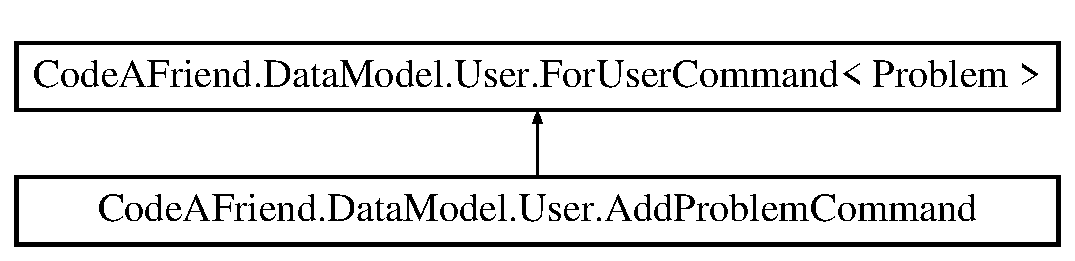
\includegraphics[height=2.000000cm]{class_code_a_friend_1_1_data_model_1_1_user_1_1_add_problem_command}
\end{center}
\end{figure}
\subsection*{Public Member Functions}
\begin{DoxyCompactItemize}
\item 
\mbox{\hyperlink{class_code_a_friend_1_1_data_model_1_1_user_1_1_add_problem_command_ab1882e37c8dc3be58d4ac74f80925407}{Add\+Problem\+Command}} (string username, string problem\+Name, string description)
\begin{DoxyCompactList}\small\item\em All properties constructor.\end{DoxyCompactList}\item 
override async Task$<$ \mbox{\hyperlink{class_code_a_friend_1_1_data_model_1_1_problem}{Problem}} $>$ \mbox{\hyperlink{class_code_a_friend_1_1_data_model_1_1_user_1_1_add_problem_command_a43eff118c9d451d384008fe68559d50d}{Execute\+Async}} (Db\+Context context)
\end{DoxyCompactItemize}
\subsection*{Properties}
\begin{DoxyCompactItemize}
\item 
string \mbox{\hyperlink{class_code_a_friend_1_1_data_model_1_1_user_1_1_add_problem_command_a6ca5b8a127f410eba3760e4959cca6f4}{Problem\+Name}}\hspace{0.3cm}{\ttfamily  \mbox{[}get, set\mbox{]}}
\begin{DoxyCompactList}\small\item\em Unique name.\end{DoxyCompactList}\item 
string \mbox{\hyperlink{class_code_a_friend_1_1_data_model_1_1_user_1_1_add_problem_command_a84d349b14a1f61a242347a617c57dbfd}{Description}}\hspace{0.3cm}{\ttfamily  \mbox{[}get, set\mbox{]}}
\begin{DoxyCompactList}\small\item\em Description of the \mbox{\hyperlink{class_code_a_friend_1_1_data_model_1_1_problem}{Problem}}.\end{DoxyCompactList}\end{DoxyCompactItemize}
\subsection*{Additional Inherited Members}


\subsection{Detailed Description}
Properties someone can specify on \mbox{\hyperlink{class_code_a_friend_1_1_data_model_1_1_problem}{Problem}} creation.



\subsection{Constructor \& Destructor Documentation}
\mbox{\Hypertarget{class_code_a_friend_1_1_data_model_1_1_user_1_1_add_problem_command_ab1882e37c8dc3be58d4ac74f80925407}\label{class_code_a_friend_1_1_data_model_1_1_user_1_1_add_problem_command_ab1882e37c8dc3be58d4ac74f80925407}} 
\index{Code\+A\+Friend\+::\+Data\+Model\+::\+User\+::\+Add\+Problem\+Command@{Code\+A\+Friend\+::\+Data\+Model\+::\+User\+::\+Add\+Problem\+Command}!Add\+Problem\+Command@{Add\+Problem\+Command}}
\index{Add\+Problem\+Command@{Add\+Problem\+Command}!Code\+A\+Friend\+::\+Data\+Model\+::\+User\+::\+Add\+Problem\+Command@{Code\+A\+Friend\+::\+Data\+Model\+::\+User\+::\+Add\+Problem\+Command}}
\subsubsection{\texorpdfstring{Add\+Problem\+Command()}{AddProblemCommand()}}
{\footnotesize\ttfamily Code\+A\+Friend.\+Data\+Model.\+User.\+Add\+Problem\+Command.\+Add\+Problem\+Command (\begin{DoxyParamCaption}\item[{string}]{username,  }\item[{string}]{problem\+Name,  }\item[{string}]{description }\end{DoxyParamCaption})}



All properties constructor.



\subsection{Member Function Documentation}
\mbox{\Hypertarget{class_code_a_friend_1_1_data_model_1_1_user_1_1_add_problem_command_a43eff118c9d451d384008fe68559d50d}\label{class_code_a_friend_1_1_data_model_1_1_user_1_1_add_problem_command_a43eff118c9d451d384008fe68559d50d}} 
\index{Code\+A\+Friend\+::\+Data\+Model\+::\+User\+::\+Add\+Problem\+Command@{Code\+A\+Friend\+::\+Data\+Model\+::\+User\+::\+Add\+Problem\+Command}!Execute\+Async@{Execute\+Async}}
\index{Execute\+Async@{Execute\+Async}!Code\+A\+Friend\+::\+Data\+Model\+::\+User\+::\+Add\+Problem\+Command@{Code\+A\+Friend\+::\+Data\+Model\+::\+User\+::\+Add\+Problem\+Command}}
\subsubsection{\texorpdfstring{Execute\+Async()}{ExecuteAsync()}}
{\footnotesize\ttfamily override async Task$<$\mbox{\hyperlink{class_code_a_friend_1_1_data_model_1_1_problem}{Problem}}$>$ Code\+A\+Friend.\+Data\+Model.\+User.\+Add\+Problem\+Command.\+Execute\+Async (\begin{DoxyParamCaption}\item[{Db\+Context}]{context }\end{DoxyParamCaption})\hspace{0.3cm}{\ttfamily [virtual]}}







Implements \mbox{\hyperlink{class_code_a_friend_1_1_data_model_1_1_user_1_1_for_user_command_aa9abf9da11dd2a573d8ed93bcf53f6df}{Code\+A\+Friend.\+Data\+Model.\+User.\+For\+User\+Command$<$ Problem $>$}}.



\subsection{Property Documentation}
\mbox{\Hypertarget{class_code_a_friend_1_1_data_model_1_1_user_1_1_add_problem_command_a84d349b14a1f61a242347a617c57dbfd}\label{class_code_a_friend_1_1_data_model_1_1_user_1_1_add_problem_command_a84d349b14a1f61a242347a617c57dbfd}} 
\index{Code\+A\+Friend\+::\+Data\+Model\+::\+User\+::\+Add\+Problem\+Command@{Code\+A\+Friend\+::\+Data\+Model\+::\+User\+::\+Add\+Problem\+Command}!Description@{Description}}
\index{Description@{Description}!Code\+A\+Friend\+::\+Data\+Model\+::\+User\+::\+Add\+Problem\+Command@{Code\+A\+Friend\+::\+Data\+Model\+::\+User\+::\+Add\+Problem\+Command}}
\subsubsection{\texorpdfstring{Description}{Description}}
{\footnotesize\ttfamily string Code\+A\+Friend.\+Data\+Model.\+User.\+Add\+Problem\+Command.\+Description\hspace{0.3cm}{\ttfamily [get]}, {\ttfamily [set]}}



Description of the \mbox{\hyperlink{class_code_a_friend_1_1_data_model_1_1_problem}{Problem}}.

\mbox{\Hypertarget{class_code_a_friend_1_1_data_model_1_1_user_1_1_add_problem_command_a6ca5b8a127f410eba3760e4959cca6f4}\label{class_code_a_friend_1_1_data_model_1_1_user_1_1_add_problem_command_a6ca5b8a127f410eba3760e4959cca6f4}} 
\index{Code\+A\+Friend\+::\+Data\+Model\+::\+User\+::\+Add\+Problem\+Command@{Code\+A\+Friend\+::\+Data\+Model\+::\+User\+::\+Add\+Problem\+Command}!Problem\+Name@{Problem\+Name}}
\index{Problem\+Name@{Problem\+Name}!Code\+A\+Friend\+::\+Data\+Model\+::\+User\+::\+Add\+Problem\+Command@{Code\+A\+Friend\+::\+Data\+Model\+::\+User\+::\+Add\+Problem\+Command}}
\subsubsection{\texorpdfstring{Problem\+Name}{ProblemName}}
{\footnotesize\ttfamily string Code\+A\+Friend.\+Data\+Model.\+User.\+Add\+Problem\+Command.\+Problem\+Name\hspace{0.3cm}{\ttfamily [get]}, {\ttfamily [set]}}



Unique name.



The documentation for this class was generated from the following file\+:\begin{DoxyCompactItemize}
\item 
shared/\+Code\+A\+Friend.\+Data\+Model/\+User\+Logic/\mbox{\hyperlink{_user_8_problem_commands_8cs}{User.\+Problem\+Commands.\+cs}}\end{DoxyCompactItemize}

\hypertarget{class_code_a_friend_1_1_data_model_1_1_user_1_1_add_script_command}{}\section{Code\+A\+Friend.\+Data\+Model.\+User.\+Add\+Script\+Command Class Reference}
\label{class_code_a_friend_1_1_data_model_1_1_user_1_1_add_script_command}\index{Code\+A\+Friend.\+Data\+Model.\+User.\+Add\+Script\+Command@{Code\+A\+Friend.\+Data\+Model.\+User.\+Add\+Script\+Command}}


Properties someone can specify on script creation. 


Inheritance diagram for Code\+A\+Friend.\+Data\+Model.\+User.\+Add\+Script\+Command\+:\begin{figure}[H]
\begin{center}
\leavevmode
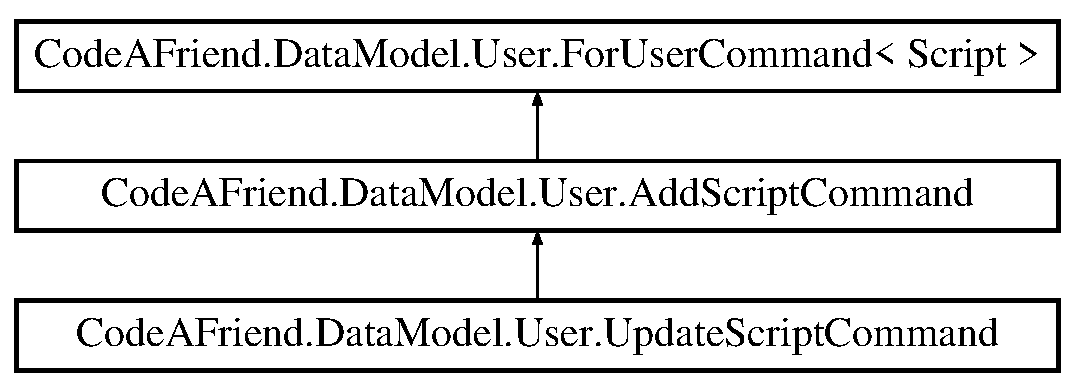
\includegraphics[height=3.000000cm]{class_code_a_friend_1_1_data_model_1_1_user_1_1_add_script_command}
\end{center}
\end{figure}
\subsection*{Public Member Functions}
\begin{DoxyCompactItemize}
\item 
\mbox{\hyperlink{class_code_a_friend_1_1_data_model_1_1_user_1_1_add_script_command_a658478472d9e31f35318e07433e85d1e}{Add\+Script\+Command}} (string username, string name, string body, \mbox{\hyperlink{namespace_code_a_friend_1_1_data_model_a13e088c525db1b03a4de75420ced79b2}{Supported\+Language}} language)
\item 
override async Task$<$ \mbox{\hyperlink{class_code_a_friend_1_1_data_model_1_1_script}{Script}} $>$ \mbox{\hyperlink{class_code_a_friend_1_1_data_model_1_1_user_1_1_add_script_command_a7105f586c7502c18a3ac2cfd567c90f0}{Execute\+Async}} (Db\+Context context)
\end{DoxyCompactItemize}
\subsection*{Properties}
\begin{DoxyCompactItemize}
\item 
string \mbox{\hyperlink{class_code_a_friend_1_1_data_model_1_1_user_1_1_add_script_command_a1863594cfd17327344a9b5d11f6ab2de}{Name}}\hspace{0.3cm}{\ttfamily  \mbox{[}get, set\mbox{]}}
\begin{DoxyCompactList}\small\item\em Name to be used to create the \mbox{\hyperlink{class_code_a_friend_1_1_data_model_1_1_script}{Script}}.\end{DoxyCompactList}\item 
string \mbox{\hyperlink{class_code_a_friend_1_1_data_model_1_1_user_1_1_add_script_command_a4c4f566ef6ce3878281ea811bd398234}{Body}}\hspace{0.3cm}{\ttfamily  \mbox{[}get, set\mbox{]}}
\begin{DoxyCompactList}\small\item\em Body of the new \mbox{\hyperlink{class_code_a_friend_1_1_data_model_1_1_script}{Script}}.\end{DoxyCompactList}\item 
\mbox{\hyperlink{namespace_code_a_friend_1_1_data_model_a13e088c525db1b03a4de75420ced79b2}{Supported\+Language}} \mbox{\hyperlink{class_code_a_friend_1_1_data_model_1_1_user_1_1_add_script_command_a9abdf5a97813615f8a7114de59ef1f40}{Language}}\hspace{0.3cm}{\ttfamily  \mbox{[}get, set\mbox{]}}
\begin{DoxyCompactList}\small\item\em Language of the new \mbox{\hyperlink{class_code_a_friend_1_1_data_model_1_1_script}{Script}}.\end{DoxyCompactList}\end{DoxyCompactItemize}
\subsection*{Additional Inherited Members}


\subsection{Detailed Description}
Properties someone can specify on script creation.



\subsection{Constructor \& Destructor Documentation}
\mbox{\Hypertarget{class_code_a_friend_1_1_data_model_1_1_user_1_1_add_script_command_a658478472d9e31f35318e07433e85d1e}\label{class_code_a_friend_1_1_data_model_1_1_user_1_1_add_script_command_a658478472d9e31f35318e07433e85d1e}} 
\index{Code\+A\+Friend\+::\+Data\+Model\+::\+User\+::\+Add\+Script\+Command@{Code\+A\+Friend\+::\+Data\+Model\+::\+User\+::\+Add\+Script\+Command}!Add\+Script\+Command@{Add\+Script\+Command}}
\index{Add\+Script\+Command@{Add\+Script\+Command}!Code\+A\+Friend\+::\+Data\+Model\+::\+User\+::\+Add\+Script\+Command@{Code\+A\+Friend\+::\+Data\+Model\+::\+User\+::\+Add\+Script\+Command}}
\subsubsection{\texorpdfstring{Add\+Script\+Command()}{AddScriptCommand()}}
{\footnotesize\ttfamily Code\+A\+Friend.\+Data\+Model.\+User.\+Add\+Script\+Command.\+Add\+Script\+Command (\begin{DoxyParamCaption}\item[{string}]{username,  }\item[{string}]{name,  }\item[{string}]{body,  }\item[{\mbox{\hyperlink{namespace_code_a_friend_1_1_data_model_a13e088c525db1b03a4de75420ced79b2}{Supported\+Language}}}]{language }\end{DoxyParamCaption})}







\subsection{Member Function Documentation}
\mbox{\Hypertarget{class_code_a_friend_1_1_data_model_1_1_user_1_1_add_script_command_a7105f586c7502c18a3ac2cfd567c90f0}\label{class_code_a_friend_1_1_data_model_1_1_user_1_1_add_script_command_a7105f586c7502c18a3ac2cfd567c90f0}} 
\index{Code\+A\+Friend\+::\+Data\+Model\+::\+User\+::\+Add\+Script\+Command@{Code\+A\+Friend\+::\+Data\+Model\+::\+User\+::\+Add\+Script\+Command}!Execute\+Async@{Execute\+Async}}
\index{Execute\+Async@{Execute\+Async}!Code\+A\+Friend\+::\+Data\+Model\+::\+User\+::\+Add\+Script\+Command@{Code\+A\+Friend\+::\+Data\+Model\+::\+User\+::\+Add\+Script\+Command}}
\subsubsection{\texorpdfstring{Execute\+Async()}{ExecuteAsync()}}
{\footnotesize\ttfamily override async Task$<$\mbox{\hyperlink{class_code_a_friend_1_1_data_model_1_1_script}{Script}}$>$ Code\+A\+Friend.\+Data\+Model.\+User.\+Add\+Script\+Command.\+Execute\+Async (\begin{DoxyParamCaption}\item[{Db\+Context}]{context }\end{DoxyParamCaption})\hspace{0.3cm}{\ttfamily [virtual]}}







Implements \mbox{\hyperlink{class_code_a_friend_1_1_data_model_1_1_user_1_1_for_user_command_aa9abf9da11dd2a573d8ed93bcf53f6df}{Code\+A\+Friend.\+Data\+Model.\+User.\+For\+User\+Command$<$ Script $>$}}.



Reimplemented in \mbox{\hyperlink{class_code_a_friend_1_1_data_model_1_1_user_1_1_update_script_command_a54e74e6d68bfc5e01cbcc96fd6dfbd2d}{Code\+A\+Friend.\+Data\+Model.\+User.\+Update\+Script\+Command}}.



\subsection{Property Documentation}
\mbox{\Hypertarget{class_code_a_friend_1_1_data_model_1_1_user_1_1_add_script_command_a4c4f566ef6ce3878281ea811bd398234}\label{class_code_a_friend_1_1_data_model_1_1_user_1_1_add_script_command_a4c4f566ef6ce3878281ea811bd398234}} 
\index{Code\+A\+Friend\+::\+Data\+Model\+::\+User\+::\+Add\+Script\+Command@{Code\+A\+Friend\+::\+Data\+Model\+::\+User\+::\+Add\+Script\+Command}!Body@{Body}}
\index{Body@{Body}!Code\+A\+Friend\+::\+Data\+Model\+::\+User\+::\+Add\+Script\+Command@{Code\+A\+Friend\+::\+Data\+Model\+::\+User\+::\+Add\+Script\+Command}}
\subsubsection{\texorpdfstring{Body}{Body}}
{\footnotesize\ttfamily string Code\+A\+Friend.\+Data\+Model.\+User.\+Add\+Script\+Command.\+Body\hspace{0.3cm}{\ttfamily [get]}, {\ttfamily [set]}}



Body of the new \mbox{\hyperlink{class_code_a_friend_1_1_data_model_1_1_script}{Script}}.

\mbox{\Hypertarget{class_code_a_friend_1_1_data_model_1_1_user_1_1_add_script_command_a9abdf5a97813615f8a7114de59ef1f40}\label{class_code_a_friend_1_1_data_model_1_1_user_1_1_add_script_command_a9abdf5a97813615f8a7114de59ef1f40}} 
\index{Code\+A\+Friend\+::\+Data\+Model\+::\+User\+::\+Add\+Script\+Command@{Code\+A\+Friend\+::\+Data\+Model\+::\+User\+::\+Add\+Script\+Command}!Language@{Language}}
\index{Language@{Language}!Code\+A\+Friend\+::\+Data\+Model\+::\+User\+::\+Add\+Script\+Command@{Code\+A\+Friend\+::\+Data\+Model\+::\+User\+::\+Add\+Script\+Command}}
\subsubsection{\texorpdfstring{Language}{Language}}
{\footnotesize\ttfamily \mbox{\hyperlink{namespace_code_a_friend_1_1_data_model_a13e088c525db1b03a4de75420ced79b2}{Supported\+Language}} Code\+A\+Friend.\+Data\+Model.\+User.\+Add\+Script\+Command.\+Language\hspace{0.3cm}{\ttfamily [get]}, {\ttfamily [set]}}



Language of the new \mbox{\hyperlink{class_code_a_friend_1_1_data_model_1_1_script}{Script}}.

\mbox{\Hypertarget{class_code_a_friend_1_1_data_model_1_1_user_1_1_add_script_command_a1863594cfd17327344a9b5d11f6ab2de}\label{class_code_a_friend_1_1_data_model_1_1_user_1_1_add_script_command_a1863594cfd17327344a9b5d11f6ab2de}} 
\index{Code\+A\+Friend\+::\+Data\+Model\+::\+User\+::\+Add\+Script\+Command@{Code\+A\+Friend\+::\+Data\+Model\+::\+User\+::\+Add\+Script\+Command}!Name@{Name}}
\index{Name@{Name}!Code\+A\+Friend\+::\+Data\+Model\+::\+User\+::\+Add\+Script\+Command@{Code\+A\+Friend\+::\+Data\+Model\+::\+User\+::\+Add\+Script\+Command}}
\subsubsection{\texorpdfstring{Name}{Name}}
{\footnotesize\ttfamily string Code\+A\+Friend.\+Data\+Model.\+User.\+Add\+Script\+Command.\+Name\hspace{0.3cm}{\ttfamily [get]}, {\ttfamily [set]}}



Name to be used to create the \mbox{\hyperlink{class_code_a_friend_1_1_data_model_1_1_script}{Script}}.



The documentation for this class was generated from the following file\+:\begin{DoxyCompactItemize}
\item 
shared/\+Code\+A\+Friend.\+Data\+Model/\+User\+Logic/\mbox{\hyperlink{_user_8_script_commands_8cs}{User.\+Script\+Commands.\+cs}}\end{DoxyCompactItemize}

\hypertarget{class_code_a_friend_1_1_api_service_1_1_controllers_1_1_coda_a_friend_controller}{}\section{Code\+A\+Friend.\+Api\+Service.\+Controllers.\+Coda\+A\+Friend\+Controller Class Reference}
\label{class_code_a_friend_1_1_api_service_1_1_controllers_1_1_coda_a_friend_controller}\index{Code\+A\+Friend.\+Api\+Service.\+Controllers.\+Coda\+A\+Friend\+Controller@{Code\+A\+Friend.\+Api\+Service.\+Controllers.\+Coda\+A\+Friend\+Controller}}


Set of Api methods for manipulating Cod\+A\+Friend objects.  


Inheritance diagram for Code\+A\+Friend.\+Api\+Service.\+Controllers.\+Coda\+A\+Friend\+Controller\+:\begin{figure}[H]
\begin{center}
\leavevmode
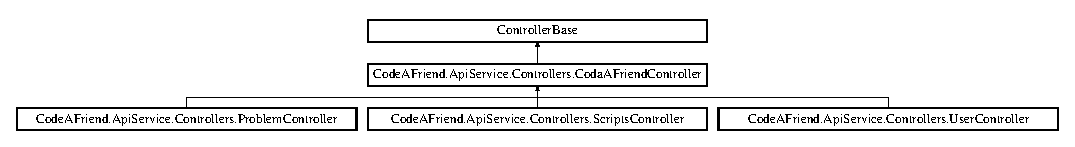
\includegraphics[height=1.534247cm]{class_code_a_friend_1_1_api_service_1_1_controllers_1_1_coda_a_friend_controller}
\end{center}
\end{figure}
\subsection*{Protected Member Functions}
\begin{DoxyCompactItemize}
\item 
\mbox{\hyperlink{class_code_a_friend_1_1_api_service_1_1_controllers_1_1_coda_a_friend_controller_ab39f44a0cbe572d4e3a7a94634b2c199}{Coda\+A\+Friend\+Controller}} (\mbox{\hyperlink{interface_code_a_friend_1_1_facade_1_1_i_code_a_friend_facade}{I\+Code\+A\+Friend\+Facade}} facade)
\begin{DoxyCompactList}\small\item\em DI constructor. \end{DoxyCompactList}\end{DoxyCompactItemize}
\subsection*{Protected Attributes}
\begin{DoxyCompactItemize}
\item 
\mbox{\hyperlink{interface_code_a_friend_1_1_facade_1_1_i_code_a_friend_facade}{I\+Code\+A\+Friend\+Facade}} \mbox{\hyperlink{class_code_a_friend_1_1_api_service_1_1_controllers_1_1_coda_a_friend_controller_a5a9aff99d4e9ba347547fc3a5ae26b18}{Facade}}
\begin{DoxyCompactList}\small\item\em I\+Code\+A\+Friend\+Facade where all Cod\+A\+Friend objects are stored. \end{DoxyCompactList}\end{DoxyCompactItemize}


\subsection{Detailed Description}
Set of Api methods for manipulating Cod\+A\+Friend objects. 



\subsection{Constructor \& Destructor Documentation}
\mbox{\Hypertarget{class_code_a_friend_1_1_api_service_1_1_controllers_1_1_coda_a_friend_controller_ab39f44a0cbe572d4e3a7a94634b2c199}\label{class_code_a_friend_1_1_api_service_1_1_controllers_1_1_coda_a_friend_controller_ab39f44a0cbe572d4e3a7a94634b2c199}} 
\index{Code\+A\+Friend\+::\+Api\+Service\+::\+Controllers\+::\+Coda\+A\+Friend\+Controller@{Code\+A\+Friend\+::\+Api\+Service\+::\+Controllers\+::\+Coda\+A\+Friend\+Controller}!Coda\+A\+Friend\+Controller@{Coda\+A\+Friend\+Controller}}
\index{Coda\+A\+Friend\+Controller@{Coda\+A\+Friend\+Controller}!Code\+A\+Friend\+::\+Api\+Service\+::\+Controllers\+::\+Coda\+A\+Friend\+Controller@{Code\+A\+Friend\+::\+Api\+Service\+::\+Controllers\+::\+Coda\+A\+Friend\+Controller}}
\subsubsection{\texorpdfstring{Coda\+A\+Friend\+Controller()}{CodaAFriendController()}}
{\footnotesize\ttfamily Code\+A\+Friend.\+Api\+Service.\+Controllers.\+Coda\+A\+Friend\+Controller.\+Coda\+A\+Friend\+Controller (\begin{DoxyParamCaption}\item[{\mbox{\hyperlink{interface_code_a_friend_1_1_facade_1_1_i_code_a_friend_facade}{I\+Code\+A\+Friend\+Facade}}}]{facade }\end{DoxyParamCaption})\hspace{0.3cm}{\ttfamily [protected]}}



DI constructor. 



\subsection{Member Data Documentation}
\mbox{\Hypertarget{class_code_a_friend_1_1_api_service_1_1_controllers_1_1_coda_a_friend_controller_a5a9aff99d4e9ba347547fc3a5ae26b18}\label{class_code_a_friend_1_1_api_service_1_1_controllers_1_1_coda_a_friend_controller_a5a9aff99d4e9ba347547fc3a5ae26b18}} 
\index{Code\+A\+Friend\+::\+Api\+Service\+::\+Controllers\+::\+Coda\+A\+Friend\+Controller@{Code\+A\+Friend\+::\+Api\+Service\+::\+Controllers\+::\+Coda\+A\+Friend\+Controller}!Facade@{Facade}}
\index{Facade@{Facade}!Code\+A\+Friend\+::\+Api\+Service\+::\+Controllers\+::\+Coda\+A\+Friend\+Controller@{Code\+A\+Friend\+::\+Api\+Service\+::\+Controllers\+::\+Coda\+A\+Friend\+Controller}}
\subsubsection{\texorpdfstring{Facade}{Facade}}
{\footnotesize\ttfamily \mbox{\hyperlink{interface_code_a_friend_1_1_facade_1_1_i_code_a_friend_facade}{I\+Code\+A\+Friend\+Facade}} Code\+A\+Friend.\+Api\+Service.\+Controllers.\+Coda\+A\+Friend\+Controller.\+Facade\hspace{0.3cm}{\ttfamily [protected]}}



I\+Code\+A\+Friend\+Facade where all Cod\+A\+Friend objects are stored. 



The documentation for this class was generated from the following file\+:\begin{DoxyCompactItemize}
\item 
apps/\+Code\+A\+Friend.\+Api\+Service/\+Controllers/\mbox{\hyperlink{_coda_a_friend_controller_8cs}{Coda\+A\+Friend\+Controller.\+cs}}\end{DoxyCompactItemize}

\hypertarget{class_code_a_friend_1_1_repository_1_1_code_a_friend_context}{}\section{Code\+A\+Friend.\+Repository.\+Code\+A\+Friend\+Context Class Reference}
\label{class_code_a_friend_1_1_repository_1_1_code_a_friend_context}\index{Code\+A\+Friend.\+Repository.\+Code\+A\+Friend\+Context@{Code\+A\+Friend.\+Repository.\+Code\+A\+Friend\+Context}}


EF \mbox{\hyperlink{namespace_code_a_friend_1_1_core}{Core}} object used to configure and access stored business objects in the \mbox{\hyperlink{namespace_code_a_friend}{Code\+A\+Friend}} system. 


Inheritance diagram for Code\+A\+Friend.\+Repository.\+Code\+A\+Friend\+Context\+:\begin{figure}[H]
\begin{center}
\leavevmode
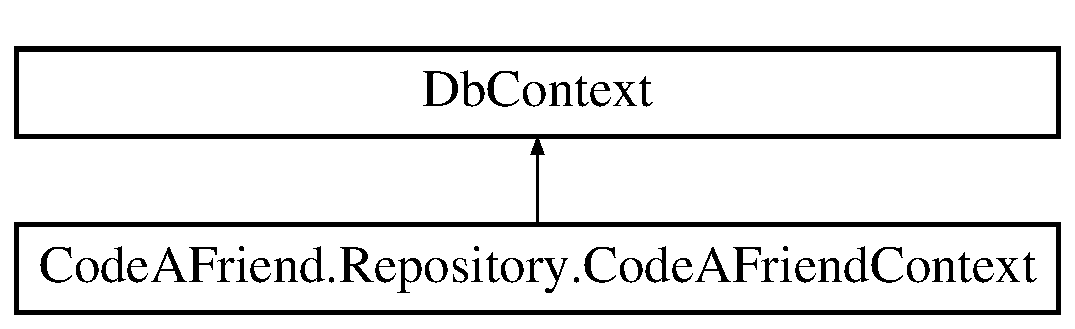
\includegraphics[height=2.000000cm]{class_code_a_friend_1_1_repository_1_1_code_a_friend_context}
\end{center}
\end{figure}
\subsection*{Public Member Functions}
\begin{DoxyCompactItemize}
\item 
\mbox{\hyperlink{class_code_a_friend_1_1_repository_1_1_code_a_friend_context_a76820d5c0525ba70dbf679fe5bc3a744}{Code\+A\+Friend\+Context}} ()
\item 
\mbox{\hyperlink{class_code_a_friend_1_1_repository_1_1_code_a_friend_context_a48086a6d09a4cd0604f5aaf4a0c7a220}{Code\+A\+Friend\+Context}} (Db\+Context\+Options$<$ \mbox{\hyperlink{class_code_a_friend_1_1_repository_1_1_code_a_friend_context}{Code\+A\+Friend\+Context}} $>$ options)
\end{DoxyCompactItemize}
\subsection*{Protected Member Functions}
\begin{DoxyCompactItemize}
\item 
override void \mbox{\hyperlink{class_code_a_friend_1_1_repository_1_1_code_a_friend_context_a7465fc81cf21b6bf649a5265aea7c454}{On\+Configuring}} (Db\+Context\+Options\+Builder options\+Builder)
\item 
override void \mbox{\hyperlink{class_code_a_friend_1_1_repository_1_1_code_a_friend_context_aede2ea79950908629468b17b4a53ec04}{On\+Model\+Creating}} (Model\+Builder model\+Builder)
\end{DoxyCompactItemize}
\subsection*{Properties}
\begin{DoxyCompactItemize}
\item 
Db\+Set$<$ \mbox{\hyperlink{class_code_a_friend_1_1_data_model_1_1_problem}{Problem}} $>$ \mbox{\hyperlink{class_code_a_friend_1_1_repository_1_1_code_a_friend_context_a29c223337459ca32c2831de84993b73d}{Problems}}\hspace{0.3cm}{\ttfamily  \mbox{[}get, set\mbox{]}}
\begin{DoxyCompactList}\small\item\em Table that holds Problems.\end{DoxyCompactList}\item 
Db\+Set$<$ \mbox{\hyperlink{class_code_a_friend_1_1_data_model_1_1_problem_solution}{Problem\+Solution}} $>$ \mbox{\hyperlink{class_code_a_friend_1_1_repository_1_1_code_a_friend_context_a58b681af6a297c85487e2454ef51ac01}{Problem\+Solutions}}\hspace{0.3cm}{\ttfamily  \mbox{[}get, set\mbox{]}}
\begin{DoxyCompactList}\small\item\em Table that holds Problem Solutions.\end{DoxyCompactList}\item 
Db\+Set$<$ \mbox{\hyperlink{class_code_a_friend_1_1_data_model_1_1_vote}{Vote}} $>$ \mbox{\hyperlink{class_code_a_friend_1_1_repository_1_1_code_a_friend_context_a51510b18f90a485162292c9674df33a3}{Problem\+Solution\+Votes}}\hspace{0.3cm}{\ttfamily  \mbox{[}get, set\mbox{]}}
\begin{DoxyCompactList}\small\item\em Table that holds Problem Solutions.\end{DoxyCompactList}\item 
Db\+Set$<$ \mbox{\hyperlink{class_code_a_friend_1_1_data_model_1_1_test_case}{Test\+Case}} $>$ \mbox{\hyperlink{class_code_a_friend_1_1_repository_1_1_code_a_friend_context_a67843b6a9a6180107c1721b671d029a4}{Problem\+Test\+Cases}}\hspace{0.3cm}{\ttfamily  \mbox{[}get, set\mbox{]}}
\begin{DoxyCompactList}\small\item\em Table that holds Problem Test\+Cases.\end{DoxyCompactList}\item 
Db\+Set$<$ \mbox{\hyperlink{class_code_a_friend_1_1_data_model_1_1_tag}{Tag}} $>$ \mbox{\hyperlink{class_code_a_friend_1_1_repository_1_1_code_a_friend_context_a79eb1ed9a0502b24bb0c4832f5333495}{Problem\+Tags}}\hspace{0.3cm}{\ttfamily  \mbox{[}get, set\mbox{]}}
\begin{DoxyCompactList}\small\item\em Table that holds Problem Tags.\end{DoxyCompactList}\item 
Db\+Set$<$ \mbox{\hyperlink{class_code_a_friend_1_1_data_model_1_1_user}{User}} $>$ \mbox{\hyperlink{class_code_a_friend_1_1_repository_1_1_code_a_friend_context_aa4b0cd6d707e8e05e6dbac7fa6b225b9}{Users}}\hspace{0.3cm}{\ttfamily  \mbox{[}get, set\mbox{]}}
\begin{DoxyCompactList}\small\item\em Table that holds Users.\end{DoxyCompactList}\item 
Db\+Set$<$ \mbox{\hyperlink{class_code_a_friend_1_1_data_model_1_1_user_script}{User\+Script}} $>$ \mbox{\hyperlink{class_code_a_friend_1_1_repository_1_1_code_a_friend_context_aa2d9d4f6cf003b7ee1364c954ee3fad5}{User\+Scripts}}\hspace{0.3cm}{\ttfamily  \mbox{[}get, set\mbox{]}}
\begin{DoxyCompactList}\small\item\em Table that holds User Scripts.\end{DoxyCompactList}\end{DoxyCompactItemize}


\subsection{Detailed Description}
EF \mbox{\hyperlink{namespace_code_a_friend_1_1_core}{Core}} object used to configure and access stored business objects in the \mbox{\hyperlink{namespace_code_a_friend}{Code\+A\+Friend}} system.



\subsection{Constructor \& Destructor Documentation}
\mbox{\Hypertarget{class_code_a_friend_1_1_repository_1_1_code_a_friend_context_a76820d5c0525ba70dbf679fe5bc3a744}\label{class_code_a_friend_1_1_repository_1_1_code_a_friend_context_a76820d5c0525ba70dbf679fe5bc3a744}} 
\index{Code\+A\+Friend\+::\+Repository\+::\+Code\+A\+Friend\+Context@{Code\+A\+Friend\+::\+Repository\+::\+Code\+A\+Friend\+Context}!Code\+A\+Friend\+Context@{Code\+A\+Friend\+Context}}
\index{Code\+A\+Friend\+Context@{Code\+A\+Friend\+Context}!Code\+A\+Friend\+::\+Repository\+::\+Code\+A\+Friend\+Context@{Code\+A\+Friend\+::\+Repository\+::\+Code\+A\+Friend\+Context}}
\subsubsection{\texorpdfstring{Code\+A\+Friend\+Context()}{CodeAFriendContext()}\hspace{0.1cm}{\footnotesize\ttfamily [1/2]}}
{\footnotesize\ttfamily Code\+A\+Friend.\+Repository.\+Code\+A\+Friend\+Context.\+Code\+A\+Friend\+Context (\begin{DoxyParamCaption}{ }\end{DoxyParamCaption})}





\mbox{\Hypertarget{class_code_a_friend_1_1_repository_1_1_code_a_friend_context_a48086a6d09a4cd0604f5aaf4a0c7a220}\label{class_code_a_friend_1_1_repository_1_1_code_a_friend_context_a48086a6d09a4cd0604f5aaf4a0c7a220}} 
\index{Code\+A\+Friend\+::\+Repository\+::\+Code\+A\+Friend\+Context@{Code\+A\+Friend\+::\+Repository\+::\+Code\+A\+Friend\+Context}!Code\+A\+Friend\+Context@{Code\+A\+Friend\+Context}}
\index{Code\+A\+Friend\+Context@{Code\+A\+Friend\+Context}!Code\+A\+Friend\+::\+Repository\+::\+Code\+A\+Friend\+Context@{Code\+A\+Friend\+::\+Repository\+::\+Code\+A\+Friend\+Context}}
\subsubsection{\texorpdfstring{Code\+A\+Friend\+Context()}{CodeAFriendContext()}\hspace{0.1cm}{\footnotesize\ttfamily [2/2]}}
{\footnotesize\ttfamily Code\+A\+Friend.\+Repository.\+Code\+A\+Friend\+Context.\+Code\+A\+Friend\+Context (\begin{DoxyParamCaption}\item[{Db\+Context\+Options$<$ \mbox{\hyperlink{class_code_a_friend_1_1_repository_1_1_code_a_friend_context}{Code\+A\+Friend\+Context}} $>$}]{options }\end{DoxyParamCaption})}







\subsection{Member Function Documentation}
\mbox{\Hypertarget{class_code_a_friend_1_1_repository_1_1_code_a_friend_context_a7465fc81cf21b6bf649a5265aea7c454}\label{class_code_a_friend_1_1_repository_1_1_code_a_friend_context_a7465fc81cf21b6bf649a5265aea7c454}} 
\index{Code\+A\+Friend\+::\+Repository\+::\+Code\+A\+Friend\+Context@{Code\+A\+Friend\+::\+Repository\+::\+Code\+A\+Friend\+Context}!On\+Configuring@{On\+Configuring}}
\index{On\+Configuring@{On\+Configuring}!Code\+A\+Friend\+::\+Repository\+::\+Code\+A\+Friend\+Context@{Code\+A\+Friend\+::\+Repository\+::\+Code\+A\+Friend\+Context}}
\subsubsection{\texorpdfstring{On\+Configuring()}{OnConfiguring()}}
{\footnotesize\ttfamily override void Code\+A\+Friend.\+Repository.\+Code\+A\+Friend\+Context.\+On\+Configuring (\begin{DoxyParamCaption}\item[{Db\+Context\+Options\+Builder}]{options\+Builder }\end{DoxyParamCaption})\hspace{0.3cm}{\ttfamily [protected]}}





\mbox{\Hypertarget{class_code_a_friend_1_1_repository_1_1_code_a_friend_context_aede2ea79950908629468b17b4a53ec04}\label{class_code_a_friend_1_1_repository_1_1_code_a_friend_context_aede2ea79950908629468b17b4a53ec04}} 
\index{Code\+A\+Friend\+::\+Repository\+::\+Code\+A\+Friend\+Context@{Code\+A\+Friend\+::\+Repository\+::\+Code\+A\+Friend\+Context}!On\+Model\+Creating@{On\+Model\+Creating}}
\index{On\+Model\+Creating@{On\+Model\+Creating}!Code\+A\+Friend\+::\+Repository\+::\+Code\+A\+Friend\+Context@{Code\+A\+Friend\+::\+Repository\+::\+Code\+A\+Friend\+Context}}
\subsubsection{\texorpdfstring{On\+Model\+Creating()}{OnModelCreating()}}
{\footnotesize\ttfamily override void Code\+A\+Friend.\+Repository.\+Code\+A\+Friend\+Context.\+On\+Model\+Creating (\begin{DoxyParamCaption}\item[{Model\+Builder}]{model\+Builder }\end{DoxyParamCaption})\hspace{0.3cm}{\ttfamily [protected]}}







\subsection{Property Documentation}
\mbox{\Hypertarget{class_code_a_friend_1_1_repository_1_1_code_a_friend_context_a29c223337459ca32c2831de84993b73d}\label{class_code_a_friend_1_1_repository_1_1_code_a_friend_context_a29c223337459ca32c2831de84993b73d}} 
\index{Code\+A\+Friend\+::\+Repository\+::\+Code\+A\+Friend\+Context@{Code\+A\+Friend\+::\+Repository\+::\+Code\+A\+Friend\+Context}!Problems@{Problems}}
\index{Problems@{Problems}!Code\+A\+Friend\+::\+Repository\+::\+Code\+A\+Friend\+Context@{Code\+A\+Friend\+::\+Repository\+::\+Code\+A\+Friend\+Context}}
\subsubsection{\texorpdfstring{Problems}{Problems}}
{\footnotesize\ttfamily Db\+Set$<$\mbox{\hyperlink{class_code_a_friend_1_1_data_model_1_1_problem}{Problem}}$>$ Code\+A\+Friend.\+Repository.\+Code\+A\+Friend\+Context.\+Problems\hspace{0.3cm}{\ttfamily [get]}, {\ttfamily [set]}}



Table that holds Problems.

\mbox{\Hypertarget{class_code_a_friend_1_1_repository_1_1_code_a_friend_context_a58b681af6a297c85487e2454ef51ac01}\label{class_code_a_friend_1_1_repository_1_1_code_a_friend_context_a58b681af6a297c85487e2454ef51ac01}} 
\index{Code\+A\+Friend\+::\+Repository\+::\+Code\+A\+Friend\+Context@{Code\+A\+Friend\+::\+Repository\+::\+Code\+A\+Friend\+Context}!Problem\+Solutions@{Problem\+Solutions}}
\index{Problem\+Solutions@{Problem\+Solutions}!Code\+A\+Friend\+::\+Repository\+::\+Code\+A\+Friend\+Context@{Code\+A\+Friend\+::\+Repository\+::\+Code\+A\+Friend\+Context}}
\subsubsection{\texorpdfstring{Problem\+Solutions}{ProblemSolutions}}
{\footnotesize\ttfamily Db\+Set$<$\mbox{\hyperlink{class_code_a_friend_1_1_data_model_1_1_problem_solution}{Problem\+Solution}}$>$ Code\+A\+Friend.\+Repository.\+Code\+A\+Friend\+Context.\+Problem\+Solutions\hspace{0.3cm}{\ttfamily [get]}, {\ttfamily [set]}}



Table that holds Problem Solutions.

\mbox{\Hypertarget{class_code_a_friend_1_1_repository_1_1_code_a_friend_context_a51510b18f90a485162292c9674df33a3}\label{class_code_a_friend_1_1_repository_1_1_code_a_friend_context_a51510b18f90a485162292c9674df33a3}} 
\index{Code\+A\+Friend\+::\+Repository\+::\+Code\+A\+Friend\+Context@{Code\+A\+Friend\+::\+Repository\+::\+Code\+A\+Friend\+Context}!Problem\+Solution\+Votes@{Problem\+Solution\+Votes}}
\index{Problem\+Solution\+Votes@{Problem\+Solution\+Votes}!Code\+A\+Friend\+::\+Repository\+::\+Code\+A\+Friend\+Context@{Code\+A\+Friend\+::\+Repository\+::\+Code\+A\+Friend\+Context}}
\subsubsection{\texorpdfstring{Problem\+Solution\+Votes}{ProblemSolutionVotes}}
{\footnotesize\ttfamily Db\+Set$<$\mbox{\hyperlink{class_code_a_friend_1_1_data_model_1_1_vote}{Vote}}$>$ Code\+A\+Friend.\+Repository.\+Code\+A\+Friend\+Context.\+Problem\+Solution\+Votes\hspace{0.3cm}{\ttfamily [get]}, {\ttfamily [set]}}



Table that holds Problem Solutions.

\mbox{\Hypertarget{class_code_a_friend_1_1_repository_1_1_code_a_friend_context_a79eb1ed9a0502b24bb0c4832f5333495}\label{class_code_a_friend_1_1_repository_1_1_code_a_friend_context_a79eb1ed9a0502b24bb0c4832f5333495}} 
\index{Code\+A\+Friend\+::\+Repository\+::\+Code\+A\+Friend\+Context@{Code\+A\+Friend\+::\+Repository\+::\+Code\+A\+Friend\+Context}!Problem\+Tags@{Problem\+Tags}}
\index{Problem\+Tags@{Problem\+Tags}!Code\+A\+Friend\+::\+Repository\+::\+Code\+A\+Friend\+Context@{Code\+A\+Friend\+::\+Repository\+::\+Code\+A\+Friend\+Context}}
\subsubsection{\texorpdfstring{Problem\+Tags}{ProblemTags}}
{\footnotesize\ttfamily Db\+Set$<$\mbox{\hyperlink{class_code_a_friend_1_1_data_model_1_1_tag}{Tag}}$>$ Code\+A\+Friend.\+Repository.\+Code\+A\+Friend\+Context.\+Problem\+Tags\hspace{0.3cm}{\ttfamily [get]}, {\ttfamily [set]}}



Table that holds Problem Tags.

\mbox{\Hypertarget{class_code_a_friend_1_1_repository_1_1_code_a_friend_context_a67843b6a9a6180107c1721b671d029a4}\label{class_code_a_friend_1_1_repository_1_1_code_a_friend_context_a67843b6a9a6180107c1721b671d029a4}} 
\index{Code\+A\+Friend\+::\+Repository\+::\+Code\+A\+Friend\+Context@{Code\+A\+Friend\+::\+Repository\+::\+Code\+A\+Friend\+Context}!Problem\+Test\+Cases@{Problem\+Test\+Cases}}
\index{Problem\+Test\+Cases@{Problem\+Test\+Cases}!Code\+A\+Friend\+::\+Repository\+::\+Code\+A\+Friend\+Context@{Code\+A\+Friend\+::\+Repository\+::\+Code\+A\+Friend\+Context}}
\subsubsection{\texorpdfstring{Problem\+Test\+Cases}{ProblemTestCases}}
{\footnotesize\ttfamily Db\+Set$<$\mbox{\hyperlink{class_code_a_friend_1_1_data_model_1_1_test_case}{Test\+Case}}$>$ Code\+A\+Friend.\+Repository.\+Code\+A\+Friend\+Context.\+Problem\+Test\+Cases\hspace{0.3cm}{\ttfamily [get]}, {\ttfamily [set]}}



Table that holds Problem Test\+Cases.

\mbox{\Hypertarget{class_code_a_friend_1_1_repository_1_1_code_a_friend_context_aa4b0cd6d707e8e05e6dbac7fa6b225b9}\label{class_code_a_friend_1_1_repository_1_1_code_a_friend_context_aa4b0cd6d707e8e05e6dbac7fa6b225b9}} 
\index{Code\+A\+Friend\+::\+Repository\+::\+Code\+A\+Friend\+Context@{Code\+A\+Friend\+::\+Repository\+::\+Code\+A\+Friend\+Context}!Users@{Users}}
\index{Users@{Users}!Code\+A\+Friend\+::\+Repository\+::\+Code\+A\+Friend\+Context@{Code\+A\+Friend\+::\+Repository\+::\+Code\+A\+Friend\+Context}}
\subsubsection{\texorpdfstring{Users}{Users}}
{\footnotesize\ttfamily Db\+Set$<$\mbox{\hyperlink{class_code_a_friend_1_1_data_model_1_1_user}{User}}$>$ Code\+A\+Friend.\+Repository.\+Code\+A\+Friend\+Context.\+Users\hspace{0.3cm}{\ttfamily [get]}, {\ttfamily [set]}}



Table that holds Users.

\mbox{\Hypertarget{class_code_a_friend_1_1_repository_1_1_code_a_friend_context_aa2d9d4f6cf003b7ee1364c954ee3fad5}\label{class_code_a_friend_1_1_repository_1_1_code_a_friend_context_aa2d9d4f6cf003b7ee1364c954ee3fad5}} 
\index{Code\+A\+Friend\+::\+Repository\+::\+Code\+A\+Friend\+Context@{Code\+A\+Friend\+::\+Repository\+::\+Code\+A\+Friend\+Context}!User\+Scripts@{User\+Scripts}}
\index{User\+Scripts@{User\+Scripts}!Code\+A\+Friend\+::\+Repository\+::\+Code\+A\+Friend\+Context@{Code\+A\+Friend\+::\+Repository\+::\+Code\+A\+Friend\+Context}}
\subsubsection{\texorpdfstring{User\+Scripts}{UserScripts}}
{\footnotesize\ttfamily Db\+Set$<$\mbox{\hyperlink{class_code_a_friend_1_1_data_model_1_1_user_script}{User\+Script}}$>$ Code\+A\+Friend.\+Repository.\+Code\+A\+Friend\+Context.\+User\+Scripts\hspace{0.3cm}{\ttfamily [get]}, {\ttfamily [set]}}



Table that holds User Scripts.



The documentation for this class was generated from the following file\+:\begin{DoxyCompactItemize}
\item 
shared/\+Code\+A\+Friend.\+Repository/\mbox{\hyperlink{_code_a_friend_context_8cs}{Code\+A\+Friend\+Context.\+cs}}\end{DoxyCompactItemize}

\hypertarget{class_code_a_friend_1_1_repository_1_1_migrations_1_1_code_a_friend_context_model_snapshot}{}\section{Code\+A\+Friend.\+Repository.\+Migrations.\+Code\+A\+Friend\+Context\+Model\+Snapshot Class Reference}
\label{class_code_a_friend_1_1_repository_1_1_migrations_1_1_code_a_friend_context_model_snapshot}\index{Code\+A\+Friend.\+Repository.\+Migrations.\+Code\+A\+Friend\+Context\+Model\+Snapshot@{Code\+A\+Friend.\+Repository.\+Migrations.\+Code\+A\+Friend\+Context\+Model\+Snapshot}}
Inheritance diagram for Code\+A\+Friend.\+Repository.\+Migrations.\+Code\+A\+Friend\+Context\+Model\+Snapshot\+:\begin{figure}[H]
\begin{center}
\leavevmode
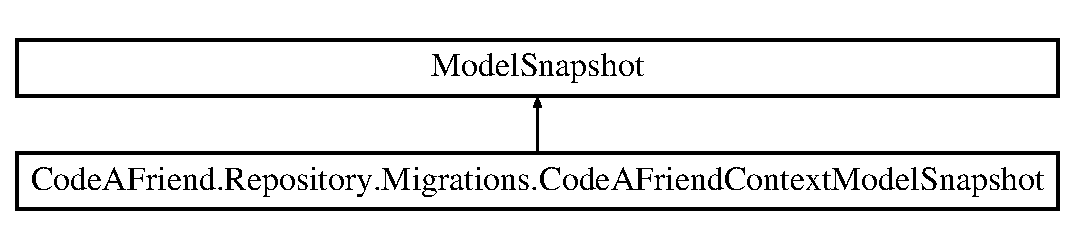
\includegraphics[height=2.000000cm]{class_code_a_friend_1_1_repository_1_1_migrations_1_1_code_a_friend_context_model_snapshot}
\end{center}
\end{figure}
\subsection*{Protected Member Functions}
\begin{DoxyCompactItemize}
\item 
override void \mbox{\hyperlink{class_code_a_friend_1_1_repository_1_1_migrations_1_1_code_a_friend_context_model_snapshot_a1155a6c780f4d8fc273bb168999f8cd6}{Build\+Model}} (Model\+Builder model\+Builder)
\end{DoxyCompactItemize}


\subsection{Member Function Documentation}
\mbox{\Hypertarget{class_code_a_friend_1_1_repository_1_1_migrations_1_1_code_a_friend_context_model_snapshot_a1155a6c780f4d8fc273bb168999f8cd6}\label{class_code_a_friend_1_1_repository_1_1_migrations_1_1_code_a_friend_context_model_snapshot_a1155a6c780f4d8fc273bb168999f8cd6}} 
\index{Code\+A\+Friend\+::\+Repository\+::\+Migrations\+::\+Code\+A\+Friend\+Context\+Model\+Snapshot@{Code\+A\+Friend\+::\+Repository\+::\+Migrations\+::\+Code\+A\+Friend\+Context\+Model\+Snapshot}!Build\+Model@{Build\+Model}}
\index{Build\+Model@{Build\+Model}!Code\+A\+Friend\+::\+Repository\+::\+Migrations\+::\+Code\+A\+Friend\+Context\+Model\+Snapshot@{Code\+A\+Friend\+::\+Repository\+::\+Migrations\+::\+Code\+A\+Friend\+Context\+Model\+Snapshot}}
\subsubsection{\texorpdfstring{Build\+Model()}{BuildModel()}}
{\footnotesize\ttfamily override void Code\+A\+Friend.\+Repository.\+Migrations.\+Code\+A\+Friend\+Context\+Model\+Snapshot.\+Build\+Model (\begin{DoxyParamCaption}\item[{Model\+Builder}]{model\+Builder }\end{DoxyParamCaption})\hspace{0.3cm}{\ttfamily [protected]}}



The documentation for this class was generated from the following file\+:\begin{DoxyCompactItemize}
\item 
shared/\+Code\+A\+Friend.\+Repository/\+Migrations/\mbox{\hyperlink{_code_a_friend_context_model_snapshot_8cs}{Code\+A\+Friend\+Context\+Model\+Snapshot.\+cs}}\end{DoxyCompactItemize}

\hypertarget{class_code_a_friend_1_1_facade_1_1_code_a_friend_facade}{}\section{Code\+A\+Friend.\+Facade.\+Code\+A\+Friend\+Facade Class Reference}
\label{class_code_a_friend_1_1_facade_1_1_code_a_friend_facade}\index{Code\+A\+Friend.\+Facade.\+Code\+A\+Friend\+Facade@{Code\+A\+Friend.\+Facade.\+Code\+A\+Friend\+Facade}}


 


Inheritance diagram for Code\+A\+Friend.\+Facade.\+Code\+A\+Friend\+Facade\+:\begin{figure}[H]
\begin{center}
\leavevmode
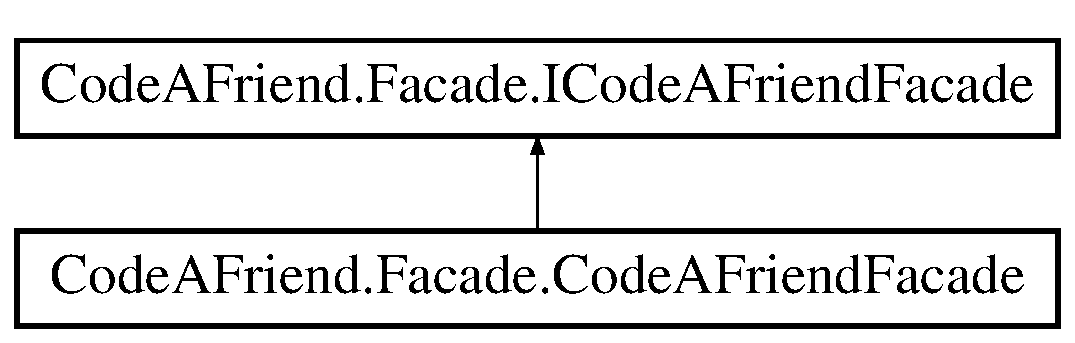
\includegraphics[height=2.000000cm]{class_code_a_friend_1_1_facade_1_1_code_a_friend_facade}
\end{center}
\end{figure}
\subsection*{Public Member Functions}
\begin{DoxyCompactItemize}
\item 
\mbox{\hyperlink{class_code_a_friend_1_1_facade_1_1_code_a_friend_facade_a97f88a6ad57d442f503cbd0aa3de95ae}{Code\+A\+Friend\+Facade}} (Db\+Context db\+Context, \mbox{\hyperlink{interface_code_a_friend_1_1_languages_1_1_core_1_1_i_interpreter_factory}{I\+Interpreter\+Factory}} interpreter\+Factory)
\begin{DoxyCompactList}\small\item\em DI Constructor\end{DoxyCompactList}\item 
async Task$<$ T\+Result $>$ \mbox{\hyperlink{class_code_a_friend_1_1_facade_1_1_code_a_friend_facade_a183e234ee3e7de4e25fb30121dd39891}{Execute\+Command\+Async$<$ T\+Result $>$}} (\mbox{\hyperlink{interface_code_a_friend_1_1_data_model_1_1_i_command}{I\+Command}}$<$ T\+Result $>$ command)
\begin{DoxyCompactList}\small\item\em Execute I\+Command$<$\+T\+Return$>$. \end{DoxyCompactList}\item 
async Task$<$ \mbox{\hyperlink{class_code_a_friend_1_1_data_model_1_1_problem}{Problem}} $>$ \mbox{\hyperlink{class_code_a_friend_1_1_facade_1_1_code_a_friend_facade_a0fd5153f295a66388ef6a6d4880f32bd}{Get\+Problem}} (string problem\+Name)
\begin{DoxyCompactList}\small\item\em Get a problem by its name. \end{DoxyCompactList}\item 
async Task$<$ \mbox{\hyperlink{class_code_a_friend_1_1_data_model_1_1_script_evaluation}{Script\+Evaluation}} $>$ \mbox{\hyperlink{class_code_a_friend_1_1_facade_1_1_code_a_friend_facade_a04883cd14eb596a9f9113c24aa06e34b}{Execute\+Script\+Async}} (Guid script\+Id, \mbox{\hyperlink{class_code_a_friend_1_1_data_model_1_1_execution_parameters}{Execution\+Parameters}} parameters)
\begin{DoxyCompactList}\small\item\em Execute a user Script with the specified parameters. \end{DoxyCompactList}\item 
async Task$<$ I\+Enumerable$<$ \mbox{\hyperlink{class_code_a_friend_1_1_data_model_1_1_script_evaluation}{Script\+Evaluation}} $>$ $>$ \mbox{\hyperlink{class_code_a_friend_1_1_facade_1_1_code_a_friend_facade_abcd7e13b8e5a7accbcd56b4f7eee8934}{Execute\+Script\+Async}} (Guid script\+Id, \mbox{\hyperlink{class_code_a_friend_1_1_data_model_1_1_execution_parameters}{Execution\+Parameters}} parameters, params string\mbox{[}$\,$\mbox{]} inputs)
\begin{DoxyCompactList}\small\item\em Execute a Script several times with a specified set of inputs. \end{DoxyCompactList}\item 
async Task$<$ \mbox{\hyperlink{class_code_a_friend_1_1_data_model_1_1_user}{User}} $>$ \mbox{\hyperlink{class_code_a_friend_1_1_facade_1_1_code_a_friend_facade_a5cc08aa0377f29fd3f80e1d880059951}{Get\+User}} (string username)
\begin{DoxyCompactList}\small\item\em Get a user by their username. \end{DoxyCompactList}\item 
async Task$<$ I\+Enumerable$<$ \mbox{\hyperlink{class_code_a_friend_1_1_data_model_1_1_script}{Script}} $>$ $>$ \mbox{\hyperlink{class_code_a_friend_1_1_facade_1_1_code_a_friend_facade_a77cd5040946e3a1feaac9fc03cfdb372}{Get\+Scripts\+For\+User}} (string username)
\begin{DoxyCompactList}\small\item\em Get all scripts for a user. \end{DoxyCompactList}\item 
async Task$<$ \mbox{\hyperlink{class_code_a_friend_1_1_data_model_1_1_script}{Script}} $>$ \mbox{\hyperlink{class_code_a_friend_1_1_facade_1_1_code_a_friend_facade_aaf0ac4c19567b0078140ab3d6a457e15}{Get\+Script\+Async}} (Guid script\+Id)
\begin{DoxyCompactList}\small\item\em Get a user script. \end{DoxyCompactList}\end{DoxyCompactItemize}


\subsection{Detailed Description}


\subsection{Constructor \& Destructor Documentation}
\mbox{\Hypertarget{class_code_a_friend_1_1_facade_1_1_code_a_friend_facade_a97f88a6ad57d442f503cbd0aa3de95ae}\label{class_code_a_friend_1_1_facade_1_1_code_a_friend_facade_a97f88a6ad57d442f503cbd0aa3de95ae}} 
\index{Code\+A\+Friend\+::\+Facade\+::\+Code\+A\+Friend\+Facade@{Code\+A\+Friend\+::\+Facade\+::\+Code\+A\+Friend\+Facade}!Code\+A\+Friend\+Facade@{Code\+A\+Friend\+Facade}}
\index{Code\+A\+Friend\+Facade@{Code\+A\+Friend\+Facade}!Code\+A\+Friend\+::\+Facade\+::\+Code\+A\+Friend\+Facade@{Code\+A\+Friend\+::\+Facade\+::\+Code\+A\+Friend\+Facade}}
\subsubsection{\texorpdfstring{Code\+A\+Friend\+Facade()}{CodeAFriendFacade()}}
{\footnotesize\ttfamily Code\+A\+Friend.\+Facade.\+Code\+A\+Friend\+Facade.\+Code\+A\+Friend\+Facade (\begin{DoxyParamCaption}\item[{Db\+Context}]{db\+Context,  }\item[{\mbox{\hyperlink{interface_code_a_friend_1_1_languages_1_1_core_1_1_i_interpreter_factory}{I\+Interpreter\+Factory}}}]{interpreter\+Factory }\end{DoxyParamCaption})}



DI Constructor



\subsection{Member Function Documentation}
\mbox{\Hypertarget{class_code_a_friend_1_1_facade_1_1_code_a_friend_facade_a183e234ee3e7de4e25fb30121dd39891}\label{class_code_a_friend_1_1_facade_1_1_code_a_friend_facade_a183e234ee3e7de4e25fb30121dd39891}} 
\index{Code\+A\+Friend\+::\+Facade\+::\+Code\+A\+Friend\+Facade@{Code\+A\+Friend\+::\+Facade\+::\+Code\+A\+Friend\+Facade}!Execute\+Command\+Async$<$ T\+Result $>$@{Execute\+Command\+Async$<$ T\+Result $>$}}
\index{Execute\+Command\+Async$<$ T\+Result $>$@{Execute\+Command\+Async$<$ T\+Result $>$}!Code\+A\+Friend\+::\+Facade\+::\+Code\+A\+Friend\+Facade@{Code\+A\+Friend\+::\+Facade\+::\+Code\+A\+Friend\+Facade}}
\subsubsection{\texorpdfstring{Execute\+Command\+Async$<$ T\+Result $>$()}{ExecuteCommandAsync< TResult >()}}
{\footnotesize\ttfamily async Task$<$T\+Result$>$ Code\+A\+Friend.\+Facade.\+Code\+A\+Friend\+Facade.\+Execute\+Command\+Async$<$ T\+Result $>$ (\begin{DoxyParamCaption}\item[{\mbox{\hyperlink{interface_code_a_friend_1_1_data_model_1_1_i_command}{I\+Command}}$<$ T\+Result $>$}]{command }\end{DoxyParamCaption})}



Execute I\+Command$<$\+T\+Return$>$. 



Implements \mbox{\hyperlink{interface_code_a_friend_1_1_facade_1_1_i_code_a_friend_facade_a028d0f66e63a4977451e15a0a79c7f19}{Code\+A\+Friend.\+Facade.\+I\+Code\+A\+Friend\+Facade}}.

\mbox{\Hypertarget{class_code_a_friend_1_1_facade_1_1_code_a_friend_facade_a04883cd14eb596a9f9113c24aa06e34b}\label{class_code_a_friend_1_1_facade_1_1_code_a_friend_facade_a04883cd14eb596a9f9113c24aa06e34b}} 
\index{Code\+A\+Friend\+::\+Facade\+::\+Code\+A\+Friend\+Facade@{Code\+A\+Friend\+::\+Facade\+::\+Code\+A\+Friend\+Facade}!Execute\+Script\+Async@{Execute\+Script\+Async}}
\index{Execute\+Script\+Async@{Execute\+Script\+Async}!Code\+A\+Friend\+::\+Facade\+::\+Code\+A\+Friend\+Facade@{Code\+A\+Friend\+::\+Facade\+::\+Code\+A\+Friend\+Facade}}
\subsubsection{\texorpdfstring{Execute\+Script\+Async()}{ExecuteScriptAsync()}\hspace{0.1cm}{\footnotesize\ttfamily [1/2]}}
{\footnotesize\ttfamily async Task$<$\mbox{\hyperlink{class_code_a_friend_1_1_data_model_1_1_script_evaluation}{Script\+Evaluation}}$>$ Code\+A\+Friend.\+Facade.\+Code\+A\+Friend\+Facade.\+Execute\+Script\+Async (\begin{DoxyParamCaption}\item[{Guid}]{script\+Id,  }\item[{\mbox{\hyperlink{class_code_a_friend_1_1_data_model_1_1_execution_parameters}{Execution\+Parameters}}}]{parameters }\end{DoxyParamCaption})}



Execute a user Script with the specified parameters. 



Implements \mbox{\hyperlink{interface_code_a_friend_1_1_facade_1_1_i_code_a_friend_facade_abd81f62f5431cd404c9503ff2cfe7e9f}{Code\+A\+Friend.\+Facade.\+I\+Code\+A\+Friend\+Facade}}.

\mbox{\Hypertarget{class_code_a_friend_1_1_facade_1_1_code_a_friend_facade_abcd7e13b8e5a7accbcd56b4f7eee8934}\label{class_code_a_friend_1_1_facade_1_1_code_a_friend_facade_abcd7e13b8e5a7accbcd56b4f7eee8934}} 
\index{Code\+A\+Friend\+::\+Facade\+::\+Code\+A\+Friend\+Facade@{Code\+A\+Friend\+::\+Facade\+::\+Code\+A\+Friend\+Facade}!Execute\+Script\+Async@{Execute\+Script\+Async}}
\index{Execute\+Script\+Async@{Execute\+Script\+Async}!Code\+A\+Friend\+::\+Facade\+::\+Code\+A\+Friend\+Facade@{Code\+A\+Friend\+::\+Facade\+::\+Code\+A\+Friend\+Facade}}
\subsubsection{\texorpdfstring{Execute\+Script\+Async()}{ExecuteScriptAsync()}\hspace{0.1cm}{\footnotesize\ttfamily [2/2]}}
{\footnotesize\ttfamily async Task$<$I\+Enumerable$<$\mbox{\hyperlink{class_code_a_friend_1_1_data_model_1_1_script_evaluation}{Script\+Evaluation}}$>$ $>$ Code\+A\+Friend.\+Facade.\+Code\+A\+Friend\+Facade.\+Execute\+Script\+Async (\begin{DoxyParamCaption}\item[{Guid}]{script\+Id,  }\item[{\mbox{\hyperlink{class_code_a_friend_1_1_data_model_1_1_execution_parameters}{Execution\+Parameters}}}]{parameters,  }\item[{params string \mbox{[}$\,$\mbox{]}}]{inputs }\end{DoxyParamCaption})}



Execute a Script several times with a specified set of inputs. 



Implements \mbox{\hyperlink{interface_code_a_friend_1_1_facade_1_1_i_code_a_friend_facade_a7a3f1a746d41872d14197a8949781ce2}{Code\+A\+Friend.\+Facade.\+I\+Code\+A\+Friend\+Facade}}.

\mbox{\Hypertarget{class_code_a_friend_1_1_facade_1_1_code_a_friend_facade_a0fd5153f295a66388ef6a6d4880f32bd}\label{class_code_a_friend_1_1_facade_1_1_code_a_friend_facade_a0fd5153f295a66388ef6a6d4880f32bd}} 
\index{Code\+A\+Friend\+::\+Facade\+::\+Code\+A\+Friend\+Facade@{Code\+A\+Friend\+::\+Facade\+::\+Code\+A\+Friend\+Facade}!Get\+Problem@{Get\+Problem}}
\index{Get\+Problem@{Get\+Problem}!Code\+A\+Friend\+::\+Facade\+::\+Code\+A\+Friend\+Facade@{Code\+A\+Friend\+::\+Facade\+::\+Code\+A\+Friend\+Facade}}
\subsubsection{\texorpdfstring{Get\+Problem()}{GetProblem()}}
{\footnotesize\ttfamily async Task$<$\mbox{\hyperlink{class_code_a_friend_1_1_data_model_1_1_problem}{Problem}}$>$ Code\+A\+Friend.\+Facade.\+Code\+A\+Friend\+Facade.\+Get\+Problem (\begin{DoxyParamCaption}\item[{string}]{problem\+Name }\end{DoxyParamCaption})}



Get a problem by its name. 



Implements \mbox{\hyperlink{interface_code_a_friend_1_1_facade_1_1_i_code_a_friend_facade_a044ae5a5e7d55904f0fd43eca50650cb}{Code\+A\+Friend.\+Facade.\+I\+Code\+A\+Friend\+Facade}}.

\mbox{\Hypertarget{class_code_a_friend_1_1_facade_1_1_code_a_friend_facade_aaf0ac4c19567b0078140ab3d6a457e15}\label{class_code_a_friend_1_1_facade_1_1_code_a_friend_facade_aaf0ac4c19567b0078140ab3d6a457e15}} 
\index{Code\+A\+Friend\+::\+Facade\+::\+Code\+A\+Friend\+Facade@{Code\+A\+Friend\+::\+Facade\+::\+Code\+A\+Friend\+Facade}!Get\+Script\+Async@{Get\+Script\+Async}}
\index{Get\+Script\+Async@{Get\+Script\+Async}!Code\+A\+Friend\+::\+Facade\+::\+Code\+A\+Friend\+Facade@{Code\+A\+Friend\+::\+Facade\+::\+Code\+A\+Friend\+Facade}}
\subsubsection{\texorpdfstring{Get\+Script\+Async()}{GetScriptAsync()}}
{\footnotesize\ttfamily async Task$<$\mbox{\hyperlink{class_code_a_friend_1_1_data_model_1_1_script}{Script}}$>$ Code\+A\+Friend.\+Facade.\+Code\+A\+Friend\+Facade.\+Get\+Script\+Async (\begin{DoxyParamCaption}\item[{Guid}]{script\+Id }\end{DoxyParamCaption})}



Get a user script. 



Implements \mbox{\hyperlink{interface_code_a_friend_1_1_facade_1_1_i_code_a_friend_facade_af180522d16e16c3c7eb69324d87278c0}{Code\+A\+Friend.\+Facade.\+I\+Code\+A\+Friend\+Facade}}.

\mbox{\Hypertarget{class_code_a_friend_1_1_facade_1_1_code_a_friend_facade_a77cd5040946e3a1feaac9fc03cfdb372}\label{class_code_a_friend_1_1_facade_1_1_code_a_friend_facade_a77cd5040946e3a1feaac9fc03cfdb372}} 
\index{Code\+A\+Friend\+::\+Facade\+::\+Code\+A\+Friend\+Facade@{Code\+A\+Friend\+::\+Facade\+::\+Code\+A\+Friend\+Facade}!Get\+Scripts\+For\+User@{Get\+Scripts\+For\+User}}
\index{Get\+Scripts\+For\+User@{Get\+Scripts\+For\+User}!Code\+A\+Friend\+::\+Facade\+::\+Code\+A\+Friend\+Facade@{Code\+A\+Friend\+::\+Facade\+::\+Code\+A\+Friend\+Facade}}
\subsubsection{\texorpdfstring{Get\+Scripts\+For\+User()}{GetScriptsForUser()}}
{\footnotesize\ttfamily async Task$<$I\+Enumerable$<$\mbox{\hyperlink{class_code_a_friend_1_1_data_model_1_1_script}{Script}}$>$ $>$ Code\+A\+Friend.\+Facade.\+Code\+A\+Friend\+Facade.\+Get\+Scripts\+For\+User (\begin{DoxyParamCaption}\item[{string}]{username }\end{DoxyParamCaption})}



Get all scripts for a user. 



Implements \mbox{\hyperlink{interface_code_a_friend_1_1_facade_1_1_i_code_a_friend_facade_acc0a8e1606ff89320a2cdbcb69f9d338}{Code\+A\+Friend.\+Facade.\+I\+Code\+A\+Friend\+Facade}}.

\mbox{\Hypertarget{class_code_a_friend_1_1_facade_1_1_code_a_friend_facade_a5cc08aa0377f29fd3f80e1d880059951}\label{class_code_a_friend_1_1_facade_1_1_code_a_friend_facade_a5cc08aa0377f29fd3f80e1d880059951}} 
\index{Code\+A\+Friend\+::\+Facade\+::\+Code\+A\+Friend\+Facade@{Code\+A\+Friend\+::\+Facade\+::\+Code\+A\+Friend\+Facade}!Get\+User@{Get\+User}}
\index{Get\+User@{Get\+User}!Code\+A\+Friend\+::\+Facade\+::\+Code\+A\+Friend\+Facade@{Code\+A\+Friend\+::\+Facade\+::\+Code\+A\+Friend\+Facade}}
\subsubsection{\texorpdfstring{Get\+User()}{GetUser()}}
{\footnotesize\ttfamily async Task$<$\mbox{\hyperlink{class_code_a_friend_1_1_data_model_1_1_user}{User}}$>$ Code\+A\+Friend.\+Facade.\+Code\+A\+Friend\+Facade.\+Get\+User (\begin{DoxyParamCaption}\item[{string}]{username }\end{DoxyParamCaption})}



Get a user by their username. 



Implements \mbox{\hyperlink{interface_code_a_friend_1_1_facade_1_1_i_code_a_friend_facade_a2f9f5a0cf07b54b171af4770e519c30b}{Code\+A\+Friend.\+Facade.\+I\+Code\+A\+Friend\+Facade}}.



The documentation for this class was generated from the following files\+:\begin{DoxyCompactItemize}
\item 
shared/\+Code\+A\+Friend.\+Facade/\mbox{\hyperlink{_code_a_friend_facade_8cs}{Code\+A\+Friend\+Facade.\+cs}}\item 
shared/\+Code\+A\+Friend.\+Facade/\mbox{\hyperlink{_code_a_friend_facade_8_problems_8cs}{Code\+A\+Friend\+Facade.\+Problems.\+cs}}\item 
shared/\+Code\+A\+Friend.\+Facade/\mbox{\hyperlink{_code_a_friend_facade_8_scripts_8cs}{Code\+A\+Friend\+Facade.\+Scripts.\+cs}}\item 
shared/\+Code\+A\+Friend.\+Facade/\mbox{\hyperlink{_code_a_friend_facade_8_users_8cs}{Code\+A\+Friend\+Facade.\+Users.\+cs}}\end{DoxyCompactItemize}

\hypertarget{class_code_a_friend_1_1_data_model_1_1_user_1_1_create_command}{}\section{Code\+A\+Friend.\+Data\+Model.\+User.\+Create\+Command Class Reference}
\label{class_code_a_friend_1_1_data_model_1_1_user_1_1_create_command}\index{Code\+A\+Friend.\+Data\+Model.\+User.\+Create\+Command@{Code\+A\+Friend.\+Data\+Model.\+User.\+Create\+Command}}


Properties someone can specify on user creation. 


Inheritance diagram for Code\+A\+Friend.\+Data\+Model.\+User.\+Create\+Command\+:\begin{figure}[H]
\begin{center}
\leavevmode
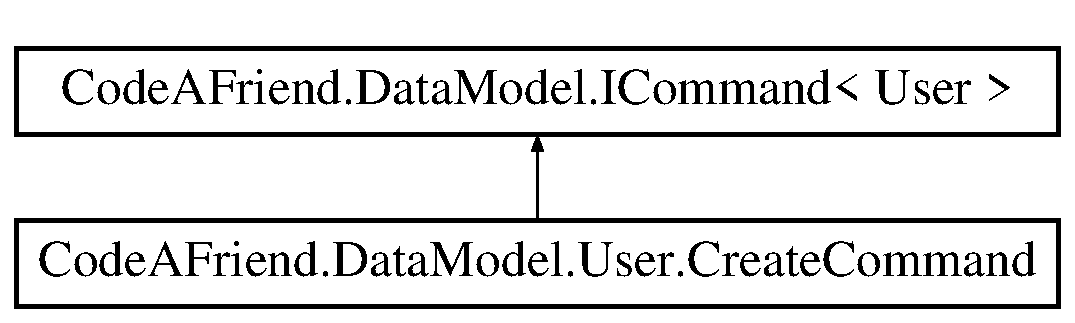
\includegraphics[height=2.000000cm]{class_code_a_friend_1_1_data_model_1_1_user_1_1_create_command}
\end{center}
\end{figure}
\subsection*{Public Member Functions}
\begin{DoxyCompactItemize}
\item 
\mbox{\hyperlink{class_code_a_friend_1_1_data_model_1_1_user_1_1_create_command_acf8bef896d5242b81824f379aa4144d1}{Create\+Command}} (string name)
\begin{DoxyCompactList}\small\item\em All properties constructor.\end{DoxyCompactList}\item 
async Task$<$ \mbox{\hyperlink{class_code_a_friend_1_1_data_model_1_1_user}{User}} $>$ \mbox{\hyperlink{class_code_a_friend_1_1_data_model_1_1_user_1_1_create_command_a83e6d841b7b008909b7b546d11cca7d6}{Execute\+Async}} (Db\+Context context)
\end{DoxyCompactItemize}
\subsection*{Properties}
\begin{DoxyCompactItemize}
\item 
string \mbox{\hyperlink{class_code_a_friend_1_1_data_model_1_1_user_1_1_create_command_a6f79ef49bd792a9d15ae1c74298bf11c}{Name}}\hspace{0.3cm}{\ttfamily  \mbox{[}get, set\mbox{]}}
\begin{DoxyCompactList}\small\item\em Name to be used to create the user.\end{DoxyCompactList}\end{DoxyCompactItemize}


\subsection{Detailed Description}
Properties someone can specify on user creation.



\subsection{Constructor \& Destructor Documentation}
\mbox{\Hypertarget{class_code_a_friend_1_1_data_model_1_1_user_1_1_create_command_acf8bef896d5242b81824f379aa4144d1}\label{class_code_a_friend_1_1_data_model_1_1_user_1_1_create_command_acf8bef896d5242b81824f379aa4144d1}} 
\index{Code\+A\+Friend\+::\+Data\+Model\+::\+User\+::\+Create\+Command@{Code\+A\+Friend\+::\+Data\+Model\+::\+User\+::\+Create\+Command}!Create\+Command@{Create\+Command}}
\index{Create\+Command@{Create\+Command}!Code\+A\+Friend\+::\+Data\+Model\+::\+User\+::\+Create\+Command@{Code\+A\+Friend\+::\+Data\+Model\+::\+User\+::\+Create\+Command}}
\subsubsection{\texorpdfstring{Create\+Command()}{CreateCommand()}}
{\footnotesize\ttfamily Code\+A\+Friend.\+Data\+Model.\+User.\+Create\+Command.\+Create\+Command (\begin{DoxyParamCaption}\item[{string}]{name }\end{DoxyParamCaption})}



All properties constructor.



\subsection{Member Function Documentation}
\mbox{\Hypertarget{class_code_a_friend_1_1_data_model_1_1_user_1_1_create_command_a83e6d841b7b008909b7b546d11cca7d6}\label{class_code_a_friend_1_1_data_model_1_1_user_1_1_create_command_a83e6d841b7b008909b7b546d11cca7d6}} 
\index{Code\+A\+Friend\+::\+Data\+Model\+::\+User\+::\+Create\+Command@{Code\+A\+Friend\+::\+Data\+Model\+::\+User\+::\+Create\+Command}!Execute\+Async@{Execute\+Async}}
\index{Execute\+Async@{Execute\+Async}!Code\+A\+Friend\+::\+Data\+Model\+::\+User\+::\+Create\+Command@{Code\+A\+Friend\+::\+Data\+Model\+::\+User\+::\+Create\+Command}}
\subsubsection{\texorpdfstring{Execute\+Async()}{ExecuteAsync()}}
{\footnotesize\ttfamily async Task$<$\mbox{\hyperlink{class_code_a_friend_1_1_data_model_1_1_user}{User}}$>$ Code\+A\+Friend.\+Data\+Model.\+User.\+Create\+Command.\+Execute\+Async (\begin{DoxyParamCaption}\item[{Db\+Context}]{context }\end{DoxyParamCaption})}







\subsection{Property Documentation}
\mbox{\Hypertarget{class_code_a_friend_1_1_data_model_1_1_user_1_1_create_command_a6f79ef49bd792a9d15ae1c74298bf11c}\label{class_code_a_friend_1_1_data_model_1_1_user_1_1_create_command_a6f79ef49bd792a9d15ae1c74298bf11c}} 
\index{Code\+A\+Friend\+::\+Data\+Model\+::\+User\+::\+Create\+Command@{Code\+A\+Friend\+::\+Data\+Model\+::\+User\+::\+Create\+Command}!Name@{Name}}
\index{Name@{Name}!Code\+A\+Friend\+::\+Data\+Model\+::\+User\+::\+Create\+Command@{Code\+A\+Friend\+::\+Data\+Model\+::\+User\+::\+Create\+Command}}
\subsubsection{\texorpdfstring{Name}{Name}}
{\footnotesize\ttfamily string Code\+A\+Friend.\+Data\+Model.\+User.\+Create\+Command.\+Name\hspace{0.3cm}{\ttfamily [get]}, {\ttfamily [set]}}



Name to be used to create the user.



The documentation for this class was generated from the following file\+:\begin{DoxyCompactItemize}
\item 
shared/\+Code\+A\+Friend.\+Data\+Model/\+User\+Logic/\mbox{\hyperlink{_user_8_commands_8cs}{User.\+Commands.\+cs}}\end{DoxyCompactItemize}

\hypertarget{class_code_a_friend_1_1_data_model_1_1_constants_1_1_default_execution_parameters}{}\section{Code\+A\+Friend.\+Data\+Model.\+Constants.\+Default\+Execution\+Parameters Class Reference}
\label{class_code_a_friend_1_1_data_model_1_1_constants_1_1_default_execution_parameters}\index{Code\+A\+Friend.\+Data\+Model.\+Constants.\+Default\+Execution\+Parameters@{Code\+A\+Friend.\+Data\+Model.\+Constants.\+Default\+Execution\+Parameters}}


Default execution parameters for any script running in an environment that does not specify the running parameters.  


Inheritance diagram for Code\+A\+Friend.\+Data\+Model.\+Constants.\+Default\+Execution\+Parameters\+:\begin{figure}[H]
\begin{center}
\leavevmode
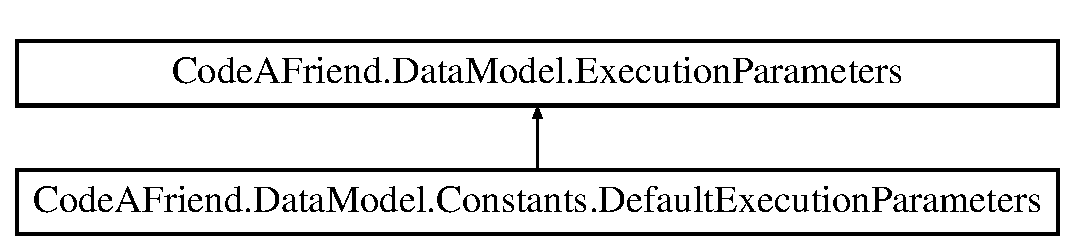
\includegraphics[height=2.000000cm]{class_code_a_friend_1_1_data_model_1_1_constants_1_1_default_execution_parameters}
\end{center}
\end{figure}
\subsection*{Public Member Functions}
\begin{DoxyCompactItemize}
\item 
\mbox{\hyperlink{class_code_a_friend_1_1_data_model_1_1_constants_1_1_default_execution_parameters_a5c8afe78939f6ba8052a2c0ccde9b4dc}{Default\+Execution\+Parameters}} ()
\item 
\mbox{\hyperlink{class_code_a_friend_1_1_data_model_1_1_constants_1_1_default_execution_parameters_a4e4c0663bfc96511b9d1d917c30804d3}{Default\+Execution\+Parameters}} (string input)
\end{DoxyCompactItemize}
\subsection*{Public Attributes}
\begin{DoxyCompactItemize}
\item 
const double \mbox{\hyperlink{class_code_a_friend_1_1_data_model_1_1_constants_1_1_default_execution_parameters_a0e3160be940c3cf873575fa86ddf9675}{M\+A\+X\+\_\+\+C\+P\+U\+\_\+\+T\+I\+ME}} = 5000
\begin{DoxyCompactList}\small\item\em Default maximum cpu time. \end{DoxyCompactList}\item 
const int \mbox{\hyperlink{class_code_a_friend_1_1_data_model_1_1_constants_1_1_default_execution_parameters_ae95dd594b14e585446672f9724b44d73}{M\+A\+X\+\_\+\+M\+E\+M\+O\+RY}} = 5000
\begin{DoxyCompactList}\small\item\em Default maximum memory usage. \end{DoxyCompactList}\end{DoxyCompactItemize}
\subsection*{Additional Inherited Members}


\subsection{Detailed Description}
Default execution parameters for any script running in an environment that does not specify the running parameters. 

Will be deprecated in the future in favor of a method that pulls these values from a config file.

\subsection{Constructor \& Destructor Documentation}
\mbox{\Hypertarget{class_code_a_friend_1_1_data_model_1_1_constants_1_1_default_execution_parameters_a5c8afe78939f6ba8052a2c0ccde9b4dc}\label{class_code_a_friend_1_1_data_model_1_1_constants_1_1_default_execution_parameters_a5c8afe78939f6ba8052a2c0ccde9b4dc}} 
\index{Code\+A\+Friend\+::\+Data\+Model\+::\+Constants\+::\+Default\+Execution\+Parameters@{Code\+A\+Friend\+::\+Data\+Model\+::\+Constants\+::\+Default\+Execution\+Parameters}!Default\+Execution\+Parameters@{Default\+Execution\+Parameters}}
\index{Default\+Execution\+Parameters@{Default\+Execution\+Parameters}!Code\+A\+Friend\+::\+Data\+Model\+::\+Constants\+::\+Default\+Execution\+Parameters@{Code\+A\+Friend\+::\+Data\+Model\+::\+Constants\+::\+Default\+Execution\+Parameters}}
\subsubsection{\texorpdfstring{Default\+Execution\+Parameters()}{DefaultExecutionParameters()}\hspace{0.1cm}{\footnotesize\ttfamily [1/2]}}
{\footnotesize\ttfamily Code\+A\+Friend.\+Data\+Model.\+Constants.\+Default\+Execution\+Parameters.\+Default\+Execution\+Parameters (\begin{DoxyParamCaption}{ }\end{DoxyParamCaption})}





\mbox{\Hypertarget{class_code_a_friend_1_1_data_model_1_1_constants_1_1_default_execution_parameters_a4e4c0663bfc96511b9d1d917c30804d3}\label{class_code_a_friend_1_1_data_model_1_1_constants_1_1_default_execution_parameters_a4e4c0663bfc96511b9d1d917c30804d3}} 
\index{Code\+A\+Friend\+::\+Data\+Model\+::\+Constants\+::\+Default\+Execution\+Parameters@{Code\+A\+Friend\+::\+Data\+Model\+::\+Constants\+::\+Default\+Execution\+Parameters}!Default\+Execution\+Parameters@{Default\+Execution\+Parameters}}
\index{Default\+Execution\+Parameters@{Default\+Execution\+Parameters}!Code\+A\+Friend\+::\+Data\+Model\+::\+Constants\+::\+Default\+Execution\+Parameters@{Code\+A\+Friend\+::\+Data\+Model\+::\+Constants\+::\+Default\+Execution\+Parameters}}
\subsubsection{\texorpdfstring{Default\+Execution\+Parameters()}{DefaultExecutionParameters()}\hspace{0.1cm}{\footnotesize\ttfamily [2/2]}}
{\footnotesize\ttfamily Code\+A\+Friend.\+Data\+Model.\+Constants.\+Default\+Execution\+Parameters.\+Default\+Execution\+Parameters (\begin{DoxyParamCaption}\item[{string}]{input }\end{DoxyParamCaption})}







\subsection{Member Data Documentation}
\mbox{\Hypertarget{class_code_a_friend_1_1_data_model_1_1_constants_1_1_default_execution_parameters_a0e3160be940c3cf873575fa86ddf9675}\label{class_code_a_friend_1_1_data_model_1_1_constants_1_1_default_execution_parameters_a0e3160be940c3cf873575fa86ddf9675}} 
\index{Code\+A\+Friend\+::\+Data\+Model\+::\+Constants\+::\+Default\+Execution\+Parameters@{Code\+A\+Friend\+::\+Data\+Model\+::\+Constants\+::\+Default\+Execution\+Parameters}!M\+A\+X\+\_\+\+C\+P\+U\+\_\+\+T\+I\+ME@{M\+A\+X\+\_\+\+C\+P\+U\+\_\+\+T\+I\+ME}}
\index{M\+A\+X\+\_\+\+C\+P\+U\+\_\+\+T\+I\+ME@{M\+A\+X\+\_\+\+C\+P\+U\+\_\+\+T\+I\+ME}!Code\+A\+Friend\+::\+Data\+Model\+::\+Constants\+::\+Default\+Execution\+Parameters@{Code\+A\+Friend\+::\+Data\+Model\+::\+Constants\+::\+Default\+Execution\+Parameters}}
\subsubsection{\texorpdfstring{M\+A\+X\+\_\+\+C\+P\+U\+\_\+\+T\+I\+ME}{MAX\_CPU\_TIME}}
{\footnotesize\ttfamily const double Code\+A\+Friend.\+Data\+Model.\+Constants.\+Default\+Execution\+Parameters.\+M\+A\+X\+\_\+\+C\+P\+U\+\_\+\+T\+I\+ME = 5000}



Default maximum cpu time. 

\mbox{\Hypertarget{class_code_a_friend_1_1_data_model_1_1_constants_1_1_default_execution_parameters_ae95dd594b14e585446672f9724b44d73}\label{class_code_a_friend_1_1_data_model_1_1_constants_1_1_default_execution_parameters_ae95dd594b14e585446672f9724b44d73}} 
\index{Code\+A\+Friend\+::\+Data\+Model\+::\+Constants\+::\+Default\+Execution\+Parameters@{Code\+A\+Friend\+::\+Data\+Model\+::\+Constants\+::\+Default\+Execution\+Parameters}!M\+A\+X\+\_\+\+M\+E\+M\+O\+RY@{M\+A\+X\+\_\+\+M\+E\+M\+O\+RY}}
\index{M\+A\+X\+\_\+\+M\+E\+M\+O\+RY@{M\+A\+X\+\_\+\+M\+E\+M\+O\+RY}!Code\+A\+Friend\+::\+Data\+Model\+::\+Constants\+::\+Default\+Execution\+Parameters@{Code\+A\+Friend\+::\+Data\+Model\+::\+Constants\+::\+Default\+Execution\+Parameters}}
\subsubsection{\texorpdfstring{M\+A\+X\+\_\+\+M\+E\+M\+O\+RY}{MAX\_MEMORY}}
{\footnotesize\ttfamily const int Code\+A\+Friend.\+Data\+Model.\+Constants.\+Default\+Execution\+Parameters.\+M\+A\+X\+\_\+\+M\+E\+M\+O\+RY = 5000}



Default maximum memory usage. 



The documentation for this class was generated from the following file\+:\begin{DoxyCompactItemize}
\item 
shared/\+Code\+A\+Friend.\+Data\+Model/\+Constants/\mbox{\hyperlink{_default_execution_parameters_8cs}{Default\+Execution\+Parameters.\+cs}}\end{DoxyCompactItemize}

\hypertarget{class_code_a_friend_1_1_data_model_1_1_user_1_1_delete_problem_command}{}\section{Code\+A\+Friend.\+Data\+Model.\+User.\+Delete\+Problem\+Command Class Reference}
\label{class_code_a_friend_1_1_data_model_1_1_user_1_1_delete_problem_command}\index{Code\+A\+Friend.\+Data\+Model.\+User.\+Delete\+Problem\+Command@{Code\+A\+Friend.\+Data\+Model.\+User.\+Delete\+Problem\+Command}}


 


Inheritance diagram for Code\+A\+Friend.\+Data\+Model.\+User.\+Delete\+Problem\+Command\+:\begin{figure}[H]
\begin{center}
\leavevmode
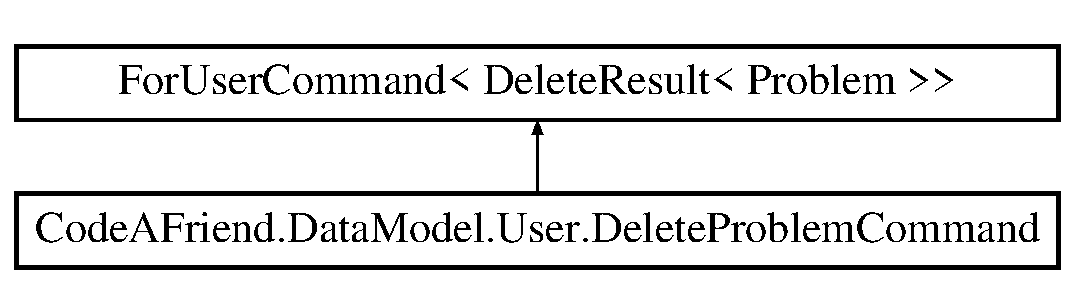
\includegraphics[height=2.000000cm]{class_code_a_friend_1_1_data_model_1_1_user_1_1_delete_problem_command}
\end{center}
\end{figure}
\subsection*{Public Member Functions}
\begin{DoxyCompactItemize}
\item 
\mbox{\hyperlink{class_code_a_friend_1_1_data_model_1_1_user_1_1_delete_problem_command_addb77111dd39c6d3baad2cf35dd308dd}{Delete\+Problem\+Command}} (string problem\+Name, string username)
\item 
override async Task$<$ \mbox{\hyperlink{class_code_a_friend_1_1_data_model_1_1_delete_result}{Delete\+Result}}$<$ \mbox{\hyperlink{class_code_a_friend_1_1_data_model_1_1_problem}{Problem}} $>$ $>$ \mbox{\hyperlink{class_code_a_friend_1_1_data_model_1_1_user_1_1_delete_problem_command_a5da058a13bbaad9487f34c3e16d347c9}{Execute\+Async}} (Db\+Context context)
\end{DoxyCompactItemize}
\subsection*{Properties}
\begin{DoxyCompactItemize}
\item 
string \mbox{\hyperlink{class_code_a_friend_1_1_data_model_1_1_user_1_1_delete_problem_command_a220adc216f07aeed2119eb4dc946de21}{Problem\+Name}}\hspace{0.3cm}{\ttfamily  \mbox{[}get, set\mbox{]}}
\begin{DoxyCompactList}\small\item\em Id of the \mbox{\hyperlink{class_code_a_friend_1_1_data_model_1_1_problem}{Problem}} to operate on.\end{DoxyCompactList}\end{DoxyCompactItemize}


\subsection{Detailed Description}


\subsection{Constructor \& Destructor Documentation}
\mbox{\Hypertarget{class_code_a_friend_1_1_data_model_1_1_user_1_1_delete_problem_command_addb77111dd39c6d3baad2cf35dd308dd}\label{class_code_a_friend_1_1_data_model_1_1_user_1_1_delete_problem_command_addb77111dd39c6d3baad2cf35dd308dd}} 
\index{Code\+A\+Friend\+::\+Data\+Model\+::\+User\+::\+Delete\+Problem\+Command@{Code\+A\+Friend\+::\+Data\+Model\+::\+User\+::\+Delete\+Problem\+Command}!Delete\+Problem\+Command@{Delete\+Problem\+Command}}
\index{Delete\+Problem\+Command@{Delete\+Problem\+Command}!Code\+A\+Friend\+::\+Data\+Model\+::\+User\+::\+Delete\+Problem\+Command@{Code\+A\+Friend\+::\+Data\+Model\+::\+User\+::\+Delete\+Problem\+Command}}
\subsubsection{\texorpdfstring{Delete\+Problem\+Command()}{DeleteProblemCommand()}}
{\footnotesize\ttfamily Code\+A\+Friend.\+Data\+Model.\+User.\+Delete\+Problem\+Command.\+Delete\+Problem\+Command (\begin{DoxyParamCaption}\item[{string}]{problem\+Name,  }\item[{string}]{username }\end{DoxyParamCaption})}







\subsection{Member Function Documentation}
\mbox{\Hypertarget{class_code_a_friend_1_1_data_model_1_1_user_1_1_delete_problem_command_a5da058a13bbaad9487f34c3e16d347c9}\label{class_code_a_friend_1_1_data_model_1_1_user_1_1_delete_problem_command_a5da058a13bbaad9487f34c3e16d347c9}} 
\index{Code\+A\+Friend\+::\+Data\+Model\+::\+User\+::\+Delete\+Problem\+Command@{Code\+A\+Friend\+::\+Data\+Model\+::\+User\+::\+Delete\+Problem\+Command}!Execute\+Async@{Execute\+Async}}
\index{Execute\+Async@{Execute\+Async}!Code\+A\+Friend\+::\+Data\+Model\+::\+User\+::\+Delete\+Problem\+Command@{Code\+A\+Friend\+::\+Data\+Model\+::\+User\+::\+Delete\+Problem\+Command}}
\subsubsection{\texorpdfstring{Execute\+Async()}{ExecuteAsync()}}
{\footnotesize\ttfamily override async Task$<$\mbox{\hyperlink{class_code_a_friend_1_1_data_model_1_1_delete_result}{Delete\+Result}}$<$\mbox{\hyperlink{class_code_a_friend_1_1_data_model_1_1_problem}{Problem}}$>$ $>$ Code\+A\+Friend.\+Data\+Model.\+User.\+Delete\+Problem\+Command.\+Execute\+Async (\begin{DoxyParamCaption}\item[{Db\+Context}]{context }\end{DoxyParamCaption})}







\subsection{Property Documentation}
\mbox{\Hypertarget{class_code_a_friend_1_1_data_model_1_1_user_1_1_delete_problem_command_a220adc216f07aeed2119eb4dc946de21}\label{class_code_a_friend_1_1_data_model_1_1_user_1_1_delete_problem_command_a220adc216f07aeed2119eb4dc946de21}} 
\index{Code\+A\+Friend\+::\+Data\+Model\+::\+User\+::\+Delete\+Problem\+Command@{Code\+A\+Friend\+::\+Data\+Model\+::\+User\+::\+Delete\+Problem\+Command}!Problem\+Name@{Problem\+Name}}
\index{Problem\+Name@{Problem\+Name}!Code\+A\+Friend\+::\+Data\+Model\+::\+User\+::\+Delete\+Problem\+Command@{Code\+A\+Friend\+::\+Data\+Model\+::\+User\+::\+Delete\+Problem\+Command}}
\subsubsection{\texorpdfstring{Problem\+Name}{ProblemName}}
{\footnotesize\ttfamily string Code\+A\+Friend.\+Data\+Model.\+User.\+Delete\+Problem\+Command.\+Problem\+Name\hspace{0.3cm}{\ttfamily [get]}, {\ttfamily [set]}}



Id of the \mbox{\hyperlink{class_code_a_friend_1_1_data_model_1_1_problem}{Problem}} to operate on.



The documentation for this class was generated from the following file\+:\begin{DoxyCompactItemize}
\item 
shared/\+Code\+A\+Friend.\+Data\+Model/\+User\+Logic/\mbox{\hyperlink{_user_8_problem_commands_8cs}{User.\+Problem\+Commands.\+cs}}\end{DoxyCompactItemize}

\hypertarget{class_code_a_friend_1_1_data_model_1_1_delete_result}{}\section{Code\+A\+Friend.\+Data\+Model.\+Delete\+Result$<$ T\+Value $>$ Class Template Reference}
\label{class_code_a_friend_1_1_data_model_1_1_delete_result}\index{Code\+A\+Friend.\+Data\+Model.\+Delete\+Result$<$ T\+Value $>$@{Code\+A\+Friend.\+Data\+Model.\+Delete\+Result$<$ T\+Value $>$}}


Represents an entity that has been deleted.  




\subsection{Detailed Description}
Represents an entity that has been deleted. 


\begin{DoxyTemplParams}{Template Parameters}
{\em T\+Value} & Type of the deleted entity\\
\hline
\end{DoxyTemplParams}


The documentation for this class was generated from the following file\+:\begin{DoxyCompactItemize}
\item 
shared/\+Code\+A\+Friend.\+Data\+Model/\mbox{\hyperlink{_delete_result_8cs}{Delete\+Result.\+cs}}\end{DoxyCompactItemize}

\hypertarget{class_code_a_friend_1_1_data_model_1_1_user_1_1_delete_script_command}{}\section{Code\+A\+Friend.\+Data\+Model.\+User.\+Delete\+Script\+Command Class Reference}
\label{class_code_a_friend_1_1_data_model_1_1_user_1_1_delete_script_command}\index{Code\+A\+Friend.\+Data\+Model.\+User.\+Delete\+Script\+Command@{Code\+A\+Friend.\+Data\+Model.\+User.\+Delete\+Script\+Command}}


 


Inheritance diagram for Code\+A\+Friend.\+Data\+Model.\+User.\+Delete\+Script\+Command\+:\begin{figure}[H]
\begin{center}
\leavevmode
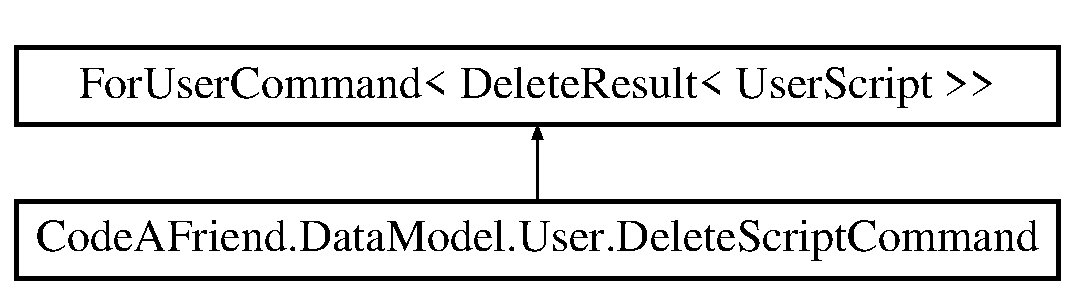
\includegraphics[height=2.000000cm]{class_code_a_friend_1_1_data_model_1_1_user_1_1_delete_script_command}
\end{center}
\end{figure}
\subsection*{Public Member Functions}
\begin{DoxyCompactItemize}
\item 
\mbox{\hyperlink{class_code_a_friend_1_1_data_model_1_1_user_1_1_delete_script_command_ac02256e361e53c6ae44efff19ee2f74d}{Delete\+Script\+Command}} (Guid script\+Id, string username)
\item 
override async Task$<$ \mbox{\hyperlink{class_code_a_friend_1_1_data_model_1_1_delete_result}{Delete\+Result}}$<$ \mbox{\hyperlink{class_code_a_friend_1_1_data_model_1_1_user_script}{User\+Script}} $>$ $>$ \mbox{\hyperlink{class_code_a_friend_1_1_data_model_1_1_user_1_1_delete_script_command_aef17563b2ed3bd6fc460fc9c7bbb2024}{Execute\+Async}} (Db\+Context context)
\end{DoxyCompactItemize}
\subsection*{Properties}
\begin{DoxyCompactItemize}
\item 
Guid \mbox{\hyperlink{class_code_a_friend_1_1_data_model_1_1_user_1_1_delete_script_command_a1f857c62d2d1e84239b98a892ebe8da7}{Script\+Id}}\hspace{0.3cm}{\ttfamily  \mbox{[}get, set\mbox{]}}
\begin{DoxyCompactList}\small\item\em Id of the \mbox{\hyperlink{class_code_a_friend_1_1_data_model_1_1_script}{Script}} to operate on.\end{DoxyCompactList}\end{DoxyCompactItemize}


\subsection{Detailed Description}


\subsection{Constructor \& Destructor Documentation}
\mbox{\Hypertarget{class_code_a_friend_1_1_data_model_1_1_user_1_1_delete_script_command_ac02256e361e53c6ae44efff19ee2f74d}\label{class_code_a_friend_1_1_data_model_1_1_user_1_1_delete_script_command_ac02256e361e53c6ae44efff19ee2f74d}} 
\index{Code\+A\+Friend\+::\+Data\+Model\+::\+User\+::\+Delete\+Script\+Command@{Code\+A\+Friend\+::\+Data\+Model\+::\+User\+::\+Delete\+Script\+Command}!Delete\+Script\+Command@{Delete\+Script\+Command}}
\index{Delete\+Script\+Command@{Delete\+Script\+Command}!Code\+A\+Friend\+::\+Data\+Model\+::\+User\+::\+Delete\+Script\+Command@{Code\+A\+Friend\+::\+Data\+Model\+::\+User\+::\+Delete\+Script\+Command}}
\subsubsection{\texorpdfstring{Delete\+Script\+Command()}{DeleteScriptCommand()}}
{\footnotesize\ttfamily Code\+A\+Friend.\+Data\+Model.\+User.\+Delete\+Script\+Command.\+Delete\+Script\+Command (\begin{DoxyParamCaption}\item[{Guid}]{script\+Id,  }\item[{string}]{username }\end{DoxyParamCaption})}







\subsection{Member Function Documentation}
\mbox{\Hypertarget{class_code_a_friend_1_1_data_model_1_1_user_1_1_delete_script_command_aef17563b2ed3bd6fc460fc9c7bbb2024}\label{class_code_a_friend_1_1_data_model_1_1_user_1_1_delete_script_command_aef17563b2ed3bd6fc460fc9c7bbb2024}} 
\index{Code\+A\+Friend\+::\+Data\+Model\+::\+User\+::\+Delete\+Script\+Command@{Code\+A\+Friend\+::\+Data\+Model\+::\+User\+::\+Delete\+Script\+Command}!Execute\+Async@{Execute\+Async}}
\index{Execute\+Async@{Execute\+Async}!Code\+A\+Friend\+::\+Data\+Model\+::\+User\+::\+Delete\+Script\+Command@{Code\+A\+Friend\+::\+Data\+Model\+::\+User\+::\+Delete\+Script\+Command}}
\subsubsection{\texorpdfstring{Execute\+Async()}{ExecuteAsync()}}
{\footnotesize\ttfamily override async Task$<$\mbox{\hyperlink{class_code_a_friend_1_1_data_model_1_1_delete_result}{Delete\+Result}}$<$\mbox{\hyperlink{class_code_a_friend_1_1_data_model_1_1_user_script}{User\+Script}}$>$ $>$ Code\+A\+Friend.\+Data\+Model.\+User.\+Delete\+Script\+Command.\+Execute\+Async (\begin{DoxyParamCaption}\item[{Db\+Context}]{context }\end{DoxyParamCaption})}







\subsection{Property Documentation}
\mbox{\Hypertarget{class_code_a_friend_1_1_data_model_1_1_user_1_1_delete_script_command_a1f857c62d2d1e84239b98a892ebe8da7}\label{class_code_a_friend_1_1_data_model_1_1_user_1_1_delete_script_command_a1f857c62d2d1e84239b98a892ebe8da7}} 
\index{Code\+A\+Friend\+::\+Data\+Model\+::\+User\+::\+Delete\+Script\+Command@{Code\+A\+Friend\+::\+Data\+Model\+::\+User\+::\+Delete\+Script\+Command}!Script\+Id@{Script\+Id}}
\index{Script\+Id@{Script\+Id}!Code\+A\+Friend\+::\+Data\+Model\+::\+User\+::\+Delete\+Script\+Command@{Code\+A\+Friend\+::\+Data\+Model\+::\+User\+::\+Delete\+Script\+Command}}
\subsubsection{\texorpdfstring{Script\+Id}{ScriptId}}
{\footnotesize\ttfamily Guid Code\+A\+Friend.\+Data\+Model.\+User.\+Delete\+Script\+Command.\+Script\+Id\hspace{0.3cm}{\ttfamily [get]}, {\ttfamily [set]}}



Id of the \mbox{\hyperlink{class_code_a_friend_1_1_data_model_1_1_script}{Script}} to operate on.



The documentation for this class was generated from the following file\+:\begin{DoxyCompactItemize}
\item 
shared/\+Code\+A\+Friend.\+Data\+Model/\+User\+Logic/\mbox{\hyperlink{_user_8_script_commands_8cs}{User.\+Script\+Commands.\+cs}}\end{DoxyCompactItemize}

\hypertarget{class_code_a_friend_1_1_api_service_1_1_models_1_1_error_view_model}{}\section{Code\+A\+Friend.\+Api\+Service.\+Models.\+Error\+View\+Model Class Reference}
\label{class_code_a_friend_1_1_api_service_1_1_models_1_1_error_view_model}\index{Code\+A\+Friend.\+Api\+Service.\+Models.\+Error\+View\+Model@{Code\+A\+Friend.\+Api\+Service.\+Models.\+Error\+View\+Model}}
\subsection*{Public Attributes}
\begin{DoxyCompactItemize}
\item 
bool \mbox{\hyperlink{class_code_a_friend_1_1_api_service_1_1_models_1_1_error_view_model_a8bc3d8ee7b7604516c1ac54b7080c761}{Show\+Request\+Id}} =$>$ !string.\+Is\+Null\+Or\+Empty(\mbox{\hyperlink{class_code_a_friend_1_1_api_service_1_1_models_1_1_error_view_model_aa19824bbfb14fe33283a6c282b653388}{Request\+Id}})
\end{DoxyCompactItemize}
\subsection*{Properties}
\begin{DoxyCompactItemize}
\item 
string \mbox{\hyperlink{class_code_a_friend_1_1_api_service_1_1_models_1_1_error_view_model_aa19824bbfb14fe33283a6c282b653388}{Request\+Id}}\hspace{0.3cm}{\ttfamily  \mbox{[}get, set\mbox{]}}
\end{DoxyCompactItemize}


\subsection{Member Data Documentation}
\mbox{\Hypertarget{class_code_a_friend_1_1_api_service_1_1_models_1_1_error_view_model_a8bc3d8ee7b7604516c1ac54b7080c761}\label{class_code_a_friend_1_1_api_service_1_1_models_1_1_error_view_model_a8bc3d8ee7b7604516c1ac54b7080c761}} 
\index{Code\+A\+Friend\+::\+Api\+Service\+::\+Models\+::\+Error\+View\+Model@{Code\+A\+Friend\+::\+Api\+Service\+::\+Models\+::\+Error\+View\+Model}!Show\+Request\+Id@{Show\+Request\+Id}}
\index{Show\+Request\+Id@{Show\+Request\+Id}!Code\+A\+Friend\+::\+Api\+Service\+::\+Models\+::\+Error\+View\+Model@{Code\+A\+Friend\+::\+Api\+Service\+::\+Models\+::\+Error\+View\+Model}}
\subsubsection{\texorpdfstring{Show\+Request\+Id}{ShowRequestId}}
{\footnotesize\ttfamily bool Code\+A\+Friend.\+Api\+Service.\+Models.\+Error\+View\+Model.\+Show\+Request\+Id =$>$ !string.\+Is\+Null\+Or\+Empty(\mbox{\hyperlink{class_code_a_friend_1_1_api_service_1_1_models_1_1_error_view_model_aa19824bbfb14fe33283a6c282b653388}{Request\+Id}})}



\subsection{Property Documentation}
\mbox{\Hypertarget{class_code_a_friend_1_1_api_service_1_1_models_1_1_error_view_model_aa19824bbfb14fe33283a6c282b653388}\label{class_code_a_friend_1_1_api_service_1_1_models_1_1_error_view_model_aa19824bbfb14fe33283a6c282b653388}} 
\index{Code\+A\+Friend\+::\+Api\+Service\+::\+Models\+::\+Error\+View\+Model@{Code\+A\+Friend\+::\+Api\+Service\+::\+Models\+::\+Error\+View\+Model}!Request\+Id@{Request\+Id}}
\index{Request\+Id@{Request\+Id}!Code\+A\+Friend\+::\+Api\+Service\+::\+Models\+::\+Error\+View\+Model@{Code\+A\+Friend\+::\+Api\+Service\+::\+Models\+::\+Error\+View\+Model}}
\subsubsection{\texorpdfstring{Request\+Id}{RequestId}}
{\footnotesize\ttfamily string Code\+A\+Friend.\+Api\+Service.\+Models.\+Error\+View\+Model.\+Request\+Id\hspace{0.3cm}{\ttfamily [get]}, {\ttfamily [set]}}



The documentation for this class was generated from the following file\+:\begin{DoxyCompactItemize}
\item 
apps/\+Code\+A\+Friend.\+Api\+Service/\+Models/\mbox{\hyperlink{_error_view_model_8cs}{Error\+View\+Model.\+cs}}\end{DoxyCompactItemize}

\hypertarget{class_code_a_friend_1_1_data_model_1_1_execution_parameters}{}\section{Code\+A\+Friend.\+Data\+Model.\+Execution\+Parameters Class Reference}
\label{class_code_a_friend_1_1_data_model_1_1_execution_parameters}\index{Code\+A\+Friend.\+Data\+Model.\+Execution\+Parameters@{Code\+A\+Friend.\+Data\+Model.\+Execution\+Parameters}}


Parameters to use when executing code.  


Inheritance diagram for Code\+A\+Friend.\+Data\+Model.\+Execution\+Parameters\+:\begin{figure}[H]
\begin{center}
\leavevmode
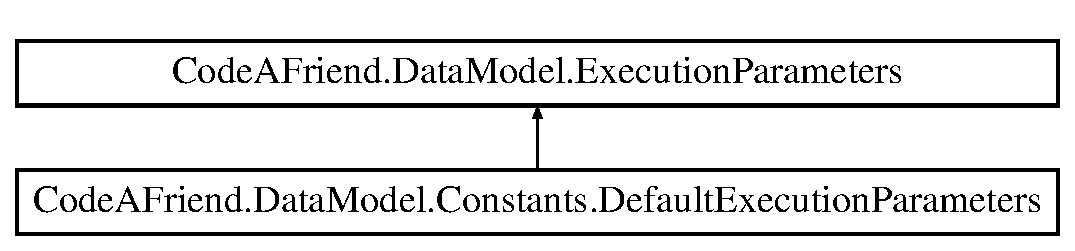
\includegraphics[height=2.000000cm]{class_code_a_friend_1_1_data_model_1_1_execution_parameters}
\end{center}
\end{figure}
\subsection*{Public Member Functions}
\begin{DoxyCompactItemize}
\item 
\mbox{\hyperlink{class_code_a_friend_1_1_data_model_1_1_execution_parameters_ad64d2dbe0d229005a3ca8ec620525cdf}{Execution\+Parameters}} (double max\+Cpu\+Time, long max\+Memory, string input)
\begin{DoxyCompactList}\small\item\em All Properties constructor. \end{DoxyCompactList}\end{DoxyCompactItemize}
\subsection*{Properties}
\begin{DoxyCompactItemize}
\item 
double \mbox{\hyperlink{class_code_a_friend_1_1_data_model_1_1_execution_parameters_a3a919b6815a5945ecc04a4d388a2962c}{Max\+Cpu\+Time}}\hspace{0.3cm}{\ttfamily  \mbox{[}get, set\mbox{]}}
\begin{DoxyCompactList}\small\item\em Maximum amount of time in ms that the code should be allowed to execute. \end{DoxyCompactList}\item 
long \mbox{\hyperlink{class_code_a_friend_1_1_data_model_1_1_execution_parameters_a8fa68ab9aabe8993245a26541d2256c6}{Max\+Memory}}\hspace{0.3cm}{\ttfamily  \mbox{[}get, set\mbox{]}}
\begin{DoxyCompactList}\small\item\em Maximum amount of memory (in kB) that the code should be allowed to allocate during execution. \end{DoxyCompactList}\item 
string \mbox{\hyperlink{class_code_a_friend_1_1_data_model_1_1_execution_parameters_a7d693e2b7e6696606e29a083792c4cc6}{Input}}\hspace{0.3cm}{\ttfamily  \mbox{[}get, set\mbox{]}}
\begin{DoxyCompactList}\small\item\em Input to provide to stdin during program execution. \end{DoxyCompactList}\end{DoxyCompactItemize}


\subsection{Detailed Description}
Parameters to use when executing code. 



\subsection{Constructor \& Destructor Documentation}
\mbox{\Hypertarget{class_code_a_friend_1_1_data_model_1_1_execution_parameters_ad64d2dbe0d229005a3ca8ec620525cdf}\label{class_code_a_friend_1_1_data_model_1_1_execution_parameters_ad64d2dbe0d229005a3ca8ec620525cdf}} 
\index{Code\+A\+Friend\+::\+Data\+Model\+::\+Execution\+Parameters@{Code\+A\+Friend\+::\+Data\+Model\+::\+Execution\+Parameters}!Execution\+Parameters@{Execution\+Parameters}}
\index{Execution\+Parameters@{Execution\+Parameters}!Code\+A\+Friend\+::\+Data\+Model\+::\+Execution\+Parameters@{Code\+A\+Friend\+::\+Data\+Model\+::\+Execution\+Parameters}}
\subsubsection{\texorpdfstring{Execution\+Parameters()}{ExecutionParameters()}}
{\footnotesize\ttfamily Code\+A\+Friend.\+Data\+Model.\+Execution\+Parameters.\+Execution\+Parameters (\begin{DoxyParamCaption}\item[{double}]{max\+Cpu\+Time,  }\item[{long}]{max\+Memory,  }\item[{string}]{input }\end{DoxyParamCaption})}



All Properties constructor. 



\subsection{Property Documentation}
\mbox{\Hypertarget{class_code_a_friend_1_1_data_model_1_1_execution_parameters_a7d693e2b7e6696606e29a083792c4cc6}\label{class_code_a_friend_1_1_data_model_1_1_execution_parameters_a7d693e2b7e6696606e29a083792c4cc6}} 
\index{Code\+A\+Friend\+::\+Data\+Model\+::\+Execution\+Parameters@{Code\+A\+Friend\+::\+Data\+Model\+::\+Execution\+Parameters}!Input@{Input}}
\index{Input@{Input}!Code\+A\+Friend\+::\+Data\+Model\+::\+Execution\+Parameters@{Code\+A\+Friend\+::\+Data\+Model\+::\+Execution\+Parameters}}
\subsubsection{\texorpdfstring{Input}{Input}}
{\footnotesize\ttfamily string Code\+A\+Friend.\+Data\+Model.\+Execution\+Parameters.\+Input\hspace{0.3cm}{\ttfamily [get]}, {\ttfamily [set]}}



Input to provide to stdin during program execution. 

\mbox{\Hypertarget{class_code_a_friend_1_1_data_model_1_1_execution_parameters_a3a919b6815a5945ecc04a4d388a2962c}\label{class_code_a_friend_1_1_data_model_1_1_execution_parameters_a3a919b6815a5945ecc04a4d388a2962c}} 
\index{Code\+A\+Friend\+::\+Data\+Model\+::\+Execution\+Parameters@{Code\+A\+Friend\+::\+Data\+Model\+::\+Execution\+Parameters}!Max\+Cpu\+Time@{Max\+Cpu\+Time}}
\index{Max\+Cpu\+Time@{Max\+Cpu\+Time}!Code\+A\+Friend\+::\+Data\+Model\+::\+Execution\+Parameters@{Code\+A\+Friend\+::\+Data\+Model\+::\+Execution\+Parameters}}
\subsubsection{\texorpdfstring{Max\+Cpu\+Time}{MaxCpuTime}}
{\footnotesize\ttfamily double Code\+A\+Friend.\+Data\+Model.\+Execution\+Parameters.\+Max\+Cpu\+Time\hspace{0.3cm}{\ttfamily [get]}, {\ttfamily [set]}}



Maximum amount of time in ms that the code should be allowed to execute. 

\mbox{\Hypertarget{class_code_a_friend_1_1_data_model_1_1_execution_parameters_a8fa68ab9aabe8993245a26541d2256c6}\label{class_code_a_friend_1_1_data_model_1_1_execution_parameters_a8fa68ab9aabe8993245a26541d2256c6}} 
\index{Code\+A\+Friend\+::\+Data\+Model\+::\+Execution\+Parameters@{Code\+A\+Friend\+::\+Data\+Model\+::\+Execution\+Parameters}!Max\+Memory@{Max\+Memory}}
\index{Max\+Memory@{Max\+Memory}!Code\+A\+Friend\+::\+Data\+Model\+::\+Execution\+Parameters@{Code\+A\+Friend\+::\+Data\+Model\+::\+Execution\+Parameters}}
\subsubsection{\texorpdfstring{Max\+Memory}{MaxMemory}}
{\footnotesize\ttfamily long Code\+A\+Friend.\+Data\+Model.\+Execution\+Parameters.\+Max\+Memory\hspace{0.3cm}{\ttfamily [get]}, {\ttfamily [set]}}



Maximum amount of memory (in kB) that the code should be allowed to allocate during execution. 



The documentation for this class was generated from the following file\+:\begin{DoxyCompactItemize}
\item 
shared/\+Code\+A\+Friend.\+Data\+Model/\+Script\+Logic/\mbox{\hyperlink{_execution_parameters_8cs}{Execution\+Parameters.\+cs}}\end{DoxyCompactItemize}

\hypertarget{class_code_a_friend_1_1_data_model_1_1_user_1_1_for_user_command}{}\section{Code\+A\+Friend.\+Data\+Model.\+User.\+For\+User\+Command$<$ T\+Result $>$ Class Template Reference}
\label{class_code_a_friend_1_1_data_model_1_1_user_1_1_for_user_command}\index{Code\+A\+Friend.\+Data\+Model.\+User.\+For\+User\+Command$<$ T\+Result $>$@{Code\+A\+Friend.\+Data\+Model.\+User.\+For\+User\+Command$<$ T\+Result $>$}}


Command being performed on behalf of a specific user. 


Inheritance diagram for Code\+A\+Friend.\+Data\+Model.\+User.\+For\+User\+Command$<$ T\+Result $>$\+:\begin{figure}[H]
\begin{center}
\leavevmode
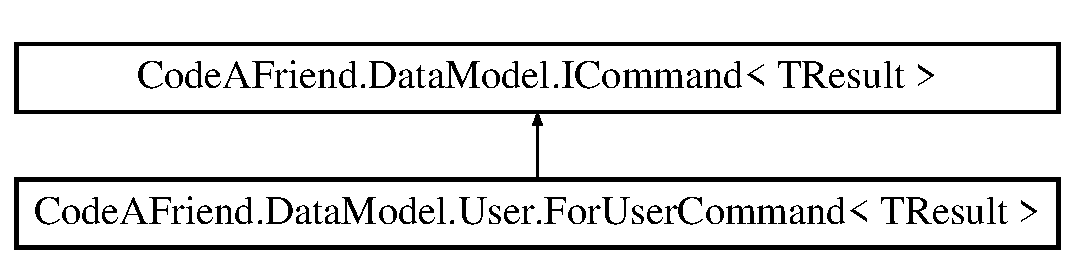
\includegraphics[height=2.000000cm]{class_code_a_friend_1_1_data_model_1_1_user_1_1_for_user_command}
\end{center}
\end{figure}
\subsection*{Public Member Functions}
\begin{DoxyCompactItemize}
\item 
abstract Task$<$ T\+Result $>$ \mbox{\hyperlink{class_code_a_friend_1_1_data_model_1_1_user_1_1_for_user_command_aa9abf9da11dd2a573d8ed93bcf53f6df}{Execute\+Async}} (Db\+Context context)
\end{DoxyCompactItemize}
\subsection*{Protected Member Functions}
\begin{DoxyCompactItemize}
\item 
\mbox{\hyperlink{class_code_a_friend_1_1_data_model_1_1_user_1_1_for_user_command_ae8e4225f2733cef42a531d4a30ba1b3e}{For\+User\+Command}} (string username)
\begin{DoxyCompactList}\small\item\em All properties constructor.\end{DoxyCompactList}\end{DoxyCompactItemize}
\subsection*{Properties}
\begin{DoxyCompactItemize}
\item 
string \mbox{\hyperlink{class_code_a_friend_1_1_data_model_1_1_user_1_1_for_user_command_a2c7fef551c3661f0bc712733d1b1380d}{Username}}\hspace{0.3cm}{\ttfamily  \mbox{[}get, set\mbox{]}}
\begin{DoxyCompactList}\small\item\em Name of the user this operation is for.\end{DoxyCompactList}\end{DoxyCompactItemize}


\subsection{Detailed Description}
Command being performed on behalf of a specific user.



\subsection{Constructor \& Destructor Documentation}
\mbox{\Hypertarget{class_code_a_friend_1_1_data_model_1_1_user_1_1_for_user_command_ae8e4225f2733cef42a531d4a30ba1b3e}\label{class_code_a_friend_1_1_data_model_1_1_user_1_1_for_user_command_ae8e4225f2733cef42a531d4a30ba1b3e}} 
\index{Code\+A\+Friend\+::\+Data\+Model\+::\+User\+::\+For\+User\+Command@{Code\+A\+Friend\+::\+Data\+Model\+::\+User\+::\+For\+User\+Command}!For\+User\+Command@{For\+User\+Command}}
\index{For\+User\+Command@{For\+User\+Command}!Code\+A\+Friend\+::\+Data\+Model\+::\+User\+::\+For\+User\+Command@{Code\+A\+Friend\+::\+Data\+Model\+::\+User\+::\+For\+User\+Command}}
\subsubsection{\texorpdfstring{For\+User\+Command()}{ForUserCommand()}}
{\footnotesize\ttfamily \mbox{\hyperlink{class_code_a_friend_1_1_data_model_1_1_user_1_1_for_user_command}{Code\+A\+Friend.\+Data\+Model.\+User.\+For\+User\+Command}}$<$ T\+Result $>$.\mbox{\hyperlink{class_code_a_friend_1_1_data_model_1_1_user_1_1_for_user_command}{For\+User\+Command}} (\begin{DoxyParamCaption}\item[{string}]{username }\end{DoxyParamCaption})\hspace{0.3cm}{\ttfamily [protected]}}



All properties constructor.



\subsection{Member Function Documentation}
\mbox{\Hypertarget{class_code_a_friend_1_1_data_model_1_1_user_1_1_for_user_command_aa9abf9da11dd2a573d8ed93bcf53f6df}\label{class_code_a_friend_1_1_data_model_1_1_user_1_1_for_user_command_aa9abf9da11dd2a573d8ed93bcf53f6df}} 
\index{Code\+A\+Friend\+::\+Data\+Model\+::\+User\+::\+For\+User\+Command@{Code\+A\+Friend\+::\+Data\+Model\+::\+User\+::\+For\+User\+Command}!Execute\+Async@{Execute\+Async}}
\index{Execute\+Async@{Execute\+Async}!Code\+A\+Friend\+::\+Data\+Model\+::\+User\+::\+For\+User\+Command@{Code\+A\+Friend\+::\+Data\+Model\+::\+User\+::\+For\+User\+Command}}
\subsubsection{\texorpdfstring{Execute\+Async()}{ExecuteAsync()}}
{\footnotesize\ttfamily abstract Task$<$T\+Result$>$ \mbox{\hyperlink{class_code_a_friend_1_1_data_model_1_1_user_1_1_for_user_command}{Code\+A\+Friend.\+Data\+Model.\+User.\+For\+User\+Command}}$<$ T\+Result $>$.Execute\+Async (\begin{DoxyParamCaption}\item[{Db\+Context}]{context }\end{DoxyParamCaption})\hspace{0.3cm}{\ttfamily [pure virtual]}}







Implemented in \mbox{\hyperlink{class_code_a_friend_1_1_data_model_1_1_user_1_1_update_script_command_a54e74e6d68bfc5e01cbcc96fd6dfbd2d}{Code\+A\+Friend.\+Data\+Model.\+User.\+Update\+Script\+Command}}, \mbox{\hyperlink{class_code_a_friend_1_1_data_model_1_1_user_1_1_update_problem_command_ab6deb9c81098f15347a52cff94661c4b}{Code\+A\+Friend.\+Data\+Model.\+User.\+Update\+Problem\+Command}}, \mbox{\hyperlink{class_code_a_friend_1_1_data_model_1_1_user_1_1_add_script_command_a7105f586c7502c18a3ac2cfd567c90f0}{Code\+A\+Friend.\+Data\+Model.\+User.\+Add\+Script\+Command}}, and \mbox{\hyperlink{class_code_a_friend_1_1_data_model_1_1_user_1_1_add_problem_command_a43eff118c9d451d384008fe68559d50d}{Code\+A\+Friend.\+Data\+Model.\+User.\+Add\+Problem\+Command}}.



\subsection{Property Documentation}
\mbox{\Hypertarget{class_code_a_friend_1_1_data_model_1_1_user_1_1_for_user_command_a2c7fef551c3661f0bc712733d1b1380d}\label{class_code_a_friend_1_1_data_model_1_1_user_1_1_for_user_command_a2c7fef551c3661f0bc712733d1b1380d}} 
\index{Code\+A\+Friend\+::\+Data\+Model\+::\+User\+::\+For\+User\+Command@{Code\+A\+Friend\+::\+Data\+Model\+::\+User\+::\+For\+User\+Command}!Username@{Username}}
\index{Username@{Username}!Code\+A\+Friend\+::\+Data\+Model\+::\+User\+::\+For\+User\+Command@{Code\+A\+Friend\+::\+Data\+Model\+::\+User\+::\+For\+User\+Command}}
\subsubsection{\texorpdfstring{Username}{Username}}
{\footnotesize\ttfamily string \mbox{\hyperlink{class_code_a_friend_1_1_data_model_1_1_user_1_1_for_user_command}{Code\+A\+Friend.\+Data\+Model.\+User.\+For\+User\+Command}}$<$ T\+Result $>$.Username\hspace{0.3cm}{\ttfamily [get]}, {\ttfamily [set]}}



Name of the user this operation is for.



The documentation for this class was generated from the following file\+:\begin{DoxyCompactItemize}
\item 
shared/\+Code\+A\+Friend.\+Data\+Model/\+User\+Logic/\mbox{\hyperlink{_user_8_commands_8cs}{User.\+Commands.\+cs}}\end{DoxyCompactItemize}

\hypertarget{interface_code_a_friend_1_1_facade_1_1_i_code_a_friend_facade}{}\section{Code\+A\+Friend.\+Facade.\+I\+Code\+A\+Friend\+Facade Interface Reference}
\label{interface_code_a_friend_1_1_facade_1_1_i_code_a_friend_facade}\index{Code\+A\+Friend.\+Facade.\+I\+Code\+A\+Friend\+Facade@{Code\+A\+Friend.\+Facade.\+I\+Code\+A\+Friend\+Facade}}


Exposes stored user objects for the \mbox{\hyperlink{namespace_code_a_friend}{Code\+A\+Friend}} website.  


Inheritance diagram for Code\+A\+Friend.\+Facade.\+I\+Code\+A\+Friend\+Facade\+:\begin{figure}[H]
\begin{center}
\leavevmode
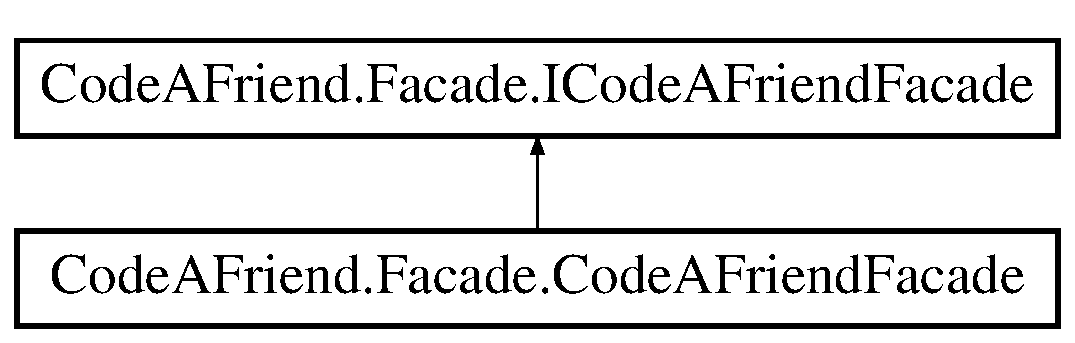
\includegraphics[height=2.000000cm]{interface_code_a_friend_1_1_facade_1_1_i_code_a_friend_facade}
\end{center}
\end{figure}
\subsection*{Public Member Functions}
\begin{DoxyCompactItemize}
\item 
Task$<$ \mbox{\hyperlink{class_code_a_friend_1_1_data_model_1_1_user}{User}} $>$ \mbox{\hyperlink{interface_code_a_friend_1_1_facade_1_1_i_code_a_friend_facade_a2f9f5a0cf07b54b171af4770e519c30b}{Get\+User}} (string username)
\begin{DoxyCompactList}\small\item\em Get a user by their username.\end{DoxyCompactList}\item 
Task$<$ I\+Enumerable$<$ \mbox{\hyperlink{class_code_a_friend_1_1_data_model_1_1_script}{Script}} $>$ $>$ \mbox{\hyperlink{interface_code_a_friend_1_1_facade_1_1_i_code_a_friend_facade_acc0a8e1606ff89320a2cdbcb69f9d338}{Get\+Scripts\+For\+User}} (string username)
\begin{DoxyCompactList}\small\item\em Get all scripts for a user.\end{DoxyCompactList}\item 
Task$<$ \mbox{\hyperlink{class_code_a_friend_1_1_data_model_1_1_script}{Script}} $>$ \mbox{\hyperlink{interface_code_a_friend_1_1_facade_1_1_i_code_a_friend_facade_af180522d16e16c3c7eb69324d87278c0}{Get\+Script\+Async}} (Guid script\+Id)
\begin{DoxyCompactList}\small\item\em Get a user script.\end{DoxyCompactList}\item 
Task$<$ \mbox{\hyperlink{class_code_a_friend_1_1_data_model_1_1_script_evaluation}{Script\+Evaluation}} $>$ \mbox{\hyperlink{interface_code_a_friend_1_1_facade_1_1_i_code_a_friend_facade_abd81f62f5431cd404c9503ff2cfe7e9f}{Execute\+Script\+Async}} (Guid script\+Id, \mbox{\hyperlink{class_code_a_friend_1_1_data_model_1_1_execution_parameters}{Execution\+Parameters}} parameters)
\begin{DoxyCompactList}\small\item\em Execute a user Script with the specified parameters.\end{DoxyCompactList}\item 
Task$<$ I\+Enumerable$<$ \mbox{\hyperlink{class_code_a_friend_1_1_data_model_1_1_script_evaluation}{Script\+Evaluation}} $>$ $>$ \mbox{\hyperlink{interface_code_a_friend_1_1_facade_1_1_i_code_a_friend_facade_a7a3f1a746d41872d14197a8949781ce2}{Execute\+Script\+Async}} (Guid script\+Id, \mbox{\hyperlink{class_code_a_friend_1_1_data_model_1_1_execution_parameters}{Execution\+Parameters}} parameters, params string\mbox{[}$\,$\mbox{]} inputs)
\begin{DoxyCompactList}\small\item\em Execute a Script several times with a specified set of inputs.\end{DoxyCompactList}\item 
Task$<$ T\+Result $>$ \mbox{\hyperlink{interface_code_a_friend_1_1_facade_1_1_i_code_a_friend_facade_a028d0f66e63a4977451e15a0a79c7f19}{Execute\+Command\+Async$<$ T\+Result $>$}} (\mbox{\hyperlink{interface_code_a_friend_1_1_data_model_1_1_i_command}{I\+Command}}$<$ T\+Result $>$ command)
\begin{DoxyCompactList}\small\item\em Execute I\+Command$<$\+T\+Return$>$.\end{DoxyCompactList}\item 
Task$<$ \mbox{\hyperlink{class_code_a_friend_1_1_data_model_1_1_problem}{Problem}} $>$ \mbox{\hyperlink{interface_code_a_friend_1_1_facade_1_1_i_code_a_friend_facade_a044ae5a5e7d55904f0fd43eca50650cb}{Get\+Problem}} (string problem\+Name)
\begin{DoxyCompactList}\small\item\em Get a problem by its name.\end{DoxyCompactList}\end{DoxyCompactItemize}


\subsection{Detailed Description}
Exposes stored user objects for the \mbox{\hyperlink{namespace_code_a_friend}{Code\+A\+Friend}} website. 

Makes use of the facade design pattern.

\subsection{Member Function Documentation}
\mbox{\Hypertarget{interface_code_a_friend_1_1_facade_1_1_i_code_a_friend_facade_a028d0f66e63a4977451e15a0a79c7f19}\label{interface_code_a_friend_1_1_facade_1_1_i_code_a_friend_facade_a028d0f66e63a4977451e15a0a79c7f19}} 
\index{Code\+A\+Friend\+::\+Facade\+::\+I\+Code\+A\+Friend\+Facade@{Code\+A\+Friend\+::\+Facade\+::\+I\+Code\+A\+Friend\+Facade}!Execute\+Command\+Async$<$ T\+Result $>$@{Execute\+Command\+Async$<$ T\+Result $>$}}
\index{Execute\+Command\+Async$<$ T\+Result $>$@{Execute\+Command\+Async$<$ T\+Result $>$}!Code\+A\+Friend\+::\+Facade\+::\+I\+Code\+A\+Friend\+Facade@{Code\+A\+Friend\+::\+Facade\+::\+I\+Code\+A\+Friend\+Facade}}
\subsubsection{\texorpdfstring{Execute\+Command\+Async$<$ T\+Result $>$()}{ExecuteCommandAsync< TResult >()}}
{\footnotesize\ttfamily Task$<$T\+Result$>$ Code\+A\+Friend.\+Facade.\+I\+Code\+A\+Friend\+Facade.\+Execute\+Command\+Async$<$ T\+Result $>$ (\begin{DoxyParamCaption}\item[{\mbox{\hyperlink{interface_code_a_friend_1_1_data_model_1_1_i_command}{I\+Command}}$<$ T\+Result $>$}]{command }\end{DoxyParamCaption})}



Execute I\+Command$<$\+T\+Return$>$.



Implemented in \mbox{\hyperlink{class_code_a_friend_1_1_facade_1_1_code_a_friend_facade_a183e234ee3e7de4e25fb30121dd39891}{Code\+A\+Friend.\+Facade.\+Code\+A\+Friend\+Facade}}.

\mbox{\Hypertarget{interface_code_a_friend_1_1_facade_1_1_i_code_a_friend_facade_abd81f62f5431cd404c9503ff2cfe7e9f}\label{interface_code_a_friend_1_1_facade_1_1_i_code_a_friend_facade_abd81f62f5431cd404c9503ff2cfe7e9f}} 
\index{Code\+A\+Friend\+::\+Facade\+::\+I\+Code\+A\+Friend\+Facade@{Code\+A\+Friend\+::\+Facade\+::\+I\+Code\+A\+Friend\+Facade}!Execute\+Script\+Async@{Execute\+Script\+Async}}
\index{Execute\+Script\+Async@{Execute\+Script\+Async}!Code\+A\+Friend\+::\+Facade\+::\+I\+Code\+A\+Friend\+Facade@{Code\+A\+Friend\+::\+Facade\+::\+I\+Code\+A\+Friend\+Facade}}
\subsubsection{\texorpdfstring{Execute\+Script\+Async()}{ExecuteScriptAsync()}\hspace{0.1cm}{\footnotesize\ttfamily [1/2]}}
{\footnotesize\ttfamily Task$<$\mbox{\hyperlink{class_code_a_friend_1_1_data_model_1_1_script_evaluation}{Script\+Evaluation}}$>$ Code\+A\+Friend.\+Facade.\+I\+Code\+A\+Friend\+Facade.\+Execute\+Script\+Async (\begin{DoxyParamCaption}\item[{Guid}]{script\+Id,  }\item[{\mbox{\hyperlink{class_code_a_friend_1_1_data_model_1_1_execution_parameters}{Execution\+Parameters}}}]{parameters }\end{DoxyParamCaption})}



Execute a user Script with the specified parameters.



Implemented in \mbox{\hyperlink{class_code_a_friend_1_1_facade_1_1_code_a_friend_facade_a04883cd14eb596a9f9113c24aa06e34b}{Code\+A\+Friend.\+Facade.\+Code\+A\+Friend\+Facade}}.

\mbox{\Hypertarget{interface_code_a_friend_1_1_facade_1_1_i_code_a_friend_facade_a7a3f1a746d41872d14197a8949781ce2}\label{interface_code_a_friend_1_1_facade_1_1_i_code_a_friend_facade_a7a3f1a746d41872d14197a8949781ce2}} 
\index{Code\+A\+Friend\+::\+Facade\+::\+I\+Code\+A\+Friend\+Facade@{Code\+A\+Friend\+::\+Facade\+::\+I\+Code\+A\+Friend\+Facade}!Execute\+Script\+Async@{Execute\+Script\+Async}}
\index{Execute\+Script\+Async@{Execute\+Script\+Async}!Code\+A\+Friend\+::\+Facade\+::\+I\+Code\+A\+Friend\+Facade@{Code\+A\+Friend\+::\+Facade\+::\+I\+Code\+A\+Friend\+Facade}}
\subsubsection{\texorpdfstring{Execute\+Script\+Async()}{ExecuteScriptAsync()}\hspace{0.1cm}{\footnotesize\ttfamily [2/2]}}
{\footnotesize\ttfamily Task$<$I\+Enumerable$<$\mbox{\hyperlink{class_code_a_friend_1_1_data_model_1_1_script_evaluation}{Script\+Evaluation}}$>$ $>$ Code\+A\+Friend.\+Facade.\+I\+Code\+A\+Friend\+Facade.\+Execute\+Script\+Async (\begin{DoxyParamCaption}\item[{Guid}]{script\+Id,  }\item[{\mbox{\hyperlink{class_code_a_friend_1_1_data_model_1_1_execution_parameters}{Execution\+Parameters}}}]{parameters,  }\item[{params string \mbox{[}$\,$\mbox{]}}]{inputs }\end{DoxyParamCaption})}



Execute a Script several times with a specified set of inputs.



Implemented in \mbox{\hyperlink{class_code_a_friend_1_1_facade_1_1_code_a_friend_facade_abcd7e13b8e5a7accbcd56b4f7eee8934}{Code\+A\+Friend.\+Facade.\+Code\+A\+Friend\+Facade}}.

\mbox{\Hypertarget{interface_code_a_friend_1_1_facade_1_1_i_code_a_friend_facade_a044ae5a5e7d55904f0fd43eca50650cb}\label{interface_code_a_friend_1_1_facade_1_1_i_code_a_friend_facade_a044ae5a5e7d55904f0fd43eca50650cb}} 
\index{Code\+A\+Friend\+::\+Facade\+::\+I\+Code\+A\+Friend\+Facade@{Code\+A\+Friend\+::\+Facade\+::\+I\+Code\+A\+Friend\+Facade}!Get\+Problem@{Get\+Problem}}
\index{Get\+Problem@{Get\+Problem}!Code\+A\+Friend\+::\+Facade\+::\+I\+Code\+A\+Friend\+Facade@{Code\+A\+Friend\+::\+Facade\+::\+I\+Code\+A\+Friend\+Facade}}
\subsubsection{\texorpdfstring{Get\+Problem()}{GetProblem()}}
{\footnotesize\ttfamily Task$<$\mbox{\hyperlink{class_code_a_friend_1_1_data_model_1_1_problem}{Problem}}$>$ Code\+A\+Friend.\+Facade.\+I\+Code\+A\+Friend\+Facade.\+Get\+Problem (\begin{DoxyParamCaption}\item[{string}]{problem\+Name }\end{DoxyParamCaption})}



Get a problem by its name.



Implemented in \mbox{\hyperlink{class_code_a_friend_1_1_facade_1_1_code_a_friend_facade_a0fd5153f295a66388ef6a6d4880f32bd}{Code\+A\+Friend.\+Facade.\+Code\+A\+Friend\+Facade}}.

\mbox{\Hypertarget{interface_code_a_friend_1_1_facade_1_1_i_code_a_friend_facade_af180522d16e16c3c7eb69324d87278c0}\label{interface_code_a_friend_1_1_facade_1_1_i_code_a_friend_facade_af180522d16e16c3c7eb69324d87278c0}} 
\index{Code\+A\+Friend\+::\+Facade\+::\+I\+Code\+A\+Friend\+Facade@{Code\+A\+Friend\+::\+Facade\+::\+I\+Code\+A\+Friend\+Facade}!Get\+Script\+Async@{Get\+Script\+Async}}
\index{Get\+Script\+Async@{Get\+Script\+Async}!Code\+A\+Friend\+::\+Facade\+::\+I\+Code\+A\+Friend\+Facade@{Code\+A\+Friend\+::\+Facade\+::\+I\+Code\+A\+Friend\+Facade}}
\subsubsection{\texorpdfstring{Get\+Script\+Async()}{GetScriptAsync()}}
{\footnotesize\ttfamily Task$<$\mbox{\hyperlink{class_code_a_friend_1_1_data_model_1_1_script}{Script}}$>$ Code\+A\+Friend.\+Facade.\+I\+Code\+A\+Friend\+Facade.\+Get\+Script\+Async (\begin{DoxyParamCaption}\item[{Guid}]{script\+Id }\end{DoxyParamCaption})}



Get a user script.



Implemented in \mbox{\hyperlink{class_code_a_friend_1_1_facade_1_1_code_a_friend_facade_aaf0ac4c19567b0078140ab3d6a457e15}{Code\+A\+Friend.\+Facade.\+Code\+A\+Friend\+Facade}}.

\mbox{\Hypertarget{interface_code_a_friend_1_1_facade_1_1_i_code_a_friend_facade_acc0a8e1606ff89320a2cdbcb69f9d338}\label{interface_code_a_friend_1_1_facade_1_1_i_code_a_friend_facade_acc0a8e1606ff89320a2cdbcb69f9d338}} 
\index{Code\+A\+Friend\+::\+Facade\+::\+I\+Code\+A\+Friend\+Facade@{Code\+A\+Friend\+::\+Facade\+::\+I\+Code\+A\+Friend\+Facade}!Get\+Scripts\+For\+User@{Get\+Scripts\+For\+User}}
\index{Get\+Scripts\+For\+User@{Get\+Scripts\+For\+User}!Code\+A\+Friend\+::\+Facade\+::\+I\+Code\+A\+Friend\+Facade@{Code\+A\+Friend\+::\+Facade\+::\+I\+Code\+A\+Friend\+Facade}}
\subsubsection{\texorpdfstring{Get\+Scripts\+For\+User()}{GetScriptsForUser()}}
{\footnotesize\ttfamily Task$<$I\+Enumerable$<$\mbox{\hyperlink{class_code_a_friend_1_1_data_model_1_1_script}{Script}}$>$ $>$ Code\+A\+Friend.\+Facade.\+I\+Code\+A\+Friend\+Facade.\+Get\+Scripts\+For\+User (\begin{DoxyParamCaption}\item[{string}]{username }\end{DoxyParamCaption})}



Get all scripts for a user.



Implemented in \mbox{\hyperlink{class_code_a_friend_1_1_facade_1_1_code_a_friend_facade_a77cd5040946e3a1feaac9fc03cfdb372}{Code\+A\+Friend.\+Facade.\+Code\+A\+Friend\+Facade}}.

\mbox{\Hypertarget{interface_code_a_friend_1_1_facade_1_1_i_code_a_friend_facade_a2f9f5a0cf07b54b171af4770e519c30b}\label{interface_code_a_friend_1_1_facade_1_1_i_code_a_friend_facade_a2f9f5a0cf07b54b171af4770e519c30b}} 
\index{Code\+A\+Friend\+::\+Facade\+::\+I\+Code\+A\+Friend\+Facade@{Code\+A\+Friend\+::\+Facade\+::\+I\+Code\+A\+Friend\+Facade}!Get\+User@{Get\+User}}
\index{Get\+User@{Get\+User}!Code\+A\+Friend\+::\+Facade\+::\+I\+Code\+A\+Friend\+Facade@{Code\+A\+Friend\+::\+Facade\+::\+I\+Code\+A\+Friend\+Facade}}
\subsubsection{\texorpdfstring{Get\+User()}{GetUser()}}
{\footnotesize\ttfamily Task$<$\mbox{\hyperlink{class_code_a_friend_1_1_data_model_1_1_user}{User}}$>$ Code\+A\+Friend.\+Facade.\+I\+Code\+A\+Friend\+Facade.\+Get\+User (\begin{DoxyParamCaption}\item[{string}]{username }\end{DoxyParamCaption})}



Get a user by their username.



Implemented in \mbox{\hyperlink{class_code_a_friend_1_1_facade_1_1_code_a_friend_facade_a5cc08aa0377f29fd3f80e1d880059951}{Code\+A\+Friend.\+Facade.\+Code\+A\+Friend\+Facade}}.



The documentation for this interface was generated from the following file\+:\begin{DoxyCompactItemize}
\item 
shared/\+Code\+A\+Friend.\+Facade/\mbox{\hyperlink{_i_code_a_friend_facade_8cs}{I\+Code\+A\+Friend\+Facade.\+cs}}\end{DoxyCompactItemize}

\hypertarget{interface_code_a_friend_1_1_data_model_1_1_i_command}{}\section{Code\+A\+Friend.\+Data\+Model.\+I\+Command$<$ T\+Return $>$ Interface Template Reference}
\label{interface_code_a_friend_1_1_data_model_1_1_i_command}\index{Code\+A\+Friend.\+Data\+Model.\+I\+Command$<$ T\+Return $>$@{Code\+A\+Friend.\+Data\+Model.\+I\+Command$<$ T\+Return $>$}}


An operation to perform on the \mbox{\hyperlink{namespace_code_a_friend}{Code\+A\+Friend}} backend.  


\subsection*{Public Member Functions}
\begin{DoxyCompactItemize}
\item 
Task$<$ T\+Return $>$ \mbox{\hyperlink{interface_code_a_friend_1_1_data_model_1_1_i_command_a203b6d77d611382df2e9a8961a3bccaa}{Execute\+Async}} (Db\+Context context)
\begin{DoxyCompactList}\small\item\em Asynchronously execute this command and return the resulting {\itshape T\+Return} . \end{DoxyCompactList}\end{DoxyCompactItemize}


\subsection{Detailed Description}
An operation to perform on the \mbox{\hyperlink{namespace_code_a_friend}{Code\+A\+Friend}} backend. 


\begin{DoxyTemplParams}{Template Parameters}
{\em T\+Return} & Type that will be returned by the execute.\\
\hline
\end{DoxyTemplParams}


\subsection{Member Function Documentation}
\mbox{\Hypertarget{interface_code_a_friend_1_1_data_model_1_1_i_command_a203b6d77d611382df2e9a8961a3bccaa}\label{interface_code_a_friend_1_1_data_model_1_1_i_command_a203b6d77d611382df2e9a8961a3bccaa}} 
\index{Code\+A\+Friend\+::\+Data\+Model\+::\+I\+Command@{Code\+A\+Friend\+::\+Data\+Model\+::\+I\+Command}!Execute\+Async@{Execute\+Async}}
\index{Execute\+Async@{Execute\+Async}!Code\+A\+Friend\+::\+Data\+Model\+::\+I\+Command@{Code\+A\+Friend\+::\+Data\+Model\+::\+I\+Command}}
\subsubsection{\texorpdfstring{Execute\+Async()}{ExecuteAsync()}}
{\footnotesize\ttfamily Task$<$T\+Return$>$ \mbox{\hyperlink{interface_code_a_friend_1_1_data_model_1_1_i_command}{Code\+A\+Friend.\+Data\+Model.\+I\+Command}}$<$ T\+Return $>$.Execute\+Async (\begin{DoxyParamCaption}\item[{Db\+Context}]{context }\end{DoxyParamCaption})}



Asynchronously execute this command and return the resulting {\itshape T\+Return} . 

\begin{DoxyReturn}{Returns}

\end{DoxyReturn}


The documentation for this interface was generated from the following file\+:\begin{DoxyCompactItemize}
\item 
shared/\+Code\+A\+Friend.\+Data\+Model/\mbox{\hyperlink{_i_command_8cs}{I\+Command.\+cs}}\end{DoxyCompactItemize}

\hypertarget{interface_code_a_friend_1_1_languages_1_1_core_1_1_i_interpreter_factory}{}\section{Code\+A\+Friend.\+Languages.\+Core.\+I\+Interpreter\+Factory Interface Reference}
\label{interface_code_a_friend_1_1_languages_1_1_core_1_1_i_interpreter_factory}\index{Code\+A\+Friend.\+Languages.\+Core.\+I\+Interpreter\+Factory@{Code\+A\+Friend.\+Languages.\+Core.\+I\+Interpreter\+Factory}}


Factory to get the proper interpreter given a supplied language  


Inheritance diagram for Code\+A\+Friend.\+Languages.\+Core.\+I\+Interpreter\+Factory\+:\begin{figure}[H]
\begin{center}
\leavevmode
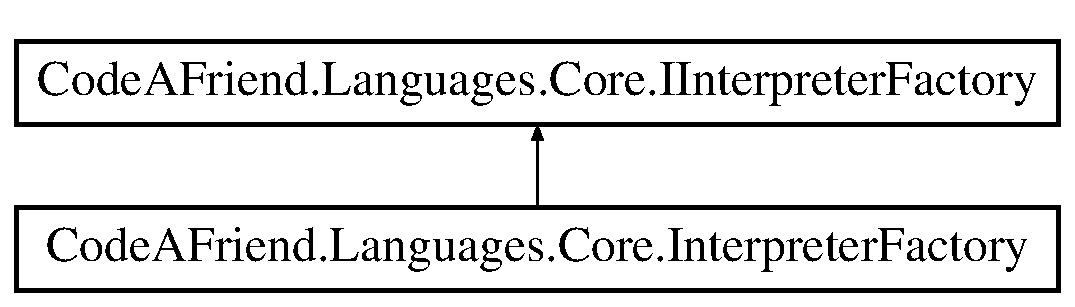
\includegraphics[height=2.000000cm]{interface_code_a_friend_1_1_languages_1_1_core_1_1_i_interpreter_factory}
\end{center}
\end{figure}
\subsection*{Public Member Functions}
\begin{DoxyCompactItemize}
\item 
\mbox{\hyperlink{interface_code_a_friend_1_1_data_model_1_1_i_language_interpreter}{I\+Language\+Interpreter}} \mbox{\hyperlink{interface_code_a_friend_1_1_languages_1_1_core_1_1_i_interpreter_factory_a4d2f3ae695515fc3c28f352a20bfd601}{Get\+Interpreter}} (\mbox{\hyperlink{namespace_code_a_friend_1_1_data_model_a13e088c525db1b03a4de75420ced79b2}{Supported\+Language}} language)
\begin{DoxyCompactList}\small\item\em Get an appropriate I\+Language\+Interpreter. \end{DoxyCompactList}\end{DoxyCompactItemize}


\subsection{Detailed Description}
Factory to get the proper interpreter given a supplied language 



\subsection{Member Function Documentation}
\mbox{\Hypertarget{interface_code_a_friend_1_1_languages_1_1_core_1_1_i_interpreter_factory_a4d2f3ae695515fc3c28f352a20bfd601}\label{interface_code_a_friend_1_1_languages_1_1_core_1_1_i_interpreter_factory_a4d2f3ae695515fc3c28f352a20bfd601}} 
\index{Code\+A\+Friend\+::\+Languages\+::\+Core\+::\+I\+Interpreter\+Factory@{Code\+A\+Friend\+::\+Languages\+::\+Core\+::\+I\+Interpreter\+Factory}!Get\+Interpreter@{Get\+Interpreter}}
\index{Get\+Interpreter@{Get\+Interpreter}!Code\+A\+Friend\+::\+Languages\+::\+Core\+::\+I\+Interpreter\+Factory@{Code\+A\+Friend\+::\+Languages\+::\+Core\+::\+I\+Interpreter\+Factory}}
\subsubsection{\texorpdfstring{Get\+Interpreter()}{GetInterpreter()}}
{\footnotesize\ttfamily \mbox{\hyperlink{interface_code_a_friend_1_1_data_model_1_1_i_language_interpreter}{I\+Language\+Interpreter}} Code\+A\+Friend.\+Languages.\+Core.\+I\+Interpreter\+Factory.\+Get\+Interpreter (\begin{DoxyParamCaption}\item[{\mbox{\hyperlink{namespace_code_a_friend_1_1_data_model_a13e088c525db1b03a4de75420ced79b2}{Supported\+Language}}}]{language }\end{DoxyParamCaption})}



Get an appropriate I\+Language\+Interpreter. 


\begin{DoxyParams}{Parameters}
{\em language} & Language to grab I\+Language\+Interpreter for.\\
\hline
\end{DoxyParams}
\begin{DoxyReturn}{Returns}
Appropriate I\+Language\+Interpreter.
\end{DoxyReturn}


Implemented in \mbox{\hyperlink{class_code_a_friend_1_1_languages_1_1_core_1_1_interpreter_factory_ac39dea6ec4f5612ecf3ab49a920fc543}{Code\+A\+Friend.\+Languages.\+Core.\+Interpreter\+Factory}}.



The documentation for this interface was generated from the following file\+:\begin{DoxyCompactItemize}
\item 
shared/\+Code\+A\+Friend.\+Languages.\+Core/\mbox{\hyperlink{_i_interpreter_factory_8cs}{I\+Interpreter\+Factory.\+cs}}\end{DoxyCompactItemize}

\hypertarget{interface_code_a_friend_1_1_data_model_1_1_i_language_interpreter}{}\section{Code\+A\+Friend.\+Data\+Model.\+I\+Language\+Interpreter Interface Reference}
\label{interface_code_a_friend_1_1_data_model_1_1_i_language_interpreter}\index{Code\+A\+Friend.\+Data\+Model.\+I\+Language\+Interpreter@{Code\+A\+Friend.\+Data\+Model.\+I\+Language\+Interpreter}}


Exposes the ability to compile and execute a specific language.  


Inheritance diagram for Code\+A\+Friend.\+Data\+Model.\+I\+Language\+Interpreter\+:\begin{figure}[H]
\begin{center}
\leavevmode
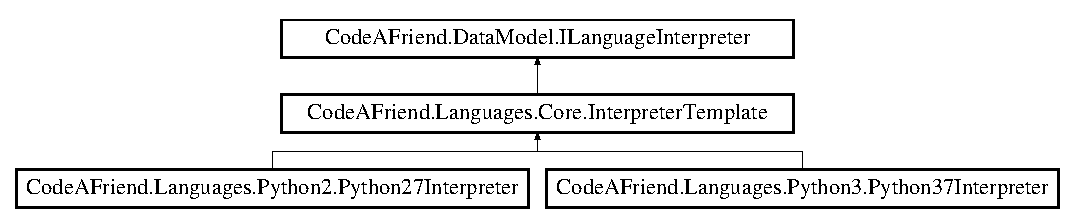
\includegraphics[height=2.560976cm]{interface_code_a_friend_1_1_data_model_1_1_i_language_interpreter}
\end{center}
\end{figure}
\subsection*{Public Member Functions}
\begin{DoxyCompactItemize}
\item 
Task$<$ \mbox{\hyperlink{class_code_a_friend_1_1_data_model_1_1_script_evaluation}{Script\+Evaluation}} $>$ \mbox{\hyperlink{interface_code_a_friend_1_1_data_model_1_1_i_language_interpreter_a3003897aaa13ee672b6157c584e46898}{Execute\+Async}} (string body, \mbox{\hyperlink{class_code_a_friend_1_1_data_model_1_1_execution_parameters}{Execution\+Parameters}} parameters)
\begin{DoxyCompactList}\small\item\em Execute code written in \mbox{\hyperlink{interface_code_a_friend_1_1_data_model_1_1_i_language_interpreter_ab8d4ee55278929fb59f3f015789aaa36}{Name}} language using the specified \mbox{\hyperlink{class_code_a_friend_1_1_data_model_1_1_execution_parameters}{Execution\+Parameters}}. \end{DoxyCompactList}\end{DoxyCompactItemize}
\subsection*{Properties}
\begin{DoxyCompactItemize}
\item 
\mbox{\hyperlink{namespace_code_a_friend_1_1_data_model_a13e088c525db1b03a4de75420ced79b2}{Supported\+Language}} \mbox{\hyperlink{interface_code_a_friend_1_1_data_model_1_1_i_language_interpreter_ab8d4ee55278929fb59f3f015789aaa36}{Name}}\hspace{0.3cm}{\ttfamily  \mbox{[}get\mbox{]}}
\begin{DoxyCompactList}\small\item\em The language this \mbox{\hyperlink{interface_code_a_friend_1_1_data_model_1_1_i_language_interpreter}{I\+Language\+Interpreter}} interprets. \end{DoxyCompactList}\end{DoxyCompactItemize}


\subsection{Detailed Description}
Exposes the ability to compile and execute a specific language. 



\subsection{Member Function Documentation}
\mbox{\Hypertarget{interface_code_a_friend_1_1_data_model_1_1_i_language_interpreter_a3003897aaa13ee672b6157c584e46898}\label{interface_code_a_friend_1_1_data_model_1_1_i_language_interpreter_a3003897aaa13ee672b6157c584e46898}} 
\index{Code\+A\+Friend\+::\+Data\+Model\+::\+I\+Language\+Interpreter@{Code\+A\+Friend\+::\+Data\+Model\+::\+I\+Language\+Interpreter}!Execute\+Async@{Execute\+Async}}
\index{Execute\+Async@{Execute\+Async}!Code\+A\+Friend\+::\+Data\+Model\+::\+I\+Language\+Interpreter@{Code\+A\+Friend\+::\+Data\+Model\+::\+I\+Language\+Interpreter}}
\subsubsection{\texorpdfstring{Execute\+Async()}{ExecuteAsync()}}
{\footnotesize\ttfamily Task$<$\mbox{\hyperlink{class_code_a_friend_1_1_data_model_1_1_script_evaluation}{Script\+Evaluation}}$>$ Code\+A\+Friend.\+Data\+Model.\+I\+Language\+Interpreter.\+Execute\+Async (\begin{DoxyParamCaption}\item[{string}]{body,  }\item[{\mbox{\hyperlink{class_code_a_friend_1_1_data_model_1_1_execution_parameters}{Execution\+Parameters}}}]{parameters }\end{DoxyParamCaption})}



Execute code written in \mbox{\hyperlink{interface_code_a_friend_1_1_data_model_1_1_i_language_interpreter_ab8d4ee55278929fb59f3f015789aaa36}{Name}} language using the specified \mbox{\hyperlink{class_code_a_friend_1_1_data_model_1_1_execution_parameters}{Execution\+Parameters}}. 


\begin{DoxyParams}{Parameters}
{\em body} & \\
\hline
{\em parameters} & The \mbox{\hyperlink{class_code_a_friend_1_1_data_model_1_1_execution_parameters}{Execution\+Parameters}} to use for code compilation and execution.\\
\hline
\end{DoxyParams}
\begin{DoxyReturn}{Returns}
\mbox{\hyperlink{class_code_a_friend_1_1_data_model_1_1_script_evaluation}{Script\+Evaluation}}
\end{DoxyReturn}


Implemented in \mbox{\hyperlink{class_code_a_friend_1_1_languages_1_1_core_1_1_interpreter_template_ae2cf761e61f7b6b6fc553703ea3ba3c5}{Code\+A\+Friend.\+Languages.\+Core.\+Interpreter\+Template}}.



\subsection{Property Documentation}
\mbox{\Hypertarget{interface_code_a_friend_1_1_data_model_1_1_i_language_interpreter_ab8d4ee55278929fb59f3f015789aaa36}\label{interface_code_a_friend_1_1_data_model_1_1_i_language_interpreter_ab8d4ee55278929fb59f3f015789aaa36}} 
\index{Code\+A\+Friend\+::\+Data\+Model\+::\+I\+Language\+Interpreter@{Code\+A\+Friend\+::\+Data\+Model\+::\+I\+Language\+Interpreter}!Name@{Name}}
\index{Name@{Name}!Code\+A\+Friend\+::\+Data\+Model\+::\+I\+Language\+Interpreter@{Code\+A\+Friend\+::\+Data\+Model\+::\+I\+Language\+Interpreter}}
\subsubsection{\texorpdfstring{Name}{Name}}
{\footnotesize\ttfamily \mbox{\hyperlink{namespace_code_a_friend_1_1_data_model_a13e088c525db1b03a4de75420ced79b2}{Supported\+Language}} Code\+A\+Friend.\+Data\+Model.\+I\+Language\+Interpreter.\+Name\hspace{0.3cm}{\ttfamily [get]}}



The language this \mbox{\hyperlink{interface_code_a_friend_1_1_data_model_1_1_i_language_interpreter}{I\+Language\+Interpreter}} interprets. 



The documentation for this interface was generated from the following file\+:\begin{DoxyCompactItemize}
\item 
shared/\+Code\+A\+Friend.\+Data\+Model/\+Script\+Logic/\mbox{\hyperlink{_i_language_interpreter_8cs}{I\+Language\+Interpreter.\+cs}}\end{DoxyCompactItemize}

\hypertarget{class_code_a_friend_1_1_repository_1_1_migrations_1_1_initial_create}{}\section{Code\+A\+Friend.\+Repository.\+Migrations.\+Initial\+Create Class Reference}
\label{class_code_a_friend_1_1_repository_1_1_migrations_1_1_initial_create}\index{Code\+A\+Friend.\+Repository.\+Migrations.\+Initial\+Create@{Code\+A\+Friend.\+Repository.\+Migrations.\+Initial\+Create}}
Inheritance diagram for Code\+A\+Friend.\+Repository.\+Migrations.\+Initial\+Create\+:\begin{figure}[H]
\begin{center}
\leavevmode
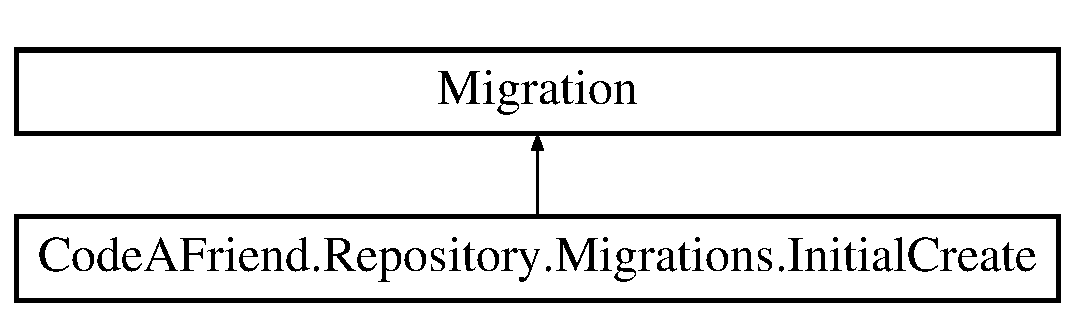
\includegraphics[height=2.000000cm]{class_code_a_friend_1_1_repository_1_1_migrations_1_1_initial_create}
\end{center}
\end{figure}
\subsection*{Protected Member Functions}
\begin{DoxyCompactItemize}
\item 
override void \mbox{\hyperlink{class_code_a_friend_1_1_repository_1_1_migrations_1_1_initial_create_a74096fd245fe8053636da0e6b42555f5}{Up}} (Migration\+Builder migration\+Builder)
\item 
override void \mbox{\hyperlink{class_code_a_friend_1_1_repository_1_1_migrations_1_1_initial_create_a990a4291d83d80015cb2f085f32d3e2a}{Down}} (Migration\+Builder migration\+Builder)
\item 
override void \mbox{\hyperlink{class_code_a_friend_1_1_repository_1_1_migrations_1_1_initial_create_af61ca20b8cd6530bcd97d1d9d238cac2}{Build\+Target\+Model}} (Model\+Builder model\+Builder)
\end{DoxyCompactItemize}


\subsection{Member Function Documentation}
\mbox{\Hypertarget{class_code_a_friend_1_1_repository_1_1_migrations_1_1_initial_create_af61ca20b8cd6530bcd97d1d9d238cac2}\label{class_code_a_friend_1_1_repository_1_1_migrations_1_1_initial_create_af61ca20b8cd6530bcd97d1d9d238cac2}} 
\index{Code\+A\+Friend\+::\+Repository\+::\+Migrations\+::\+Initial\+Create@{Code\+A\+Friend\+::\+Repository\+::\+Migrations\+::\+Initial\+Create}!Build\+Target\+Model@{Build\+Target\+Model}}
\index{Build\+Target\+Model@{Build\+Target\+Model}!Code\+A\+Friend\+::\+Repository\+::\+Migrations\+::\+Initial\+Create@{Code\+A\+Friend\+::\+Repository\+::\+Migrations\+::\+Initial\+Create}}
\subsubsection{\texorpdfstring{Build\+Target\+Model()}{BuildTargetModel()}}
{\footnotesize\ttfamily override void Code\+A\+Friend.\+Repository.\+Migrations.\+Initial\+Create.\+Build\+Target\+Model (\begin{DoxyParamCaption}\item[{Model\+Builder}]{model\+Builder }\end{DoxyParamCaption})\hspace{0.3cm}{\ttfamily [protected]}}

\mbox{\Hypertarget{class_code_a_friend_1_1_repository_1_1_migrations_1_1_initial_create_a990a4291d83d80015cb2f085f32d3e2a}\label{class_code_a_friend_1_1_repository_1_1_migrations_1_1_initial_create_a990a4291d83d80015cb2f085f32d3e2a}} 
\index{Code\+A\+Friend\+::\+Repository\+::\+Migrations\+::\+Initial\+Create@{Code\+A\+Friend\+::\+Repository\+::\+Migrations\+::\+Initial\+Create}!Down@{Down}}
\index{Down@{Down}!Code\+A\+Friend\+::\+Repository\+::\+Migrations\+::\+Initial\+Create@{Code\+A\+Friend\+::\+Repository\+::\+Migrations\+::\+Initial\+Create}}
\subsubsection{\texorpdfstring{Down()}{Down()}}
{\footnotesize\ttfamily override void Code\+A\+Friend.\+Repository.\+Migrations.\+Initial\+Create.\+Down (\begin{DoxyParamCaption}\item[{Migration\+Builder}]{migration\+Builder }\end{DoxyParamCaption})\hspace{0.3cm}{\ttfamily [protected]}}

\mbox{\Hypertarget{class_code_a_friend_1_1_repository_1_1_migrations_1_1_initial_create_a74096fd245fe8053636da0e6b42555f5}\label{class_code_a_friend_1_1_repository_1_1_migrations_1_1_initial_create_a74096fd245fe8053636da0e6b42555f5}} 
\index{Code\+A\+Friend\+::\+Repository\+::\+Migrations\+::\+Initial\+Create@{Code\+A\+Friend\+::\+Repository\+::\+Migrations\+::\+Initial\+Create}!Up@{Up}}
\index{Up@{Up}!Code\+A\+Friend\+::\+Repository\+::\+Migrations\+::\+Initial\+Create@{Code\+A\+Friend\+::\+Repository\+::\+Migrations\+::\+Initial\+Create}}
\subsubsection{\texorpdfstring{Up()}{Up()}}
{\footnotesize\ttfamily override void Code\+A\+Friend.\+Repository.\+Migrations.\+Initial\+Create.\+Up (\begin{DoxyParamCaption}\item[{Migration\+Builder}]{migration\+Builder }\end{DoxyParamCaption})\hspace{0.3cm}{\ttfamily [protected]}}



The documentation for this class was generated from the following files\+:\begin{DoxyCompactItemize}
\item 
shared/\+Code\+A\+Friend.\+Repository/\+Migrations/\mbox{\hyperlink{20181118213026___initial_create_8cs}{20181118213026\+\_\+\+Initial\+Create.\+cs}}\item 
shared/\+Code\+A\+Friend.\+Repository/\+Migrations/\mbox{\hyperlink{20181118213026___initial_create_8_designer_8cs}{20181118213026\+\_\+\+Initial\+Create.\+Designer.\+cs}}\end{DoxyCompactItemize}

\hypertarget{class_code_a_friend_1_1_languages_1_1_core_1_1_interpreter_factory}{}\section{Code\+A\+Friend.\+Languages.\+Core.\+Interpreter\+Factory Class Reference}
\label{class_code_a_friend_1_1_languages_1_1_core_1_1_interpreter_factory}\index{Code\+A\+Friend.\+Languages.\+Core.\+Interpreter\+Factory@{Code\+A\+Friend.\+Languages.\+Core.\+Interpreter\+Factory}}
Inheritance diagram for Code\+A\+Friend.\+Languages.\+Core.\+Interpreter\+Factory\+:\begin{figure}[H]
\begin{center}
\leavevmode
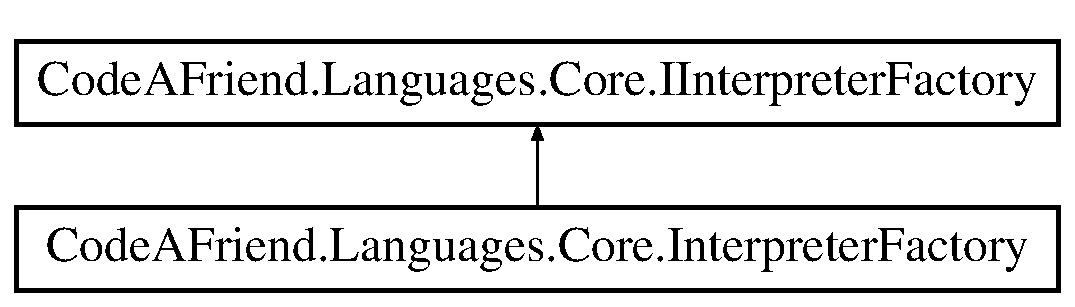
\includegraphics[height=2.000000cm]{class_code_a_friend_1_1_languages_1_1_core_1_1_interpreter_factory}
\end{center}
\end{figure}
\subsection*{Public Member Functions}
\begin{DoxyCompactItemize}
\item 
\mbox{\hyperlink{class_code_a_friend_1_1_languages_1_1_core_1_1_interpreter_factory_ae86fb2de2ee28532b67d0e89fcd7bcbb}{Interpreter\+Factory}} (I\+Memory\+Cache cache)
\begin{DoxyCompactList}\small\item\em DI constructor.\end{DoxyCompactList}\item 
\mbox{\hyperlink{interface_code_a_friend_1_1_data_model_1_1_i_language_interpreter}{I\+Language\+Interpreter}} \mbox{\hyperlink{class_code_a_friend_1_1_languages_1_1_core_1_1_interpreter_factory_ac39dea6ec4f5612ecf3ab49a920fc543}{Get\+Interpreter}} (\mbox{\hyperlink{namespace_code_a_friend_1_1_data_model_a13e088c525db1b03a4de75420ced79b2}{Supported\+Language}} language)
\begin{DoxyCompactList}\small\item\em Get an appropriate I\+Language\+Interpreter.  \end{DoxyCompactList}\end{DoxyCompactItemize}


\subsection{Detailed Description}
Uses a cache where appropriate.

\subsection{Constructor \& Destructor Documentation}
\mbox{\Hypertarget{class_code_a_friend_1_1_languages_1_1_core_1_1_interpreter_factory_ae86fb2de2ee28532b67d0e89fcd7bcbb}\label{class_code_a_friend_1_1_languages_1_1_core_1_1_interpreter_factory_ae86fb2de2ee28532b67d0e89fcd7bcbb}} 
\index{Code\+A\+Friend\+::\+Languages\+::\+Core\+::\+Interpreter\+Factory@{Code\+A\+Friend\+::\+Languages\+::\+Core\+::\+Interpreter\+Factory}!Interpreter\+Factory@{Interpreter\+Factory}}
\index{Interpreter\+Factory@{Interpreter\+Factory}!Code\+A\+Friend\+::\+Languages\+::\+Core\+::\+Interpreter\+Factory@{Code\+A\+Friend\+::\+Languages\+::\+Core\+::\+Interpreter\+Factory}}
\subsubsection{\texorpdfstring{Interpreter\+Factory()}{InterpreterFactory()}}
{\footnotesize\ttfamily Code\+A\+Friend.\+Languages.\+Core.\+Interpreter\+Factory.\+Interpreter\+Factory (\begin{DoxyParamCaption}\item[{I\+Memory\+Cache}]{cache }\end{DoxyParamCaption})}



DI constructor.



\subsection{Member Function Documentation}
\mbox{\Hypertarget{class_code_a_friend_1_1_languages_1_1_core_1_1_interpreter_factory_ac39dea6ec4f5612ecf3ab49a920fc543}\label{class_code_a_friend_1_1_languages_1_1_core_1_1_interpreter_factory_ac39dea6ec4f5612ecf3ab49a920fc543}} 
\index{Code\+A\+Friend\+::\+Languages\+::\+Core\+::\+Interpreter\+Factory@{Code\+A\+Friend\+::\+Languages\+::\+Core\+::\+Interpreter\+Factory}!Get\+Interpreter@{Get\+Interpreter}}
\index{Get\+Interpreter@{Get\+Interpreter}!Code\+A\+Friend\+::\+Languages\+::\+Core\+::\+Interpreter\+Factory@{Code\+A\+Friend\+::\+Languages\+::\+Core\+::\+Interpreter\+Factory}}
\subsubsection{\texorpdfstring{Get\+Interpreter()}{GetInterpreter()}}
{\footnotesize\ttfamily \mbox{\hyperlink{interface_code_a_friend_1_1_data_model_1_1_i_language_interpreter}{I\+Language\+Interpreter}} Code\+A\+Friend.\+Languages.\+Core.\+Interpreter\+Factory.\+Get\+Interpreter (\begin{DoxyParamCaption}\item[{\mbox{\hyperlink{namespace_code_a_friend_1_1_data_model_a13e088c525db1b03a4de75420ced79b2}{Supported\+Language}}}]{language }\end{DoxyParamCaption})}



Get an appropriate I\+Language\+Interpreter.  



Implements \mbox{\hyperlink{interface_code_a_friend_1_1_languages_1_1_core_1_1_i_interpreter_factory_a4d2f3ae695515fc3c28f352a20bfd601}{Code\+A\+Friend.\+Languages.\+Core.\+I\+Interpreter\+Factory}}.



The documentation for this class was generated from the following file\+:\begin{DoxyCompactItemize}
\item 
shared/\+Code\+A\+Friend.\+Languages.\+Factory/\mbox{\hyperlink{_interpreter_factory_8cs}{Interpreter\+Factory.\+cs}}\end{DoxyCompactItemize}

\hypertarget{class_code_a_friend_1_1_languages_1_1_core_1_1_interpreter_template}{}\section{Code\+A\+Friend.\+Languages.\+Core.\+Interpreter\+Template Class Reference}
\label{class_code_a_friend_1_1_languages_1_1_core_1_1_interpreter_template}\index{Code\+A\+Friend.\+Languages.\+Core.\+Interpreter\+Template@{Code\+A\+Friend.\+Languages.\+Core.\+Interpreter\+Template}}
Inheritance diagram for Code\+A\+Friend.\+Languages.\+Core.\+Interpreter\+Template\+:\begin{figure}[H]
\begin{center}
\leavevmode
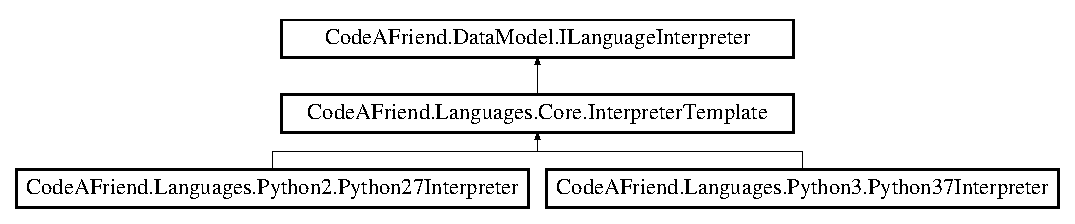
\includegraphics[height=2.560976cm]{class_code_a_friend_1_1_languages_1_1_core_1_1_interpreter_template}
\end{center}
\end{figure}
\subsection*{Public Member Functions}
\begin{DoxyCompactItemize}
\item 
async Task$<$ \mbox{\hyperlink{class_code_a_friend_1_1_data_model_1_1_script_evaluation}{Script\+Evaluation}} $>$ \mbox{\hyperlink{class_code_a_friend_1_1_languages_1_1_core_1_1_interpreter_template_ae2cf761e61f7b6b6fc553703ea3ba3c5}{Execute\+Async}} (string body, \mbox{\hyperlink{class_code_a_friend_1_1_data_model_1_1_execution_parameters}{Execution\+Parameters}} parameters)
\begin{DoxyCompactList}\small\item\em Execute code written in \mbox{\hyperlink{interface_code_a_friend_1_1_data_model_1_1_i_language_interpreter_ab8d4ee55278929fb59f3f015789aaa36}{Name}} language using the specified \mbox{\hyperlink{class_code_a_friend_1_1_data_model_1_1_execution_parameters}{Execution\+Parameters}}.  \end{DoxyCompactList}\item 
virtual async Task$<$ string $>$ \mbox{\hyperlink{class_code_a_friend_1_1_languages_1_1_core_1_1_interpreter_template_aedeed04eb6f14cb6bec2a9f250b71ebb}{Write\+Script\+To\+File\+Async}} (string script\+Body)
\item 
abstract Process\+Start\+Info \mbox{\hyperlink{class_code_a_friend_1_1_languages_1_1_core_1_1_interpreter_template_a2f8560fba2e22a9cdf22c8d2f7bb849f}{Get\+Process\+Start\+Info}} (string script\+File\+Path)
\item 
virtual async Task$<$ \mbox{\hyperlink{class_code_a_friend_1_1_data_model_1_1_script_evaluation}{Script\+Evaluation}} $>$ \mbox{\hyperlink{class_code_a_friend_1_1_languages_1_1_core_1_1_interpreter_template_aa76d5e57b00dfa82862362288d140e1b}{Run\+Process\+Async}} (\mbox{\hyperlink{class_code_a_friend_1_1_data_model_1_1_execution_parameters}{Execution\+Parameters}} parameters, Process\+Start\+Info start\+Info, string script\+File\+Path)
\end{DoxyCompactItemize}
\subsection*{Properties}
\begin{DoxyCompactItemize}
\item 
abstract \mbox{\hyperlink{namespace_code_a_friend_1_1_data_model_a13e088c525db1b03a4de75420ced79b2}{Supported\+Language}} \mbox{\hyperlink{class_code_a_friend_1_1_languages_1_1_core_1_1_interpreter_template_a7c5eeadd02916f2e314f3290d1dbdc8c}{Name}}\hspace{0.3cm}{\ttfamily  \mbox{[}get\mbox{]}}
\end{DoxyCompactItemize}


\subsection{Member Function Documentation}
\mbox{\Hypertarget{class_code_a_friend_1_1_languages_1_1_core_1_1_interpreter_template_ae2cf761e61f7b6b6fc553703ea3ba3c5}\label{class_code_a_friend_1_1_languages_1_1_core_1_1_interpreter_template_ae2cf761e61f7b6b6fc553703ea3ba3c5}} 
\index{Code\+A\+Friend\+::\+Languages\+::\+Core\+::\+Interpreter\+Template@{Code\+A\+Friend\+::\+Languages\+::\+Core\+::\+Interpreter\+Template}!Execute\+Async@{Execute\+Async}}
\index{Execute\+Async@{Execute\+Async}!Code\+A\+Friend\+::\+Languages\+::\+Core\+::\+Interpreter\+Template@{Code\+A\+Friend\+::\+Languages\+::\+Core\+::\+Interpreter\+Template}}
\subsubsection{\texorpdfstring{Execute\+Async()}{ExecuteAsync()}}
{\footnotesize\ttfamily async Task$<$\mbox{\hyperlink{class_code_a_friend_1_1_data_model_1_1_script_evaluation}{Script\+Evaluation}}$>$ Code\+A\+Friend.\+Languages.\+Core.\+Interpreter\+Template.\+Execute\+Async (\begin{DoxyParamCaption}\item[{string}]{body,  }\item[{\mbox{\hyperlink{class_code_a_friend_1_1_data_model_1_1_execution_parameters}{Execution\+Parameters}}}]{parameters }\end{DoxyParamCaption})}



Execute code written in \mbox{\hyperlink{interface_code_a_friend_1_1_data_model_1_1_i_language_interpreter_ab8d4ee55278929fb59f3f015789aaa36}{Name}} language using the specified \mbox{\hyperlink{class_code_a_friend_1_1_data_model_1_1_execution_parameters}{Execution\+Parameters}}.  



Implements \mbox{\hyperlink{interface_code_a_friend_1_1_data_model_1_1_i_language_interpreter_a3003897aaa13ee672b6157c584e46898}{Code\+A\+Friend.\+Data\+Model.\+I\+Language\+Interpreter}}.

\mbox{\Hypertarget{class_code_a_friend_1_1_languages_1_1_core_1_1_interpreter_template_a2f8560fba2e22a9cdf22c8d2f7bb849f}\label{class_code_a_friend_1_1_languages_1_1_core_1_1_interpreter_template_a2f8560fba2e22a9cdf22c8d2f7bb849f}} 
\index{Code\+A\+Friend\+::\+Languages\+::\+Core\+::\+Interpreter\+Template@{Code\+A\+Friend\+::\+Languages\+::\+Core\+::\+Interpreter\+Template}!Get\+Process\+Start\+Info@{Get\+Process\+Start\+Info}}
\index{Get\+Process\+Start\+Info@{Get\+Process\+Start\+Info}!Code\+A\+Friend\+::\+Languages\+::\+Core\+::\+Interpreter\+Template@{Code\+A\+Friend\+::\+Languages\+::\+Core\+::\+Interpreter\+Template}}
\subsubsection{\texorpdfstring{Get\+Process\+Start\+Info()}{GetProcessStartInfo()}}
{\footnotesize\ttfamily abstract Process\+Start\+Info Code\+A\+Friend.\+Languages.\+Core.\+Interpreter\+Template.\+Get\+Process\+Start\+Info (\begin{DoxyParamCaption}\item[{string}]{script\+File\+Path }\end{DoxyParamCaption})\hspace{0.3cm}{\ttfamily [pure virtual]}}



Implemented in \mbox{\hyperlink{class_code_a_friend_1_1_languages_1_1_python2_1_1_python27_interpreter_a24b4f1f296ab282b0fcac3951af0a73b}{Code\+A\+Friend.\+Languages.\+Python2.\+Python27\+Interpreter}}, and \mbox{\hyperlink{class_code_a_friend_1_1_languages_1_1_python3_1_1_python37_interpreter_a61f777c41849f97cd94eccee5fe7c617}{Code\+A\+Friend.\+Languages.\+Python3.\+Python37\+Interpreter}}.

\mbox{\Hypertarget{class_code_a_friend_1_1_languages_1_1_core_1_1_interpreter_template_aa76d5e57b00dfa82862362288d140e1b}\label{class_code_a_friend_1_1_languages_1_1_core_1_1_interpreter_template_aa76d5e57b00dfa82862362288d140e1b}} 
\index{Code\+A\+Friend\+::\+Languages\+::\+Core\+::\+Interpreter\+Template@{Code\+A\+Friend\+::\+Languages\+::\+Core\+::\+Interpreter\+Template}!Run\+Process\+Async@{Run\+Process\+Async}}
\index{Run\+Process\+Async@{Run\+Process\+Async}!Code\+A\+Friend\+::\+Languages\+::\+Core\+::\+Interpreter\+Template@{Code\+A\+Friend\+::\+Languages\+::\+Core\+::\+Interpreter\+Template}}
\subsubsection{\texorpdfstring{Run\+Process\+Async()}{RunProcessAsync()}}
{\footnotesize\ttfamily virtual async Task$<$\mbox{\hyperlink{class_code_a_friend_1_1_data_model_1_1_script_evaluation}{Script\+Evaluation}}$>$ Code\+A\+Friend.\+Languages.\+Core.\+Interpreter\+Template.\+Run\+Process\+Async (\begin{DoxyParamCaption}\item[{\mbox{\hyperlink{class_code_a_friend_1_1_data_model_1_1_execution_parameters}{Execution\+Parameters}}}]{parameters,  }\item[{Process\+Start\+Info}]{start\+Info,  }\item[{string}]{script\+File\+Path }\end{DoxyParamCaption})\hspace{0.3cm}{\ttfamily [virtual]}}

\mbox{\Hypertarget{class_code_a_friend_1_1_languages_1_1_core_1_1_interpreter_template_aedeed04eb6f14cb6bec2a9f250b71ebb}\label{class_code_a_friend_1_1_languages_1_1_core_1_1_interpreter_template_aedeed04eb6f14cb6bec2a9f250b71ebb}} 
\index{Code\+A\+Friend\+::\+Languages\+::\+Core\+::\+Interpreter\+Template@{Code\+A\+Friend\+::\+Languages\+::\+Core\+::\+Interpreter\+Template}!Write\+Script\+To\+File\+Async@{Write\+Script\+To\+File\+Async}}
\index{Write\+Script\+To\+File\+Async@{Write\+Script\+To\+File\+Async}!Code\+A\+Friend\+::\+Languages\+::\+Core\+::\+Interpreter\+Template@{Code\+A\+Friend\+::\+Languages\+::\+Core\+::\+Interpreter\+Template}}
\subsubsection{\texorpdfstring{Write\+Script\+To\+File\+Async()}{WriteScriptToFileAsync()}}
{\footnotesize\ttfamily virtual async Task$<$string$>$ Code\+A\+Friend.\+Languages.\+Core.\+Interpreter\+Template.\+Write\+Script\+To\+File\+Async (\begin{DoxyParamCaption}\item[{string}]{script\+Body }\end{DoxyParamCaption})\hspace{0.3cm}{\ttfamily [virtual]}}



\subsection{Property Documentation}
\mbox{\Hypertarget{class_code_a_friend_1_1_languages_1_1_core_1_1_interpreter_template_a7c5eeadd02916f2e314f3290d1dbdc8c}\label{class_code_a_friend_1_1_languages_1_1_core_1_1_interpreter_template_a7c5eeadd02916f2e314f3290d1dbdc8c}} 
\index{Code\+A\+Friend\+::\+Languages\+::\+Core\+::\+Interpreter\+Template@{Code\+A\+Friend\+::\+Languages\+::\+Core\+::\+Interpreter\+Template}!Name@{Name}}
\index{Name@{Name}!Code\+A\+Friend\+::\+Languages\+::\+Core\+::\+Interpreter\+Template@{Code\+A\+Friend\+::\+Languages\+::\+Core\+::\+Interpreter\+Template}}
\subsubsection{\texorpdfstring{Name}{Name}}
{\footnotesize\ttfamily abstract \mbox{\hyperlink{namespace_code_a_friend_1_1_data_model_a13e088c525db1b03a4de75420ced79b2}{Supported\+Language}} Code\+A\+Friend.\+Languages.\+Core.\+Interpreter\+Template.\+Name\hspace{0.3cm}{\ttfamily [get]}}







The documentation for this class was generated from the following file\+:\begin{DoxyCompactItemize}
\item 
shared/\+Code\+A\+Friend.\+Languages.\+Core/\mbox{\hyperlink{_interpreter_template_8cs}{Interpreter\+Template.\+cs}}\end{DoxyCompactItemize}

\hypertarget{class_code_a_friend_1_1_data_model_1_1_problem}{}\section{Code\+A\+Friend.\+Data\+Model.\+Problem Class Reference}
\label{class_code_a_friend_1_1_data_model_1_1_problem}\index{Code\+A\+Friend.\+Data\+Model.\+Problem@{Code\+A\+Friend.\+Data\+Model.\+Problem}}


A problem with a set of \mbox{\hyperlink{class_code_a_friend_1_1_data_model_1_1_test_case}{Test\+Case}}s to determine if a \mbox{\hyperlink{class_code_a_friend_1_1_data_model_1_1_script}{Script}} solves the \mbox{\hyperlink{class_code_a_friend_1_1_data_model_1_1_problem}{Problem}}.  


\subsection*{Public Member Functions}
\begin{DoxyCompactItemize}
\item 
\mbox{\hyperlink{class_code_a_friend_1_1_data_model_1_1_problem_a0bd8bd69a5f4d301be856222262fe7fc}{Problem}} (string name, string description, \mbox{\hyperlink{class_code_a_friend_1_1_data_model_1_1_user}{User}} user)
\begin{DoxyCompactList}\small\item\em Constructor for creating new \mbox{\hyperlink{class_code_a_friend_1_1_data_model_1_1_problem}{Problem}}.\end{DoxyCompactList}\item 
async Task$<$ bool $>$ \mbox{\hyperlink{class_code_a_friend_1_1_data_model_1_1_problem_a9b792cd3ea05e6efcd351cf138d06516}{Test\+Script}} (\mbox{\hyperlink{class_code_a_friend_1_1_data_model_1_1_script}{Script}} script, \mbox{\hyperlink{interface_code_a_friend_1_1_data_model_1_1_i_language_interpreter}{I\+Language\+Interpreter}} interpreter)
\begin{DoxyCompactList}\small\item\em Test if a script is a \mbox{\hyperlink{class_code_a_friend_1_1_data_model_1_1_problem_solution}{Problem\+Solution}}. \end{DoxyCompactList}\item 
void \mbox{\hyperlink{class_code_a_friend_1_1_data_model_1_1_problem_a3ca779158ac6d2f5ca49206214722d27}{Add}} (\mbox{\hyperlink{class_code_a_friend_1_1_data_model_1_1_test_case}{Test\+Case}} test\+Case, Db\+Context context=null)
\begin{DoxyCompactList}\small\item\em Add a \mbox{\hyperlink{class_code_a_friend_1_1_data_model_1_1_test_case}{Test\+Case}} to this \mbox{\hyperlink{class_code_a_friend_1_1_data_model_1_1_problem}{Problem}}. \end{DoxyCompactList}\item 
void \mbox{\hyperlink{class_code_a_friend_1_1_data_model_1_1_problem_a72e426e2924615d8fc813de8303bc16b}{Add}} (\mbox{\hyperlink{class_code_a_friend_1_1_data_model_1_1_problem_solution}{Problem\+Solution}} solution, Db\+Context context=null)
\begin{DoxyCompactList}\small\item\em Add a \mbox{\hyperlink{class_code_a_friend_1_1_data_model_1_1_problem_solution}{Problem\+Solution}} to this \mbox{\hyperlink{class_code_a_friend_1_1_data_model_1_1_problem}{Problem}}. \end{DoxyCompactList}\item 
void \mbox{\hyperlink{class_code_a_friend_1_1_data_model_1_1_problem_ab8ba911fa018638164edf5fe6d0076ec}{Add}} (\mbox{\hyperlink{class_code_a_friend_1_1_data_model_1_1_tag}{Tag}} tag, Db\+Context context=null)
\begin{DoxyCompactList}\small\item\em Add a \mbox{\hyperlink{class_code_a_friend_1_1_data_model_1_1_tag}{Tag}} to this \mbox{\hyperlink{class_code_a_friend_1_1_data_model_1_1_problem}{Problem}}. \end{DoxyCompactList}\end{DoxyCompactItemize}
\subsection*{Public Attributes}
\begin{DoxyCompactItemize}
\item 
virtual I\+Enumerable$<$ \mbox{\hyperlink{class_code_a_friend_1_1_data_model_1_1_test_case}{Test\+Case}} $>$ \mbox{\hyperlink{class_code_a_friend_1_1_data_model_1_1_problem_af4a665cdf0e4349c57e8588e95ad9717}{Test\+Cases}} =$>$ \+\_\+test\+Cases?.To\+List()
\begin{DoxyCompactList}\small\item\em \mbox{\hyperlink{class_code_a_friend_1_1_data_model_1_1_test_case}{Test\+Case}}s for this problem.\end{DoxyCompactList}\item 
virtual I\+Enumerable$<$ \mbox{\hyperlink{class_code_a_friend_1_1_data_model_1_1_problem_solution}{Problem\+Solution}} $>$ \mbox{\hyperlink{class_code_a_friend_1_1_data_model_1_1_problem_a3bebdf4e45042e9476fd7ae7cf38738b}{Solutions}} =$>$ \+\_\+solutions?.To\+List()
\begin{DoxyCompactList}\small\item\em \mbox{\hyperlink{class_code_a_friend_1_1_data_model_1_1_script}{Script}}s that passed all \mbox{\hyperlink{class_code_a_friend_1_1_data_model_1_1_problem_af4a665cdf0e4349c57e8588e95ad9717}{Test\+Cases}}.\end{DoxyCompactList}\item 
virtual I\+Enumerable$<$ \mbox{\hyperlink{class_code_a_friend_1_1_data_model_1_1_tag}{Tag}} $>$ \mbox{\hyperlink{class_code_a_friend_1_1_data_model_1_1_problem_ad5c3e1b321171d7c7723df70e99cf88d}{Tags}} =$>$ \+\_\+tags?.To\+List()
\begin{DoxyCompactList}\small\item\em Optional tags to use to search for this problem.\end{DoxyCompactList}\end{DoxyCompactItemize}
\subsection*{Properties}
\begin{DoxyCompactItemize}
\item 
virtual string \mbox{\hyperlink{class_code_a_friend_1_1_data_model_1_1_problem_a32bbc148bbaffc060632720e2ab860fb}{Name}}\hspace{0.3cm}{\ttfamily  \mbox{[}get\mbox{]}}
\begin{DoxyCompactList}\small\item\em Unique name of the \mbox{\hyperlink{class_code_a_friend_1_1_data_model_1_1_problem}{Problem}}.\end{DoxyCompactList}\item 
virtual string \mbox{\hyperlink{class_code_a_friend_1_1_data_model_1_1_problem_a62094d748f4eed72d44f25bdab3047dc}{Description}}\hspace{0.3cm}{\ttfamily  \mbox{[}get\mbox{]}}
\begin{DoxyCompactList}\small\item\em Description of this \mbox{\hyperlink{class_code_a_friend_1_1_data_model_1_1_problem}{Problem}}.\end{DoxyCompactList}\item 
virtual \mbox{\hyperlink{class_code_a_friend_1_1_data_model_1_1_user}{User}} \mbox{\hyperlink{class_code_a_friend_1_1_data_model_1_1_problem_a16adf7da62fca6b430006e5d0c099c96}{User}}\hspace{0.3cm}{\ttfamily  \mbox{[}get\mbox{]}}
\begin{DoxyCompactList}\small\item\em \mbox{\hyperlink{class_code_a_friend_1_1_data_model_1_1_user}{User}} who submitted this \mbox{\hyperlink{class_code_a_friend_1_1_data_model_1_1_problem}{Problem}}.\end{DoxyCompactList}\end{DoxyCompactItemize}


\subsection{Detailed Description}
A problem with a set of \mbox{\hyperlink{class_code_a_friend_1_1_data_model_1_1_test_case}{Test\+Case}}s to determine if a \mbox{\hyperlink{class_code_a_friend_1_1_data_model_1_1_script}{Script}} solves the \mbox{\hyperlink{class_code_a_friend_1_1_data_model_1_1_problem}{Problem}}. 



\subsection{Constructor \& Destructor Documentation}
\mbox{\Hypertarget{class_code_a_friend_1_1_data_model_1_1_problem_a0bd8bd69a5f4d301be856222262fe7fc}\label{class_code_a_friend_1_1_data_model_1_1_problem_a0bd8bd69a5f4d301be856222262fe7fc}} 
\index{Code\+A\+Friend\+::\+Data\+Model\+::\+Problem@{Code\+A\+Friend\+::\+Data\+Model\+::\+Problem}!Problem@{Problem}}
\index{Problem@{Problem}!Code\+A\+Friend\+::\+Data\+Model\+::\+Problem@{Code\+A\+Friend\+::\+Data\+Model\+::\+Problem}}
\subsubsection{\texorpdfstring{Problem()}{Problem()}}
{\footnotesize\ttfamily Code\+A\+Friend.\+Data\+Model.\+Problem.\+Problem (\begin{DoxyParamCaption}\item[{string}]{name,  }\item[{string}]{description,  }\item[{\mbox{\hyperlink{class_code_a_friend_1_1_data_model_1_1_user}{User}}}]{user }\end{DoxyParamCaption})}



Constructor for creating new \mbox{\hyperlink{class_code_a_friend_1_1_data_model_1_1_problem}{Problem}}.



\subsection{Member Function Documentation}
\mbox{\Hypertarget{class_code_a_friend_1_1_data_model_1_1_problem_a3ca779158ac6d2f5ca49206214722d27}\label{class_code_a_friend_1_1_data_model_1_1_problem_a3ca779158ac6d2f5ca49206214722d27}} 
\index{Code\+A\+Friend\+::\+Data\+Model\+::\+Problem@{Code\+A\+Friend\+::\+Data\+Model\+::\+Problem}!Add@{Add}}
\index{Add@{Add}!Code\+A\+Friend\+::\+Data\+Model\+::\+Problem@{Code\+A\+Friend\+::\+Data\+Model\+::\+Problem}}
\subsubsection{\texorpdfstring{Add()}{Add()}\hspace{0.1cm}{\footnotesize\ttfamily [1/3]}}
{\footnotesize\ttfamily void Code\+A\+Friend.\+Data\+Model.\+Problem.\+Add (\begin{DoxyParamCaption}\item[{\mbox{\hyperlink{class_code_a_friend_1_1_data_model_1_1_test_case}{Test\+Case}}}]{test\+Case,  }\item[{Db\+Context}]{context = {\ttfamily null} }\end{DoxyParamCaption})}



Add a \mbox{\hyperlink{class_code_a_friend_1_1_data_model_1_1_test_case}{Test\+Case}} to this \mbox{\hyperlink{class_code_a_friend_1_1_data_model_1_1_problem}{Problem}}. 


\begin{DoxyParams}{Parameters}
{\em test\+Case} & \mbox{\hyperlink{class_code_a_friend_1_1_data_model_1_1_test_case}{Test\+Case}} to add.\\
\hline
{\em context} & Database to save the updated state to. (When Save\+Changes is called).\\
\hline
\end{DoxyParams}
\mbox{\Hypertarget{class_code_a_friend_1_1_data_model_1_1_problem_a72e426e2924615d8fc813de8303bc16b}\label{class_code_a_friend_1_1_data_model_1_1_problem_a72e426e2924615d8fc813de8303bc16b}} 
\index{Code\+A\+Friend\+::\+Data\+Model\+::\+Problem@{Code\+A\+Friend\+::\+Data\+Model\+::\+Problem}!Add@{Add}}
\index{Add@{Add}!Code\+A\+Friend\+::\+Data\+Model\+::\+Problem@{Code\+A\+Friend\+::\+Data\+Model\+::\+Problem}}
\subsubsection{\texorpdfstring{Add()}{Add()}\hspace{0.1cm}{\footnotesize\ttfamily [2/3]}}
{\footnotesize\ttfamily void Code\+A\+Friend.\+Data\+Model.\+Problem.\+Add (\begin{DoxyParamCaption}\item[{\mbox{\hyperlink{class_code_a_friend_1_1_data_model_1_1_problem_solution}{Problem\+Solution}}}]{solution,  }\item[{Db\+Context}]{context = {\ttfamily null} }\end{DoxyParamCaption})}



Add a \mbox{\hyperlink{class_code_a_friend_1_1_data_model_1_1_problem_solution}{Problem\+Solution}} to this \mbox{\hyperlink{class_code_a_friend_1_1_data_model_1_1_problem}{Problem}}. 


\begin{DoxyParams}{Parameters}
{\em solution} & \mbox{\hyperlink{class_code_a_friend_1_1_data_model_1_1_problem_solution}{Problem\+Solution}} to add.\\
\hline
{\em context} & Database to save the updated state to. (When Save\+Changes is called).\\
\hline
\end{DoxyParams}
\mbox{\Hypertarget{class_code_a_friend_1_1_data_model_1_1_problem_ab8ba911fa018638164edf5fe6d0076ec}\label{class_code_a_friend_1_1_data_model_1_1_problem_ab8ba911fa018638164edf5fe6d0076ec}} 
\index{Code\+A\+Friend\+::\+Data\+Model\+::\+Problem@{Code\+A\+Friend\+::\+Data\+Model\+::\+Problem}!Add@{Add}}
\index{Add@{Add}!Code\+A\+Friend\+::\+Data\+Model\+::\+Problem@{Code\+A\+Friend\+::\+Data\+Model\+::\+Problem}}
\subsubsection{\texorpdfstring{Add()}{Add()}\hspace{0.1cm}{\footnotesize\ttfamily [3/3]}}
{\footnotesize\ttfamily void Code\+A\+Friend.\+Data\+Model.\+Problem.\+Add (\begin{DoxyParamCaption}\item[{\mbox{\hyperlink{class_code_a_friend_1_1_data_model_1_1_tag}{Tag}}}]{tag,  }\item[{Db\+Context}]{context = {\ttfamily null} }\end{DoxyParamCaption})}



Add a \mbox{\hyperlink{class_code_a_friend_1_1_data_model_1_1_tag}{Tag}} to this \mbox{\hyperlink{class_code_a_friend_1_1_data_model_1_1_problem}{Problem}}. 


\begin{DoxyParams}{Parameters}
{\em tag} & \mbox{\hyperlink{class_code_a_friend_1_1_data_model_1_1_tag}{Tag}} to add.\\
\hline
{\em context} & Database to save the updated state to. (When Save\+Changes is called).\\
\hline
\end{DoxyParams}
\mbox{\Hypertarget{class_code_a_friend_1_1_data_model_1_1_problem_a9b792cd3ea05e6efcd351cf138d06516}\label{class_code_a_friend_1_1_data_model_1_1_problem_a9b792cd3ea05e6efcd351cf138d06516}} 
\index{Code\+A\+Friend\+::\+Data\+Model\+::\+Problem@{Code\+A\+Friend\+::\+Data\+Model\+::\+Problem}!Test\+Script@{Test\+Script}}
\index{Test\+Script@{Test\+Script}!Code\+A\+Friend\+::\+Data\+Model\+::\+Problem@{Code\+A\+Friend\+::\+Data\+Model\+::\+Problem}}
\subsubsection{\texorpdfstring{Test\+Script()}{TestScript()}}
{\footnotesize\ttfamily async Task$<$bool$>$ Code\+A\+Friend.\+Data\+Model.\+Problem.\+Test\+Script (\begin{DoxyParamCaption}\item[{\mbox{\hyperlink{class_code_a_friend_1_1_data_model_1_1_script}{Script}}}]{script,  }\item[{\mbox{\hyperlink{interface_code_a_friend_1_1_data_model_1_1_i_language_interpreter}{I\+Language\+Interpreter}}}]{interpreter }\end{DoxyParamCaption})}



Test if a script is a \mbox{\hyperlink{class_code_a_friend_1_1_data_model_1_1_problem_solution}{Problem\+Solution}}. 


\begin{DoxyParams}{Parameters}
{\em script} & \mbox{\hyperlink{class_code_a_friend_1_1_data_model_1_1_script}{Script}} to run.\\
\hline
{\em interpreter} & \\
\hline
\end{DoxyParams}
\begin{DoxyReturn}{Returns}
bool
\end{DoxyReturn}


\subsection{Member Data Documentation}
\mbox{\Hypertarget{class_code_a_friend_1_1_data_model_1_1_problem_a3bebdf4e45042e9476fd7ae7cf38738b}\label{class_code_a_friend_1_1_data_model_1_1_problem_a3bebdf4e45042e9476fd7ae7cf38738b}} 
\index{Code\+A\+Friend\+::\+Data\+Model\+::\+Problem@{Code\+A\+Friend\+::\+Data\+Model\+::\+Problem}!Solutions@{Solutions}}
\index{Solutions@{Solutions}!Code\+A\+Friend\+::\+Data\+Model\+::\+Problem@{Code\+A\+Friend\+::\+Data\+Model\+::\+Problem}}
\subsubsection{\texorpdfstring{Solutions}{Solutions}}
{\footnotesize\ttfamily virtual I\+Enumerable$<$\mbox{\hyperlink{class_code_a_friend_1_1_data_model_1_1_problem_solution}{Problem\+Solution}}$>$ Code\+A\+Friend.\+Data\+Model.\+Problem.\+Solutions =$>$ \+\_\+solutions?.To\+List()}



\mbox{\hyperlink{class_code_a_friend_1_1_data_model_1_1_script}{Script}}s that passed all \mbox{\hyperlink{class_code_a_friend_1_1_data_model_1_1_problem_af4a665cdf0e4349c57e8588e95ad9717}{Test\+Cases}}.

\mbox{\Hypertarget{class_code_a_friend_1_1_data_model_1_1_problem_ad5c3e1b321171d7c7723df70e99cf88d}\label{class_code_a_friend_1_1_data_model_1_1_problem_ad5c3e1b321171d7c7723df70e99cf88d}} 
\index{Code\+A\+Friend\+::\+Data\+Model\+::\+Problem@{Code\+A\+Friend\+::\+Data\+Model\+::\+Problem}!Tags@{Tags}}
\index{Tags@{Tags}!Code\+A\+Friend\+::\+Data\+Model\+::\+Problem@{Code\+A\+Friend\+::\+Data\+Model\+::\+Problem}}
\subsubsection{\texorpdfstring{Tags}{Tags}}
{\footnotesize\ttfamily virtual I\+Enumerable$<$\mbox{\hyperlink{class_code_a_friend_1_1_data_model_1_1_tag}{Tag}}$>$ Code\+A\+Friend.\+Data\+Model.\+Problem.\+Tags =$>$ \+\_\+tags?.To\+List()}



Optional tags to use to search for this problem.

\mbox{\Hypertarget{class_code_a_friend_1_1_data_model_1_1_problem_af4a665cdf0e4349c57e8588e95ad9717}\label{class_code_a_friend_1_1_data_model_1_1_problem_af4a665cdf0e4349c57e8588e95ad9717}} 
\index{Code\+A\+Friend\+::\+Data\+Model\+::\+Problem@{Code\+A\+Friend\+::\+Data\+Model\+::\+Problem}!Test\+Cases@{Test\+Cases}}
\index{Test\+Cases@{Test\+Cases}!Code\+A\+Friend\+::\+Data\+Model\+::\+Problem@{Code\+A\+Friend\+::\+Data\+Model\+::\+Problem}}
\subsubsection{\texorpdfstring{Test\+Cases}{TestCases}}
{\footnotesize\ttfamily virtual I\+Enumerable$<$\mbox{\hyperlink{class_code_a_friend_1_1_data_model_1_1_test_case}{Test\+Case}}$>$ Code\+A\+Friend.\+Data\+Model.\+Problem.\+Test\+Cases =$>$ \+\_\+test\+Cases?.To\+List()}



\mbox{\hyperlink{class_code_a_friend_1_1_data_model_1_1_test_case}{Test\+Case}}s for this problem.



\subsection{Property Documentation}
\mbox{\Hypertarget{class_code_a_friend_1_1_data_model_1_1_problem_a62094d748f4eed72d44f25bdab3047dc}\label{class_code_a_friend_1_1_data_model_1_1_problem_a62094d748f4eed72d44f25bdab3047dc}} 
\index{Code\+A\+Friend\+::\+Data\+Model\+::\+Problem@{Code\+A\+Friend\+::\+Data\+Model\+::\+Problem}!Description@{Description}}
\index{Description@{Description}!Code\+A\+Friend\+::\+Data\+Model\+::\+Problem@{Code\+A\+Friend\+::\+Data\+Model\+::\+Problem}}
\subsubsection{\texorpdfstring{Description}{Description}}
{\footnotesize\ttfamily virtual string Code\+A\+Friend.\+Data\+Model.\+Problem.\+Description\hspace{0.3cm}{\ttfamily [get]}}



Description of this \mbox{\hyperlink{class_code_a_friend_1_1_data_model_1_1_problem}{Problem}}.

\mbox{\Hypertarget{class_code_a_friend_1_1_data_model_1_1_problem_a32bbc148bbaffc060632720e2ab860fb}\label{class_code_a_friend_1_1_data_model_1_1_problem_a32bbc148bbaffc060632720e2ab860fb}} 
\index{Code\+A\+Friend\+::\+Data\+Model\+::\+Problem@{Code\+A\+Friend\+::\+Data\+Model\+::\+Problem}!Name@{Name}}
\index{Name@{Name}!Code\+A\+Friend\+::\+Data\+Model\+::\+Problem@{Code\+A\+Friend\+::\+Data\+Model\+::\+Problem}}
\subsubsection{\texorpdfstring{Name}{Name}}
{\footnotesize\ttfamily virtual string Code\+A\+Friend.\+Data\+Model.\+Problem.\+Name\hspace{0.3cm}{\ttfamily [get]}}



Unique name of the \mbox{\hyperlink{class_code_a_friend_1_1_data_model_1_1_problem}{Problem}}.

\mbox{\Hypertarget{class_code_a_friend_1_1_data_model_1_1_problem_a16adf7da62fca6b430006e5d0c099c96}\label{class_code_a_friend_1_1_data_model_1_1_problem_a16adf7da62fca6b430006e5d0c099c96}} 
\index{Code\+A\+Friend\+::\+Data\+Model\+::\+Problem@{Code\+A\+Friend\+::\+Data\+Model\+::\+Problem}!User@{User}}
\index{User@{User}!Code\+A\+Friend\+::\+Data\+Model\+::\+Problem@{Code\+A\+Friend\+::\+Data\+Model\+::\+Problem}}
\subsubsection{\texorpdfstring{User}{User}}
{\footnotesize\ttfamily virtual \mbox{\hyperlink{class_code_a_friend_1_1_data_model_1_1_user}{User}} Code\+A\+Friend.\+Data\+Model.\+Problem.\+User\hspace{0.3cm}{\ttfamily [get]}}



\mbox{\hyperlink{class_code_a_friend_1_1_data_model_1_1_user}{User}} who submitted this \mbox{\hyperlink{class_code_a_friend_1_1_data_model_1_1_problem}{Problem}}.



The documentation for this class was generated from the following file\+:\begin{DoxyCompactItemize}
\item 
shared/\+Code\+A\+Friend.\+Data\+Model/\+Problem\+Logic/\mbox{\hyperlink{_problem_8cs}{Problem.\+cs}}\end{DoxyCompactItemize}

\hypertarget{class_code_a_friend_1_1_api_service_1_1_controllers_1_1_problem_controller}{}\section{Code\+A\+Friend.\+Api\+Service.\+Controllers.\+Problem\+Controller Class Reference}
\label{class_code_a_friend_1_1_api_service_1_1_controllers_1_1_problem_controller}\index{Code\+A\+Friend.\+Api\+Service.\+Controllers.\+Problem\+Controller@{Code\+A\+Friend.\+Api\+Service.\+Controllers.\+Problem\+Controller}}


Api Methods dealing with Problems.  


Inheritance diagram for Code\+A\+Friend.\+Api\+Service.\+Controllers.\+Problem\+Controller\+:\begin{figure}[H]
\begin{center}
\leavevmode
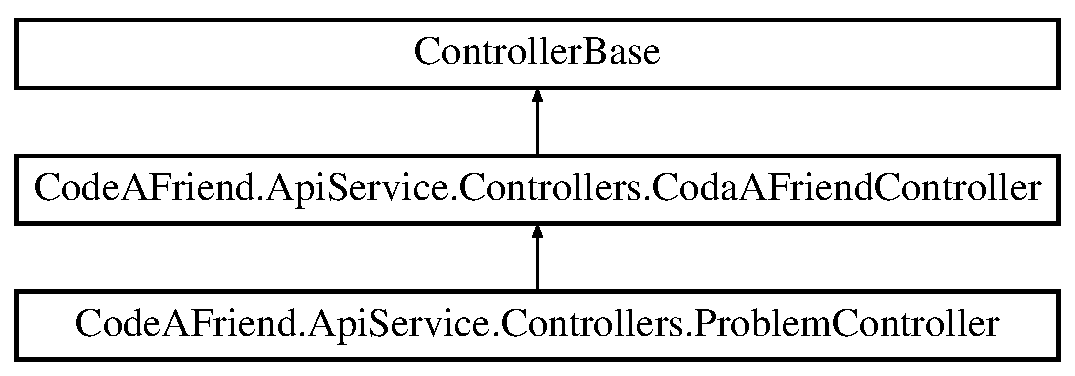
\includegraphics[height=3.000000cm]{class_code_a_friend_1_1_api_service_1_1_controllers_1_1_problem_controller}
\end{center}
\end{figure}
\subsection*{Public Member Functions}
\begin{DoxyCompactItemize}
\item 
\mbox{\hyperlink{class_code_a_friend_1_1_api_service_1_1_controllers_1_1_problem_controller_a2f0d98d308a3adc0712b52b4fd3945de}{Problem\+Controller}} (\mbox{\hyperlink{interface_code_a_friend_1_1_facade_1_1_i_code_a_friend_facade}{I\+Code\+A\+Friend\+Facade}} facade)
\item 
async Task$<$ I\+Action\+Result $>$ \mbox{\hyperlink{class_code_a_friend_1_1_api_service_1_1_controllers_1_1_problem_controller_a9f87dcfa7186b6ea75f2ac690a06cdbe}{Add\+Problem\+For\+User}} (\mbox{\hyperlink{class_code_a_friend_1_1_data_model_1_1_user_1_1_add_problem_command}{User.\+Add\+Problem\+Command}} command)
\begin{DoxyCompactList}\small\item\em Create the specified Problem. \end{DoxyCompactList}\item 
async Task$<$ I\+Action\+Result $>$ \mbox{\hyperlink{class_code_a_friend_1_1_api_service_1_1_controllers_1_1_problem_controller_a3ae37d2a578e67e48c1b1a91894c61b0}{Update\+Problem}} (\mbox{\hyperlink{class_code_a_friend_1_1_data_model_1_1_user_1_1_update_problem_command}{User.\+Update\+Problem\+Command}} command)
\begin{DoxyCompactList}\small\item\em Update the specified Problem. \end{DoxyCompactList}\item 
async Task$<$ I\+Action\+Result $>$ \mbox{\hyperlink{class_code_a_friend_1_1_api_service_1_1_controllers_1_1_problem_controller_a2b8c284c32ccf82a763ee27a349d72b3}{Delete\+Problem}} (\mbox{\hyperlink{class_code_a_friend_1_1_data_model_1_1_user_1_1_delete_problem_command}{User.\+Delete\+Problem\+Command}} command)
\item 
async Task$<$ I\+Action\+Result $>$ \mbox{\hyperlink{class_code_a_friend_1_1_api_service_1_1_controllers_1_1_problem_controller_a27d7c0de93899d3c5a702ee508e909e8}{Get\+Problem}} (string problem\+Name)
\begin{DoxyCompactList}\small\item\em Get a specified problem. \end{DoxyCompactList}\item 
async Task$<$ I\+Action\+Result $>$ \mbox{\hyperlink{class_code_a_friend_1_1_api_service_1_1_controllers_1_1_problem_controller_a4107f49ce21903685fb213a32e62234e}{Test\+Script}} (string problem\+Name, Guid script\+Id)
\begin{DoxyCompactList}\small\item\em Submit a Script to be considered a Problem\+Solution. \end{DoxyCompactList}\item 
async Task$<$ I\+Action\+Result $>$ \mbox{\hyperlink{class_code_a_friend_1_1_api_service_1_1_controllers_1_1_problem_controller_a45c84969b2e5ac1fc9fd5c6c35627068}{Vote}} (string problem\+Name, \mbox{\hyperlink{class_code_a_friend_1_1_data_model_1_1_vote}{Vote}} vote)
\item 
I\+Enumerable$<$ \mbox{\hyperlink{class_code_a_friend_1_1_data_model_1_1_problem_solution}{Problem\+Solution}} $>$ \mbox{\hyperlink{class_code_a_friend_1_1_api_service_1_1_controllers_1_1_problem_controller_a025801b9dc8ac12ae97bab9bdf81a494}{Get\+Solutions}} (string problem\+Name)
\end{DoxyCompactItemize}
\subsection*{Additional Inherited Members}


\subsection{Detailed Description}
Api Methods dealing with Problems. 



\subsection{Constructor \& Destructor Documentation}
\mbox{\Hypertarget{class_code_a_friend_1_1_api_service_1_1_controllers_1_1_problem_controller_a2f0d98d308a3adc0712b52b4fd3945de}\label{class_code_a_friend_1_1_api_service_1_1_controllers_1_1_problem_controller_a2f0d98d308a3adc0712b52b4fd3945de}} 
\index{Code\+A\+Friend\+::\+Api\+Service\+::\+Controllers\+::\+Problem\+Controller@{Code\+A\+Friend\+::\+Api\+Service\+::\+Controllers\+::\+Problem\+Controller}!Problem\+Controller@{Problem\+Controller}}
\index{Problem\+Controller@{Problem\+Controller}!Code\+A\+Friend\+::\+Api\+Service\+::\+Controllers\+::\+Problem\+Controller@{Code\+A\+Friend\+::\+Api\+Service\+::\+Controllers\+::\+Problem\+Controller}}
\subsubsection{\texorpdfstring{Problem\+Controller()}{ProblemController()}}
{\footnotesize\ttfamily Code\+A\+Friend.\+Api\+Service.\+Controllers.\+Problem\+Controller.\+Problem\+Controller (\begin{DoxyParamCaption}\item[{\mbox{\hyperlink{interface_code_a_friend_1_1_facade_1_1_i_code_a_friend_facade}{I\+Code\+A\+Friend\+Facade}}}]{facade }\end{DoxyParamCaption})}







\subsection{Member Function Documentation}
\mbox{\Hypertarget{class_code_a_friend_1_1_api_service_1_1_controllers_1_1_problem_controller_a9f87dcfa7186b6ea75f2ac690a06cdbe}\label{class_code_a_friend_1_1_api_service_1_1_controllers_1_1_problem_controller_a9f87dcfa7186b6ea75f2ac690a06cdbe}} 
\index{Code\+A\+Friend\+::\+Api\+Service\+::\+Controllers\+::\+Problem\+Controller@{Code\+A\+Friend\+::\+Api\+Service\+::\+Controllers\+::\+Problem\+Controller}!Add\+Problem\+For\+User@{Add\+Problem\+For\+User}}
\index{Add\+Problem\+For\+User@{Add\+Problem\+For\+User}!Code\+A\+Friend\+::\+Api\+Service\+::\+Controllers\+::\+Problem\+Controller@{Code\+A\+Friend\+::\+Api\+Service\+::\+Controllers\+::\+Problem\+Controller}}
\subsubsection{\texorpdfstring{Add\+Problem\+For\+User()}{AddProblemForUser()}}
{\footnotesize\ttfamily async Task$<$I\+Action\+Result$>$ Code\+A\+Friend.\+Api\+Service.\+Controllers.\+Problem\+Controller.\+Add\+Problem\+For\+User (\begin{DoxyParamCaption}\item[{\mbox{\hyperlink{class_code_a_friend_1_1_data_model_1_1_user_1_1_add_problem_command}{User.\+Add\+Problem\+Command}}}]{command }\end{DoxyParamCaption})}



Create the specified Problem. 


\begin{DoxyParams}{Parameters}
{\em command} & Properties for the Problem.\\
\hline
\end{DoxyParams}
\begin{DoxyReturn}{Returns}
Http\+Status\+Code.\+Created and created Problem.
\end{DoxyReturn}
\mbox{\Hypertarget{class_code_a_friend_1_1_api_service_1_1_controllers_1_1_problem_controller_a2b8c284c32ccf82a763ee27a349d72b3}\label{class_code_a_friend_1_1_api_service_1_1_controllers_1_1_problem_controller_a2b8c284c32ccf82a763ee27a349d72b3}} 
\index{Code\+A\+Friend\+::\+Api\+Service\+::\+Controllers\+::\+Problem\+Controller@{Code\+A\+Friend\+::\+Api\+Service\+::\+Controllers\+::\+Problem\+Controller}!Delete\+Problem@{Delete\+Problem}}
\index{Delete\+Problem@{Delete\+Problem}!Code\+A\+Friend\+::\+Api\+Service\+::\+Controllers\+::\+Problem\+Controller@{Code\+A\+Friend\+::\+Api\+Service\+::\+Controllers\+::\+Problem\+Controller}}
\subsubsection{\texorpdfstring{Delete\+Problem()}{DeleteProblem()}}
{\footnotesize\ttfamily async Task$<$I\+Action\+Result$>$ Code\+A\+Friend.\+Api\+Service.\+Controllers.\+Problem\+Controller.\+Delete\+Problem (\begin{DoxyParamCaption}\item[{\mbox{\hyperlink{class_code_a_friend_1_1_data_model_1_1_user_1_1_delete_problem_command}{User.\+Delete\+Problem\+Command}}}]{command }\end{DoxyParamCaption})}






\begin{DoxyParams}{Parameters}
{\em problem\+Name} & Name of problem to delete.\\
\hline
\end{DoxyParams}
\begin{DoxyReturn}{Returns}
$>$Http\+Status\+Code.\+No\+Content.
\end{DoxyReturn}
\mbox{\Hypertarget{class_code_a_friend_1_1_api_service_1_1_controllers_1_1_problem_controller_a27d7c0de93899d3c5a702ee508e909e8}\label{class_code_a_friend_1_1_api_service_1_1_controllers_1_1_problem_controller_a27d7c0de93899d3c5a702ee508e909e8}} 
\index{Code\+A\+Friend\+::\+Api\+Service\+::\+Controllers\+::\+Problem\+Controller@{Code\+A\+Friend\+::\+Api\+Service\+::\+Controllers\+::\+Problem\+Controller}!Get\+Problem@{Get\+Problem}}
\index{Get\+Problem@{Get\+Problem}!Code\+A\+Friend\+::\+Api\+Service\+::\+Controllers\+::\+Problem\+Controller@{Code\+A\+Friend\+::\+Api\+Service\+::\+Controllers\+::\+Problem\+Controller}}
\subsubsection{\texorpdfstring{Get\+Problem()}{GetProblem()}}
{\footnotesize\ttfamily async Task$<$I\+Action\+Result$>$ Code\+A\+Friend.\+Api\+Service.\+Controllers.\+Problem\+Controller.\+Get\+Problem (\begin{DoxyParamCaption}\item[{string}]{problem\+Name }\end{DoxyParamCaption})}



Get a specified problem. 


\begin{DoxyParams}{Parameters}
{\em problem\+Name} & Name of problem to retrieve.\\
\hline
\end{DoxyParams}
\begin{DoxyReturn}{Returns}
Http\+Status\+Code.\+OK and specified Problem.
\end{DoxyReturn}
\mbox{\Hypertarget{class_code_a_friend_1_1_api_service_1_1_controllers_1_1_problem_controller_a025801b9dc8ac12ae97bab9bdf81a494}\label{class_code_a_friend_1_1_api_service_1_1_controllers_1_1_problem_controller_a025801b9dc8ac12ae97bab9bdf81a494}} 
\index{Code\+A\+Friend\+::\+Api\+Service\+::\+Controllers\+::\+Problem\+Controller@{Code\+A\+Friend\+::\+Api\+Service\+::\+Controllers\+::\+Problem\+Controller}!Get\+Solutions@{Get\+Solutions}}
\index{Get\+Solutions@{Get\+Solutions}!Code\+A\+Friend\+::\+Api\+Service\+::\+Controllers\+::\+Problem\+Controller@{Code\+A\+Friend\+::\+Api\+Service\+::\+Controllers\+::\+Problem\+Controller}}
\subsubsection{\texorpdfstring{Get\+Solutions()}{GetSolutions()}}
{\footnotesize\ttfamily I\+Enumerable$<$\mbox{\hyperlink{class_code_a_friend_1_1_data_model_1_1_problem_solution}{Problem\+Solution}}$>$ Code\+A\+Friend.\+Api\+Service.\+Controllers.\+Problem\+Controller.\+Get\+Solutions (\begin{DoxyParamCaption}\item[{string}]{problem\+Name }\end{DoxyParamCaption})}






\begin{DoxyParams}{Parameters}
{\em problem\+Name} & \\
\hline
\end{DoxyParams}
\begin{DoxyReturn}{Returns}
Solution\mbox{[} $\ast$ \mbox{]}
\end{DoxyReturn}
\mbox{\Hypertarget{class_code_a_friend_1_1_api_service_1_1_controllers_1_1_problem_controller_a4107f49ce21903685fb213a32e62234e}\label{class_code_a_friend_1_1_api_service_1_1_controllers_1_1_problem_controller_a4107f49ce21903685fb213a32e62234e}} 
\index{Code\+A\+Friend\+::\+Api\+Service\+::\+Controllers\+::\+Problem\+Controller@{Code\+A\+Friend\+::\+Api\+Service\+::\+Controllers\+::\+Problem\+Controller}!Test\+Script@{Test\+Script}}
\index{Test\+Script@{Test\+Script}!Code\+A\+Friend\+::\+Api\+Service\+::\+Controllers\+::\+Problem\+Controller@{Code\+A\+Friend\+::\+Api\+Service\+::\+Controllers\+::\+Problem\+Controller}}
\subsubsection{\texorpdfstring{Test\+Script()}{TestScript()}}
{\footnotesize\ttfamily async Task$<$I\+Action\+Result$>$ Code\+A\+Friend.\+Api\+Service.\+Controllers.\+Problem\+Controller.\+Test\+Script (\begin{DoxyParamCaption}\item[{string}]{problem\+Name,  }\item[{Guid}]{script\+Id }\end{DoxyParamCaption})}



Submit a Script to be considered a Problem\+Solution. 


\begin{DoxyParams}{Parameters}
{\em script} & \\
\hline
{\em problem\+Name} & \\
\hline
\end{DoxyParams}
\begin{DoxyReturn}{Returns}
bool
\end{DoxyReturn}
\mbox{\Hypertarget{class_code_a_friend_1_1_api_service_1_1_controllers_1_1_problem_controller_a3ae37d2a578e67e48c1b1a91894c61b0}\label{class_code_a_friend_1_1_api_service_1_1_controllers_1_1_problem_controller_a3ae37d2a578e67e48c1b1a91894c61b0}} 
\index{Code\+A\+Friend\+::\+Api\+Service\+::\+Controllers\+::\+Problem\+Controller@{Code\+A\+Friend\+::\+Api\+Service\+::\+Controllers\+::\+Problem\+Controller}!Update\+Problem@{Update\+Problem}}
\index{Update\+Problem@{Update\+Problem}!Code\+A\+Friend\+::\+Api\+Service\+::\+Controllers\+::\+Problem\+Controller@{Code\+A\+Friend\+::\+Api\+Service\+::\+Controllers\+::\+Problem\+Controller}}
\subsubsection{\texorpdfstring{Update\+Problem()}{UpdateProblem()}}
{\footnotesize\ttfamily async Task$<$I\+Action\+Result$>$ Code\+A\+Friend.\+Api\+Service.\+Controllers.\+Problem\+Controller.\+Update\+Problem (\begin{DoxyParamCaption}\item[{\mbox{\hyperlink{class_code_a_friend_1_1_data_model_1_1_user_1_1_update_problem_command}{User.\+Update\+Problem\+Command}}}]{command }\end{DoxyParamCaption})}



Update the specified Problem. 


\begin{DoxyParams}{Parameters}
{\em problem\+Name} & Name of problem to update.\\
\hline
{\em problem} & New Properties for problem.\\
\hline
\end{DoxyParams}
\begin{DoxyReturn}{Returns}
Http\+Status\+Code.\+OK and updated Problem.
\end{DoxyReturn}
\mbox{\Hypertarget{class_code_a_friend_1_1_api_service_1_1_controllers_1_1_problem_controller_a45c84969b2e5ac1fc9fd5c6c35627068}\label{class_code_a_friend_1_1_api_service_1_1_controllers_1_1_problem_controller_a45c84969b2e5ac1fc9fd5c6c35627068}} 
\index{Code\+A\+Friend\+::\+Api\+Service\+::\+Controllers\+::\+Problem\+Controller@{Code\+A\+Friend\+::\+Api\+Service\+::\+Controllers\+::\+Problem\+Controller}!Vote@{Vote}}
\index{Vote@{Vote}!Code\+A\+Friend\+::\+Api\+Service\+::\+Controllers\+::\+Problem\+Controller@{Code\+A\+Friend\+::\+Api\+Service\+::\+Controllers\+::\+Problem\+Controller}}
\subsubsection{\texorpdfstring{Vote()}{Vote()}}
{\footnotesize\ttfamily async Task$<$I\+Action\+Result$>$ Code\+A\+Friend.\+Api\+Service.\+Controllers.\+Problem\+Controller.\+Vote (\begin{DoxyParamCaption}\item[{string}]{problem\+Name,  }\item[{\mbox{\hyperlink{class_code_a_friend_1_1_data_model_1_1_vote}{Vote}}}]{vote }\end{DoxyParamCaption})}






\begin{DoxyParams}{Parameters}
{\em vote} & \\
\hline
{\em solution} & \\
\hline
\end{DoxyParams}
\begin{DoxyReturn}{Returns}

\end{DoxyReturn}


The documentation for this class was generated from the following file\+:\begin{DoxyCompactItemize}
\item 
apps/\+Code\+A\+Friend.\+Api\+Service/\+Controllers/\mbox{\hyperlink{_problem_controller_8cs}{Problem\+Controller.\+cs}}\end{DoxyCompactItemize}

\hypertarget{class_code_a_friend_1_1_data_model_1_1_problem_solution}{}\section{Code\+A\+Friend.\+Data\+Model.\+Problem\+Solution Class Reference}
\label{class_code_a_friend_1_1_data_model_1_1_problem_solution}\index{Code\+A\+Friend.\+Data\+Model.\+Problem\+Solution@{Code\+A\+Friend.\+Data\+Model.\+Problem\+Solution}}


A script that ran and successfully passed all test cases for a \mbox{\hyperlink{class_code_a_friend_1_1_data_model_1_1_problem}{Problem}}. 


Inheritance diagram for Code\+A\+Friend.\+Data\+Model.\+Problem\+Solution\+:\begin{figure}[H]
\begin{center}
\leavevmode
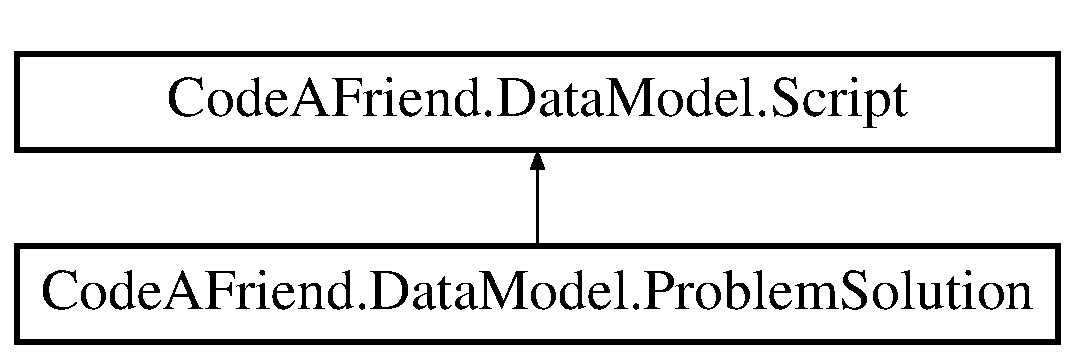
\includegraphics[height=2.000000cm]{class_code_a_friend_1_1_data_model_1_1_problem_solution}
\end{center}
\end{figure}
\subsection*{Public Member Functions}
\begin{DoxyCompactItemize}
\item 
\mbox{\hyperlink{class_code_a_friend_1_1_data_model_1_1_problem_solution_aa0d35cf0023de3ab3b42e433d607bccf}{Problem\+Solution}} (\mbox{\hyperlink{class_code_a_friend_1_1_data_model_1_1_user}{User}} submitter, \mbox{\hyperlink{class_code_a_friend_1_1_data_model_1_1_script}{Script}} script)
\begin{DoxyCompactList}\small\item\em Constructor for creating new \mbox{\hyperlink{class_code_a_friend_1_1_data_model_1_1_problem_solution}{Problem\+Solution}}.\end{DoxyCompactList}\item 
void \mbox{\hyperlink{class_code_a_friend_1_1_data_model_1_1_problem_solution_a2c0f0f4da13003471346d3d2101c4e04}{Add}} (\mbox{\hyperlink{class_code_a_friend_1_1_data_model_1_1_vote}{Vote}} vote, Db\+Context context=null)
\begin{DoxyCompactList}\small\item\em Add a \mbox{\hyperlink{class_code_a_friend_1_1_data_model_1_1_vote}{Vote}} to this \mbox{\hyperlink{class_code_a_friend_1_1_data_model_1_1_problem_solution}{Problem\+Solution}}. \end{DoxyCompactList}\end{DoxyCompactItemize}
\subsection*{Public Attributes}
\begin{DoxyCompactItemize}
\item 
I\+Enumerable$<$ \mbox{\hyperlink{class_code_a_friend_1_1_data_model_1_1_vote}{Vote}} $>$ \mbox{\hyperlink{class_code_a_friend_1_1_data_model_1_1_problem_solution_a6012ce280fdad237001766fb95a204ab}{Votes}} =$>$ \+\_\+votes?.To\+List()
\begin{DoxyCompactList}\small\item\em All votes submitted for this solution.\end{DoxyCompactList}\end{DoxyCompactItemize}
\subsection*{Protected Member Functions}
\begin{DoxyCompactItemize}
\item 
\mbox{\hyperlink{class_code_a_friend_1_1_data_model_1_1_problem_solution_aea496eef30d40476057177599c386555}{Problem\+Solution}} ()
\begin{DoxyCompactList}\small\item\em Parameterless Constructor required for EF.\end{DoxyCompactList}\end{DoxyCompactItemize}
\subsection*{Properties}
\begin{DoxyCompactItemize}
\item 
\mbox{\hyperlink{class_code_a_friend_1_1_data_model_1_1_user}{User}} \mbox{\hyperlink{class_code_a_friend_1_1_data_model_1_1_problem_solution_a3ca0acf918b42f59e4c8951b3e8cd68e}{Submitter}}\hspace{0.3cm}{\ttfamily  \mbox{[}get\mbox{]}}
\begin{DoxyCompactList}\small\item\em \mbox{\hyperlink{class_code_a_friend_1_1_data_model_1_1_user}{User}} who submitted this \mbox{\hyperlink{class_code_a_friend_1_1_data_model_1_1_problem_solution}{Problem\+Solution}}.\end{DoxyCompactList}\end{DoxyCompactItemize}


\subsection{Detailed Description}
A script that ran and successfully passed all test cases for a \mbox{\hyperlink{class_code_a_friend_1_1_data_model_1_1_problem}{Problem}}.



\subsection{Constructor \& Destructor Documentation}
\mbox{\Hypertarget{class_code_a_friend_1_1_data_model_1_1_problem_solution_aea496eef30d40476057177599c386555}\label{class_code_a_friend_1_1_data_model_1_1_problem_solution_aea496eef30d40476057177599c386555}} 
\index{Code\+A\+Friend\+::\+Data\+Model\+::\+Problem\+Solution@{Code\+A\+Friend\+::\+Data\+Model\+::\+Problem\+Solution}!Problem\+Solution@{Problem\+Solution}}
\index{Problem\+Solution@{Problem\+Solution}!Code\+A\+Friend\+::\+Data\+Model\+::\+Problem\+Solution@{Code\+A\+Friend\+::\+Data\+Model\+::\+Problem\+Solution}}
\subsubsection{\texorpdfstring{Problem\+Solution()}{ProblemSolution()}\hspace{0.1cm}{\footnotesize\ttfamily [1/2]}}
{\footnotesize\ttfamily Code\+A\+Friend.\+Data\+Model.\+Problem\+Solution.\+Problem\+Solution (\begin{DoxyParamCaption}{ }\end{DoxyParamCaption})\hspace{0.3cm}{\ttfamily [protected]}}



Parameterless Constructor required for EF.

\mbox{\Hypertarget{class_code_a_friend_1_1_data_model_1_1_problem_solution_aa0d35cf0023de3ab3b42e433d607bccf}\label{class_code_a_friend_1_1_data_model_1_1_problem_solution_aa0d35cf0023de3ab3b42e433d607bccf}} 
\index{Code\+A\+Friend\+::\+Data\+Model\+::\+Problem\+Solution@{Code\+A\+Friend\+::\+Data\+Model\+::\+Problem\+Solution}!Problem\+Solution@{Problem\+Solution}}
\index{Problem\+Solution@{Problem\+Solution}!Code\+A\+Friend\+::\+Data\+Model\+::\+Problem\+Solution@{Code\+A\+Friend\+::\+Data\+Model\+::\+Problem\+Solution}}
\subsubsection{\texorpdfstring{Problem\+Solution()}{ProblemSolution()}\hspace{0.1cm}{\footnotesize\ttfamily [2/2]}}
{\footnotesize\ttfamily Code\+A\+Friend.\+Data\+Model.\+Problem\+Solution.\+Problem\+Solution (\begin{DoxyParamCaption}\item[{\mbox{\hyperlink{class_code_a_friend_1_1_data_model_1_1_user}{User}}}]{submitter,  }\item[{\mbox{\hyperlink{class_code_a_friend_1_1_data_model_1_1_script}{Script}}}]{script }\end{DoxyParamCaption})}



Constructor for creating new \mbox{\hyperlink{class_code_a_friend_1_1_data_model_1_1_problem_solution}{Problem\+Solution}}.



\subsection{Member Function Documentation}
\mbox{\Hypertarget{class_code_a_friend_1_1_data_model_1_1_problem_solution_a2c0f0f4da13003471346d3d2101c4e04}\label{class_code_a_friend_1_1_data_model_1_1_problem_solution_a2c0f0f4da13003471346d3d2101c4e04}} 
\index{Code\+A\+Friend\+::\+Data\+Model\+::\+Problem\+Solution@{Code\+A\+Friend\+::\+Data\+Model\+::\+Problem\+Solution}!Add@{Add}}
\index{Add@{Add}!Code\+A\+Friend\+::\+Data\+Model\+::\+Problem\+Solution@{Code\+A\+Friend\+::\+Data\+Model\+::\+Problem\+Solution}}
\subsubsection{\texorpdfstring{Add()}{Add()}}
{\footnotesize\ttfamily void Code\+A\+Friend.\+Data\+Model.\+Problem\+Solution.\+Add (\begin{DoxyParamCaption}\item[{\mbox{\hyperlink{class_code_a_friend_1_1_data_model_1_1_vote}{Vote}}}]{vote,  }\item[{Db\+Context}]{context = {\ttfamily null} }\end{DoxyParamCaption})}



Add a \mbox{\hyperlink{class_code_a_friend_1_1_data_model_1_1_vote}{Vote}} to this \mbox{\hyperlink{class_code_a_friend_1_1_data_model_1_1_problem_solution}{Problem\+Solution}}. 


\begin{DoxyParams}{Parameters}
{\em vote} & \mbox{\hyperlink{class_code_a_friend_1_1_data_model_1_1_vote}{Vote}} to add.\\
\hline
{\em context} & Database to save the updated state to. (When Save\+Changes is called).\\
\hline
\end{DoxyParams}


\subsection{Member Data Documentation}
\mbox{\Hypertarget{class_code_a_friend_1_1_data_model_1_1_problem_solution_a6012ce280fdad237001766fb95a204ab}\label{class_code_a_friend_1_1_data_model_1_1_problem_solution_a6012ce280fdad237001766fb95a204ab}} 
\index{Code\+A\+Friend\+::\+Data\+Model\+::\+Problem\+Solution@{Code\+A\+Friend\+::\+Data\+Model\+::\+Problem\+Solution}!Votes@{Votes}}
\index{Votes@{Votes}!Code\+A\+Friend\+::\+Data\+Model\+::\+Problem\+Solution@{Code\+A\+Friend\+::\+Data\+Model\+::\+Problem\+Solution}}
\subsubsection{\texorpdfstring{Votes}{Votes}}
{\footnotesize\ttfamily I\+Enumerable$<$\mbox{\hyperlink{class_code_a_friend_1_1_data_model_1_1_vote}{Vote}}$>$ Code\+A\+Friend.\+Data\+Model.\+Problem\+Solution.\+Votes =$>$ \+\_\+votes?.To\+List()}



All votes submitted for this solution.



\subsection{Property Documentation}
\mbox{\Hypertarget{class_code_a_friend_1_1_data_model_1_1_problem_solution_a3ca0acf918b42f59e4c8951b3e8cd68e}\label{class_code_a_friend_1_1_data_model_1_1_problem_solution_a3ca0acf918b42f59e4c8951b3e8cd68e}} 
\index{Code\+A\+Friend\+::\+Data\+Model\+::\+Problem\+Solution@{Code\+A\+Friend\+::\+Data\+Model\+::\+Problem\+Solution}!Submitter@{Submitter}}
\index{Submitter@{Submitter}!Code\+A\+Friend\+::\+Data\+Model\+::\+Problem\+Solution@{Code\+A\+Friend\+::\+Data\+Model\+::\+Problem\+Solution}}
\subsubsection{\texorpdfstring{Submitter}{Submitter}}
{\footnotesize\ttfamily \mbox{\hyperlink{class_code_a_friend_1_1_data_model_1_1_user}{User}} Code\+A\+Friend.\+Data\+Model.\+Problem\+Solution.\+Submitter\hspace{0.3cm}{\ttfamily [get]}}



\mbox{\hyperlink{class_code_a_friend_1_1_data_model_1_1_user}{User}} who submitted this \mbox{\hyperlink{class_code_a_friend_1_1_data_model_1_1_problem_solution}{Problem\+Solution}}.



The documentation for this class was generated from the following file\+:\begin{DoxyCompactItemize}
\item 
shared/\+Code\+A\+Friend.\+Data\+Model/\+Problem\+Logic/\mbox{\hyperlink{_problem_solution_8cs}{Problem\+Solution.\+cs}}\end{DoxyCompactItemize}

\hypertarget{class_code_a_friend_1_1_api_service_1_1_program}{}\section{Code\+A\+Friend.\+Api\+Service.\+Program Class Reference}
\label{class_code_a_friend_1_1_api_service_1_1_program}\index{Code\+A\+Friend.\+Api\+Service.\+Program@{Code\+A\+Friend.\+Api\+Service.\+Program}}
\subsection*{Static Public Member Functions}
\begin{DoxyCompactItemize}
\item 
static void \mbox{\hyperlink{class_code_a_friend_1_1_api_service_1_1_program_ab8576d734dee8553d034caa706a0d54c}{Main}} (string\mbox{[}$\,$\mbox{]} args)
\item 
static I\+Web\+Host\+Builder \mbox{\hyperlink{class_code_a_friend_1_1_api_service_1_1_program_a14dd777c9ede20d6d0ef28d833963981}{Create\+Web\+Host\+Builder}} (string\mbox{[}$\,$\mbox{]} args)
\end{DoxyCompactItemize}


\subsection{Member Function Documentation}
\mbox{\Hypertarget{class_code_a_friend_1_1_api_service_1_1_program_a14dd777c9ede20d6d0ef28d833963981}\label{class_code_a_friend_1_1_api_service_1_1_program_a14dd777c9ede20d6d0ef28d833963981}} 
\index{Code\+A\+Friend\+::\+Api\+Service\+::\+Program@{Code\+A\+Friend\+::\+Api\+Service\+::\+Program}!Create\+Web\+Host\+Builder@{Create\+Web\+Host\+Builder}}
\index{Create\+Web\+Host\+Builder@{Create\+Web\+Host\+Builder}!Code\+A\+Friend\+::\+Api\+Service\+::\+Program@{Code\+A\+Friend\+::\+Api\+Service\+::\+Program}}
\subsubsection{\texorpdfstring{Create\+Web\+Host\+Builder()}{CreateWebHostBuilder()}}
{\footnotesize\ttfamily static I\+Web\+Host\+Builder Code\+A\+Friend.\+Api\+Service.\+Program.\+Create\+Web\+Host\+Builder (\begin{DoxyParamCaption}\item[{string \mbox{[}$\,$\mbox{]}}]{args }\end{DoxyParamCaption})\hspace{0.3cm}{\ttfamily [static]}}

\mbox{\Hypertarget{class_code_a_friend_1_1_api_service_1_1_program_ab8576d734dee8553d034caa706a0d54c}\label{class_code_a_friend_1_1_api_service_1_1_program_ab8576d734dee8553d034caa706a0d54c}} 
\index{Code\+A\+Friend\+::\+Api\+Service\+::\+Program@{Code\+A\+Friend\+::\+Api\+Service\+::\+Program}!Main@{Main}}
\index{Main@{Main}!Code\+A\+Friend\+::\+Api\+Service\+::\+Program@{Code\+A\+Friend\+::\+Api\+Service\+::\+Program}}
\subsubsection{\texorpdfstring{Main()}{Main()}}
{\footnotesize\ttfamily static void Code\+A\+Friend.\+Api\+Service.\+Program.\+Main (\begin{DoxyParamCaption}\item[{string \mbox{[}$\,$\mbox{]}}]{args }\end{DoxyParamCaption})\hspace{0.3cm}{\ttfamily [static]}}



The documentation for this class was generated from the following file\+:\begin{DoxyCompactItemize}
\item 
apps/\+Code\+A\+Friend.\+Api\+Service/\mbox{\hyperlink{_program_8cs}{Program.\+cs}}\end{DoxyCompactItemize}

\hypertarget{class_code_a_friend_1_1_languages_1_1_python2_1_1_python27_interpreter}{}\section{Code\+A\+Friend.\+Languages.\+Python2.\+Python27\+Interpreter Class Reference}
\label{class_code_a_friend_1_1_languages_1_1_python2_1_1_python27_interpreter}\index{Code\+A\+Friend.\+Languages.\+Python2.\+Python27\+Interpreter@{Code\+A\+Friend.\+Languages.\+Python2.\+Python27\+Interpreter}}


 


Inheritance diagram for Code\+A\+Friend.\+Languages.\+Python2.\+Python27\+Interpreter\+:\begin{figure}[H]
\begin{center}
\leavevmode
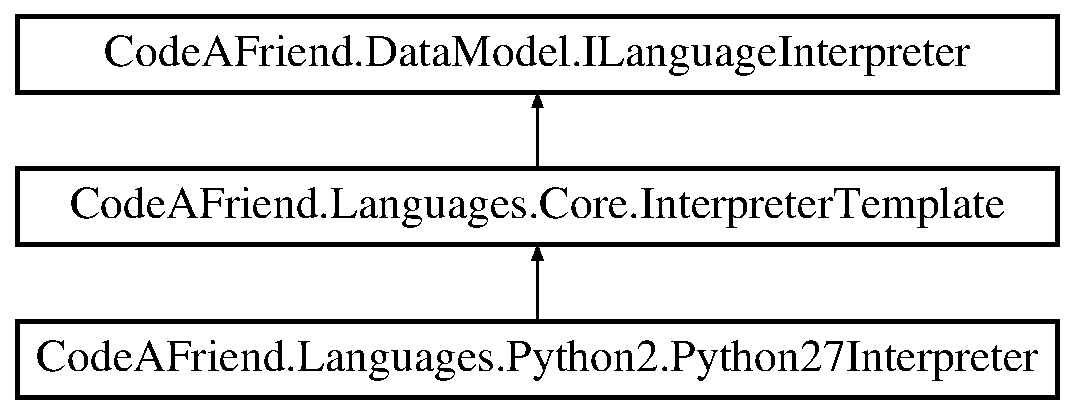
\includegraphics[height=3.000000cm]{class_code_a_friend_1_1_languages_1_1_python2_1_1_python27_interpreter}
\end{center}
\end{figure}
\subsection*{Public Member Functions}
\begin{DoxyCompactItemize}
\item 
override Process\+Start\+Info \mbox{\hyperlink{class_code_a_friend_1_1_languages_1_1_python2_1_1_python27_interpreter_a24b4f1f296ab282b0fcac3951af0a73b}{Get\+Process\+Start\+Info}} (string script\+File\+Path)
\end{DoxyCompactItemize}
\subsection*{Static Public Member Functions}
\begin{DoxyCompactItemize}
\item 
static async Task \mbox{\hyperlink{class_code_a_friend_1_1_languages_1_1_python2_1_1_python27_interpreter_a81b2649dd7c6a7dc934efbd27e14377b}{Main}} (string\mbox{[}$\,$\mbox{]} args)
\item 
static async Task$<$ string $>$ \mbox{\hyperlink{class_code_a_friend_1_1_languages_1_1_python2_1_1_python27_interpreter_ad72980fe0c53ba1da906f2e5c5b04c19}{Run\+Engine\+Async}} (string script\+Body)
\end{DoxyCompactItemize}
\subsection*{Properties}
\begin{DoxyCompactItemize}
\item 
override \mbox{\hyperlink{namespace_code_a_friend_1_1_data_model_a13e088c525db1b03a4de75420ced79b2}{Supported\+Language}} \mbox{\hyperlink{class_code_a_friend_1_1_languages_1_1_python2_1_1_python27_interpreter_aeae6049e330cf5a2d73e11b242b62b62}{Name}} = Supported\+Language.\+Python27\hspace{0.3cm}{\ttfamily  \mbox{[}get\mbox{]}}
\end{DoxyCompactItemize}


\subsection{Detailed Description}




\subsection{Member Function Documentation}
\mbox{\Hypertarget{class_code_a_friend_1_1_languages_1_1_python2_1_1_python27_interpreter_a24b4f1f296ab282b0fcac3951af0a73b}\label{class_code_a_friend_1_1_languages_1_1_python2_1_1_python27_interpreter_a24b4f1f296ab282b0fcac3951af0a73b}} 
\index{Code\+A\+Friend\+::\+Languages\+::\+Python2\+::\+Python27\+Interpreter@{Code\+A\+Friend\+::\+Languages\+::\+Python2\+::\+Python27\+Interpreter}!Get\+Process\+Start\+Info@{Get\+Process\+Start\+Info}}
\index{Get\+Process\+Start\+Info@{Get\+Process\+Start\+Info}!Code\+A\+Friend\+::\+Languages\+::\+Python2\+::\+Python27\+Interpreter@{Code\+A\+Friend\+::\+Languages\+::\+Python2\+::\+Python27\+Interpreter}}
\subsubsection{\texorpdfstring{Get\+Process\+Start\+Info()}{GetProcessStartInfo()}}
{\footnotesize\ttfamily override Process\+Start\+Info Code\+A\+Friend.\+Languages.\+Python2.\+Python27\+Interpreter.\+Get\+Process\+Start\+Info (\begin{DoxyParamCaption}\item[{string}]{script\+File\+Path }\end{DoxyParamCaption})\hspace{0.3cm}{\ttfamily [virtual]}}

from \href{https://medium.com/emoney-engineering/running-python-script-from-c-and-working-with-the-results-843e68d230e5}{\tt https\+://medium.\+com/emoney-\/engineering/running-\/python-\/script-\/from-\/c-\/and-\/working-\/with-\/the-\/results-\/843e68d230e5} . \href{https://kimsereyblog.blogspot.com/2018/01/start-processes-from-c-in-dotnet-core.html}{\tt https\+://kimsereyblog.\+blogspot.\+com/2018/01/start-\/processes-\/from-\/c-\/in-\/dotnet-\/core.\+html} 

Implements \mbox{\hyperlink{class_code_a_friend_1_1_languages_1_1_core_1_1_interpreter_template_a2f8560fba2e22a9cdf22c8d2f7bb849f}{Code\+A\+Friend.\+Languages.\+Core.\+Interpreter\+Template}}.

\mbox{\Hypertarget{class_code_a_friend_1_1_languages_1_1_python2_1_1_python27_interpreter_a81b2649dd7c6a7dc934efbd27e14377b}\label{class_code_a_friend_1_1_languages_1_1_python2_1_1_python27_interpreter_a81b2649dd7c6a7dc934efbd27e14377b}} 
\index{Code\+A\+Friend\+::\+Languages\+::\+Python2\+::\+Python27\+Interpreter@{Code\+A\+Friend\+::\+Languages\+::\+Python2\+::\+Python27\+Interpreter}!Main@{Main}}
\index{Main@{Main}!Code\+A\+Friend\+::\+Languages\+::\+Python2\+::\+Python27\+Interpreter@{Code\+A\+Friend\+::\+Languages\+::\+Python2\+::\+Python27\+Interpreter}}
\subsubsection{\texorpdfstring{Main()}{Main()}}
{\footnotesize\ttfamily static async Task Code\+A\+Friend.\+Languages.\+Python2.\+Python27\+Interpreter.\+Main (\begin{DoxyParamCaption}\item[{string \mbox{[}$\,$\mbox{]}}]{args }\end{DoxyParamCaption})\hspace{0.3cm}{\ttfamily [static]}}

\mbox{\Hypertarget{class_code_a_friend_1_1_languages_1_1_python2_1_1_python27_interpreter_ad72980fe0c53ba1da906f2e5c5b04c19}\label{class_code_a_friend_1_1_languages_1_1_python2_1_1_python27_interpreter_ad72980fe0c53ba1da906f2e5c5b04c19}} 
\index{Code\+A\+Friend\+::\+Languages\+::\+Python2\+::\+Python27\+Interpreter@{Code\+A\+Friend\+::\+Languages\+::\+Python2\+::\+Python27\+Interpreter}!Run\+Engine\+Async@{Run\+Engine\+Async}}
\index{Run\+Engine\+Async@{Run\+Engine\+Async}!Code\+A\+Friend\+::\+Languages\+::\+Python2\+::\+Python27\+Interpreter@{Code\+A\+Friend\+::\+Languages\+::\+Python2\+::\+Python27\+Interpreter}}
\subsubsection{\texorpdfstring{Run\+Engine\+Async()}{RunEngineAsync()}}
{\footnotesize\ttfamily static async Task$<$string$>$ Code\+A\+Friend.\+Languages.\+Python2.\+Python27\+Interpreter.\+Run\+Engine\+Async (\begin{DoxyParamCaption}\item[{string}]{script\+Body }\end{DoxyParamCaption})\hspace{0.3cm}{\ttfamily [static]}}

from \href{https://medium.com/emoney-engineering/running-python-script-from-c-and-working-with-the-results-843e68d230e5}{\tt https\+://medium.\+com/emoney-\/engineering/running-\/python-\/script-\/from-\/c-\/and-\/working-\/with-\/the-\/results-\/843e68d230e5} 

\subsection{Property Documentation}
\mbox{\Hypertarget{class_code_a_friend_1_1_languages_1_1_python2_1_1_python27_interpreter_aeae6049e330cf5a2d73e11b242b62b62}\label{class_code_a_friend_1_1_languages_1_1_python2_1_1_python27_interpreter_aeae6049e330cf5a2d73e11b242b62b62}} 
\index{Code\+A\+Friend\+::\+Languages\+::\+Python2\+::\+Python27\+Interpreter@{Code\+A\+Friend\+::\+Languages\+::\+Python2\+::\+Python27\+Interpreter}!Name@{Name}}
\index{Name@{Name}!Code\+A\+Friend\+::\+Languages\+::\+Python2\+::\+Python27\+Interpreter@{Code\+A\+Friend\+::\+Languages\+::\+Python2\+::\+Python27\+Interpreter}}
\subsubsection{\texorpdfstring{Name}{Name}}
{\footnotesize\ttfamily override \mbox{\hyperlink{namespace_code_a_friend_1_1_data_model_a13e088c525db1b03a4de75420ced79b2}{Supported\+Language}} Code\+A\+Friend.\+Languages.\+Python2.\+Python27\+Interpreter.\+Name = Supported\+Language.\+Python27\hspace{0.3cm}{\ttfamily [get]}}







The documentation for this class was generated from the following file\+:\begin{DoxyCompactItemize}
\item 
shared/\+Code\+A\+Friend.\+Languages.\+Python2/\mbox{\hyperlink{_python27_interpreter_8cs}{Python27\+Interpreter.\+cs}}\end{DoxyCompactItemize}

\hypertarget{class_code_a_friend_1_1_languages_1_1_python3_1_1_python37_interpreter}{}\section{Code\+A\+Friend.\+Languages.\+Python3.\+Python37\+Interpreter Class Reference}
\label{class_code_a_friend_1_1_languages_1_1_python3_1_1_python37_interpreter}\index{Code\+A\+Friend.\+Languages.\+Python3.\+Python37\+Interpreter@{Code\+A\+Friend.\+Languages.\+Python3.\+Python37\+Interpreter}}


Implementation of I\+Language\+Interpreter for Python programming language.  


Inheritance diagram for Code\+A\+Friend.\+Languages.\+Python3.\+Python37\+Interpreter\+:\begin{figure}[H]
\begin{center}
\leavevmode
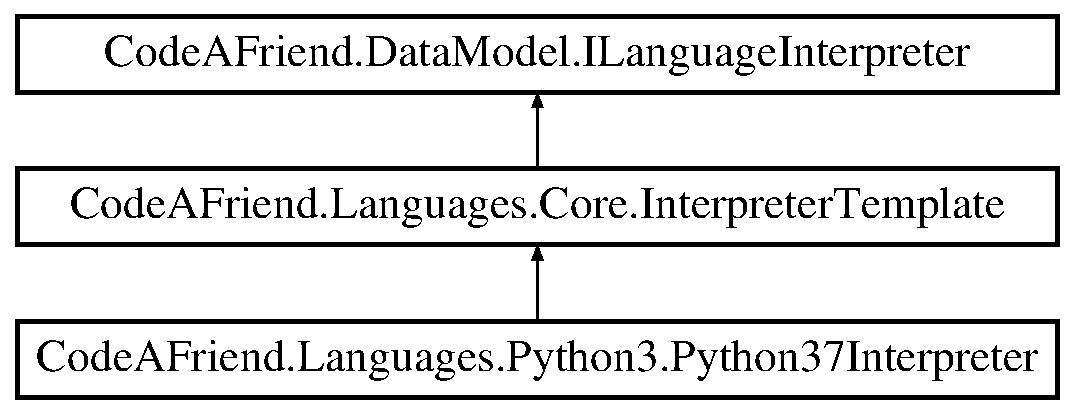
\includegraphics[height=3.000000cm]{class_code_a_friend_1_1_languages_1_1_python3_1_1_python37_interpreter}
\end{center}
\end{figure}
\subsection*{Public Member Functions}
\begin{DoxyCompactItemize}
\item 
override Process\+Start\+Info \mbox{\hyperlink{class_code_a_friend_1_1_languages_1_1_python3_1_1_python37_interpreter_a61f777c41849f97cd94eccee5fe7c617}{Get\+Process\+Start\+Info}} (string script\+File\+Path)
\end{DoxyCompactItemize}
\subsection*{Properties}
\begin{DoxyCompactItemize}
\item 
override \mbox{\hyperlink{namespace_code_a_friend_1_1_data_model_a13e088c525db1b03a4de75420ced79b2}{Supported\+Language}} \mbox{\hyperlink{class_code_a_friend_1_1_languages_1_1_python3_1_1_python37_interpreter_a8cb30396a002b58c37ead323fae59383}{Name}} = Supported\+Language.\+Python37\hspace{0.3cm}{\ttfamily  \mbox{[}get\mbox{]}}
\end{DoxyCompactItemize}


\subsection{Detailed Description}
Implementation of I\+Language\+Interpreter for Python programming language. 



\subsection{Member Function Documentation}
\mbox{\Hypertarget{class_code_a_friend_1_1_languages_1_1_python3_1_1_python37_interpreter_a61f777c41849f97cd94eccee5fe7c617}\label{class_code_a_friend_1_1_languages_1_1_python3_1_1_python37_interpreter_a61f777c41849f97cd94eccee5fe7c617}} 
\index{Code\+A\+Friend\+::\+Languages\+::\+Python3\+::\+Python37\+Interpreter@{Code\+A\+Friend\+::\+Languages\+::\+Python3\+::\+Python37\+Interpreter}!Get\+Process\+Start\+Info@{Get\+Process\+Start\+Info}}
\index{Get\+Process\+Start\+Info@{Get\+Process\+Start\+Info}!Code\+A\+Friend\+::\+Languages\+::\+Python3\+::\+Python37\+Interpreter@{Code\+A\+Friend\+::\+Languages\+::\+Python3\+::\+Python37\+Interpreter}}
\subsubsection{\texorpdfstring{Get\+Process\+Start\+Info()}{GetProcessStartInfo()}}
{\footnotesize\ttfamily override Process\+Start\+Info Code\+A\+Friend.\+Languages.\+Python3.\+Python37\+Interpreter.\+Get\+Process\+Start\+Info (\begin{DoxyParamCaption}\item[{string}]{script\+File\+Path }\end{DoxyParamCaption})\hspace{0.3cm}{\ttfamily [virtual]}}

run to create an alias ~\newline
doskey python3=\char`\"{}\+C\+:\textbackslash{}\+Program Files\textbackslash{}\+Python37\textbackslash{}python.\+exe\char`\"{} 

Implements \mbox{\hyperlink{class_code_a_friend_1_1_languages_1_1_core_1_1_interpreter_template_a2f8560fba2e22a9cdf22c8d2f7bb849f}{Code\+A\+Friend.\+Languages.\+Core.\+Interpreter\+Template}}.



\subsection{Property Documentation}
\mbox{\Hypertarget{class_code_a_friend_1_1_languages_1_1_python3_1_1_python37_interpreter_a8cb30396a002b58c37ead323fae59383}\label{class_code_a_friend_1_1_languages_1_1_python3_1_1_python37_interpreter_a8cb30396a002b58c37ead323fae59383}} 
\index{Code\+A\+Friend\+::\+Languages\+::\+Python3\+::\+Python37\+Interpreter@{Code\+A\+Friend\+::\+Languages\+::\+Python3\+::\+Python37\+Interpreter}!Name@{Name}}
\index{Name@{Name}!Code\+A\+Friend\+::\+Languages\+::\+Python3\+::\+Python37\+Interpreter@{Code\+A\+Friend\+::\+Languages\+::\+Python3\+::\+Python37\+Interpreter}}
\subsubsection{\texorpdfstring{Name}{Name}}
{\footnotesize\ttfamily override \mbox{\hyperlink{namespace_code_a_friend_1_1_data_model_a13e088c525db1b03a4de75420ced79b2}{Supported\+Language}} Code\+A\+Friend.\+Languages.\+Python3.\+Python37\+Interpreter.\+Name = Supported\+Language.\+Python37\hspace{0.3cm}{\ttfamily [get]}}







The documentation for this class was generated from the following file\+:\begin{DoxyCompactItemize}
\item 
shared/\+Code\+A\+Friend.\+Languages.\+Python3/\mbox{\hyperlink{_python37_interpreter_8cs}{Python37\+Interpreter.\+cs}}\end{DoxyCompactItemize}

\hypertarget{class_code_a_friend_1_1_data_model_1_1_script}{}\section{Code\+A\+Friend.\+Data\+Model.\+Script Class Reference}
\label{class_code_a_friend_1_1_data_model_1_1_script}\index{Code\+A\+Friend.\+Data\+Model.\+Script@{Code\+A\+Friend.\+Data\+Model.\+Script}}


A piece of code to be compiled in a specified language.  


Inheritance diagram for Code\+A\+Friend.\+Data\+Model.\+Script\+:\begin{figure}[H]
\begin{center}
\leavevmode
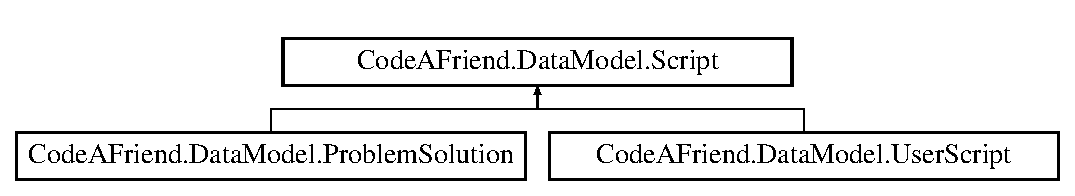
\includegraphics[height=2.000000cm]{class_code_a_friend_1_1_data_model_1_1_script}
\end{center}
\end{figure}
\subsection*{Public Member Functions}
\begin{DoxyCompactItemize}
\item 
\mbox{\hyperlink{class_code_a_friend_1_1_data_model_1_1_script_a1f92caf940d4376a3f2e96833b3ee029}{Script}} (string name, string body, \mbox{\hyperlink{namespace_code_a_friend_1_1_data_model_a13e088c525db1b03a4de75420ced79b2}{Supported\+Language}} language)
\begin{DoxyCompactList}\small\item\em Constructor for creating new \mbox{\hyperlink{class_code_a_friend_1_1_data_model_1_1_script}{Script}}.\end{DoxyCompactList}\item 
\mbox{\hyperlink{class_code_a_friend_1_1_data_model_1_1_script}{Script}} \mbox{\hyperlink{class_code_a_friend_1_1_data_model_1_1_script_a02124202d7f885992a243853531b3216}{Clone}} ()
\begin{DoxyCompactList}\small\item\em Create a deep copy of this \mbox{\hyperlink{class_code_a_friend_1_1_data_model_1_1_script}{Script}}. \end{DoxyCompactList}\end{DoxyCompactItemize}
\subsection*{Properties}
\begin{DoxyCompactItemize}
\item 
Guid \mbox{\hyperlink{class_code_a_friend_1_1_data_model_1_1_script_a91e1a0a804f19d83f904871d33998ce7}{Id}}\hspace{0.3cm}{\ttfamily  \mbox{[}get\mbox{]}}
\begin{DoxyCompactList}\small\item\em Unique Id assigned to the \mbox{\hyperlink{class_code_a_friend_1_1_data_model_1_1_script}{Script}} during creation.\end{DoxyCompactList}\item 
string \mbox{\hyperlink{class_code_a_friend_1_1_data_model_1_1_script_aa075f49454db91a785b8147c2b85bb54}{Name}}\hspace{0.3cm}{\ttfamily  \mbox{[}get\mbox{]}}
\begin{DoxyCompactList}\small\item\em Name given to this script by the user who created it.\end{DoxyCompactList}\item 
string \mbox{\hyperlink{class_code_a_friend_1_1_data_model_1_1_script_a8d73e309856111b7666fe48f1b613eda}{Body}}\hspace{0.3cm}{\ttfamily  \mbox{[}get\mbox{]}}
\begin{DoxyCompactList}\small\item\em Code.\end{DoxyCompactList}\item 
\mbox{\hyperlink{namespace_code_a_friend_1_1_data_model_a13e088c525db1b03a4de75420ced79b2}{Supported\+Language}} \mbox{\hyperlink{class_code_a_friend_1_1_data_model_1_1_script_a02cc66f28767d1548f3b153d4c2e1840}{Language}}\hspace{0.3cm}{\ttfamily  \mbox{[}get\mbox{]}}
\begin{DoxyCompactList}\small\item\em Language to compile code in.\end{DoxyCompactList}\end{DoxyCompactItemize}


\subsection{Detailed Description}
A piece of code to be compiled in a specified language. 



\subsection{Constructor \& Destructor Documentation}
\mbox{\Hypertarget{class_code_a_friend_1_1_data_model_1_1_script_a1f92caf940d4376a3f2e96833b3ee029}\label{class_code_a_friend_1_1_data_model_1_1_script_a1f92caf940d4376a3f2e96833b3ee029}} 
\index{Code\+A\+Friend\+::\+Data\+Model\+::\+Script@{Code\+A\+Friend\+::\+Data\+Model\+::\+Script}!Script@{Script}}
\index{Script@{Script}!Code\+A\+Friend\+::\+Data\+Model\+::\+Script@{Code\+A\+Friend\+::\+Data\+Model\+::\+Script}}
\subsubsection{\texorpdfstring{Script()}{Script()}}
{\footnotesize\ttfamily Code\+A\+Friend.\+Data\+Model.\+Script.\+Script (\begin{DoxyParamCaption}\item[{string}]{name,  }\item[{string}]{body,  }\item[{\mbox{\hyperlink{namespace_code_a_friend_1_1_data_model_a13e088c525db1b03a4de75420ced79b2}{Supported\+Language}}}]{language }\end{DoxyParamCaption})}



Constructor for creating new \mbox{\hyperlink{class_code_a_friend_1_1_data_model_1_1_script}{Script}}.



\subsection{Member Function Documentation}
\mbox{\Hypertarget{class_code_a_friend_1_1_data_model_1_1_script_a02124202d7f885992a243853531b3216}\label{class_code_a_friend_1_1_data_model_1_1_script_a02124202d7f885992a243853531b3216}} 
\index{Code\+A\+Friend\+::\+Data\+Model\+::\+Script@{Code\+A\+Friend\+::\+Data\+Model\+::\+Script}!Clone@{Clone}}
\index{Clone@{Clone}!Code\+A\+Friend\+::\+Data\+Model\+::\+Script@{Code\+A\+Friend\+::\+Data\+Model\+::\+Script}}
\subsubsection{\texorpdfstring{Clone()}{Clone()}}
{\footnotesize\ttfamily \mbox{\hyperlink{class_code_a_friend_1_1_data_model_1_1_script}{Script}} Code\+A\+Friend.\+Data\+Model.\+Script.\+Clone (\begin{DoxyParamCaption}{ }\end{DoxyParamCaption})}



Create a deep copy of this \mbox{\hyperlink{class_code_a_friend_1_1_data_model_1_1_script}{Script}}. 

Employs the Prototype design pattern.

\begin{DoxyReturn}{Returns}
\mbox{\hyperlink{class_code_a_friend_1_1_data_model_1_1_script}{Script}} object that is a deep copy of this \mbox{\hyperlink{class_code_a_friend_1_1_data_model_1_1_script}{Script}}.
\end{DoxyReturn}


\subsection{Property Documentation}
\mbox{\Hypertarget{class_code_a_friend_1_1_data_model_1_1_script_a8d73e309856111b7666fe48f1b613eda}\label{class_code_a_friend_1_1_data_model_1_1_script_a8d73e309856111b7666fe48f1b613eda}} 
\index{Code\+A\+Friend\+::\+Data\+Model\+::\+Script@{Code\+A\+Friend\+::\+Data\+Model\+::\+Script}!Body@{Body}}
\index{Body@{Body}!Code\+A\+Friend\+::\+Data\+Model\+::\+Script@{Code\+A\+Friend\+::\+Data\+Model\+::\+Script}}
\subsubsection{\texorpdfstring{Body}{Body}}
{\footnotesize\ttfamily string Code\+A\+Friend.\+Data\+Model.\+Script.\+Body\hspace{0.3cm}{\ttfamily [get]}}



Code.

\mbox{\Hypertarget{class_code_a_friend_1_1_data_model_1_1_script_a91e1a0a804f19d83f904871d33998ce7}\label{class_code_a_friend_1_1_data_model_1_1_script_a91e1a0a804f19d83f904871d33998ce7}} 
\index{Code\+A\+Friend\+::\+Data\+Model\+::\+Script@{Code\+A\+Friend\+::\+Data\+Model\+::\+Script}!Id@{Id}}
\index{Id@{Id}!Code\+A\+Friend\+::\+Data\+Model\+::\+Script@{Code\+A\+Friend\+::\+Data\+Model\+::\+Script}}
\subsubsection{\texorpdfstring{Id}{Id}}
{\footnotesize\ttfamily Guid Code\+A\+Friend.\+Data\+Model.\+Script.\+Id\hspace{0.3cm}{\ttfamily [get]}}



Unique Id assigned to the \mbox{\hyperlink{class_code_a_friend_1_1_data_model_1_1_script}{Script}} during creation.

\mbox{\Hypertarget{class_code_a_friend_1_1_data_model_1_1_script_a02cc66f28767d1548f3b153d4c2e1840}\label{class_code_a_friend_1_1_data_model_1_1_script_a02cc66f28767d1548f3b153d4c2e1840}} 
\index{Code\+A\+Friend\+::\+Data\+Model\+::\+Script@{Code\+A\+Friend\+::\+Data\+Model\+::\+Script}!Language@{Language}}
\index{Language@{Language}!Code\+A\+Friend\+::\+Data\+Model\+::\+Script@{Code\+A\+Friend\+::\+Data\+Model\+::\+Script}}
\subsubsection{\texorpdfstring{Language}{Language}}
{\footnotesize\ttfamily \mbox{\hyperlink{namespace_code_a_friend_1_1_data_model_a13e088c525db1b03a4de75420ced79b2}{Supported\+Language}} Code\+A\+Friend.\+Data\+Model.\+Script.\+Language\hspace{0.3cm}{\ttfamily [get]}}



Language to compile code in.

\mbox{\Hypertarget{class_code_a_friend_1_1_data_model_1_1_script_aa075f49454db91a785b8147c2b85bb54}\label{class_code_a_friend_1_1_data_model_1_1_script_aa075f49454db91a785b8147c2b85bb54}} 
\index{Code\+A\+Friend\+::\+Data\+Model\+::\+Script@{Code\+A\+Friend\+::\+Data\+Model\+::\+Script}!Name@{Name}}
\index{Name@{Name}!Code\+A\+Friend\+::\+Data\+Model\+::\+Script@{Code\+A\+Friend\+::\+Data\+Model\+::\+Script}}
\subsubsection{\texorpdfstring{Name}{Name}}
{\footnotesize\ttfamily string Code\+A\+Friend.\+Data\+Model.\+Script.\+Name\hspace{0.3cm}{\ttfamily [get]}}



Name given to this script by the user who created it.



The documentation for this class was generated from the following file\+:\begin{DoxyCompactItemize}
\item 
shared/\+Code\+A\+Friend.\+Data\+Model/\+Script\+Logic/\mbox{\hyperlink{_script_8cs}{Script.\+cs}}\end{DoxyCompactItemize}

\hypertarget{class_code_a_friend_1_1_data_model_1_1_script_evaluation}{}\section{Code\+A\+Friend.\+Data\+Model.\+Script\+Evaluation Class Reference}
\label{class_code_a_friend_1_1_data_model_1_1_script_evaluation}\index{Code\+A\+Friend.\+Data\+Model.\+Script\+Evaluation@{Code\+A\+Friend.\+Data\+Model.\+Script\+Evaluation}}


Results from executing a \mbox{\hyperlink{class_code_a_friend_1_1_data_model_1_1_script}{Script}} using specified \mbox{\hyperlink{class_code_a_friend_1_1_data_model_1_1_execution_parameters}{Execution\+Parameters}}.  


\subsection*{Public Member Functions}
\begin{DoxyCompactItemize}
\item 
\mbox{\hyperlink{class_code_a_friend_1_1_data_model_1_1_script_evaluation_abd3a2ec93bde80977a8c2b6609178a88}{Script\+Evaluation}} (string output, double cpu\+Time, long memory\+Usage)
\begin{DoxyCompactList}\small\item\em All Properties constructor. \end{DoxyCompactList}\end{DoxyCompactItemize}
\subsection*{Properties}
\begin{DoxyCompactItemize}
\item 
string \mbox{\hyperlink{class_code_a_friend_1_1_data_model_1_1_script_evaluation_ad90120cfe537b3a21bfc497d544eb0e9}{Output}}\hspace{0.3cm}{\ttfamily  \mbox{[}get, set\mbox{]}}
\begin{DoxyCompactList}\small\item\em Characters printed to stdout by the program during execution. \end{DoxyCompactList}\item 
double \mbox{\hyperlink{class_code_a_friend_1_1_data_model_1_1_script_evaluation_af4aa3fb175cd5fc2d6998c4690f5085e}{Cpu\+Time}}\hspace{0.3cm}{\ttfamily  \mbox{[}get, set\mbox{]}}
\begin{DoxyCompactList}\small\item\em Amount of time that the program took to complete execution. \end{DoxyCompactList}\item 
long \mbox{\hyperlink{class_code_a_friend_1_1_data_model_1_1_script_evaluation_a7a256f081758e46dabfbf3fae1c71817}{Memory\+Usage}}\hspace{0.3cm}{\ttfamily  \mbox{[}get, set\mbox{]}}
\begin{DoxyCompactList}\small\item\em Peak memory usage, by the program, during execution. \end{DoxyCompactList}\end{DoxyCompactItemize}


\subsection{Detailed Description}
Results from executing a \mbox{\hyperlink{class_code_a_friend_1_1_data_model_1_1_script}{Script}} using specified \mbox{\hyperlink{class_code_a_friend_1_1_data_model_1_1_execution_parameters}{Execution\+Parameters}}. 



\subsection{Constructor \& Destructor Documentation}
\mbox{\Hypertarget{class_code_a_friend_1_1_data_model_1_1_script_evaluation_abd3a2ec93bde80977a8c2b6609178a88}\label{class_code_a_friend_1_1_data_model_1_1_script_evaluation_abd3a2ec93bde80977a8c2b6609178a88}} 
\index{Code\+A\+Friend\+::\+Data\+Model\+::\+Script\+Evaluation@{Code\+A\+Friend\+::\+Data\+Model\+::\+Script\+Evaluation}!Script\+Evaluation@{Script\+Evaluation}}
\index{Script\+Evaluation@{Script\+Evaluation}!Code\+A\+Friend\+::\+Data\+Model\+::\+Script\+Evaluation@{Code\+A\+Friend\+::\+Data\+Model\+::\+Script\+Evaluation}}
\subsubsection{\texorpdfstring{Script\+Evaluation()}{ScriptEvaluation()}}
{\footnotesize\ttfamily Code\+A\+Friend.\+Data\+Model.\+Script\+Evaluation.\+Script\+Evaluation (\begin{DoxyParamCaption}\item[{string}]{output,  }\item[{double}]{cpu\+Time,  }\item[{long}]{memory\+Usage }\end{DoxyParamCaption})}



All Properties constructor. 



\subsection{Property Documentation}
\mbox{\Hypertarget{class_code_a_friend_1_1_data_model_1_1_script_evaluation_af4aa3fb175cd5fc2d6998c4690f5085e}\label{class_code_a_friend_1_1_data_model_1_1_script_evaluation_af4aa3fb175cd5fc2d6998c4690f5085e}} 
\index{Code\+A\+Friend\+::\+Data\+Model\+::\+Script\+Evaluation@{Code\+A\+Friend\+::\+Data\+Model\+::\+Script\+Evaluation}!Cpu\+Time@{Cpu\+Time}}
\index{Cpu\+Time@{Cpu\+Time}!Code\+A\+Friend\+::\+Data\+Model\+::\+Script\+Evaluation@{Code\+A\+Friend\+::\+Data\+Model\+::\+Script\+Evaluation}}
\subsubsection{\texorpdfstring{Cpu\+Time}{CpuTime}}
{\footnotesize\ttfamily double Code\+A\+Friend.\+Data\+Model.\+Script\+Evaluation.\+Cpu\+Time\hspace{0.3cm}{\ttfamily [get]}, {\ttfamily [set]}}



Amount of time that the program took to complete execution. 

\mbox{\Hypertarget{class_code_a_friend_1_1_data_model_1_1_script_evaluation_a7a256f081758e46dabfbf3fae1c71817}\label{class_code_a_friend_1_1_data_model_1_1_script_evaluation_a7a256f081758e46dabfbf3fae1c71817}} 
\index{Code\+A\+Friend\+::\+Data\+Model\+::\+Script\+Evaluation@{Code\+A\+Friend\+::\+Data\+Model\+::\+Script\+Evaluation}!Memory\+Usage@{Memory\+Usage}}
\index{Memory\+Usage@{Memory\+Usage}!Code\+A\+Friend\+::\+Data\+Model\+::\+Script\+Evaluation@{Code\+A\+Friend\+::\+Data\+Model\+::\+Script\+Evaluation}}
\subsubsection{\texorpdfstring{Memory\+Usage}{MemoryUsage}}
{\footnotesize\ttfamily long Code\+A\+Friend.\+Data\+Model.\+Script\+Evaluation.\+Memory\+Usage\hspace{0.3cm}{\ttfamily [get]}, {\ttfamily [set]}}



Peak memory usage, by the program, during execution. 

\mbox{\Hypertarget{class_code_a_friend_1_1_data_model_1_1_script_evaluation_ad90120cfe537b3a21bfc497d544eb0e9}\label{class_code_a_friend_1_1_data_model_1_1_script_evaluation_ad90120cfe537b3a21bfc497d544eb0e9}} 
\index{Code\+A\+Friend\+::\+Data\+Model\+::\+Script\+Evaluation@{Code\+A\+Friend\+::\+Data\+Model\+::\+Script\+Evaluation}!Output@{Output}}
\index{Output@{Output}!Code\+A\+Friend\+::\+Data\+Model\+::\+Script\+Evaluation@{Code\+A\+Friend\+::\+Data\+Model\+::\+Script\+Evaluation}}
\subsubsection{\texorpdfstring{Output}{Output}}
{\footnotesize\ttfamily string Code\+A\+Friend.\+Data\+Model.\+Script\+Evaluation.\+Output\hspace{0.3cm}{\ttfamily [get]}, {\ttfamily [set]}}



Characters printed to stdout by the program during execution. 



The documentation for this class was generated from the following file\+:\begin{DoxyCompactItemize}
\item 
shared/\+Code\+A\+Friend.\+Data\+Model/\+Script\+Logic/\mbox{\hyperlink{_script_evaluation_8cs}{Script\+Evaluation.\+cs}}\end{DoxyCompactItemize}

\hypertarget{class_code_a_friend_1_1_api_service_1_1_controllers_1_1_scripts_controller}{}\section{Code\+A\+Friend.\+Api\+Service.\+Controllers.\+Scripts\+Controller Class Reference}
\label{class_code_a_friend_1_1_api_service_1_1_controllers_1_1_scripts_controller}\index{Code\+A\+Friend.\+Api\+Service.\+Controllers.\+Scripts\+Controller@{Code\+A\+Friend.\+Api\+Service.\+Controllers.\+Scripts\+Controller}}


 


Inheritance diagram for Code\+A\+Friend.\+Api\+Service.\+Controllers.\+Scripts\+Controller\+:\begin{figure}[H]
\begin{center}
\leavevmode
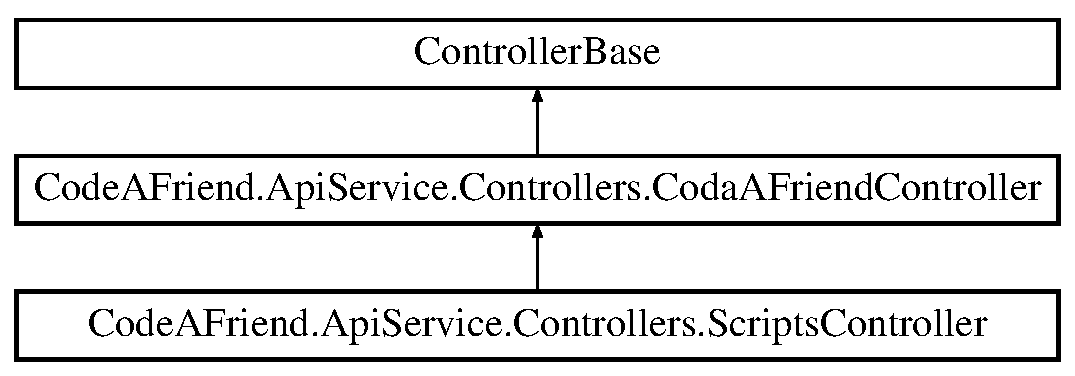
\includegraphics[height=3.000000cm]{class_code_a_friend_1_1_api_service_1_1_controllers_1_1_scripts_controller}
\end{center}
\end{figure}
\subsection*{Public Member Functions}
\begin{DoxyCompactItemize}
\item 
async Task$<$ I\+Action\+Result $>$ \mbox{\hyperlink{class_code_a_friend_1_1_api_service_1_1_controllers_1_1_scripts_controller_a65b4e550a6af06c510d0b4427c7fb7c6}{Add\+User\+Script}} (\mbox{\hyperlink{class_code_a_friend_1_1_data_model_1_1_user_1_1_add_script_command}{User.\+Add\+Script\+Command}} command)
\begin{DoxyCompactList}\small\item\em Add a script for a particular user \end{DoxyCompactList}\item 
async Task$<$ I\+Action\+Result $>$ \mbox{\hyperlink{class_code_a_friend_1_1_api_service_1_1_controllers_1_1_scripts_controller_af4d9665d07b1507138c3ef182b95e65b}{Get\+Script}} (Guid script\+Id)
\item 
async Task$<$ I\+Action\+Result $>$ \mbox{\hyperlink{class_code_a_friend_1_1_api_service_1_1_controllers_1_1_scripts_controller_a8eb92a154466710b2f9ad5def9c11503}{Update\+User\+Script}} (\mbox{\hyperlink{class_code_a_friend_1_1_data_model_1_1_user_1_1_update_script_command}{User.\+Update\+Script\+Command}} command)
\item 
async Task$<$ I\+Action\+Result $>$ \mbox{\hyperlink{class_code_a_friend_1_1_api_service_1_1_controllers_1_1_scripts_controller_a61268991951cf0238062fa5761971262}{Delete\+Script}} (\mbox{\hyperlink{class_code_a_friend_1_1_data_model_1_1_user_1_1_delete_script_command}{User.\+Delete\+Script\+Command}} command)
\item 
async Task$<$ I\+Action\+Result $>$ \mbox{\hyperlink{class_code_a_friend_1_1_api_service_1_1_controllers_1_1_scripts_controller_ae6302cfb412c5d21e540ed70809c9549}{Execute\+Script}} (Guid script\+Id, \mbox{[}From\+Body\mbox{]} string\mbox{[}$\,$\mbox{]} inputs)
\begin{DoxyCompactList}\small\item\em Execute a script and see its outputs for a set of specified inputs. \end{DoxyCompactList}\item 
\mbox{\hyperlink{class_code_a_friend_1_1_api_service_1_1_controllers_1_1_scripts_controller_ace1f2b593b4304ffdc5ae60af5288df8}{Scripts\+Controller}} (\mbox{\hyperlink{interface_code_a_friend_1_1_facade_1_1_i_code_a_friend_facade}{I\+Code\+A\+Friend\+Facade}} facade)
\end{DoxyCompactItemize}
\subsection*{Additional Inherited Members}


\subsection{Detailed Description}




\subsection{Constructor \& Destructor Documentation}
\mbox{\Hypertarget{class_code_a_friend_1_1_api_service_1_1_controllers_1_1_scripts_controller_ace1f2b593b4304ffdc5ae60af5288df8}\label{class_code_a_friend_1_1_api_service_1_1_controllers_1_1_scripts_controller_ace1f2b593b4304ffdc5ae60af5288df8}} 
\index{Code\+A\+Friend\+::\+Api\+Service\+::\+Controllers\+::\+Scripts\+Controller@{Code\+A\+Friend\+::\+Api\+Service\+::\+Controllers\+::\+Scripts\+Controller}!Scripts\+Controller@{Scripts\+Controller}}
\index{Scripts\+Controller@{Scripts\+Controller}!Code\+A\+Friend\+::\+Api\+Service\+::\+Controllers\+::\+Scripts\+Controller@{Code\+A\+Friend\+::\+Api\+Service\+::\+Controllers\+::\+Scripts\+Controller}}
\subsubsection{\texorpdfstring{Scripts\+Controller()}{ScriptsController()}}
{\footnotesize\ttfamily Code\+A\+Friend.\+Api\+Service.\+Controllers.\+Scripts\+Controller.\+Scripts\+Controller (\begin{DoxyParamCaption}\item[{\mbox{\hyperlink{interface_code_a_friend_1_1_facade_1_1_i_code_a_friend_facade}{I\+Code\+A\+Friend\+Facade}}}]{facade }\end{DoxyParamCaption})}







\subsection{Member Function Documentation}
\mbox{\Hypertarget{class_code_a_friend_1_1_api_service_1_1_controllers_1_1_scripts_controller_a65b4e550a6af06c510d0b4427c7fb7c6}\label{class_code_a_friend_1_1_api_service_1_1_controllers_1_1_scripts_controller_a65b4e550a6af06c510d0b4427c7fb7c6}} 
\index{Code\+A\+Friend\+::\+Api\+Service\+::\+Controllers\+::\+Scripts\+Controller@{Code\+A\+Friend\+::\+Api\+Service\+::\+Controllers\+::\+Scripts\+Controller}!Add\+User\+Script@{Add\+User\+Script}}
\index{Add\+User\+Script@{Add\+User\+Script}!Code\+A\+Friend\+::\+Api\+Service\+::\+Controllers\+::\+Scripts\+Controller@{Code\+A\+Friend\+::\+Api\+Service\+::\+Controllers\+::\+Scripts\+Controller}}
\subsubsection{\texorpdfstring{Add\+User\+Script()}{AddUserScript()}}
{\footnotesize\ttfamily async Task$<$I\+Action\+Result$>$ Code\+A\+Friend.\+Api\+Service.\+Controllers.\+Scripts\+Controller.\+Add\+User\+Script (\begin{DoxyParamCaption}\item[{\mbox{\hyperlink{class_code_a_friend_1_1_data_model_1_1_user_1_1_add_script_command}{User.\+Add\+Script\+Command}}}]{command }\end{DoxyParamCaption})}



Add a script for a particular user 

\begin{DoxyReturn}{Returns}
User\+Script
\end{DoxyReturn}
\mbox{\Hypertarget{class_code_a_friend_1_1_api_service_1_1_controllers_1_1_scripts_controller_a61268991951cf0238062fa5761971262}\label{class_code_a_friend_1_1_api_service_1_1_controllers_1_1_scripts_controller_a61268991951cf0238062fa5761971262}} 
\index{Code\+A\+Friend\+::\+Api\+Service\+::\+Controllers\+::\+Scripts\+Controller@{Code\+A\+Friend\+::\+Api\+Service\+::\+Controllers\+::\+Scripts\+Controller}!Delete\+Script@{Delete\+Script}}
\index{Delete\+Script@{Delete\+Script}!Code\+A\+Friend\+::\+Api\+Service\+::\+Controllers\+::\+Scripts\+Controller@{Code\+A\+Friend\+::\+Api\+Service\+::\+Controllers\+::\+Scripts\+Controller}}
\subsubsection{\texorpdfstring{Delete\+Script()}{DeleteScript()}}
{\footnotesize\ttfamily async Task$<$I\+Action\+Result$>$ Code\+A\+Friend.\+Api\+Service.\+Controllers.\+Scripts\+Controller.\+Delete\+Script (\begin{DoxyParamCaption}\item[{\mbox{\hyperlink{class_code_a_friend_1_1_data_model_1_1_user_1_1_delete_script_command}{User.\+Delete\+Script\+Command}}}]{command }\end{DoxyParamCaption})}






\begin{DoxyParams}{Parameters}
{\em command} & Operation to perform\\
\hline
\end{DoxyParams}
\begin{DoxyReturn}{Returns}

\end{DoxyReturn}
\mbox{\Hypertarget{class_code_a_friend_1_1_api_service_1_1_controllers_1_1_scripts_controller_ae6302cfb412c5d21e540ed70809c9549}\label{class_code_a_friend_1_1_api_service_1_1_controllers_1_1_scripts_controller_ae6302cfb412c5d21e540ed70809c9549}} 
\index{Code\+A\+Friend\+::\+Api\+Service\+::\+Controllers\+::\+Scripts\+Controller@{Code\+A\+Friend\+::\+Api\+Service\+::\+Controllers\+::\+Scripts\+Controller}!Execute\+Script@{Execute\+Script}}
\index{Execute\+Script@{Execute\+Script}!Code\+A\+Friend\+::\+Api\+Service\+::\+Controllers\+::\+Scripts\+Controller@{Code\+A\+Friend\+::\+Api\+Service\+::\+Controllers\+::\+Scripts\+Controller}}
\subsubsection{\texorpdfstring{Execute\+Script()}{ExecuteScript()}}
{\footnotesize\ttfamily async Task$<$I\+Action\+Result$>$ Code\+A\+Friend.\+Api\+Service.\+Controllers.\+Scripts\+Controller.\+Execute\+Script (\begin{DoxyParamCaption}\item[{Guid}]{script\+Id,  }\item[{\mbox{[}\+From\+Body\mbox{]} string \mbox{[}$\,$\mbox{]}}]{inputs }\end{DoxyParamCaption})}



Execute a script and see its outputs for a set of specified inputs. 


\begin{DoxyParams}{Parameters}
{\em script\+Id} & Id of the script to use for execution.\\
\hline
{\em inputs} & set of inputs to run the script with.\\
\hline
\end{DoxyParams}
\begin{DoxyReturn}{Returns}
I\+Enumerable$<$\+Script\+Evaluation$>$
\end{DoxyReturn}
\mbox{\Hypertarget{class_code_a_friend_1_1_api_service_1_1_controllers_1_1_scripts_controller_af4d9665d07b1507138c3ef182b95e65b}\label{class_code_a_friend_1_1_api_service_1_1_controllers_1_1_scripts_controller_af4d9665d07b1507138c3ef182b95e65b}} 
\index{Code\+A\+Friend\+::\+Api\+Service\+::\+Controllers\+::\+Scripts\+Controller@{Code\+A\+Friend\+::\+Api\+Service\+::\+Controllers\+::\+Scripts\+Controller}!Get\+Script@{Get\+Script}}
\index{Get\+Script@{Get\+Script}!Code\+A\+Friend\+::\+Api\+Service\+::\+Controllers\+::\+Scripts\+Controller@{Code\+A\+Friend\+::\+Api\+Service\+::\+Controllers\+::\+Scripts\+Controller}}
\subsubsection{\texorpdfstring{Get\+Script()}{GetScript()}}
{\footnotesize\ttfamily async Task$<$I\+Action\+Result$>$ Code\+A\+Friend.\+Api\+Service.\+Controllers.\+Scripts\+Controller.\+Get\+Script (\begin{DoxyParamCaption}\item[{Guid}]{script\+Id }\end{DoxyParamCaption})}






\begin{DoxyParams}{Parameters}
{\em script\+Id} & \\
\hline
\end{DoxyParams}
\begin{DoxyReturn}{Returns}
Script
\end{DoxyReturn}
\mbox{\Hypertarget{class_code_a_friend_1_1_api_service_1_1_controllers_1_1_scripts_controller_a8eb92a154466710b2f9ad5def9c11503}\label{class_code_a_friend_1_1_api_service_1_1_controllers_1_1_scripts_controller_a8eb92a154466710b2f9ad5def9c11503}} 
\index{Code\+A\+Friend\+::\+Api\+Service\+::\+Controllers\+::\+Scripts\+Controller@{Code\+A\+Friend\+::\+Api\+Service\+::\+Controllers\+::\+Scripts\+Controller}!Update\+User\+Script@{Update\+User\+Script}}
\index{Update\+User\+Script@{Update\+User\+Script}!Code\+A\+Friend\+::\+Api\+Service\+::\+Controllers\+::\+Scripts\+Controller@{Code\+A\+Friend\+::\+Api\+Service\+::\+Controllers\+::\+Scripts\+Controller}}
\subsubsection{\texorpdfstring{Update\+User\+Script()}{UpdateUserScript()}}
{\footnotesize\ttfamily async Task$<$I\+Action\+Result$>$ Code\+A\+Friend.\+Api\+Service.\+Controllers.\+Scripts\+Controller.\+Update\+User\+Script (\begin{DoxyParamCaption}\item[{\mbox{\hyperlink{class_code_a_friend_1_1_data_model_1_1_user_1_1_update_script_command}{User.\+Update\+Script\+Command}}}]{command }\end{DoxyParamCaption})}






\begin{DoxyParams}{Parameters}
{\em command} & Operation to perform\\
\hline
\end{DoxyParams}
\begin{DoxyReturn}{Returns}
Script.
\end{DoxyReturn}


The documentation for this class was generated from the following file\+:\begin{DoxyCompactItemize}
\item 
apps/\+Code\+A\+Friend.\+Api\+Service/\+Controllers/\mbox{\hyperlink{_scripts_controller_8cs}{Scripts\+Controller.\+cs}}\end{DoxyCompactItemize}

\hypertarget{class_code_a_friend_1_1_api_service_1_1_startup}{}\section{Code\+A\+Friend.\+Api\+Service.\+Startup Class Reference}
\label{class_code_a_friend_1_1_api_service_1_1_startup}\index{Code\+A\+Friend.\+Api\+Service.\+Startup@{Code\+A\+Friend.\+Api\+Service.\+Startup}}
\subsection*{Public Member Functions}
\begin{DoxyCompactItemize}
\item 
\mbox{\hyperlink{class_code_a_friend_1_1_api_service_1_1_startup_a3ab90cc0d2191a67d0a4a338904b2c60}{Startup}} (I\+Configuration configuration)
\item 
void \mbox{\hyperlink{class_code_a_friend_1_1_api_service_1_1_startup_ad26fcb90bcdee4851b54c95afed4bfc1}{Configure\+Services}} (I\+Service\+Collection services)
\item 
void \mbox{\hyperlink{class_code_a_friend_1_1_api_service_1_1_startup_a46281474c3b037d665db839d6bd65d04}{Configure}} (I\+Application\+Builder app, I\+Hosting\+Environment env)
\end{DoxyCompactItemize}
\subsection*{Properties}
\begin{DoxyCompactItemize}
\item 
I\+Configuration \mbox{\hyperlink{class_code_a_friend_1_1_api_service_1_1_startup_a53ca4b71e663aaae2bd2dc2e2b8395fb}{Configuration}}\hspace{0.3cm}{\ttfamily  \mbox{[}get\mbox{]}}
\end{DoxyCompactItemize}


\subsection{Constructor \& Destructor Documentation}
\mbox{\Hypertarget{class_code_a_friend_1_1_api_service_1_1_startup_a3ab90cc0d2191a67d0a4a338904b2c60}\label{class_code_a_friend_1_1_api_service_1_1_startup_a3ab90cc0d2191a67d0a4a338904b2c60}} 
\index{Code\+A\+Friend\+::\+Api\+Service\+::\+Startup@{Code\+A\+Friend\+::\+Api\+Service\+::\+Startup}!Startup@{Startup}}
\index{Startup@{Startup}!Code\+A\+Friend\+::\+Api\+Service\+::\+Startup@{Code\+A\+Friend\+::\+Api\+Service\+::\+Startup}}
\subsubsection{\texorpdfstring{Startup()}{Startup()}}
{\footnotesize\ttfamily Code\+A\+Friend.\+Api\+Service.\+Startup.\+Startup (\begin{DoxyParamCaption}\item[{I\+Configuration}]{configuration }\end{DoxyParamCaption})}



\subsection{Member Function Documentation}
\mbox{\Hypertarget{class_code_a_friend_1_1_api_service_1_1_startup_a46281474c3b037d665db839d6bd65d04}\label{class_code_a_friend_1_1_api_service_1_1_startup_a46281474c3b037d665db839d6bd65d04}} 
\index{Code\+A\+Friend\+::\+Api\+Service\+::\+Startup@{Code\+A\+Friend\+::\+Api\+Service\+::\+Startup}!Configure@{Configure}}
\index{Configure@{Configure}!Code\+A\+Friend\+::\+Api\+Service\+::\+Startup@{Code\+A\+Friend\+::\+Api\+Service\+::\+Startup}}
\subsubsection{\texorpdfstring{Configure()}{Configure()}}
{\footnotesize\ttfamily void Code\+A\+Friend.\+Api\+Service.\+Startup.\+Configure (\begin{DoxyParamCaption}\item[{I\+Application\+Builder}]{app,  }\item[{I\+Hosting\+Environment}]{env }\end{DoxyParamCaption})}

\mbox{\Hypertarget{class_code_a_friend_1_1_api_service_1_1_startup_ad26fcb90bcdee4851b54c95afed4bfc1}\label{class_code_a_friend_1_1_api_service_1_1_startup_ad26fcb90bcdee4851b54c95afed4bfc1}} 
\index{Code\+A\+Friend\+::\+Api\+Service\+::\+Startup@{Code\+A\+Friend\+::\+Api\+Service\+::\+Startup}!Configure\+Services@{Configure\+Services}}
\index{Configure\+Services@{Configure\+Services}!Code\+A\+Friend\+::\+Api\+Service\+::\+Startup@{Code\+A\+Friend\+::\+Api\+Service\+::\+Startup}}
\subsubsection{\texorpdfstring{Configure\+Services()}{ConfigureServices()}}
{\footnotesize\ttfamily void Code\+A\+Friend.\+Api\+Service.\+Startup.\+Configure\+Services (\begin{DoxyParamCaption}\item[{I\+Service\+Collection}]{services }\end{DoxyParamCaption})}



\subsection{Property Documentation}
\mbox{\Hypertarget{class_code_a_friend_1_1_api_service_1_1_startup_a53ca4b71e663aaae2bd2dc2e2b8395fb}\label{class_code_a_friend_1_1_api_service_1_1_startup_a53ca4b71e663aaae2bd2dc2e2b8395fb}} 
\index{Code\+A\+Friend\+::\+Api\+Service\+::\+Startup@{Code\+A\+Friend\+::\+Api\+Service\+::\+Startup}!Configuration@{Configuration}}
\index{Configuration@{Configuration}!Code\+A\+Friend\+::\+Api\+Service\+::\+Startup@{Code\+A\+Friend\+::\+Api\+Service\+::\+Startup}}
\subsubsection{\texorpdfstring{Configuration}{Configuration}}
{\footnotesize\ttfamily I\+Configuration Code\+A\+Friend.\+Api\+Service.\+Startup.\+Configuration\hspace{0.3cm}{\ttfamily [get]}}



The documentation for this class was generated from the following file\+:\begin{DoxyCompactItemize}
\item 
apps/\+Code\+A\+Friend.\+Api\+Service/\mbox{\hyperlink{_startup_8cs}{Startup.\+cs}}\end{DoxyCompactItemize}

\hypertarget{class_code_a_friend_1_1_data_model_1_1_tag}{}\section{Code\+A\+Friend.\+Data\+Model.\+Tag Class Reference}
\label{class_code_a_friend_1_1_data_model_1_1_tag}\index{Code\+A\+Friend.\+Data\+Model.\+Tag@{Code\+A\+Friend.\+Data\+Model.\+Tag}}


\mbox{\hyperlink{class_code_a_friend_1_1_data_model_1_1_tag}{Tag}} used to search for a \mbox{\hyperlink{class_code_a_friend_1_1_data_model_1_1_problem}{Problem}}.  


\subsection*{Public Member Functions}
\begin{DoxyCompactItemize}
\item 
\mbox{\hyperlink{class_code_a_friend_1_1_data_model_1_1_tag_a7087855594c48bc2a52a563aabd2baef}{Tag}} (string text)
\end{DoxyCompactItemize}
\subsection*{Protected Member Functions}
\begin{DoxyCompactItemize}
\item 
\mbox{\hyperlink{class_code_a_friend_1_1_data_model_1_1_tag_a7bfc274d466275cd16448ac98a12153b}{Tag}} ()
\end{DoxyCompactItemize}
\subsection*{Properties}
\begin{DoxyCompactItemize}
\item 
virtual string \mbox{\hyperlink{class_code_a_friend_1_1_data_model_1_1_tag_a72f0cb31f1ceb9d29b116eb7340fe618}{Text}}\hspace{0.3cm}{\ttfamily  \mbox{[}get\mbox{]}}
\begin{DoxyCompactList}\small\item\em Text of this tag. \end{DoxyCompactList}\end{DoxyCompactItemize}


\subsection{Detailed Description}
\mbox{\hyperlink{class_code_a_friend_1_1_data_model_1_1_tag}{Tag}} used to search for a \mbox{\hyperlink{class_code_a_friend_1_1_data_model_1_1_problem}{Problem}}. 



\subsection{Constructor \& Destructor Documentation}
\mbox{\Hypertarget{class_code_a_friend_1_1_data_model_1_1_tag_a7bfc274d466275cd16448ac98a12153b}\label{class_code_a_friend_1_1_data_model_1_1_tag_a7bfc274d466275cd16448ac98a12153b}} 
\index{Code\+A\+Friend\+::\+Data\+Model\+::\+Tag@{Code\+A\+Friend\+::\+Data\+Model\+::\+Tag}!Tag@{Tag}}
\index{Tag@{Tag}!Code\+A\+Friend\+::\+Data\+Model\+::\+Tag@{Code\+A\+Friend\+::\+Data\+Model\+::\+Tag}}
\subsubsection{\texorpdfstring{Tag()}{Tag()}\hspace{0.1cm}{\footnotesize\ttfamily [1/2]}}
{\footnotesize\ttfamily Code\+A\+Friend.\+Data\+Model.\+Tag.\+Tag (\begin{DoxyParamCaption}{ }\end{DoxyParamCaption})\hspace{0.3cm}{\ttfamily [protected]}}

\mbox{\Hypertarget{class_code_a_friend_1_1_data_model_1_1_tag_a7087855594c48bc2a52a563aabd2baef}\label{class_code_a_friend_1_1_data_model_1_1_tag_a7087855594c48bc2a52a563aabd2baef}} 
\index{Code\+A\+Friend\+::\+Data\+Model\+::\+Tag@{Code\+A\+Friend\+::\+Data\+Model\+::\+Tag}!Tag@{Tag}}
\index{Tag@{Tag}!Code\+A\+Friend\+::\+Data\+Model\+::\+Tag@{Code\+A\+Friend\+::\+Data\+Model\+::\+Tag}}
\subsubsection{\texorpdfstring{Tag()}{Tag()}\hspace{0.1cm}{\footnotesize\ttfamily [2/2]}}
{\footnotesize\ttfamily Code\+A\+Friend.\+Data\+Model.\+Tag.\+Tag (\begin{DoxyParamCaption}\item[{string}]{text }\end{DoxyParamCaption})}



\subsection{Property Documentation}
\mbox{\Hypertarget{class_code_a_friend_1_1_data_model_1_1_tag_a72f0cb31f1ceb9d29b116eb7340fe618}\label{class_code_a_friend_1_1_data_model_1_1_tag_a72f0cb31f1ceb9d29b116eb7340fe618}} 
\index{Code\+A\+Friend\+::\+Data\+Model\+::\+Tag@{Code\+A\+Friend\+::\+Data\+Model\+::\+Tag}!Text@{Text}}
\index{Text@{Text}!Code\+A\+Friend\+::\+Data\+Model\+::\+Tag@{Code\+A\+Friend\+::\+Data\+Model\+::\+Tag}}
\subsubsection{\texorpdfstring{Text}{Text}}
{\footnotesize\ttfamily virtual string Code\+A\+Friend.\+Data\+Model.\+Tag.\+Text\hspace{0.3cm}{\ttfamily [get]}}



Text of this tag. 



The documentation for this class was generated from the following file\+:\begin{DoxyCompactItemize}
\item 
shared/\+Code\+A\+Friend.\+Data\+Model/\+Problem\+Logic/\mbox{\hyperlink{_tag_8cs}{Tag.\+cs}}\end{DoxyCompactItemize}

\hypertarget{class_code_a_friend_1_1_data_model_1_1_test_case}{}\section{Code\+A\+Friend.\+Data\+Model.\+Test\+Case Class Reference}
\label{class_code_a_friend_1_1_data_model_1_1_test_case}\index{Code\+A\+Friend.\+Data\+Model.\+Test\+Case@{Code\+A\+Friend.\+Data\+Model.\+Test\+Case}}


A single test case to see if a specific \mbox{\hyperlink{class_code_a_friend_1_1_data_model_1_1_script}{Script}} is a \mbox{\hyperlink{class_code_a_friend_1_1_data_model_1_1_problem_solution}{Problem\+Solution}}.  


\subsection*{Public Member Functions}
\begin{DoxyCompactItemize}
\item 
\mbox{\hyperlink{class_code_a_friend_1_1_data_model_1_1_test_case_a519cc6b3bdbaff066a058e08fee96a96}{Test\+Case}} (uint number, string input, string expected\+Output)
\begin{DoxyCompactList}\small\item\em Constructor for creating new test case.\end{DoxyCompactList}\end{DoxyCompactItemize}
\subsection*{Properties}
\begin{DoxyCompactItemize}
\item 
uint \mbox{\hyperlink{class_code_a_friend_1_1_data_model_1_1_test_case_a863e62751e85efd8d074eeb1ab4404e3}{Number}}\hspace{0.3cm}{\ttfamily  \mbox{[}get\mbox{]}}
\begin{DoxyCompactList}\small\item\em Order in which test case should be run.\end{DoxyCompactList}\item 
string \mbox{\hyperlink{class_code_a_friend_1_1_data_model_1_1_test_case_adb2e92070940ad2783a54837beccfa9c}{Input}}\hspace{0.3cm}{\ttfamily  \mbox{[}get\mbox{]}}
\begin{DoxyCompactList}\small\item\em Input for the test case.\end{DoxyCompactList}\item 
string \mbox{\hyperlink{class_code_a_friend_1_1_data_model_1_1_test_case_a9da9aa35282aa7c6fab6fe266ba414fc}{Expected\+Output}}\hspace{0.3cm}{\ttfamily  \mbox{[}get\mbox{]}}
\begin{DoxyCompactList}\small\item\em Expected output from the program during execution.\end{DoxyCompactList}\end{DoxyCompactItemize}


\subsection{Detailed Description}
A single test case to see if a specific \mbox{\hyperlink{class_code_a_friend_1_1_data_model_1_1_script}{Script}} is a \mbox{\hyperlink{class_code_a_friend_1_1_data_model_1_1_problem_solution}{Problem\+Solution}}. 



\subsection{Constructor \& Destructor Documentation}
\mbox{\Hypertarget{class_code_a_friend_1_1_data_model_1_1_test_case_a519cc6b3bdbaff066a058e08fee96a96}\label{class_code_a_friend_1_1_data_model_1_1_test_case_a519cc6b3bdbaff066a058e08fee96a96}} 
\index{Code\+A\+Friend\+::\+Data\+Model\+::\+Test\+Case@{Code\+A\+Friend\+::\+Data\+Model\+::\+Test\+Case}!Test\+Case@{Test\+Case}}
\index{Test\+Case@{Test\+Case}!Code\+A\+Friend\+::\+Data\+Model\+::\+Test\+Case@{Code\+A\+Friend\+::\+Data\+Model\+::\+Test\+Case}}
\subsubsection{\texorpdfstring{Test\+Case()}{TestCase()}}
{\footnotesize\ttfamily Code\+A\+Friend.\+Data\+Model.\+Test\+Case.\+Test\+Case (\begin{DoxyParamCaption}\item[{uint}]{number,  }\item[{string}]{input,  }\item[{string}]{expected\+Output }\end{DoxyParamCaption})}



Constructor for creating new test case.



\subsection{Property Documentation}
\mbox{\Hypertarget{class_code_a_friend_1_1_data_model_1_1_test_case_a9da9aa35282aa7c6fab6fe266ba414fc}\label{class_code_a_friend_1_1_data_model_1_1_test_case_a9da9aa35282aa7c6fab6fe266ba414fc}} 
\index{Code\+A\+Friend\+::\+Data\+Model\+::\+Test\+Case@{Code\+A\+Friend\+::\+Data\+Model\+::\+Test\+Case}!Expected\+Output@{Expected\+Output}}
\index{Expected\+Output@{Expected\+Output}!Code\+A\+Friend\+::\+Data\+Model\+::\+Test\+Case@{Code\+A\+Friend\+::\+Data\+Model\+::\+Test\+Case}}
\subsubsection{\texorpdfstring{Expected\+Output}{ExpectedOutput}}
{\footnotesize\ttfamily string Code\+A\+Friend.\+Data\+Model.\+Test\+Case.\+Expected\+Output\hspace{0.3cm}{\ttfamily [get]}}



Expected output from the program during execution.

\mbox{\Hypertarget{class_code_a_friend_1_1_data_model_1_1_test_case_adb2e92070940ad2783a54837beccfa9c}\label{class_code_a_friend_1_1_data_model_1_1_test_case_adb2e92070940ad2783a54837beccfa9c}} 
\index{Code\+A\+Friend\+::\+Data\+Model\+::\+Test\+Case@{Code\+A\+Friend\+::\+Data\+Model\+::\+Test\+Case}!Input@{Input}}
\index{Input@{Input}!Code\+A\+Friend\+::\+Data\+Model\+::\+Test\+Case@{Code\+A\+Friend\+::\+Data\+Model\+::\+Test\+Case}}
\subsubsection{\texorpdfstring{Input}{Input}}
{\footnotesize\ttfamily string Code\+A\+Friend.\+Data\+Model.\+Test\+Case.\+Input\hspace{0.3cm}{\ttfamily [get]}}



Input for the test case.

\mbox{\Hypertarget{class_code_a_friend_1_1_data_model_1_1_test_case_a863e62751e85efd8d074eeb1ab4404e3}\label{class_code_a_friend_1_1_data_model_1_1_test_case_a863e62751e85efd8d074eeb1ab4404e3}} 
\index{Code\+A\+Friend\+::\+Data\+Model\+::\+Test\+Case@{Code\+A\+Friend\+::\+Data\+Model\+::\+Test\+Case}!Number@{Number}}
\index{Number@{Number}!Code\+A\+Friend\+::\+Data\+Model\+::\+Test\+Case@{Code\+A\+Friend\+::\+Data\+Model\+::\+Test\+Case}}
\subsubsection{\texorpdfstring{Number}{Number}}
{\footnotesize\ttfamily uint Code\+A\+Friend.\+Data\+Model.\+Test\+Case.\+Number\hspace{0.3cm}{\ttfamily [get]}}



Order in which test case should be run.



The documentation for this class was generated from the following file\+:\begin{DoxyCompactItemize}
\item 
shared/\+Code\+A\+Friend.\+Data\+Model/\+Problem\+Logic/\mbox{\hyperlink{_test_case_8cs}{Test\+Case.\+cs}}\end{DoxyCompactItemize}

\hypertarget{class_code_a_friend_1_1_data_model_1_1_user_1_1_update_problem_command}{}\section{Code\+A\+Friend.\+Data\+Model.\+User.\+Update\+Problem\+Command Class Reference}
\label{class_code_a_friend_1_1_data_model_1_1_user_1_1_update_problem_command}\index{Code\+A\+Friend.\+Data\+Model.\+User.\+Update\+Problem\+Command@{Code\+A\+Friend.\+Data\+Model.\+User.\+Update\+Problem\+Command}}


 


Inheritance diagram for Code\+A\+Friend.\+Data\+Model.\+User.\+Update\+Problem\+Command\+:\begin{figure}[H]
\begin{center}
\leavevmode
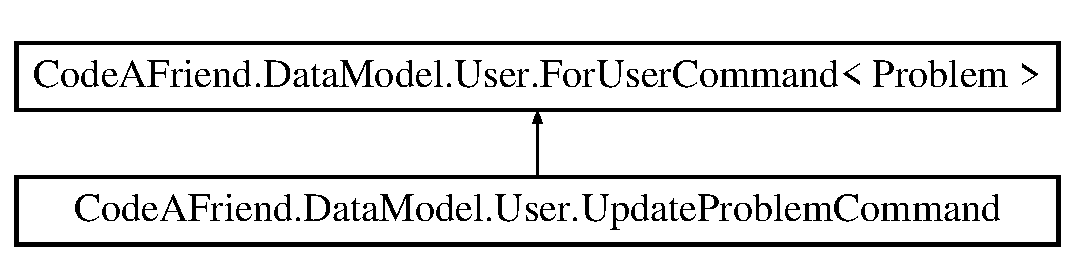
\includegraphics[height=2.000000cm]{class_code_a_friend_1_1_data_model_1_1_user_1_1_update_problem_command}
\end{center}
\end{figure}
\subsection*{Public Member Functions}
\begin{DoxyCompactItemize}
\item 
\mbox{\hyperlink{class_code_a_friend_1_1_data_model_1_1_user_1_1_update_problem_command_ab479f2e60c03c69f054422fba29c4879}{Update\+Problem\+Command}} (string username, string problem\+Name, string description)
\item 
override async Task$<$ \mbox{\hyperlink{class_code_a_friend_1_1_data_model_1_1_problem}{Problem}} $>$ \mbox{\hyperlink{class_code_a_friend_1_1_data_model_1_1_user_1_1_update_problem_command_ab6deb9c81098f15347a52cff94661c4b}{Execute\+Async}} (Db\+Context context)
\end{DoxyCompactItemize}
\subsection*{Properties}
\begin{DoxyCompactItemize}
\item 
string \mbox{\hyperlink{class_code_a_friend_1_1_data_model_1_1_user_1_1_update_problem_command_a77c694466691a4fc02c1f56a017219fa}{Problem\+Name}}\hspace{0.3cm}{\ttfamily  \mbox{[}get, set\mbox{]}}
\begin{DoxyCompactList}\small\item\em Unique name.\end{DoxyCompactList}\item 
string \mbox{\hyperlink{class_code_a_friend_1_1_data_model_1_1_user_1_1_update_problem_command_a542cc19f5586f32a7b6539d41a091c3b}{Description}}\hspace{0.3cm}{\ttfamily  \mbox{[}get, set\mbox{]}}
\begin{DoxyCompactList}\small\item\em Description of the \mbox{\hyperlink{class_code_a_friend_1_1_data_model_1_1_problem}{Problem}}.\end{DoxyCompactList}\end{DoxyCompactItemize}
\subsection*{Additional Inherited Members}


\subsection{Detailed Description}


\subsection{Constructor \& Destructor Documentation}
\mbox{\Hypertarget{class_code_a_friend_1_1_data_model_1_1_user_1_1_update_problem_command_ab479f2e60c03c69f054422fba29c4879}\label{class_code_a_friend_1_1_data_model_1_1_user_1_1_update_problem_command_ab479f2e60c03c69f054422fba29c4879}} 
\index{Code\+A\+Friend\+::\+Data\+Model\+::\+User\+::\+Update\+Problem\+Command@{Code\+A\+Friend\+::\+Data\+Model\+::\+User\+::\+Update\+Problem\+Command}!Update\+Problem\+Command@{Update\+Problem\+Command}}
\index{Update\+Problem\+Command@{Update\+Problem\+Command}!Code\+A\+Friend\+::\+Data\+Model\+::\+User\+::\+Update\+Problem\+Command@{Code\+A\+Friend\+::\+Data\+Model\+::\+User\+::\+Update\+Problem\+Command}}
\subsubsection{\texorpdfstring{Update\+Problem\+Command()}{UpdateProblemCommand()}}
{\footnotesize\ttfamily Code\+A\+Friend.\+Data\+Model.\+User.\+Update\+Problem\+Command.\+Update\+Problem\+Command (\begin{DoxyParamCaption}\item[{string}]{username,  }\item[{string}]{problem\+Name,  }\item[{string}]{description }\end{DoxyParamCaption})}







\subsection{Member Function Documentation}
\mbox{\Hypertarget{class_code_a_friend_1_1_data_model_1_1_user_1_1_update_problem_command_ab6deb9c81098f15347a52cff94661c4b}\label{class_code_a_friend_1_1_data_model_1_1_user_1_1_update_problem_command_ab6deb9c81098f15347a52cff94661c4b}} 
\index{Code\+A\+Friend\+::\+Data\+Model\+::\+User\+::\+Update\+Problem\+Command@{Code\+A\+Friend\+::\+Data\+Model\+::\+User\+::\+Update\+Problem\+Command}!Execute\+Async@{Execute\+Async}}
\index{Execute\+Async@{Execute\+Async}!Code\+A\+Friend\+::\+Data\+Model\+::\+User\+::\+Update\+Problem\+Command@{Code\+A\+Friend\+::\+Data\+Model\+::\+User\+::\+Update\+Problem\+Command}}
\subsubsection{\texorpdfstring{Execute\+Async()}{ExecuteAsync()}}
{\footnotesize\ttfamily override async Task$<$\mbox{\hyperlink{class_code_a_friend_1_1_data_model_1_1_problem}{Problem}}$>$ Code\+A\+Friend.\+Data\+Model.\+User.\+Update\+Problem\+Command.\+Execute\+Async (\begin{DoxyParamCaption}\item[{Db\+Context}]{context }\end{DoxyParamCaption})\hspace{0.3cm}{\ttfamily [virtual]}}







Implements \mbox{\hyperlink{class_code_a_friend_1_1_data_model_1_1_user_1_1_for_user_command_aa9abf9da11dd2a573d8ed93bcf53f6df}{Code\+A\+Friend.\+Data\+Model.\+User.\+For\+User\+Command$<$ Problem $>$}}.



\subsection{Property Documentation}
\mbox{\Hypertarget{class_code_a_friend_1_1_data_model_1_1_user_1_1_update_problem_command_a542cc19f5586f32a7b6539d41a091c3b}\label{class_code_a_friend_1_1_data_model_1_1_user_1_1_update_problem_command_a542cc19f5586f32a7b6539d41a091c3b}} 
\index{Code\+A\+Friend\+::\+Data\+Model\+::\+User\+::\+Update\+Problem\+Command@{Code\+A\+Friend\+::\+Data\+Model\+::\+User\+::\+Update\+Problem\+Command}!Description@{Description}}
\index{Description@{Description}!Code\+A\+Friend\+::\+Data\+Model\+::\+User\+::\+Update\+Problem\+Command@{Code\+A\+Friend\+::\+Data\+Model\+::\+User\+::\+Update\+Problem\+Command}}
\subsubsection{\texorpdfstring{Description}{Description}}
{\footnotesize\ttfamily string Code\+A\+Friend.\+Data\+Model.\+User.\+Update\+Problem\+Command.\+Description\hspace{0.3cm}{\ttfamily [get]}, {\ttfamily [set]}}



Description of the \mbox{\hyperlink{class_code_a_friend_1_1_data_model_1_1_problem}{Problem}}.

\mbox{\Hypertarget{class_code_a_friend_1_1_data_model_1_1_user_1_1_update_problem_command_a77c694466691a4fc02c1f56a017219fa}\label{class_code_a_friend_1_1_data_model_1_1_user_1_1_update_problem_command_a77c694466691a4fc02c1f56a017219fa}} 
\index{Code\+A\+Friend\+::\+Data\+Model\+::\+User\+::\+Update\+Problem\+Command@{Code\+A\+Friend\+::\+Data\+Model\+::\+User\+::\+Update\+Problem\+Command}!Problem\+Name@{Problem\+Name}}
\index{Problem\+Name@{Problem\+Name}!Code\+A\+Friend\+::\+Data\+Model\+::\+User\+::\+Update\+Problem\+Command@{Code\+A\+Friend\+::\+Data\+Model\+::\+User\+::\+Update\+Problem\+Command}}
\subsubsection{\texorpdfstring{Problem\+Name}{ProblemName}}
{\footnotesize\ttfamily string Code\+A\+Friend.\+Data\+Model.\+User.\+Update\+Problem\+Command.\+Problem\+Name\hspace{0.3cm}{\ttfamily [get]}, {\ttfamily [set]}}



Unique name.



The documentation for this class was generated from the following file\+:\begin{DoxyCompactItemize}
\item 
shared/\+Code\+A\+Friend.\+Data\+Model/\+User\+Logic/\mbox{\hyperlink{_user_8_problem_commands_8cs}{User.\+Problem\+Commands.\+cs}}\end{DoxyCompactItemize}

\hypertarget{class_code_a_friend_1_1_data_model_1_1_user_1_1_update_script_command}{}\section{Code\+A\+Friend.\+Data\+Model.\+User.\+Update\+Script\+Command Class Reference}
\label{class_code_a_friend_1_1_data_model_1_1_user_1_1_update_script_command}\index{Code\+A\+Friend.\+Data\+Model.\+User.\+Update\+Script\+Command@{Code\+A\+Friend.\+Data\+Model.\+User.\+Update\+Script\+Command}}


 


Inheritance diagram for Code\+A\+Friend.\+Data\+Model.\+User.\+Update\+Script\+Command\+:\begin{figure}[H]
\begin{center}
\leavevmode
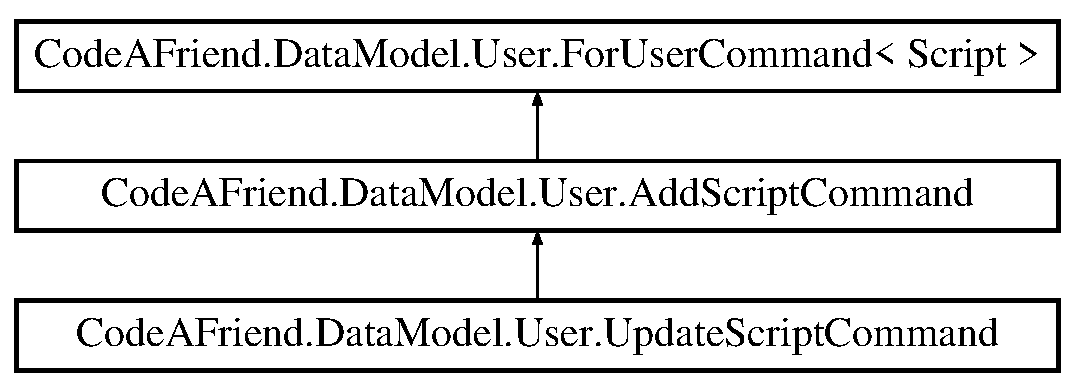
\includegraphics[height=3.000000cm]{class_code_a_friend_1_1_data_model_1_1_user_1_1_update_script_command}
\end{center}
\end{figure}
\subsection*{Public Member Functions}
\begin{DoxyCompactItemize}
\item 
\mbox{\hyperlink{class_code_a_friend_1_1_data_model_1_1_user_1_1_update_script_command_a4cf4c6d1cbdb87cba9b4c38fb5b0e900}{Update\+Script\+Command}} (Guid script\+Id, string username, string name, string body, \mbox{\hyperlink{namespace_code_a_friend_1_1_data_model_a13e088c525db1b03a4de75420ced79b2}{Supported\+Language}} language)
\item 
override async Task$<$ \mbox{\hyperlink{class_code_a_friend_1_1_data_model_1_1_script}{Script}} $>$ \mbox{\hyperlink{class_code_a_friend_1_1_data_model_1_1_user_1_1_update_script_command_a54e74e6d68bfc5e01cbcc96fd6dfbd2d}{Execute\+Async}} (Db\+Context context)
\end{DoxyCompactItemize}
\subsection*{Properties}
\begin{DoxyCompactItemize}
\item 
Guid \mbox{\hyperlink{class_code_a_friend_1_1_data_model_1_1_user_1_1_update_script_command_a5f8fe92856201f191887693214d7383f}{Script\+Id}}\hspace{0.3cm}{\ttfamily  \mbox{[}get, set\mbox{]}}
\begin{DoxyCompactList}\small\item\em Id of the \mbox{\hyperlink{class_code_a_friend_1_1_data_model_1_1_script}{Script}} to operate on.\end{DoxyCompactList}\end{DoxyCompactItemize}
\subsection*{Additional Inherited Members}


\subsection{Detailed Description}


\subsection{Constructor \& Destructor Documentation}
\mbox{\Hypertarget{class_code_a_friend_1_1_data_model_1_1_user_1_1_update_script_command_a4cf4c6d1cbdb87cba9b4c38fb5b0e900}\label{class_code_a_friend_1_1_data_model_1_1_user_1_1_update_script_command_a4cf4c6d1cbdb87cba9b4c38fb5b0e900}} 
\index{Code\+A\+Friend\+::\+Data\+Model\+::\+User\+::\+Update\+Script\+Command@{Code\+A\+Friend\+::\+Data\+Model\+::\+User\+::\+Update\+Script\+Command}!Update\+Script\+Command@{Update\+Script\+Command}}
\index{Update\+Script\+Command@{Update\+Script\+Command}!Code\+A\+Friend\+::\+Data\+Model\+::\+User\+::\+Update\+Script\+Command@{Code\+A\+Friend\+::\+Data\+Model\+::\+User\+::\+Update\+Script\+Command}}
\subsubsection{\texorpdfstring{Update\+Script\+Command()}{UpdateScriptCommand()}}
{\footnotesize\ttfamily Code\+A\+Friend.\+Data\+Model.\+User.\+Update\+Script\+Command.\+Update\+Script\+Command (\begin{DoxyParamCaption}\item[{Guid}]{script\+Id,  }\item[{string}]{username,  }\item[{string}]{name,  }\item[{string}]{body,  }\item[{\mbox{\hyperlink{namespace_code_a_friend_1_1_data_model_a13e088c525db1b03a4de75420ced79b2}{Supported\+Language}}}]{language }\end{DoxyParamCaption})}







\subsection{Member Function Documentation}
\mbox{\Hypertarget{class_code_a_friend_1_1_data_model_1_1_user_1_1_update_script_command_a54e74e6d68bfc5e01cbcc96fd6dfbd2d}\label{class_code_a_friend_1_1_data_model_1_1_user_1_1_update_script_command_a54e74e6d68bfc5e01cbcc96fd6dfbd2d}} 
\index{Code\+A\+Friend\+::\+Data\+Model\+::\+User\+::\+Update\+Script\+Command@{Code\+A\+Friend\+::\+Data\+Model\+::\+User\+::\+Update\+Script\+Command}!Execute\+Async@{Execute\+Async}}
\index{Execute\+Async@{Execute\+Async}!Code\+A\+Friend\+::\+Data\+Model\+::\+User\+::\+Update\+Script\+Command@{Code\+A\+Friend\+::\+Data\+Model\+::\+User\+::\+Update\+Script\+Command}}
\subsubsection{\texorpdfstring{Execute\+Async()}{ExecuteAsync()}}
{\footnotesize\ttfamily override async Task$<$\mbox{\hyperlink{class_code_a_friend_1_1_data_model_1_1_script}{Script}}$>$ Code\+A\+Friend.\+Data\+Model.\+User.\+Update\+Script\+Command.\+Execute\+Async (\begin{DoxyParamCaption}\item[{Db\+Context}]{context }\end{DoxyParamCaption})\hspace{0.3cm}{\ttfamily [virtual]}}







Reimplemented from \mbox{\hyperlink{class_code_a_friend_1_1_data_model_1_1_user_1_1_add_script_command_a7105f586c7502c18a3ac2cfd567c90f0}{Code\+A\+Friend.\+Data\+Model.\+User.\+Add\+Script\+Command}}.



\subsection{Property Documentation}
\mbox{\Hypertarget{class_code_a_friend_1_1_data_model_1_1_user_1_1_update_script_command_a5f8fe92856201f191887693214d7383f}\label{class_code_a_friend_1_1_data_model_1_1_user_1_1_update_script_command_a5f8fe92856201f191887693214d7383f}} 
\index{Code\+A\+Friend\+::\+Data\+Model\+::\+User\+::\+Update\+Script\+Command@{Code\+A\+Friend\+::\+Data\+Model\+::\+User\+::\+Update\+Script\+Command}!Script\+Id@{Script\+Id}}
\index{Script\+Id@{Script\+Id}!Code\+A\+Friend\+::\+Data\+Model\+::\+User\+::\+Update\+Script\+Command@{Code\+A\+Friend\+::\+Data\+Model\+::\+User\+::\+Update\+Script\+Command}}
\subsubsection{\texorpdfstring{Script\+Id}{ScriptId}}
{\footnotesize\ttfamily Guid Code\+A\+Friend.\+Data\+Model.\+User.\+Update\+Script\+Command.\+Script\+Id\hspace{0.3cm}{\ttfamily [get]}, {\ttfamily [set]}}



Id of the \mbox{\hyperlink{class_code_a_friend_1_1_data_model_1_1_script}{Script}} to operate on.



The documentation for this class was generated from the following file\+:\begin{DoxyCompactItemize}
\item 
shared/\+Code\+A\+Friend.\+Data\+Model/\+User\+Logic/\mbox{\hyperlink{_user_8_script_commands_8cs}{User.\+Script\+Commands.\+cs}}\end{DoxyCompactItemize}

\hypertarget{class_code_a_friend_1_1_data_model_1_1_user}{}\section{Code\+A\+Friend.\+Data\+Model.\+User Class Reference}
\label{class_code_a_friend_1_1_data_model_1_1_user}\index{Code\+A\+Friend.\+Data\+Model.\+User@{Code\+A\+Friend.\+Data\+Model.\+User}}


\mbox{\hyperlink{class_code_a_friend_1_1_data_model_1_1_user}{User}} in the \mbox{\hyperlink{namespace_code_a_friend}{Code\+A\+Friend}} system. 


\subsection*{Classes}
\begin{DoxyCompactItemize}
\item 
class \mbox{\hyperlink{class_code_a_friend_1_1_data_model_1_1_user_1_1_add_problem_command}{Add\+Problem\+Command}}
\begin{DoxyCompactList}\small\item\em Properties someone can specify on \mbox{\hyperlink{class_code_a_friend_1_1_data_model_1_1_problem}{Problem}} creation.\end{DoxyCompactList}\item 
class \mbox{\hyperlink{class_code_a_friend_1_1_data_model_1_1_user_1_1_add_script_command}{Add\+Script\+Command}}
\begin{DoxyCompactList}\small\item\em Properties someone can specify on script creation.\end{DoxyCompactList}\item 
class \mbox{\hyperlink{class_code_a_friend_1_1_data_model_1_1_user_1_1_create_command}{Create\+Command}}
\begin{DoxyCompactList}\small\item\em Properties someone can specify on user creation.\end{DoxyCompactList}\item 
class \mbox{\hyperlink{class_code_a_friend_1_1_data_model_1_1_user_1_1_delete_problem_command}{Delete\+Problem\+Command}}
\item 
class \mbox{\hyperlink{class_code_a_friend_1_1_data_model_1_1_user_1_1_delete_script_command}{Delete\+Script\+Command}}
\item 
class \mbox{\hyperlink{class_code_a_friend_1_1_data_model_1_1_user_1_1_for_user_command}{For\+User\+Command}}
\begin{DoxyCompactList}\small\item\em Command being performed on behalf of a specific user.\end{DoxyCompactList}\item 
class \mbox{\hyperlink{class_code_a_friend_1_1_data_model_1_1_user_1_1_update_problem_command}{Update\+Problem\+Command}}
\item 
class \mbox{\hyperlink{class_code_a_friend_1_1_data_model_1_1_user_1_1_update_script_command}{Update\+Script\+Command}}
\end{DoxyCompactItemize}
\subsection*{Public Member Functions}
\begin{DoxyCompactItemize}
\item 
\mbox{\hyperlink{class_code_a_friend_1_1_data_model_1_1_user_a5604cc5f196cf59ac2b4b036d20b2227}{User}} (string name)
\begin{DoxyCompactList}\small\item\em Constructor for creating new \mbox{\hyperlink{class_code_a_friend_1_1_data_model_1_1_user}{User}}.\end{DoxyCompactList}\item 
async Task$<$ \mbox{\hyperlink{class_code_a_friend_1_1_data_model_1_1_user_script}{User\+Script}} $>$ \mbox{\hyperlink{class_code_a_friend_1_1_data_model_1_1_user_accaaafd48c85875b1d61622c4e58db05}{Add\+Async}} (\mbox{\hyperlink{class_code_a_friend_1_1_data_model_1_1_user_1_1_add_script_command}{Add\+Script\+Command}} script, Db\+Context context=null)
\begin{DoxyCompactList}\small\item\em Add a \mbox{\hyperlink{class_code_a_friend_1_1_data_model_1_1_user_script}{User\+Script}} to this \mbox{\hyperlink{class_code_a_friend_1_1_data_model_1_1_user}{User}}. \end{DoxyCompactList}\item 
async Task$<$ \mbox{\hyperlink{class_code_a_friend_1_1_data_model_1_1_problem}{Problem}} $>$ \mbox{\hyperlink{class_code_a_friend_1_1_data_model_1_1_user_a15aa0e1bb20abcd45da38e11f30bb6e4}{Add\+Async}} (\mbox{\hyperlink{class_code_a_friend_1_1_data_model_1_1_user_1_1_add_problem_command}{Add\+Problem\+Command}} problem, Db\+Context context=null)
\begin{DoxyCompactList}\small\item\em Add a \mbox{\hyperlink{class_code_a_friend_1_1_data_model_1_1_problem}{Problem}} to this \mbox{\hyperlink{class_code_a_friend_1_1_data_model_1_1_user}{User}}. \end{DoxyCompactList}\end{DoxyCompactItemize}
\subsection*{Public Attributes}
\begin{DoxyCompactItemize}
\item 
I\+Enumerable$<$ \mbox{\hyperlink{class_code_a_friend_1_1_data_model_1_1_user_script}{User\+Script}} $>$ \mbox{\hyperlink{class_code_a_friend_1_1_data_model_1_1_user_ae1e8268cdd9f9abffcf602146de030f5}{Scripts}} =$>$ \+\_\+scripts?.To\+List()
\begin{DoxyCompactList}\small\item\em \mbox{\hyperlink{class_code_a_friend_1_1_data_model_1_1_user_script}{User\+Script}}s that this user has written.\end{DoxyCompactList}\item 
I\+Enumerable$<$ \mbox{\hyperlink{class_code_a_friend_1_1_data_model_1_1_problem}{Problem}} $>$ \mbox{\hyperlink{class_code_a_friend_1_1_data_model_1_1_user_afdc167d3127eb8aae3d5754642b6eff0}{Problems}} =$>$ \+\_\+problems?.To\+List()
\begin{DoxyCompactList}\small\item\em \mbox{\hyperlink{class_code_a_friend_1_1_data_model_1_1_problem}{Problem}}s that this user has written.\end{DoxyCompactList}\end{DoxyCompactItemize}
\subsection*{Properties}
\begin{DoxyCompactItemize}
\item 
string \mbox{\hyperlink{class_code_a_friend_1_1_data_model_1_1_user_ab32bf10478eb4276407dd192fa313954}{Name}}\hspace{0.3cm}{\ttfamily  \mbox{[}get\mbox{]}}
\begin{DoxyCompactList}\small\item\em This user\textquotesingle{}s unique name.\end{DoxyCompactList}\end{DoxyCompactItemize}


\subsection{Detailed Description}
\mbox{\hyperlink{class_code_a_friend_1_1_data_model_1_1_user}{User}} in the \mbox{\hyperlink{namespace_code_a_friend}{Code\+A\+Friend}} system.



\subsection{Constructor \& Destructor Documentation}
\mbox{\Hypertarget{class_code_a_friend_1_1_data_model_1_1_user_a5604cc5f196cf59ac2b4b036d20b2227}\label{class_code_a_friend_1_1_data_model_1_1_user_a5604cc5f196cf59ac2b4b036d20b2227}} 
\index{Code\+A\+Friend\+::\+Data\+Model\+::\+User@{Code\+A\+Friend\+::\+Data\+Model\+::\+User}!User@{User}}
\index{User@{User}!Code\+A\+Friend\+::\+Data\+Model\+::\+User@{Code\+A\+Friend\+::\+Data\+Model\+::\+User}}
\subsubsection{\texorpdfstring{User()}{User()}}
{\footnotesize\ttfamily Code\+A\+Friend.\+Data\+Model.\+User.\+User (\begin{DoxyParamCaption}\item[{string}]{name }\end{DoxyParamCaption})}



Constructor for creating new \mbox{\hyperlink{class_code_a_friend_1_1_data_model_1_1_user}{User}}.



\subsection{Member Function Documentation}
\mbox{\Hypertarget{class_code_a_friend_1_1_data_model_1_1_user_accaaafd48c85875b1d61622c4e58db05}\label{class_code_a_friend_1_1_data_model_1_1_user_accaaafd48c85875b1d61622c4e58db05}} 
\index{Code\+A\+Friend\+::\+Data\+Model\+::\+User@{Code\+A\+Friend\+::\+Data\+Model\+::\+User}!Add\+Async@{Add\+Async}}
\index{Add\+Async@{Add\+Async}!Code\+A\+Friend\+::\+Data\+Model\+::\+User@{Code\+A\+Friend\+::\+Data\+Model\+::\+User}}
\subsubsection{\texorpdfstring{Add\+Async()}{AddAsync()}\hspace{0.1cm}{\footnotesize\ttfamily [1/2]}}
{\footnotesize\ttfamily async Task$<$\mbox{\hyperlink{class_code_a_friend_1_1_data_model_1_1_user_script}{User\+Script}}$>$ Code\+A\+Friend.\+Data\+Model.\+User.\+Add\+Async (\begin{DoxyParamCaption}\item[{\mbox{\hyperlink{class_code_a_friend_1_1_data_model_1_1_user_1_1_add_script_command}{Add\+Script\+Command}}}]{script,  }\item[{Db\+Context}]{context = {\ttfamily null} }\end{DoxyParamCaption})}



Add a \mbox{\hyperlink{class_code_a_friend_1_1_data_model_1_1_user_script}{User\+Script}} to this \mbox{\hyperlink{class_code_a_friend_1_1_data_model_1_1_user}{User}}. 


\begin{DoxyParams}{Parameters}
{\em script} & \mbox{\hyperlink{class_code_a_friend_1_1_data_model_1_1_user_script}{User\+Script}} to add.\\
\hline
{\em context} & Database to save the updated state to. (When Save\+Changes is called).\\
\hline
\end{DoxyParams}
\mbox{\Hypertarget{class_code_a_friend_1_1_data_model_1_1_user_a15aa0e1bb20abcd45da38e11f30bb6e4}\label{class_code_a_friend_1_1_data_model_1_1_user_a15aa0e1bb20abcd45da38e11f30bb6e4}} 
\index{Code\+A\+Friend\+::\+Data\+Model\+::\+User@{Code\+A\+Friend\+::\+Data\+Model\+::\+User}!Add\+Async@{Add\+Async}}
\index{Add\+Async@{Add\+Async}!Code\+A\+Friend\+::\+Data\+Model\+::\+User@{Code\+A\+Friend\+::\+Data\+Model\+::\+User}}
\subsubsection{\texorpdfstring{Add\+Async()}{AddAsync()}\hspace{0.1cm}{\footnotesize\ttfamily [2/2]}}
{\footnotesize\ttfamily async Task$<$\mbox{\hyperlink{class_code_a_friend_1_1_data_model_1_1_problem}{Problem}}$>$ Code\+A\+Friend.\+Data\+Model.\+User.\+Add\+Async (\begin{DoxyParamCaption}\item[{\mbox{\hyperlink{class_code_a_friend_1_1_data_model_1_1_user_1_1_add_problem_command}{Add\+Problem\+Command}}}]{problem,  }\item[{Db\+Context}]{context = {\ttfamily null} }\end{DoxyParamCaption})}



Add a \mbox{\hyperlink{class_code_a_friend_1_1_data_model_1_1_problem}{Problem}} to this \mbox{\hyperlink{class_code_a_friend_1_1_data_model_1_1_user}{User}}. 


\begin{DoxyParams}{Parameters}
{\em problem} & \mbox{\hyperlink{class_code_a_friend_1_1_data_model_1_1_problem}{Problem}} to add.\\
\hline
{\em context} & Database to save the updated state to. (When Save\+Changes is called).\\
\hline
\end{DoxyParams}


\subsection{Member Data Documentation}
\mbox{\Hypertarget{class_code_a_friend_1_1_data_model_1_1_user_afdc167d3127eb8aae3d5754642b6eff0}\label{class_code_a_friend_1_1_data_model_1_1_user_afdc167d3127eb8aae3d5754642b6eff0}} 
\index{Code\+A\+Friend\+::\+Data\+Model\+::\+User@{Code\+A\+Friend\+::\+Data\+Model\+::\+User}!Problems@{Problems}}
\index{Problems@{Problems}!Code\+A\+Friend\+::\+Data\+Model\+::\+User@{Code\+A\+Friend\+::\+Data\+Model\+::\+User}}
\subsubsection{\texorpdfstring{Problems}{Problems}}
{\footnotesize\ttfamily I\+Enumerable$<$\mbox{\hyperlink{class_code_a_friend_1_1_data_model_1_1_problem}{Problem}}$>$ Code\+A\+Friend.\+Data\+Model.\+User.\+Problems =$>$ \+\_\+problems?.To\+List()}



\mbox{\hyperlink{class_code_a_friend_1_1_data_model_1_1_problem}{Problem}}s that this user has written.

\mbox{\Hypertarget{class_code_a_friend_1_1_data_model_1_1_user_ae1e8268cdd9f9abffcf602146de030f5}\label{class_code_a_friend_1_1_data_model_1_1_user_ae1e8268cdd9f9abffcf602146de030f5}} 
\index{Code\+A\+Friend\+::\+Data\+Model\+::\+User@{Code\+A\+Friend\+::\+Data\+Model\+::\+User}!Scripts@{Scripts}}
\index{Scripts@{Scripts}!Code\+A\+Friend\+::\+Data\+Model\+::\+User@{Code\+A\+Friend\+::\+Data\+Model\+::\+User}}
\subsubsection{\texorpdfstring{Scripts}{Scripts}}
{\footnotesize\ttfamily I\+Enumerable$<$\mbox{\hyperlink{class_code_a_friend_1_1_data_model_1_1_user_script}{User\+Script}}$>$ Code\+A\+Friend.\+Data\+Model.\+User.\+Scripts =$>$ \+\_\+scripts?.To\+List()}



\mbox{\hyperlink{class_code_a_friend_1_1_data_model_1_1_user_script}{User\+Script}}s that this user has written.



\subsection{Property Documentation}
\mbox{\Hypertarget{class_code_a_friend_1_1_data_model_1_1_user_ab32bf10478eb4276407dd192fa313954}\label{class_code_a_friend_1_1_data_model_1_1_user_ab32bf10478eb4276407dd192fa313954}} 
\index{Code\+A\+Friend\+::\+Data\+Model\+::\+User@{Code\+A\+Friend\+::\+Data\+Model\+::\+User}!Name@{Name}}
\index{Name@{Name}!Code\+A\+Friend\+::\+Data\+Model\+::\+User@{Code\+A\+Friend\+::\+Data\+Model\+::\+User}}
\subsubsection{\texorpdfstring{Name}{Name}}
{\footnotesize\ttfamily string Code\+A\+Friend.\+Data\+Model.\+User.\+Name\hspace{0.3cm}{\ttfamily [get]}}



This user\textquotesingle{}s unique name.



The documentation for this class was generated from the following files\+:\begin{DoxyCompactItemize}
\item 
shared/\+Code\+A\+Friend.\+Data\+Model/\+User\+Logic/\mbox{\hyperlink{_user_8_commands_8cs}{User.\+Commands.\+cs}}\item 
shared/\+Code\+A\+Friend.\+Data\+Model/\+User\+Logic/\mbox{\hyperlink{_user_8cs}{User.\+cs}}\end{DoxyCompactItemize}

\hypertarget{class_code_a_friend_1_1_api_service_1_1_controllers_1_1_user_controller}{}\section{Code\+A\+Friend.\+Api\+Service.\+Controllers.\+User\+Controller Class Reference}
\label{class_code_a_friend_1_1_api_service_1_1_controllers_1_1_user_controller}\index{Code\+A\+Friend.\+Api\+Service.\+Controllers.\+User\+Controller@{Code\+A\+Friend.\+Api\+Service.\+Controllers.\+User\+Controller}}


 


Inheritance diagram for Code\+A\+Friend.\+Api\+Service.\+Controllers.\+User\+Controller\+:\begin{figure}[H]
\begin{center}
\leavevmode
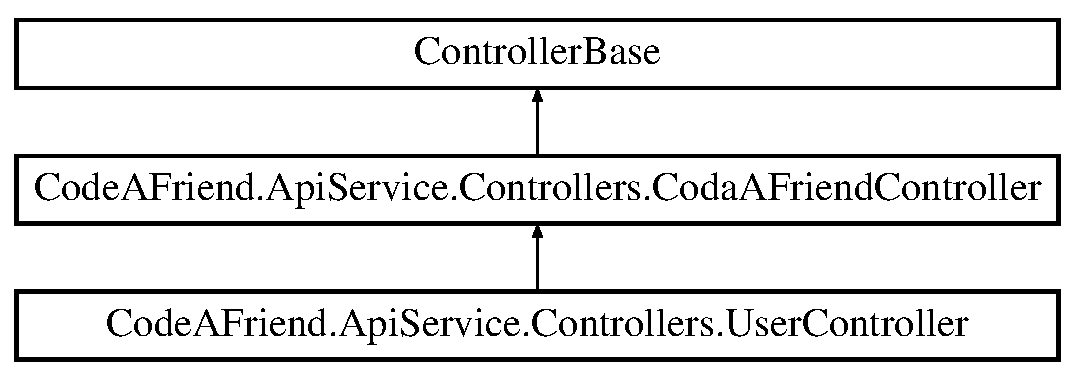
\includegraphics[height=3.000000cm]{class_code_a_friend_1_1_api_service_1_1_controllers_1_1_user_controller}
\end{center}
\end{figure}
\subsection*{Public Member Functions}
\begin{DoxyCompactItemize}
\item 
\mbox{\hyperlink{class_code_a_friend_1_1_api_service_1_1_controllers_1_1_user_controller_a62af772aa676edcc545ffb0aa0cb9bc9}{User\+Controller}} (\mbox{\hyperlink{interface_code_a_friend_1_1_facade_1_1_i_code_a_friend_facade}{I\+Code\+A\+Friend\+Facade}} facade)
\item 
async Task$<$ I\+Action\+Result $>$ \mbox{\hyperlink{class_code_a_friend_1_1_api_service_1_1_controllers_1_1_user_controller_acd97e404e641c3acfe8a0b5d4a34e4ef}{Create}} (\mbox{\hyperlink{class_code_a_friend_1_1_data_model_1_1_user_1_1_create_command}{User.\+Create\+Command}} command)
\begin{DoxyCompactList}\small\item\em Create a new user. \end{DoxyCompactList}\item 
async Task$<$ I\+Action\+Result $>$ \mbox{\hyperlink{class_code_a_friend_1_1_api_service_1_1_controllers_1_1_user_controller_aa4579aedefb04bb5916153a2bb9f42a2}{Get\+User}} (string username)
\begin{DoxyCompactList}\small\item\em Get a user by username. \end{DoxyCompactList}\item 
async Task$<$ I\+Action\+Result $>$ \mbox{\hyperlink{class_code_a_friend_1_1_api_service_1_1_controllers_1_1_user_controller_a2bcc77065fde0735cf40b6cb38ce97d3}{Get\+Scripts}} (string username)
\begin{DoxyCompactList}\small\item\em Get all of a user\textquotesingle{}s scripts. \end{DoxyCompactList}\end{DoxyCompactItemize}
\subsection*{Additional Inherited Members}


\subsection{Detailed Description}




\subsection{Constructor \& Destructor Documentation}
\mbox{\Hypertarget{class_code_a_friend_1_1_api_service_1_1_controllers_1_1_user_controller_a62af772aa676edcc545ffb0aa0cb9bc9}\label{class_code_a_friend_1_1_api_service_1_1_controllers_1_1_user_controller_a62af772aa676edcc545ffb0aa0cb9bc9}} 
\index{Code\+A\+Friend\+::\+Api\+Service\+::\+Controllers\+::\+User\+Controller@{Code\+A\+Friend\+::\+Api\+Service\+::\+Controllers\+::\+User\+Controller}!User\+Controller@{User\+Controller}}
\index{User\+Controller@{User\+Controller}!Code\+A\+Friend\+::\+Api\+Service\+::\+Controllers\+::\+User\+Controller@{Code\+A\+Friend\+::\+Api\+Service\+::\+Controllers\+::\+User\+Controller}}
\subsubsection{\texorpdfstring{User\+Controller()}{UserController()}}
{\footnotesize\ttfamily Code\+A\+Friend.\+Api\+Service.\+Controllers.\+User\+Controller.\+User\+Controller (\begin{DoxyParamCaption}\item[{\mbox{\hyperlink{interface_code_a_friend_1_1_facade_1_1_i_code_a_friend_facade}{I\+Code\+A\+Friend\+Facade}}}]{facade }\end{DoxyParamCaption})}







\subsection{Member Function Documentation}
\mbox{\Hypertarget{class_code_a_friend_1_1_api_service_1_1_controllers_1_1_user_controller_acd97e404e641c3acfe8a0b5d4a34e4ef}\label{class_code_a_friend_1_1_api_service_1_1_controllers_1_1_user_controller_acd97e404e641c3acfe8a0b5d4a34e4ef}} 
\index{Code\+A\+Friend\+::\+Api\+Service\+::\+Controllers\+::\+User\+Controller@{Code\+A\+Friend\+::\+Api\+Service\+::\+Controllers\+::\+User\+Controller}!Create@{Create}}
\index{Create@{Create}!Code\+A\+Friend\+::\+Api\+Service\+::\+Controllers\+::\+User\+Controller@{Code\+A\+Friend\+::\+Api\+Service\+::\+Controllers\+::\+User\+Controller}}
\subsubsection{\texorpdfstring{Create()}{Create()}}
{\footnotesize\ttfamily async Task$<$I\+Action\+Result$>$ Code\+A\+Friend.\+Api\+Service.\+Controllers.\+User\+Controller.\+Create (\begin{DoxyParamCaption}\item[{\mbox{\hyperlink{class_code_a_friend_1_1_data_model_1_1_user_1_1_create_command}{User.\+Create\+Command}}}]{command }\end{DoxyParamCaption})}



Create a new user. 


\begin{DoxyParams}{Parameters}
{\em command} & command to create a new User.\\
\hline
\end{DoxyParams}
\begin{DoxyReturn}{Returns}
Created User and the uri where it now resides.
\end{DoxyReturn}
\mbox{\Hypertarget{class_code_a_friend_1_1_api_service_1_1_controllers_1_1_user_controller_a2bcc77065fde0735cf40b6cb38ce97d3}\label{class_code_a_friend_1_1_api_service_1_1_controllers_1_1_user_controller_a2bcc77065fde0735cf40b6cb38ce97d3}} 
\index{Code\+A\+Friend\+::\+Api\+Service\+::\+Controllers\+::\+User\+Controller@{Code\+A\+Friend\+::\+Api\+Service\+::\+Controllers\+::\+User\+Controller}!Get\+Scripts@{Get\+Scripts}}
\index{Get\+Scripts@{Get\+Scripts}!Code\+A\+Friend\+::\+Api\+Service\+::\+Controllers\+::\+User\+Controller@{Code\+A\+Friend\+::\+Api\+Service\+::\+Controllers\+::\+User\+Controller}}
\subsubsection{\texorpdfstring{Get\+Scripts()}{GetScripts()}}
{\footnotesize\ttfamily async Task$<$I\+Action\+Result$>$ Code\+A\+Friend.\+Api\+Service.\+Controllers.\+User\+Controller.\+Get\+Scripts (\begin{DoxyParamCaption}\item[{string}]{username }\end{DoxyParamCaption})}



Get all of a user\textquotesingle{}s scripts. 


\begin{DoxyParams}{Parameters}
{\em username} & \\
\hline
\end{DoxyParams}
\begin{DoxyReturn}{Returns}
I\+Enumerable$<$\+Script$>$
\end{DoxyReturn}
\mbox{\Hypertarget{class_code_a_friend_1_1_api_service_1_1_controllers_1_1_user_controller_aa4579aedefb04bb5916153a2bb9f42a2}\label{class_code_a_friend_1_1_api_service_1_1_controllers_1_1_user_controller_aa4579aedefb04bb5916153a2bb9f42a2}} 
\index{Code\+A\+Friend\+::\+Api\+Service\+::\+Controllers\+::\+User\+Controller@{Code\+A\+Friend\+::\+Api\+Service\+::\+Controllers\+::\+User\+Controller}!Get\+User@{Get\+User}}
\index{Get\+User@{Get\+User}!Code\+A\+Friend\+::\+Api\+Service\+::\+Controllers\+::\+User\+Controller@{Code\+A\+Friend\+::\+Api\+Service\+::\+Controllers\+::\+User\+Controller}}
\subsubsection{\texorpdfstring{Get\+User()}{GetUser()}}
{\footnotesize\ttfamily async Task$<$I\+Action\+Result$>$ Code\+A\+Friend.\+Api\+Service.\+Controllers.\+User\+Controller.\+Get\+User (\begin{DoxyParamCaption}\item[{string}]{username }\end{DoxyParamCaption})}



Get a user by username. 


\begin{DoxyParams}{Parameters}
{\em username} & user\textquotesingle{}s username\\
\hline
\end{DoxyParams}
\begin{DoxyReturn}{Returns}
User
\end{DoxyReturn}


The documentation for this class was generated from the following file\+:\begin{DoxyCompactItemize}
\item 
apps/\+Code\+A\+Friend.\+Api\+Service/\+Controllers/\mbox{\hyperlink{_user_controller_8cs}{User\+Controller.\+cs}}\end{DoxyCompactItemize}

\hypertarget{class_code_a_friend_1_1_data_model_1_1_user_script}{}\section{Code\+A\+Friend.\+Data\+Model.\+User\+Script Class Reference}
\label{class_code_a_friend_1_1_data_model_1_1_user_script}\index{Code\+A\+Friend.\+Data\+Model.\+User\+Script@{Code\+A\+Friend.\+Data\+Model.\+User\+Script}}


A \mbox{\hyperlink{class_code_a_friend_1_1_data_model_1_1_script}{Script}} that belongs to a specific user.  


Inheritance diagram for Code\+A\+Friend.\+Data\+Model.\+User\+Script\+:\begin{figure}[H]
\begin{center}
\leavevmode
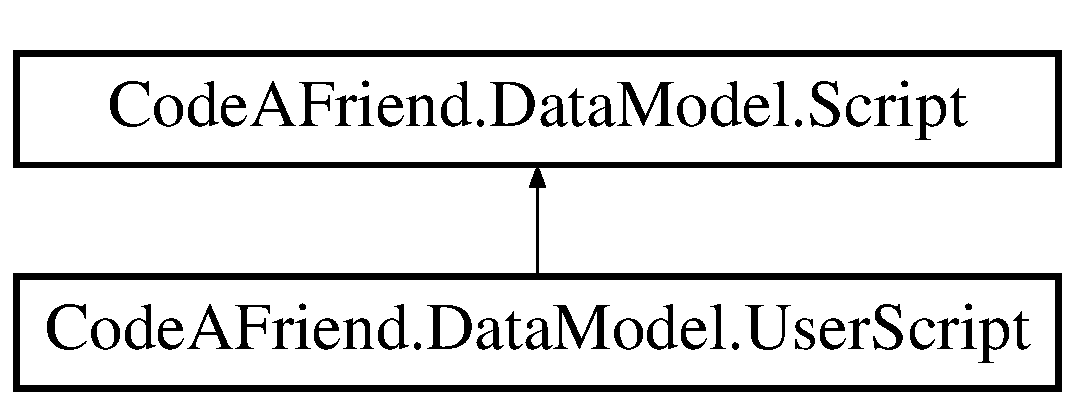
\includegraphics[height=2.000000cm]{class_code_a_friend_1_1_data_model_1_1_user_script}
\end{center}
\end{figure}
\subsection*{Public Member Functions}
\begin{DoxyCompactItemize}
\item 
\mbox{\hyperlink{class_code_a_friend_1_1_data_model_1_1_user_script_a2d9bbf3cdb8d330b15c7bb18f9b5c145}{User\+Script}} (string name, string body, \mbox{\hyperlink{namespace_code_a_friend_1_1_data_model_a13e088c525db1b03a4de75420ced79b2}{Supported\+Language}} language)
\begin{DoxyCompactList}\small\item\em Constructor for creating new \mbox{\hyperlink{class_code_a_friend_1_1_data_model_1_1_user_script}{User\+Script}}.\end{DoxyCompactList}\end{DoxyCompactItemize}
\subsection*{Additional Inherited Members}


\subsection{Detailed Description}
A \mbox{\hyperlink{class_code_a_friend_1_1_data_model_1_1_script}{Script}} that belongs to a specific user. 



\subsection{Constructor \& Destructor Documentation}
\mbox{\Hypertarget{class_code_a_friend_1_1_data_model_1_1_user_script_a2d9bbf3cdb8d330b15c7bb18f9b5c145}\label{class_code_a_friend_1_1_data_model_1_1_user_script_a2d9bbf3cdb8d330b15c7bb18f9b5c145}} 
\index{Code\+A\+Friend\+::\+Data\+Model\+::\+User\+Script@{Code\+A\+Friend\+::\+Data\+Model\+::\+User\+Script}!User\+Script@{User\+Script}}
\index{User\+Script@{User\+Script}!Code\+A\+Friend\+::\+Data\+Model\+::\+User\+Script@{Code\+A\+Friend\+::\+Data\+Model\+::\+User\+Script}}
\subsubsection{\texorpdfstring{User\+Script()}{UserScript()}}
{\footnotesize\ttfamily Code\+A\+Friend.\+Data\+Model.\+User\+Script.\+User\+Script (\begin{DoxyParamCaption}\item[{string}]{name,  }\item[{string}]{body,  }\item[{\mbox{\hyperlink{namespace_code_a_friend_1_1_data_model_a13e088c525db1b03a4de75420ced79b2}{Supported\+Language}}}]{language }\end{DoxyParamCaption})}



Constructor for creating new \mbox{\hyperlink{class_code_a_friend_1_1_data_model_1_1_user_script}{User\+Script}}.



The documentation for this class was generated from the following file\+:\begin{DoxyCompactItemize}
\item 
shared/\+Code\+A\+Friend.\+Data\+Model/\+User\+Logic/\mbox{\hyperlink{_user_script_8cs}{User\+Script.\+cs}}\end{DoxyCompactItemize}

\hypertarget{class_code_a_friend_1_1_data_model_1_1_vote}{}\section{Code\+A\+Friend.\+Data\+Model.\+Vote Class Reference}
\label{class_code_a_friend_1_1_data_model_1_1_vote}\index{Code\+A\+Friend.\+Data\+Model.\+Vote@{Code\+A\+Friend.\+Data\+Model.\+Vote}}


\mbox{\hyperlink{class_code_a_friend_1_1_data_model_1_1_vote}{Vote}} for the value for a specific \mbox{\hyperlink{class_code_a_friend_1_1_data_model_1_1_problem_solution}{Problem\+Solution}}.  


\subsection*{Public Member Functions}
\begin{DoxyCompactItemize}
\item 
\mbox{\hyperlink{class_code_a_friend_1_1_data_model_1_1_vote_ac4cd3a11d8dfa4ea9051393dc9a5fa72}{Vote}} (short value, \mbox{\hyperlink{class_code_a_friend_1_1_data_model_1_1_user}{User}} submitter, string comment)
\begin{DoxyCompactList}\small\item\em Constructor for creating new \mbox{\hyperlink{class_code_a_friend_1_1_data_model_1_1_vote}{Vote}}.\end{DoxyCompactList}\end{DoxyCompactItemize}
\subsection*{Protected Member Functions}
\begin{DoxyCompactItemize}
\item 
\mbox{\hyperlink{class_code_a_friend_1_1_data_model_1_1_vote_af8e9b81421b774c013cc5a35cd7d463b}{Vote}} ()
\begin{DoxyCompactList}\small\item\em Parameterless Constructor required for EF.\end{DoxyCompactList}\end{DoxyCompactItemize}
\subsection*{Properties}
\begin{DoxyCompactItemize}
\item 
virtual short \mbox{\hyperlink{class_code_a_friend_1_1_data_model_1_1_vote_ac3c1e83e785dfc50317e3ca88e5efd4b}{Value}}\hspace{0.3cm}{\ttfamily  \mbox{[}get\mbox{]}}
\begin{DoxyCompactList}\small\item\em Value of this vote.\end{DoxyCompactList}\item 
virtual \mbox{\hyperlink{class_code_a_friend_1_1_data_model_1_1_user}{User}} \mbox{\hyperlink{class_code_a_friend_1_1_data_model_1_1_vote_a98ece4448b25e79c07024c16e412e2c3}{Submitter}}\hspace{0.3cm}{\ttfamily  \mbox{[}get\mbox{]}}
\begin{DoxyCompactList}\small\item\em \mbox{\hyperlink{class_code_a_friend_1_1_data_model_1_1_user}{User}} who submitted this vote.\end{DoxyCompactList}\item 
virtual string \mbox{\hyperlink{class_code_a_friend_1_1_data_model_1_1_vote_a470006d756d9b6f8b61a2cc97c6c9628}{Comment}}\hspace{0.3cm}{\ttfamily  \mbox{[}get\mbox{]}}
\begin{DoxyCompactList}\small\item\em Optional comment that the submitter included with his vote.\end{DoxyCompactList}\end{DoxyCompactItemize}


\subsection{Detailed Description}
\mbox{\hyperlink{class_code_a_friend_1_1_data_model_1_1_vote}{Vote}} for the value for a specific \mbox{\hyperlink{class_code_a_friend_1_1_data_model_1_1_problem_solution}{Problem\+Solution}}. 



\subsection{Constructor \& Destructor Documentation}
\mbox{\Hypertarget{class_code_a_friend_1_1_data_model_1_1_vote_af8e9b81421b774c013cc5a35cd7d463b}\label{class_code_a_friend_1_1_data_model_1_1_vote_af8e9b81421b774c013cc5a35cd7d463b}} 
\index{Code\+A\+Friend\+::\+Data\+Model\+::\+Vote@{Code\+A\+Friend\+::\+Data\+Model\+::\+Vote}!Vote@{Vote}}
\index{Vote@{Vote}!Code\+A\+Friend\+::\+Data\+Model\+::\+Vote@{Code\+A\+Friend\+::\+Data\+Model\+::\+Vote}}
\subsubsection{\texorpdfstring{Vote()}{Vote()}\hspace{0.1cm}{\footnotesize\ttfamily [1/2]}}
{\footnotesize\ttfamily Code\+A\+Friend.\+Data\+Model.\+Vote.\+Vote (\begin{DoxyParamCaption}{ }\end{DoxyParamCaption})\hspace{0.3cm}{\ttfamily [protected]}}



Parameterless Constructor required for EF.

\mbox{\Hypertarget{class_code_a_friend_1_1_data_model_1_1_vote_ac4cd3a11d8dfa4ea9051393dc9a5fa72}\label{class_code_a_friend_1_1_data_model_1_1_vote_ac4cd3a11d8dfa4ea9051393dc9a5fa72}} 
\index{Code\+A\+Friend\+::\+Data\+Model\+::\+Vote@{Code\+A\+Friend\+::\+Data\+Model\+::\+Vote}!Vote@{Vote}}
\index{Vote@{Vote}!Code\+A\+Friend\+::\+Data\+Model\+::\+Vote@{Code\+A\+Friend\+::\+Data\+Model\+::\+Vote}}
\subsubsection{\texorpdfstring{Vote()}{Vote()}\hspace{0.1cm}{\footnotesize\ttfamily [2/2]}}
{\footnotesize\ttfamily Code\+A\+Friend.\+Data\+Model.\+Vote.\+Vote (\begin{DoxyParamCaption}\item[{short}]{value,  }\item[{\mbox{\hyperlink{class_code_a_friend_1_1_data_model_1_1_user}{User}}}]{submitter,  }\item[{string}]{comment }\end{DoxyParamCaption})}



Constructor for creating new \mbox{\hyperlink{class_code_a_friend_1_1_data_model_1_1_vote}{Vote}}.



\subsection{Property Documentation}
\mbox{\Hypertarget{class_code_a_friend_1_1_data_model_1_1_vote_a470006d756d9b6f8b61a2cc97c6c9628}\label{class_code_a_friend_1_1_data_model_1_1_vote_a470006d756d9b6f8b61a2cc97c6c9628}} 
\index{Code\+A\+Friend\+::\+Data\+Model\+::\+Vote@{Code\+A\+Friend\+::\+Data\+Model\+::\+Vote}!Comment@{Comment}}
\index{Comment@{Comment}!Code\+A\+Friend\+::\+Data\+Model\+::\+Vote@{Code\+A\+Friend\+::\+Data\+Model\+::\+Vote}}
\subsubsection{\texorpdfstring{Comment}{Comment}}
{\footnotesize\ttfamily virtual string Code\+A\+Friend.\+Data\+Model.\+Vote.\+Comment\hspace{0.3cm}{\ttfamily [get]}}



Optional comment that the submitter included with his vote.

\mbox{\Hypertarget{class_code_a_friend_1_1_data_model_1_1_vote_a98ece4448b25e79c07024c16e412e2c3}\label{class_code_a_friend_1_1_data_model_1_1_vote_a98ece4448b25e79c07024c16e412e2c3}} 
\index{Code\+A\+Friend\+::\+Data\+Model\+::\+Vote@{Code\+A\+Friend\+::\+Data\+Model\+::\+Vote}!Submitter@{Submitter}}
\index{Submitter@{Submitter}!Code\+A\+Friend\+::\+Data\+Model\+::\+Vote@{Code\+A\+Friend\+::\+Data\+Model\+::\+Vote}}
\subsubsection{\texorpdfstring{Submitter}{Submitter}}
{\footnotesize\ttfamily virtual \mbox{\hyperlink{class_code_a_friend_1_1_data_model_1_1_user}{User}} Code\+A\+Friend.\+Data\+Model.\+Vote.\+Submitter\hspace{0.3cm}{\ttfamily [get]}}



\mbox{\hyperlink{class_code_a_friend_1_1_data_model_1_1_user}{User}} who submitted this vote.

\mbox{\Hypertarget{class_code_a_friend_1_1_data_model_1_1_vote_ac3c1e83e785dfc50317e3ca88e5efd4b}\label{class_code_a_friend_1_1_data_model_1_1_vote_ac3c1e83e785dfc50317e3ca88e5efd4b}} 
\index{Code\+A\+Friend\+::\+Data\+Model\+::\+Vote@{Code\+A\+Friend\+::\+Data\+Model\+::\+Vote}!Value@{Value}}
\index{Value@{Value}!Code\+A\+Friend\+::\+Data\+Model\+::\+Vote@{Code\+A\+Friend\+::\+Data\+Model\+::\+Vote}}
\subsubsection{\texorpdfstring{Value}{Value}}
{\footnotesize\ttfamily virtual short Code\+A\+Friend.\+Data\+Model.\+Vote.\+Value\hspace{0.3cm}{\ttfamily [get]}}



Value of this vote.



The documentation for this class was generated from the following file\+:\begin{DoxyCompactItemize}
\item 
shared/\+Code\+A\+Friend.\+Data\+Model/\+Problem\+Logic/\mbox{\hyperlink{_vote_8cs}{Vote.\+cs}}\end{DoxyCompactItemize}

\chapter{File Documentation}
\hypertarget{_coda_a_friend_controller_8cs}{}\section{apps/\+Code\+A\+Friend.Api\+Service/\+Controllers/\+Coda\+A\+Friend\+Controller.cs File Reference}
\label{_coda_a_friend_controller_8cs}\index{apps/\+Code\+A\+Friend.\+Api\+Service/\+Controllers/\+Coda\+A\+Friend\+Controller.\+cs@{apps/\+Code\+A\+Friend.\+Api\+Service/\+Controllers/\+Coda\+A\+Friend\+Controller.\+cs}}
\subsection*{Classes}
\begin{DoxyCompactItemize}
\item 
class \mbox{\hyperlink{class_code_a_friend_1_1_api_service_1_1_controllers_1_1_coda_a_friend_controller}{Code\+A\+Friend.\+Api\+Service.\+Controllers.\+Coda\+A\+Friend\+Controller}}
\begin{DoxyCompactList}\small\item\em Set of Api methods for manipulating Cod\+A\+Friend objects. \end{DoxyCompactList}\end{DoxyCompactItemize}
\subsection*{Namespaces}
\begin{DoxyCompactItemize}
\item 
namespace \mbox{\hyperlink{namespace_code_a_friend_1_1_api_service_1_1_controllers}{Code\+A\+Friend.\+Api\+Service.\+Controllers}}
\end{DoxyCompactItemize}

\hypertarget{_problem_controller_8cs}{}\section{apps/\+Code\+A\+Friend.Api\+Service/\+Controllers/\+Problem\+Controller.cs File Reference}
\label{_problem_controller_8cs}\index{apps/\+Code\+A\+Friend.\+Api\+Service/\+Controllers/\+Problem\+Controller.\+cs@{apps/\+Code\+A\+Friend.\+Api\+Service/\+Controllers/\+Problem\+Controller.\+cs}}
\subsection*{Classes}
\begin{DoxyCompactItemize}
\item 
class \mbox{\hyperlink{class_code_a_friend_1_1_api_service_1_1_controllers_1_1_problem_controller}{Code\+A\+Friend.\+Api\+Service.\+Controllers.\+Problem\+Controller}}
\begin{DoxyCompactList}\small\item\em Api Methods dealing with Problems. \end{DoxyCompactList}\end{DoxyCompactItemize}
\subsection*{Namespaces}
\begin{DoxyCompactItemize}
\item 
namespace \mbox{\hyperlink{namespace_code_a_friend_1_1_api_service_1_1_controllers}{Code\+A\+Friend.\+Api\+Service.\+Controllers}}
\end{DoxyCompactItemize}

\hypertarget{_scripts_controller_8cs}{}\section{apps/\+Code\+A\+Friend.Api\+Service/\+Controllers/\+Scripts\+Controller.cs File Reference}
\label{_scripts_controller_8cs}\index{apps/\+Code\+A\+Friend.\+Api\+Service/\+Controllers/\+Scripts\+Controller.\+cs@{apps/\+Code\+A\+Friend.\+Api\+Service/\+Controllers/\+Scripts\+Controller.\+cs}}
\subsection*{Classes}
\begin{DoxyCompactItemize}
\item 
class \mbox{\hyperlink{class_code_a_friend_1_1_api_service_1_1_controllers_1_1_scripts_controller}{Code\+A\+Friend.\+Api\+Service.\+Controllers.\+Scripts\+Controller}}
\end{DoxyCompactItemize}
\subsection*{Namespaces}
\begin{DoxyCompactItemize}
\item 
namespace \mbox{\hyperlink{namespace_code_a_friend_1_1_api_service_1_1_controllers}{Code\+A\+Friend.\+Api\+Service.\+Controllers}}
\end{DoxyCompactItemize}

\hypertarget{_user_controller_8cs}{}\section{apps/\+Code\+A\+Friend.Api\+Service/\+Controllers/\+User\+Controller.cs File Reference}
\label{_user_controller_8cs}\index{apps/\+Code\+A\+Friend.\+Api\+Service/\+Controllers/\+User\+Controller.\+cs@{apps/\+Code\+A\+Friend.\+Api\+Service/\+Controllers/\+User\+Controller.\+cs}}
\subsection*{Classes}
\begin{DoxyCompactItemize}
\item 
class \mbox{\hyperlink{class_code_a_friend_1_1_api_service_1_1_controllers_1_1_user_controller}{Code\+A\+Friend.\+Api\+Service.\+Controllers.\+User\+Controller}}
\end{DoxyCompactItemize}
\subsection*{Namespaces}
\begin{DoxyCompactItemize}
\item 
namespace \mbox{\hyperlink{namespace_code_a_friend_1_1_api_service_1_1_controllers}{Code\+A\+Friend.\+Api\+Service.\+Controllers}}
\end{DoxyCompactItemize}

\hypertarget{_error_view_model_8cs}{}\section{apps/\+Code\+A\+Friend.Api\+Service/\+Models/\+Error\+View\+Model.cs File Reference}
\label{_error_view_model_8cs}\index{apps/\+Code\+A\+Friend.\+Api\+Service/\+Models/\+Error\+View\+Model.\+cs@{apps/\+Code\+A\+Friend.\+Api\+Service/\+Models/\+Error\+View\+Model.\+cs}}
\subsection*{Classes}
\begin{DoxyCompactItemize}
\item 
class \mbox{\hyperlink{class_code_a_friend_1_1_api_service_1_1_models_1_1_error_view_model}{Code\+A\+Friend.\+Api\+Service.\+Models.\+Error\+View\+Model}}
\end{DoxyCompactItemize}
\subsection*{Namespaces}
\begin{DoxyCompactItemize}
\item 
namespace \mbox{\hyperlink{namespace_code_a_friend_1_1_api_service_1_1_models}{Code\+A\+Friend.\+Api\+Service.\+Models}}
\end{DoxyCompactItemize}

\hypertarget{_code_a_friend_8_api_service_8_assembly_info_8cs}{}\section{apps/\+Code\+A\+Friend.Api\+Service/obj/\+Debug/netcoreapp2.1/\+Code\+A\+Friend.Api\+Service.\+Assembly\+Info.\+cs File Reference}
\label{_code_a_friend_8_api_service_8_assembly_info_8cs}\index{apps/\+Code\+A\+Friend.\+Api\+Service/obj/\+Debug/netcoreapp2.\+1/\+Code\+A\+Friend.\+Api\+Service.\+Assembly\+Info.\+cs@{apps/\+Code\+A\+Friend.\+Api\+Service/obj/\+Debug/netcoreapp2.\+1/\+Code\+A\+Friend.\+Api\+Service.\+Assembly\+Info.\+cs}}

\hypertarget{_code_a_friend_8_api_service_8_razor_assembly_info_8cs}{}\section{apps/\+Code\+A\+Friend.Api\+Service/obj/\+Debug/netcoreapp2.1/\+Code\+A\+Friend.Api\+Service.\+Razor\+Assembly\+Info.\+cs File Reference}
\label{_code_a_friend_8_api_service_8_razor_assembly_info_8cs}\index{apps/\+Code\+A\+Friend.\+Api\+Service/obj/\+Debug/netcoreapp2.\+1/\+Code\+A\+Friend.\+Api\+Service.\+Razor\+Assembly\+Info.\+cs@{apps/\+Code\+A\+Friend.\+Api\+Service/obj/\+Debug/netcoreapp2.\+1/\+Code\+A\+Friend.\+Api\+Service.\+Razor\+Assembly\+Info.\+cs}}

\hypertarget{apps_2_code_a_friend_8_api_service_2obj_2_debug_2netcoreapp2_81_2_temporary_generated_file__036_2b59caef4950f2e85a167a96fb2eb3e1}{}\section{apps/\+Code\+A\+Friend.Api\+Service/obj/\+Debug/netcoreapp2.1/\+Temporary\+Generated\+File\+\_\+036\+C0\+B5\+B-\/1481-\/4323-\/8\+D20-\/8\+F5\+A\+D\+C\+B23\+D92.cs File Reference}
\label{apps_2_code_a_friend_8_api_service_2obj_2_debug_2netcoreapp2_81_2_temporary_generated_file__036_2b59caef4950f2e85a167a96fb2eb3e1}\index{apps/\+Code\+A\+Friend.\+Api\+Service/obj/\+Debug/netcoreapp2.\+1/\+Temporary\+Generated\+File\+\_\+036\+C0\+B5\+B-\/1481-\/4323-\/8\+D20-\/8\+F5\+A\+D\+C\+B23\+D92.\+cs@{apps/\+Code\+A\+Friend.\+Api\+Service/obj/\+Debug/netcoreapp2.\+1/\+Temporary\+Generated\+File\+\_\+036\+C0\+B5\+B-\/1481-\/4323-\/8\+D20-\/8\+F5\+A\+D\+C\+B23\+D92.\+cs}}

\hypertarget{shared_2_code_a_friend_8_core_2obj_2_debug_2netcoreapp2_81_2_temporary_generated_file__036_c0_b5711c80fb9d99c5f77c091f8b077de2db}{}\section{shared/\+Code\+A\+Friend.Core/obj/\+Debug/netcoreapp2.1/\+Temporary\+Generated\+File\+\_\+036\+C0\+B5\+B-\/1481-\/4323-\/8\+D20-\/8\+F5\+A\+D\+C\+B23\+D92.cs File Reference}
\label{shared_2_code_a_friend_8_core_2obj_2_debug_2netcoreapp2_81_2_temporary_generated_file__036_c0_b5711c80fb9d99c5f77c091f8b077de2db}\index{shared/\+Code\+A\+Friend.\+Core/obj/\+Debug/netcoreapp2.\+1/\+Temporary\+Generated\+File\+\_\+036\+C0\+B5\+B-\/1481-\/4323-\/8\+D20-\/8\+F5\+A\+D\+C\+B23\+D92.\+cs@{shared/\+Code\+A\+Friend.\+Core/obj/\+Debug/netcoreapp2.\+1/\+Temporary\+Generated\+File\+\_\+036\+C0\+B5\+B-\/1481-\/4323-\/8\+D20-\/8\+F5\+A\+D\+C\+B23\+D92.\+cs}}

\hypertarget{shared_2_code_a_friend_8_facade_2obj_2_debug_2netcoreapp2_81_2_temporary_generated_file__036_c0_89403907dd5f895f555ce51c97b6a314}{}\section{shared/\+Code\+A\+Friend.Facade/obj/\+Debug/netcoreapp2.1/\+Temporary\+Generated\+File\+\_\+036\+C0\+B5\+B-\/1481-\/4323-\/8\+D20-\/8\+F5\+A\+D\+C\+B23\+D92.cs File Reference}
\label{shared_2_code_a_friend_8_facade_2obj_2_debug_2netcoreapp2_81_2_temporary_generated_file__036_c0_89403907dd5f895f555ce51c97b6a314}\index{shared/\+Code\+A\+Friend.\+Facade/obj/\+Debug/netcoreapp2.\+1/\+Temporary\+Generated\+File\+\_\+036\+C0\+B5\+B-\/1481-\/4323-\/8\+D20-\/8\+F5\+A\+D\+C\+B23\+D92.\+cs@{shared/\+Code\+A\+Friend.\+Facade/obj/\+Debug/netcoreapp2.\+1/\+Temporary\+Generated\+File\+\_\+036\+C0\+B5\+B-\/1481-\/4323-\/8\+D20-\/8\+F5\+A\+D\+C\+B23\+D92.\+cs}}

\hypertarget{shared_2_code_a_friend_8_languages_8_core_2obj_2_debug_2netcoreapp2_81_2_temporary_generated_fil44c72e725bef29f4ca3d54197c1c7209}{}\section{shared/\+Code\+A\+Friend.Languages.\+Core/obj/\+Debug/netcoreapp2.1/\+Temporary\+Generated\+File\+\_\+036\+C0\+B5\+B-\/1481-\/4323-\/8\+D20-\/8\+F5\+A\+D\+C\+B23\+D92.cs File Reference}
\label{shared_2_code_a_friend_8_languages_8_core_2obj_2_debug_2netcoreapp2_81_2_temporary_generated_fil44c72e725bef29f4ca3d54197c1c7209}\index{shared/\+Code\+A\+Friend.\+Languages.\+Core/obj/\+Debug/netcoreapp2.\+1/\+Temporary\+Generated\+File\+\_\+036\+C0\+B5\+B-\/1481-\/4323-\/8\+D20-\/8\+F5\+A\+D\+C\+B23\+D92.\+cs@{shared/\+Code\+A\+Friend.\+Languages.\+Core/obj/\+Debug/netcoreapp2.\+1/\+Temporary\+Generated\+File\+\_\+036\+C0\+B5\+B-\/1481-\/4323-\/8\+D20-\/8\+F5\+A\+D\+C\+B23\+D92.\+cs}}

\hypertarget{shared_2_code_a_friend_8_languages_8_factory_2obj_2_debug_2netcoreapp2_81_2_temporary_generated_f54a9f1f1b8e26d23ef09af8b844e261}{}\section{shared/\+Code\+A\+Friend.Languages.\+Factory/obj/\+Debug/netcoreapp2.1/\+Temporary\+Generated\+File\+\_\+036\+C0\+B5\+B-\/1481-\/4323-\/8\+D20-\/8\+F5\+A\+D\+C\+B23\+D92.cs File Reference}
\label{shared_2_code_a_friend_8_languages_8_factory_2obj_2_debug_2netcoreapp2_81_2_temporary_generated_f54a9f1f1b8e26d23ef09af8b844e261}\index{shared/\+Code\+A\+Friend.\+Languages.\+Factory/obj/\+Debug/netcoreapp2.\+1/\+Temporary\+Generated\+File\+\_\+036\+C0\+B5\+B-\/1481-\/4323-\/8\+D20-\/8\+F5\+A\+D\+C\+B23\+D92.\+cs@{shared/\+Code\+A\+Friend.\+Languages.\+Factory/obj/\+Debug/netcoreapp2.\+1/\+Temporary\+Generated\+File\+\_\+036\+C0\+B5\+B-\/1481-\/4323-\/8\+D20-\/8\+F5\+A\+D\+C\+B23\+D92.\+cs}}

\hypertarget{shared_2_code_a_friend_8_languages_8_python2_2obj_2_debug_2netcoreapp2_81_2_temporary_generated_8326a966f5765670c7d59c0c1b696631}{}\section{shared/\+Code\+A\+Friend.Languages.\+Python2/obj/\+Debug/netcoreapp2.1/\+Temporary\+Generated\+File\+\_\+036\+C0\+B5\+B-\/1481-\/4323-\/8\+D20-\/8\+F5\+A\+D\+C\+B23\+D92.cs File Reference}
\label{shared_2_code_a_friend_8_languages_8_python2_2obj_2_debug_2netcoreapp2_81_2_temporary_generated_8326a966f5765670c7d59c0c1b696631}\index{shared/\+Code\+A\+Friend.\+Languages.\+Python2/obj/\+Debug/netcoreapp2.\+1/\+Temporary\+Generated\+File\+\_\+036\+C0\+B5\+B-\/1481-\/4323-\/8\+D20-\/8\+F5\+A\+D\+C\+B23\+D92.\+cs@{shared/\+Code\+A\+Friend.\+Languages.\+Python2/obj/\+Debug/netcoreapp2.\+1/\+Temporary\+Generated\+File\+\_\+036\+C0\+B5\+B-\/1481-\/4323-\/8\+D20-\/8\+F5\+A\+D\+C\+B23\+D92.\+cs}}

\hypertarget{shared_2_code_a_friend_8_languages_8_python3_2obj_2_debug_2netcoreapp2_81_2_temporary_generated_bd1de4e5bc0b3d0c72efc3b82d6434c6}{}\section{shared/\+Code\+A\+Friend.Languages.\+Python3/obj/\+Debug/netcoreapp2.1/\+Temporary\+Generated\+File\+\_\+036\+C0\+B5\+B-\/1481-\/4323-\/8\+D20-\/8\+F5\+A\+D\+C\+B23\+D92.cs File Reference}
\label{shared_2_code_a_friend_8_languages_8_python3_2obj_2_debug_2netcoreapp2_81_2_temporary_generated_bd1de4e5bc0b3d0c72efc3b82d6434c6}\index{shared/\+Code\+A\+Friend.\+Languages.\+Python3/obj/\+Debug/netcoreapp2.\+1/\+Temporary\+Generated\+File\+\_\+036\+C0\+B5\+B-\/1481-\/4323-\/8\+D20-\/8\+F5\+A\+D\+C\+B23\+D92.\+cs@{shared/\+Code\+A\+Friend.\+Languages.\+Python3/obj/\+Debug/netcoreapp2.\+1/\+Temporary\+Generated\+File\+\_\+036\+C0\+B5\+B-\/1481-\/4323-\/8\+D20-\/8\+F5\+A\+D\+C\+B23\+D92.\+cs}}

\hypertarget{shared_2_code_a_friend_8_repository_2obj_2_debug_2netcoreapp2_81_2_temporary_generated_file__03694fae0d06e677617ca8b12d35b3b13b4}{}\section{shared/\+Code\+A\+Friend.Repository/obj/\+Debug/netcoreapp2.1/\+Temporary\+Generated\+File\+\_\+036\+C0\+B5\+B-\/1481-\/4323-\/8\+D20-\/8\+F5\+A\+D\+C\+B23\+D92.cs File Reference}
\label{shared_2_code_a_friend_8_repository_2obj_2_debug_2netcoreapp2_81_2_temporary_generated_file__03694fae0d06e677617ca8b12d35b3b13b4}\index{shared/\+Code\+A\+Friend.\+Repository/obj/\+Debug/netcoreapp2.\+1/\+Temporary\+Generated\+File\+\_\+036\+C0\+B5\+B-\/1481-\/4323-\/8\+D20-\/8\+F5\+A\+D\+C\+B23\+D92.\+cs@{shared/\+Code\+A\+Friend.\+Repository/obj/\+Debug/netcoreapp2.\+1/\+Temporary\+Generated\+File\+\_\+036\+C0\+B5\+B-\/1481-\/4323-\/8\+D20-\/8\+F5\+A\+D\+C\+B23\+D92.\+cs}}

\hypertarget{apps_2_code_a_friend_8_api_service_2obj_2_debug_2netcoreapp2_81_2_temporary_generated_file__5937b410d00b7152a6571aa3e1f19b5128ae}{}\section{apps/\+Code\+A\+Friend.Api\+Service/obj/\+Debug/netcoreapp2.1/\+Temporary\+Generated\+File\+\_\+5937a670-\/0e60-\/4077-\/877b-\/f7221da3dda1.cs File Reference}
\label{apps_2_code_a_friend_8_api_service_2obj_2_debug_2netcoreapp2_81_2_temporary_generated_file__5937b410d00b7152a6571aa3e1f19b5128ae}\index{apps/\+Code\+A\+Friend.\+Api\+Service/obj/\+Debug/netcoreapp2.\+1/\+Temporary\+Generated\+File\+\_\+5937a670-\/0e60-\/4077-\/877b-\/f7221da3dda1.\+cs@{apps/\+Code\+A\+Friend.\+Api\+Service/obj/\+Debug/netcoreapp2.\+1/\+Temporary\+Generated\+File\+\_\+5937a670-\/0e60-\/4077-\/877b-\/f7221da3dda1.\+cs}}

\hypertarget{shared_2_code_a_friend_8_core_2obj_2_debug_2netcoreapp2_81_2_temporary_generated_file__5937a670-0e60-4077-877b-f7221da3dda1_8cs}{}\section{shared/\+Code\+A\+Friend.Core/obj/\+Debug/netcoreapp2.1/\+Temporary\+Generated\+File\+\_\+5937a670-\/0e60-\/4077-\/877b-\/f7221da3dda1.cs File Reference}
\label{shared_2_code_a_friend_8_core_2obj_2_debug_2netcoreapp2_81_2_temporary_generated_file__5937a670-0e60-4077-877b-f7221da3dda1_8cs}\index{shared/\+Code\+A\+Friend.\+Core/obj/\+Debug/netcoreapp2.\+1/\+Temporary\+Generated\+File\+\_\+5937a670-\/0e60-\/4077-\/877b-\/f7221da3dda1.\+cs@{shared/\+Code\+A\+Friend.\+Core/obj/\+Debug/netcoreapp2.\+1/\+Temporary\+Generated\+File\+\_\+5937a670-\/0e60-\/4077-\/877b-\/f7221da3dda1.\+cs}}

\hypertarget{shared_2_code_a_friend_8_facade_2obj_2_debug_2netcoreapp2_81_2_temporary_generated_file__5937a679f0926c5d8a842b3bba276d28195a03e}{}\section{shared/\+Code\+A\+Friend.Facade/obj/\+Debug/netcoreapp2.1/\+Temporary\+Generated\+File\+\_\+5937a670-\/0e60-\/4077-\/877b-\/f7221da3dda1.cs File Reference}
\label{shared_2_code_a_friend_8_facade_2obj_2_debug_2netcoreapp2_81_2_temporary_generated_file__5937a679f0926c5d8a842b3bba276d28195a03e}\index{shared/\+Code\+A\+Friend.\+Facade/obj/\+Debug/netcoreapp2.\+1/\+Temporary\+Generated\+File\+\_\+5937a670-\/0e60-\/4077-\/877b-\/f7221da3dda1.\+cs@{shared/\+Code\+A\+Friend.\+Facade/obj/\+Debug/netcoreapp2.\+1/\+Temporary\+Generated\+File\+\_\+5937a670-\/0e60-\/4077-\/877b-\/f7221da3dda1.\+cs}}

\hypertarget{shared_2_code_a_friend_8_languages_8_core_2obj_2_debug_2netcoreapp2_81_2_temporary_generated_fil5a9ab9a0c8fe6ba3bee816d5668ccf5b}{}\section{shared/\+Code\+A\+Friend.Languages.\+Core/obj/\+Debug/netcoreapp2.1/\+Temporary\+Generated\+File\+\_\+5937a670-\/0e60-\/4077-\/877b-\/f7221da3dda1.cs File Reference}
\label{shared_2_code_a_friend_8_languages_8_core_2obj_2_debug_2netcoreapp2_81_2_temporary_generated_fil5a9ab9a0c8fe6ba3bee816d5668ccf5b}\index{shared/\+Code\+A\+Friend.\+Languages.\+Core/obj/\+Debug/netcoreapp2.\+1/\+Temporary\+Generated\+File\+\_\+5937a670-\/0e60-\/4077-\/877b-\/f7221da3dda1.\+cs@{shared/\+Code\+A\+Friend.\+Languages.\+Core/obj/\+Debug/netcoreapp2.\+1/\+Temporary\+Generated\+File\+\_\+5937a670-\/0e60-\/4077-\/877b-\/f7221da3dda1.\+cs}}

\hypertarget{shared_2_code_a_friend_8_languages_8_factory_2obj_2_debug_2netcoreapp2_81_2_temporary_generated_a4642b6adffdc7d4c4c5d15f7dce9aa3}{}\section{shared/\+Code\+A\+Friend.Languages.\+Factory/obj/\+Debug/netcoreapp2.1/\+Temporary\+Generated\+File\+\_\+5937a670-\/0e60-\/4077-\/877b-\/f7221da3dda1.cs File Reference}
\label{shared_2_code_a_friend_8_languages_8_factory_2obj_2_debug_2netcoreapp2_81_2_temporary_generated_a4642b6adffdc7d4c4c5d15f7dce9aa3}\index{shared/\+Code\+A\+Friend.\+Languages.\+Factory/obj/\+Debug/netcoreapp2.\+1/\+Temporary\+Generated\+File\+\_\+5937a670-\/0e60-\/4077-\/877b-\/f7221da3dda1.\+cs@{shared/\+Code\+A\+Friend.\+Languages.\+Factory/obj/\+Debug/netcoreapp2.\+1/\+Temporary\+Generated\+File\+\_\+5937a670-\/0e60-\/4077-\/877b-\/f7221da3dda1.\+cs}}

\hypertarget{shared_2_code_a_friend_8_languages_8_python2_2obj_2_debug_2netcoreapp2_81_2_temporary_generated_e394b2ea6de749c583bf159973ff4a06}{}\section{shared/\+Code\+A\+Friend.Languages.\+Python2/obj/\+Debug/netcoreapp2.1/\+Temporary\+Generated\+File\+\_\+5937a670-\/0e60-\/4077-\/877b-\/f7221da3dda1.cs File Reference}
\label{shared_2_code_a_friend_8_languages_8_python2_2obj_2_debug_2netcoreapp2_81_2_temporary_generated_e394b2ea6de749c583bf159973ff4a06}\index{shared/\+Code\+A\+Friend.\+Languages.\+Python2/obj/\+Debug/netcoreapp2.\+1/\+Temporary\+Generated\+File\+\_\+5937a670-\/0e60-\/4077-\/877b-\/f7221da3dda1.\+cs@{shared/\+Code\+A\+Friend.\+Languages.\+Python2/obj/\+Debug/netcoreapp2.\+1/\+Temporary\+Generated\+File\+\_\+5937a670-\/0e60-\/4077-\/877b-\/f7221da3dda1.\+cs}}

\hypertarget{shared_2_code_a_friend_8_languages_8_python3_2obj_2_debug_2netcoreapp2_81_2_temporary_generated_590d07cd49c4d32c873d1525946fac58}{}\section{shared/\+Code\+A\+Friend.Languages.\+Python3/obj/\+Debug/netcoreapp2.1/\+Temporary\+Generated\+File\+\_\+5937a670-\/0e60-\/4077-\/877b-\/f7221da3dda1.cs File Reference}
\label{shared_2_code_a_friend_8_languages_8_python3_2obj_2_debug_2netcoreapp2_81_2_temporary_generated_590d07cd49c4d32c873d1525946fac58}\index{shared/\+Code\+A\+Friend.\+Languages.\+Python3/obj/\+Debug/netcoreapp2.\+1/\+Temporary\+Generated\+File\+\_\+5937a670-\/0e60-\/4077-\/877b-\/f7221da3dda1.\+cs@{shared/\+Code\+A\+Friend.\+Languages.\+Python3/obj/\+Debug/netcoreapp2.\+1/\+Temporary\+Generated\+File\+\_\+5937a670-\/0e60-\/4077-\/877b-\/f7221da3dda1.\+cs}}

\hypertarget{shared_2_code_a_friend_8_repository_2obj_2_debug_2netcoreapp2_81_2_temporary_generated_file__5935975163223c70d9b42a92eb232f2ca52}{}\section{shared/\+Code\+A\+Friend.Repository/obj/\+Debug/netcoreapp2.1/\+Temporary\+Generated\+File\+\_\+5937a670-\/0e60-\/4077-\/877b-\/f7221da3dda1.cs File Reference}
\label{shared_2_code_a_friend_8_repository_2obj_2_debug_2netcoreapp2_81_2_temporary_generated_file__5935975163223c70d9b42a92eb232f2ca52}\index{shared/\+Code\+A\+Friend.\+Repository/obj/\+Debug/netcoreapp2.\+1/\+Temporary\+Generated\+File\+\_\+5937a670-\/0e60-\/4077-\/877b-\/f7221da3dda1.\+cs@{shared/\+Code\+A\+Friend.\+Repository/obj/\+Debug/netcoreapp2.\+1/\+Temporary\+Generated\+File\+\_\+5937a670-\/0e60-\/4077-\/877b-\/f7221da3dda1.\+cs}}

\hypertarget{apps_2_code_a_friend_8_api_service_2obj_2_debug_2netcoreapp2_81_2_temporary_generated_file___e7_68889347d6a22f0c46276aac1600fc8d}{}\section{apps/\+Code\+A\+Friend.Api\+Service/obj/\+Debug/netcoreapp2.1/\+Temporary\+Generated\+File\+\_\+\+E7\+A71\+F73-\/0\+F8\+D-\/4\+B9\+B-\/\+B56\+E-\/8\+E70\+B10\+B\+C5\+D3.cs File Reference}
\label{apps_2_code_a_friend_8_api_service_2obj_2_debug_2netcoreapp2_81_2_temporary_generated_file___e7_68889347d6a22f0c46276aac1600fc8d}\index{apps/\+Code\+A\+Friend.\+Api\+Service/obj/\+Debug/netcoreapp2.\+1/\+Temporary\+Generated\+File\+\_\+\+E7\+A71\+F73-\/0\+F8\+D-\/4\+B9\+B-\/\+B56\+E-\/8\+E70\+B10\+B\+C5\+D3.\+cs@{apps/\+Code\+A\+Friend.\+Api\+Service/obj/\+Debug/netcoreapp2.\+1/\+Temporary\+Generated\+File\+\_\+\+E7\+A71\+F73-\/0\+F8\+D-\/4\+B9\+B-\/\+B56\+E-\/8\+E70\+B10\+B\+C5\+D3.\+cs}}

\hypertarget{shared_2_code_a_friend_8_core_2obj_2_debug_2netcoreapp2_81_2_temporary_generated_file___e7_a71_fc7ce6f84e1ba351e61592f0d39f377e0}{}\section{shared/\+Code\+A\+Friend.Core/obj/\+Debug/netcoreapp2.1/\+Temporary\+Generated\+File\+\_\+\+E7\+A71\+F73-\/0\+F8\+D-\/4\+B9\+B-\/\+B56\+E-\/8\+E70\+B10\+B\+C5\+D3.cs File Reference}
\label{shared_2_code_a_friend_8_core_2obj_2_debug_2netcoreapp2_81_2_temporary_generated_file___e7_a71_fc7ce6f84e1ba351e61592f0d39f377e0}\index{shared/\+Code\+A\+Friend.\+Core/obj/\+Debug/netcoreapp2.\+1/\+Temporary\+Generated\+File\+\_\+\+E7\+A71\+F73-\/0\+F8\+D-\/4\+B9\+B-\/\+B56\+E-\/8\+E70\+B10\+B\+C5\+D3.\+cs@{shared/\+Code\+A\+Friend.\+Core/obj/\+Debug/netcoreapp2.\+1/\+Temporary\+Generated\+File\+\_\+\+E7\+A71\+F73-\/0\+F8\+D-\/4\+B9\+B-\/\+B56\+E-\/8\+E70\+B10\+B\+C5\+D3.\+cs}}

\hypertarget{shared_2_code_a_friend_8_facade_2obj_2_debug_2netcoreapp2_81_2_temporary_generated_file___e7_a714f104111277015c3d4bec0747ade59b7}{}\section{shared/\+Code\+A\+Friend.Facade/obj/\+Debug/netcoreapp2.1/\+Temporary\+Generated\+File\+\_\+\+E7\+A71\+F73-\/0\+F8\+D-\/4\+B9\+B-\/\+B56\+E-\/8\+E70\+B10\+B\+C5\+D3.cs File Reference}
\label{shared_2_code_a_friend_8_facade_2obj_2_debug_2netcoreapp2_81_2_temporary_generated_file___e7_a714f104111277015c3d4bec0747ade59b7}\index{shared/\+Code\+A\+Friend.\+Facade/obj/\+Debug/netcoreapp2.\+1/\+Temporary\+Generated\+File\+\_\+\+E7\+A71\+F73-\/0\+F8\+D-\/4\+B9\+B-\/\+B56\+E-\/8\+E70\+B10\+B\+C5\+D3.\+cs@{shared/\+Code\+A\+Friend.\+Facade/obj/\+Debug/netcoreapp2.\+1/\+Temporary\+Generated\+File\+\_\+\+E7\+A71\+F73-\/0\+F8\+D-\/4\+B9\+B-\/\+B56\+E-\/8\+E70\+B10\+B\+C5\+D3.\+cs}}

\hypertarget{shared_2_code_a_friend_8_languages_8_core_2obj_2_debug_2netcoreapp2_81_2_temporary_generated_fil30a1479e452f544a12e2b7e7d54ed17e}{}\section{shared/\+Code\+A\+Friend.Languages.\+Core/obj/\+Debug/netcoreapp2.1/\+Temporary\+Generated\+File\+\_\+\+E7\+A71\+F73-\/0\+F8\+D-\/4\+B9\+B-\/\+B56\+E-\/8\+E70\+B10\+B\+C5\+D3.cs File Reference}
\label{shared_2_code_a_friend_8_languages_8_core_2obj_2_debug_2netcoreapp2_81_2_temporary_generated_fil30a1479e452f544a12e2b7e7d54ed17e}\index{shared/\+Code\+A\+Friend.\+Languages.\+Core/obj/\+Debug/netcoreapp2.\+1/\+Temporary\+Generated\+File\+\_\+\+E7\+A71\+F73-\/0\+F8\+D-\/4\+B9\+B-\/\+B56\+E-\/8\+E70\+B10\+B\+C5\+D3.\+cs@{shared/\+Code\+A\+Friend.\+Languages.\+Core/obj/\+Debug/netcoreapp2.\+1/\+Temporary\+Generated\+File\+\_\+\+E7\+A71\+F73-\/0\+F8\+D-\/4\+B9\+B-\/\+B56\+E-\/8\+E70\+B10\+B\+C5\+D3.\+cs}}

\hypertarget{shared_2_code_a_friend_8_languages_8_factory_2obj_2_debug_2netcoreapp2_81_2_temporary_generated_14d4459ced10c6457023aed72846edc2}{}\section{shared/\+Code\+A\+Friend.Languages.\+Factory/obj/\+Debug/netcoreapp2.1/\+Temporary\+Generated\+File\+\_\+\+E7\+A71\+F73-\/0\+F8\+D-\/4\+B9\+B-\/\+B56\+E-\/8\+E70\+B10\+B\+C5\+D3.cs File Reference}
\label{shared_2_code_a_friend_8_languages_8_factory_2obj_2_debug_2netcoreapp2_81_2_temporary_generated_14d4459ced10c6457023aed72846edc2}\index{shared/\+Code\+A\+Friend.\+Languages.\+Factory/obj/\+Debug/netcoreapp2.\+1/\+Temporary\+Generated\+File\+\_\+\+E7\+A71\+F73-\/0\+F8\+D-\/4\+B9\+B-\/\+B56\+E-\/8\+E70\+B10\+B\+C5\+D3.\+cs@{shared/\+Code\+A\+Friend.\+Languages.\+Factory/obj/\+Debug/netcoreapp2.\+1/\+Temporary\+Generated\+File\+\_\+\+E7\+A71\+F73-\/0\+F8\+D-\/4\+B9\+B-\/\+B56\+E-\/8\+E70\+B10\+B\+C5\+D3.\+cs}}

\hypertarget{shared_2_code_a_friend_8_languages_8_python2_2obj_2_debug_2netcoreapp2_81_2_temporary_generated_2047050b27bf60d90332753c12284c60}{}\section{shared/\+Code\+A\+Friend.Languages.\+Python2/obj/\+Debug/netcoreapp2.1/\+Temporary\+Generated\+File\+\_\+\+E7\+A71\+F73-\/0\+F8\+D-\/4\+B9\+B-\/\+B56\+E-\/8\+E70\+B10\+B\+C5\+D3.cs File Reference}
\label{shared_2_code_a_friend_8_languages_8_python2_2obj_2_debug_2netcoreapp2_81_2_temporary_generated_2047050b27bf60d90332753c12284c60}\index{shared/\+Code\+A\+Friend.\+Languages.\+Python2/obj/\+Debug/netcoreapp2.\+1/\+Temporary\+Generated\+File\+\_\+\+E7\+A71\+F73-\/0\+F8\+D-\/4\+B9\+B-\/\+B56\+E-\/8\+E70\+B10\+B\+C5\+D3.\+cs@{shared/\+Code\+A\+Friend.\+Languages.\+Python2/obj/\+Debug/netcoreapp2.\+1/\+Temporary\+Generated\+File\+\_\+\+E7\+A71\+F73-\/0\+F8\+D-\/4\+B9\+B-\/\+B56\+E-\/8\+E70\+B10\+B\+C5\+D3.\+cs}}

\hypertarget{shared_2_code_a_friend_8_languages_8_python3_2obj_2_debug_2netcoreapp2_81_2_temporary_generated_c072098bafafb7f2b1a4e63389ba1b0a}{}\section{shared/\+Code\+A\+Friend.Languages.\+Python3/obj/\+Debug/netcoreapp2.1/\+Temporary\+Generated\+File\+\_\+\+E7\+A71\+F73-\/0\+F8\+D-\/4\+B9\+B-\/\+B56\+E-\/8\+E70\+B10\+B\+C5\+D3.cs File Reference}
\label{shared_2_code_a_friend_8_languages_8_python3_2obj_2_debug_2netcoreapp2_81_2_temporary_generated_c072098bafafb7f2b1a4e63389ba1b0a}\index{shared/\+Code\+A\+Friend.\+Languages.\+Python3/obj/\+Debug/netcoreapp2.\+1/\+Temporary\+Generated\+File\+\_\+\+E7\+A71\+F73-\/0\+F8\+D-\/4\+B9\+B-\/\+B56\+E-\/8\+E70\+B10\+B\+C5\+D3.\+cs@{shared/\+Code\+A\+Friend.\+Languages.\+Python3/obj/\+Debug/netcoreapp2.\+1/\+Temporary\+Generated\+File\+\_\+\+E7\+A71\+F73-\/0\+F8\+D-\/4\+B9\+B-\/\+B56\+E-\/8\+E70\+B10\+B\+C5\+D3.\+cs}}

\hypertarget{shared_2_code_a_friend_8_repository_2obj_2_debug_2netcoreapp2_81_2_temporary_generated_file___e76058697e214430e83d9dc6971d40f9b7}{}\section{shared/\+Code\+A\+Friend.Repository/obj/\+Debug/netcoreapp2.1/\+Temporary\+Generated\+File\+\_\+\+E7\+A71\+F73-\/0\+F8\+D-\/4\+B9\+B-\/\+B56\+E-\/8\+E70\+B10\+B\+C5\+D3.cs File Reference}
\label{shared_2_code_a_friend_8_repository_2obj_2_debug_2netcoreapp2_81_2_temporary_generated_file___e76058697e214430e83d9dc6971d40f9b7}\index{shared/\+Code\+A\+Friend.\+Repository/obj/\+Debug/netcoreapp2.\+1/\+Temporary\+Generated\+File\+\_\+\+E7\+A71\+F73-\/0\+F8\+D-\/4\+B9\+B-\/\+B56\+E-\/8\+E70\+B10\+B\+C5\+D3.\+cs@{shared/\+Code\+A\+Friend.\+Repository/obj/\+Debug/netcoreapp2.\+1/\+Temporary\+Generated\+File\+\_\+\+E7\+A71\+F73-\/0\+F8\+D-\/4\+B9\+B-\/\+B56\+E-\/8\+E70\+B10\+B\+C5\+D3.\+cs}}

\hypertarget{_program_8cs}{}\section{apps/\+Code\+A\+Friend.Api\+Service/\+Program.cs File Reference}
\label{_program_8cs}\index{apps/\+Code\+A\+Friend.\+Api\+Service/\+Program.\+cs@{apps/\+Code\+A\+Friend.\+Api\+Service/\+Program.\+cs}}
\subsection*{Classes}
\begin{DoxyCompactItemize}
\item 
class \mbox{\hyperlink{class_code_a_friend_1_1_api_service_1_1_program}{Code\+A\+Friend.\+Api\+Service.\+Program}}
\end{DoxyCompactItemize}
\subsection*{Namespaces}
\begin{DoxyCompactItemize}
\item 
namespace \mbox{\hyperlink{namespace_code_a_friend_1_1_api_service}{Code\+A\+Friend.\+Api\+Service}}
\end{DoxyCompactItemize}

\hypertarget{_startup_8cs}{}\section{apps/\+Code\+A\+Friend.Api\+Service/\+Startup.cs File Reference}
\label{_startup_8cs}\index{apps/\+Code\+A\+Friend.\+Api\+Service/\+Startup.\+cs@{apps/\+Code\+A\+Friend.\+Api\+Service/\+Startup.\+cs}}
\subsection*{Classes}
\begin{DoxyCompactItemize}
\item 
class \mbox{\hyperlink{class_code_a_friend_1_1_api_service_1_1_startup}{Code\+A\+Friend.\+Api\+Service.\+Startup}}
\end{DoxyCompactItemize}
\subsection*{Namespaces}
\begin{DoxyCompactItemize}
\item 
namespace \mbox{\hyperlink{namespace_code_a_friend_1_1_api_service}{Code\+A\+Friend.\+Api\+Service}}
\end{DoxyCompactItemize}

\hypertarget{_string_extensions_8cs}{}\section{shared/\+Code\+A\+Friend.Core/\+Extensions/\+String\+Extensions.cs File Reference}
\label{_string_extensions_8cs}\index{shared/\+Code\+A\+Friend.\+Core/\+Extensions/\+String\+Extensions.\+cs@{shared/\+Code\+A\+Friend.\+Core/\+Extensions/\+String\+Extensions.\+cs}}
\subsection*{Classes}
\begin{DoxyCompactItemize}
\item 
class {\bfseries Code\+A\+Friend.\+Core.\+String\+Extensions}
\end{DoxyCompactItemize}
\subsection*{Namespaces}
\begin{DoxyCompactItemize}
\item 
namespace \mbox{\hyperlink{namespace_code_a_friend_1_1_core}{Code\+A\+Friend.\+Core}}
\end{DoxyCompactItemize}

\hypertarget{_object_helpers_8cs}{}\section{shared/\+Code\+A\+Friend.Core/\+Helpers/\+Object\+Helpers.cs File Reference}
\label{_object_helpers_8cs}\index{shared/\+Code\+A\+Friend.\+Core/\+Helpers/\+Object\+Helpers.\+cs@{shared/\+Code\+A\+Friend.\+Core/\+Helpers/\+Object\+Helpers.\+cs}}
\subsection*{Classes}
\begin{DoxyCompactItemize}
\item 
class {\bfseries Code\+A\+Friend.\+Core.\+Helpers.\+Object\+Helpers}
\begin{DoxyCompactList}\small\item\em Helper methods for working with objects. \end{DoxyCompactList}\end{DoxyCompactItemize}
\subsection*{Namespaces}
\begin{DoxyCompactItemize}
\item 
namespace \mbox{\hyperlink{namespace_code_a_friend_1_1_core_1_1_helpers}{Code\+A\+Friend.\+Core.\+Helpers}}
\end{DoxyCompactItemize}

\hypertarget{_code_a_friend_8_core_8_assembly_info_8cs}{}\section{shared/\+Code\+A\+Friend.Core/obj/\+Debug/netcoreapp2.1/\+Code\+A\+Friend.Core.\+Assembly\+Info.\+cs File Reference}
\label{_code_a_friend_8_core_8_assembly_info_8cs}\index{shared/\+Code\+A\+Friend.\+Core/obj/\+Debug/netcoreapp2.\+1/\+Code\+A\+Friend.\+Core.\+Assembly\+Info.\+cs@{shared/\+Code\+A\+Friend.\+Core/obj/\+Debug/netcoreapp2.\+1/\+Code\+A\+Friend.\+Core.\+Assembly\+Info.\+cs}}

\hypertarget{_default_execution_parameters_8cs}{}\section{shared/\+Code\+A\+Friend.Data\+Model/\+Constants/\+Default\+Execution\+Parameters.cs File Reference}
\label{_default_execution_parameters_8cs}\index{shared/\+Code\+A\+Friend.\+Data\+Model/\+Constants/\+Default\+Execution\+Parameters.\+cs@{shared/\+Code\+A\+Friend.\+Data\+Model/\+Constants/\+Default\+Execution\+Parameters.\+cs}}
\subsection*{Classes}
\begin{DoxyCompactItemize}
\item 
class \mbox{\hyperlink{class_code_a_friend_1_1_data_model_1_1_constants_1_1_default_execution_parameters}{Code\+A\+Friend.\+Data\+Model.\+Constants.\+Default\+Execution\+Parameters}}
\begin{DoxyCompactList}\small\item\em Default execution parameters for any script running in an environment that does not specify the running parameters. \end{DoxyCompactList}\end{DoxyCompactItemize}
\subsection*{Namespaces}
\begin{DoxyCompactItemize}
\item 
namespace \mbox{\hyperlink{namespace_code_a_friend_1_1_data_model_1_1_constants}{Code\+A\+Friend.\+Data\+Model.\+Constants}}
\end{DoxyCompactItemize}

\hypertarget{_directory_paths_8cs}{}\section{shared/\+Code\+A\+Friend.Data\+Model/\+Constants/\+Directory\+Paths.cs File Reference}
\label{_directory_paths_8cs}\index{shared/\+Code\+A\+Friend.\+Data\+Model/\+Constants/\+Directory\+Paths.\+cs@{shared/\+Code\+A\+Friend.\+Data\+Model/\+Constants/\+Directory\+Paths.\+cs}}
\subsection*{Classes}
\begin{DoxyCompactItemize}
\item 
class {\bfseries Code\+A\+Friend.\+Data\+Model.\+Constants.\+Directory\+Paths}
\end{DoxyCompactItemize}
\subsection*{Namespaces}
\begin{DoxyCompactItemize}
\item 
namespace \mbox{\hyperlink{namespace_code_a_friend_1_1_data_model_1_1_constants}{Code\+A\+Friend.\+Data\+Model.\+Constants}}
\end{DoxyCompactItemize}

\hypertarget{_supported_languages_8cs}{}\section{shared/\+Code\+A\+Friend.Data\+Model/\+Constants/\+Supported\+Languages.cs File Reference}
\label{_supported_languages_8cs}\index{shared/\+Code\+A\+Friend.\+Data\+Model/\+Constants/\+Supported\+Languages.\+cs@{shared/\+Code\+A\+Friend.\+Data\+Model/\+Constants/\+Supported\+Languages.\+cs}}
\subsection*{Namespaces}
\begin{DoxyCompactItemize}
\item 
namespace \mbox{\hyperlink{namespace_code_a_friend_1_1_data_model}{Code\+A\+Friend.\+Data\+Model}}
\end{DoxyCompactItemize}
\subsection*{Enumerations}
\begin{DoxyCompactItemize}
\item 
enum \mbox{\hyperlink{namespace_code_a_friend_1_1_data_model_a13e088c525db1b03a4de75420ced79b2}{Code\+A\+Friend.\+Data\+Model.\+Supported\+Language}} \{ \mbox{\hyperlink{namespace_code_a_friend_1_1_data_model_a13e088c525db1b03a4de75420ced79b2a28370c6c0e2ca069f8b6085f17647e83}{Code\+A\+Friend.\+Data\+Model.\+Supported\+Language.\+Python27}} = 0, 
\mbox{\hyperlink{namespace_code_a_friend_1_1_data_model_a13e088c525db1b03a4de75420ced79b2aa77cf3b172f4c0b3f05cb3289f99f0b3}{Code\+A\+Friend.\+Data\+Model.\+Supported\+Language.\+Python37}} = 1
 \}
\begin{DoxyCompactList}\small\item\em All currently supported Languages in the \mbox{\hyperlink{namespace_code_a_friend}{Code\+A\+Friend}} system \end{DoxyCompactList}\end{DoxyCompactItemize}

\hypertarget{_delete_result_8cs}{}\section{shared/\+Code\+A\+Friend.Data\+Model/\+Delete\+Result.cs File Reference}
\label{_delete_result_8cs}\index{shared/\+Code\+A\+Friend.\+Data\+Model/\+Delete\+Result.\+cs@{shared/\+Code\+A\+Friend.\+Data\+Model/\+Delete\+Result.\+cs}}
\subsection*{Classes}
\begin{DoxyCompactItemize}
\item 
class \mbox{\hyperlink{class_code_a_friend_1_1_data_model_1_1_delete_result}{Code\+A\+Friend.\+Data\+Model.\+Delete\+Result$<$ T\+Value $>$}}
\begin{DoxyCompactList}\small\item\em Represents an entity that has been deleted. \end{DoxyCompactList}\end{DoxyCompactItemize}
\subsection*{Namespaces}
\begin{DoxyCompactItemize}
\item 
namespace \mbox{\hyperlink{namespace_code_a_friend_1_1_data_model}{Code\+A\+Friend.\+Data\+Model}}
\end{DoxyCompactItemize}

\hypertarget{_db_context_extensions_8cs}{}\section{shared/\+Code\+A\+Friend.Data\+Model/\+Extensions/\+Db\+Context\+Extensions.cs File Reference}
\label{_db_context_extensions_8cs}\index{shared/\+Code\+A\+Friend.\+Data\+Model/\+Extensions/\+Db\+Context\+Extensions.\+cs@{shared/\+Code\+A\+Friend.\+Data\+Model/\+Extensions/\+Db\+Context\+Extensions.\+cs}}
\subsection*{Classes}
\begin{DoxyCompactItemize}
\item 
class {\bfseries Code\+A\+Friend.\+Data\+Model.\+Db\+Context\+Extensions}
\begin{DoxyCompactList}\small\item\em Extension methods for Db\+Context \end{DoxyCompactList}\end{DoxyCompactItemize}
\subsection*{Namespaces}
\begin{DoxyCompactItemize}
\item 
namespace \mbox{\hyperlink{namespace_code_a_friend_1_1_data_model}{Code\+A\+Friend.\+Data\+Model}}
\end{DoxyCompactItemize}

\hypertarget{_db_context_collection_extensions_8cs}{}\section{shared/\+Code\+A\+Friend.Data\+Model/\+Helpers/\+Db\+Context\+Collection\+Extensions.cs File Reference}
\label{_db_context_collection_extensions_8cs}\index{shared/\+Code\+A\+Friend.\+Data\+Model/\+Helpers/\+Db\+Context\+Collection\+Extensions.\+cs@{shared/\+Code\+A\+Friend.\+Data\+Model/\+Helpers/\+Db\+Context\+Collection\+Extensions.\+cs}}
\subsection*{Classes}
\begin{DoxyCompactItemize}
\item 
class {\bfseries Code\+A\+Friend.\+Data\+Model.\+Db\+Context\+Collection\+Extensions}
\begin{DoxyCompactList}\small\item\em Set of methods for helping implement D\+D\+D-\/style design \end{DoxyCompactList}\end{DoxyCompactItemize}
\subsection*{Namespaces}
\begin{DoxyCompactItemize}
\item 
namespace \mbox{\hyperlink{namespace_code_a_friend_1_1_data_model}{Code\+A\+Friend.\+Data\+Model}}
\end{DoxyCompactItemize}

\hypertarget{_i_command_8cs}{}\section{shared/\+Code\+A\+Friend.Data\+Model/\+I\+Command.cs File Reference}
\label{_i_command_8cs}\index{shared/\+Code\+A\+Friend.\+Data\+Model/\+I\+Command.\+cs@{shared/\+Code\+A\+Friend.\+Data\+Model/\+I\+Command.\+cs}}
\subsection*{Classes}
\begin{DoxyCompactItemize}
\item 
interface \mbox{\hyperlink{interface_code_a_friend_1_1_data_model_1_1_i_command}{Code\+A\+Friend.\+Data\+Model.\+I\+Command$<$ T\+Return $>$}}
\begin{DoxyCompactList}\small\item\em An operation to perform on the \mbox{\hyperlink{namespace_code_a_friend}{Code\+A\+Friend}} backend. \end{DoxyCompactList}\end{DoxyCompactItemize}
\subsection*{Namespaces}
\begin{DoxyCompactItemize}
\item 
namespace \mbox{\hyperlink{namespace_code_a_friend_1_1_data_model}{Code\+A\+Friend.\+Data\+Model}}
\end{DoxyCompactItemize}

\hypertarget{_code_a_friend_8_data_model_8_assembly_info_8cs}{}\section{shared/\+Code\+A\+Friend.Data\+Model/obj/\+Debug/netstandard2.0/\+Code\+A\+Friend.Data\+Model.\+Assembly\+Info.\+cs File Reference}
\label{_code_a_friend_8_data_model_8_assembly_info_8cs}\index{shared/\+Code\+A\+Friend.\+Data\+Model/obj/\+Debug/netstandard2.\+0/\+Code\+A\+Friend.\+Data\+Model.\+Assembly\+Info.\+cs@{shared/\+Code\+A\+Friend.\+Data\+Model/obj/\+Debug/netstandard2.\+0/\+Code\+A\+Friend.\+Data\+Model.\+Assembly\+Info.\+cs}}

\hypertarget{_problem_8cs}{}\section{shared/\+Code\+A\+Friend.Data\+Model/\+Problem\+Logic/\+Problem.cs File Reference}
\label{_problem_8cs}\index{shared/\+Code\+A\+Friend.\+Data\+Model/\+Problem\+Logic/\+Problem.\+cs@{shared/\+Code\+A\+Friend.\+Data\+Model/\+Problem\+Logic/\+Problem.\+cs}}
\subsection*{Classes}
\begin{DoxyCompactItemize}
\item 
class \mbox{\hyperlink{class_code_a_friend_1_1_data_model_1_1_problem}{Code\+A\+Friend.\+Data\+Model.\+Problem}}
\begin{DoxyCompactList}\small\item\em A problem with a set of \mbox{\hyperlink{class_code_a_friend_1_1_data_model_1_1_test_case}{Test\+Case}}s to determine if a \mbox{\hyperlink{class_code_a_friend_1_1_data_model_1_1_script}{Script}} solves the \mbox{\hyperlink{class_code_a_friend_1_1_data_model_1_1_problem}{Problem}}. \end{DoxyCompactList}\end{DoxyCompactItemize}
\subsection*{Namespaces}
\begin{DoxyCompactItemize}
\item 
namespace \mbox{\hyperlink{namespace_code_a_friend_1_1_data_model}{Code\+A\+Friend.\+Data\+Model}}
\end{DoxyCompactItemize}

\hypertarget{_problem_solution_8cs}{}\section{shared/\+Code\+A\+Friend.Data\+Model/\+Problem\+Logic/\+Problem\+Solution.cs File Reference}
\label{_problem_solution_8cs}\index{shared/\+Code\+A\+Friend.\+Data\+Model/\+Problem\+Logic/\+Problem\+Solution.\+cs@{shared/\+Code\+A\+Friend.\+Data\+Model/\+Problem\+Logic/\+Problem\+Solution.\+cs}}
\subsection*{Classes}
\begin{DoxyCompactItemize}
\item 
class \mbox{\hyperlink{class_code_a_friend_1_1_data_model_1_1_problem_solution}{Code\+A\+Friend.\+Data\+Model.\+Problem\+Solution}}
\begin{DoxyCompactList}\small\item\em A script that ran and successfully passed all test cases for a \mbox{\hyperlink{class_code_a_friend_1_1_data_model_1_1_problem}{Problem}}.\end{DoxyCompactList}\end{DoxyCompactItemize}
\subsection*{Namespaces}
\begin{DoxyCompactItemize}
\item 
namespace \mbox{\hyperlink{namespace_code_a_friend_1_1_data_model}{Code\+A\+Friend.\+Data\+Model}}
\end{DoxyCompactItemize}

\hypertarget{_tag_8cs}{}\section{shared/\+Code\+A\+Friend.Data\+Model/\+Problem\+Logic/\+Tag.cs File Reference}
\label{_tag_8cs}\index{shared/\+Code\+A\+Friend.\+Data\+Model/\+Problem\+Logic/\+Tag.\+cs@{shared/\+Code\+A\+Friend.\+Data\+Model/\+Problem\+Logic/\+Tag.\+cs}}
\subsection*{Classes}
\begin{DoxyCompactItemize}
\item 
class \mbox{\hyperlink{class_code_a_friend_1_1_data_model_1_1_tag}{Code\+A\+Friend.\+Data\+Model.\+Tag}}
\begin{DoxyCompactList}\small\item\em \mbox{\hyperlink{class_code_a_friend_1_1_data_model_1_1_tag}{Tag}} used to search for a \mbox{\hyperlink{class_code_a_friend_1_1_data_model_1_1_problem}{Problem}}. \end{DoxyCompactList}\end{DoxyCompactItemize}
\subsection*{Namespaces}
\begin{DoxyCompactItemize}
\item 
namespace \mbox{\hyperlink{namespace_code_a_friend_1_1_data_model}{Code\+A\+Friend.\+Data\+Model}}
\end{DoxyCompactItemize}

\hypertarget{_test_case_8cs}{}\section{shared/\+Code\+A\+Friend.Data\+Model/\+Problem\+Logic/\+Test\+Case.cs File Reference}
\label{_test_case_8cs}\index{shared/\+Code\+A\+Friend.\+Data\+Model/\+Problem\+Logic/\+Test\+Case.\+cs@{shared/\+Code\+A\+Friend.\+Data\+Model/\+Problem\+Logic/\+Test\+Case.\+cs}}
\subsection*{Classes}
\begin{DoxyCompactItemize}
\item 
class \mbox{\hyperlink{class_code_a_friend_1_1_data_model_1_1_test_case}{Code\+A\+Friend.\+Data\+Model.\+Test\+Case}}
\begin{DoxyCompactList}\small\item\em A single test case to see if a specific \mbox{\hyperlink{class_code_a_friend_1_1_data_model_1_1_script}{Script}} is a \mbox{\hyperlink{class_code_a_friend_1_1_data_model_1_1_problem_solution}{Problem\+Solution}}. \end{DoxyCompactList}\end{DoxyCompactItemize}
\subsection*{Namespaces}
\begin{DoxyCompactItemize}
\item 
namespace \mbox{\hyperlink{namespace_code_a_friend_1_1_data_model}{Code\+A\+Friend.\+Data\+Model}}
\end{DoxyCompactItemize}

\hypertarget{_vote_8cs}{}\section{shared/\+Code\+A\+Friend.Data\+Model/\+Problem\+Logic/\+Vote.cs File Reference}
\label{_vote_8cs}\index{shared/\+Code\+A\+Friend.\+Data\+Model/\+Problem\+Logic/\+Vote.\+cs@{shared/\+Code\+A\+Friend.\+Data\+Model/\+Problem\+Logic/\+Vote.\+cs}}
\subsection*{Classes}
\begin{DoxyCompactItemize}
\item 
class \mbox{\hyperlink{class_code_a_friend_1_1_data_model_1_1_vote}{Code\+A\+Friend.\+Data\+Model.\+Vote}}
\begin{DoxyCompactList}\small\item\em \mbox{\hyperlink{class_code_a_friend_1_1_data_model_1_1_vote}{Vote}} for the value for a specific \mbox{\hyperlink{class_code_a_friend_1_1_data_model_1_1_problem_solution}{Problem\+Solution}}. \end{DoxyCompactList}\end{DoxyCompactItemize}
\subsection*{Namespaces}
\begin{DoxyCompactItemize}
\item 
namespace \mbox{\hyperlink{namespace_code_a_friend_1_1_data_model}{Code\+A\+Friend.\+Data\+Model}}
\end{DoxyCompactItemize}

\hypertarget{_execution_parameters_8cs}{}\section{shared/\+Code\+A\+Friend.Data\+Model/\+Script\+Logic/\+Execution\+Parameters.cs File Reference}
\label{_execution_parameters_8cs}\index{shared/\+Code\+A\+Friend.\+Data\+Model/\+Script\+Logic/\+Execution\+Parameters.\+cs@{shared/\+Code\+A\+Friend.\+Data\+Model/\+Script\+Logic/\+Execution\+Parameters.\+cs}}
\subsection*{Classes}
\begin{DoxyCompactItemize}
\item 
class \mbox{\hyperlink{class_code_a_friend_1_1_data_model_1_1_execution_parameters}{Code\+A\+Friend.\+Data\+Model.\+Execution\+Parameters}}
\begin{DoxyCompactList}\small\item\em Parameters to use when executing code. \end{DoxyCompactList}\end{DoxyCompactItemize}
\subsection*{Namespaces}
\begin{DoxyCompactItemize}
\item 
namespace \mbox{\hyperlink{namespace_code_a_friend_1_1_data_model}{Code\+A\+Friend.\+Data\+Model}}
\end{DoxyCompactItemize}

\hypertarget{_i_language_interpreter_8cs}{}\section{shared/\+Code\+A\+Friend.Data\+Model/\+Script\+Logic/\+I\+Language\+Interpreter.cs File Reference}
\label{_i_language_interpreter_8cs}\index{shared/\+Code\+A\+Friend.\+Data\+Model/\+Script\+Logic/\+I\+Language\+Interpreter.\+cs@{shared/\+Code\+A\+Friend.\+Data\+Model/\+Script\+Logic/\+I\+Language\+Interpreter.\+cs}}
\subsection*{Classes}
\begin{DoxyCompactItemize}
\item 
interface \mbox{\hyperlink{interface_code_a_friend_1_1_data_model_1_1_i_language_interpreter}{Code\+A\+Friend.\+Data\+Model.\+I\+Language\+Interpreter}}
\begin{DoxyCompactList}\small\item\em Exposes the ability to compile and execute a specific language. \end{DoxyCompactList}\end{DoxyCompactItemize}
\subsection*{Namespaces}
\begin{DoxyCompactItemize}
\item 
namespace \mbox{\hyperlink{namespace_code_a_friend_1_1_data_model}{Code\+A\+Friend.\+Data\+Model}}
\end{DoxyCompactItemize}

\hypertarget{_script_8cs}{}\section{shared/\+Code\+A\+Friend.Data\+Model/\+Script\+Logic/\+Script.cs File Reference}
\label{_script_8cs}\index{shared/\+Code\+A\+Friend.\+Data\+Model/\+Script\+Logic/\+Script.\+cs@{shared/\+Code\+A\+Friend.\+Data\+Model/\+Script\+Logic/\+Script.\+cs}}
\subsection*{Classes}
\begin{DoxyCompactItemize}
\item 
class \mbox{\hyperlink{class_code_a_friend_1_1_data_model_1_1_script}{Code\+A\+Friend.\+Data\+Model.\+Script}}
\begin{DoxyCompactList}\small\item\em A piece of code to be compiled in a specified language. \end{DoxyCompactList}\end{DoxyCompactItemize}
\subsection*{Namespaces}
\begin{DoxyCompactItemize}
\item 
namespace \mbox{\hyperlink{namespace_code_a_friend_1_1_data_model}{Code\+A\+Friend.\+Data\+Model}}
\end{DoxyCompactItemize}

\hypertarget{_script_evaluation_8cs}{}\section{shared/\+Code\+A\+Friend.Data\+Model/\+Script\+Logic/\+Script\+Evaluation.cs File Reference}
\label{_script_evaluation_8cs}\index{shared/\+Code\+A\+Friend.\+Data\+Model/\+Script\+Logic/\+Script\+Evaluation.\+cs@{shared/\+Code\+A\+Friend.\+Data\+Model/\+Script\+Logic/\+Script\+Evaluation.\+cs}}
\subsection*{Classes}
\begin{DoxyCompactItemize}
\item 
class \mbox{\hyperlink{class_code_a_friend_1_1_data_model_1_1_script_evaluation}{Code\+A\+Friend.\+Data\+Model.\+Script\+Evaluation}}
\begin{DoxyCompactList}\small\item\em Results from executing a \mbox{\hyperlink{class_code_a_friend_1_1_data_model_1_1_script}{Script}} using specified \mbox{\hyperlink{class_code_a_friend_1_1_data_model_1_1_execution_parameters}{Execution\+Parameters}}. \end{DoxyCompactList}\end{DoxyCompactItemize}
\subsection*{Namespaces}
\begin{DoxyCompactItemize}
\item 
namespace \mbox{\hyperlink{namespace_code_a_friend_1_1_data_model}{Code\+A\+Friend.\+Data\+Model}}
\end{DoxyCompactItemize}

\hypertarget{_user_8_commands_8cs}{}\section{shared/\+Code\+A\+Friend.Data\+Model/\+User\+Logic/\+User.Commands.\+cs File Reference}
\label{_user_8_commands_8cs}\index{shared/\+Code\+A\+Friend.\+Data\+Model/\+User\+Logic/\+User.\+Commands.\+cs@{shared/\+Code\+A\+Friend.\+Data\+Model/\+User\+Logic/\+User.\+Commands.\+cs}}
\subsection*{Classes}
\begin{DoxyCompactItemize}
\item 
class \mbox{\hyperlink{class_code_a_friend_1_1_data_model_1_1_user}{Code\+A\+Friend.\+Data\+Model.\+User}}
\begin{DoxyCompactList}\small\item\em \mbox{\hyperlink{class_code_a_friend_1_1_data_model_1_1_user}{User}} in the \mbox{\hyperlink{namespace_code_a_friend}{Code\+A\+Friend}} system.\end{DoxyCompactList}\item 
class \mbox{\hyperlink{class_code_a_friend_1_1_data_model_1_1_user_1_1_create_command}{Code\+A\+Friend.\+Data\+Model.\+User.\+Create\+Command}}
\begin{DoxyCompactList}\small\item\em Properties someone can specify on user creation.\end{DoxyCompactList}\item 
class \mbox{\hyperlink{class_code_a_friend_1_1_data_model_1_1_user_1_1_for_user_command}{Code\+A\+Friend.\+Data\+Model.\+User.\+For\+User\+Command$<$ T\+Result $>$}}
\begin{DoxyCompactList}\small\item\em Command being performed on behalf of a specific user.\end{DoxyCompactList}\end{DoxyCompactItemize}
\subsection*{Namespaces}
\begin{DoxyCompactItemize}
\item 
namespace \mbox{\hyperlink{namespace_code_a_friend_1_1_data_model}{Code\+A\+Friend.\+Data\+Model}}
\end{DoxyCompactItemize}

\hypertarget{_user_8cs}{}\section{shared/\+Code\+A\+Friend.Data\+Model/\+User\+Logic/\+User.cs File Reference}
\label{_user_8cs}\index{shared/\+Code\+A\+Friend.\+Data\+Model/\+User\+Logic/\+User.\+cs@{shared/\+Code\+A\+Friend.\+Data\+Model/\+User\+Logic/\+User.\+cs}}
\subsection*{Classes}
\begin{DoxyCompactItemize}
\item 
class \mbox{\hyperlink{class_code_a_friend_1_1_data_model_1_1_user}{Code\+A\+Friend.\+Data\+Model.\+User}}
\begin{DoxyCompactList}\small\item\em \mbox{\hyperlink{class_code_a_friend_1_1_data_model_1_1_user}{User}} in the \mbox{\hyperlink{namespace_code_a_friend}{Code\+A\+Friend}} system.\end{DoxyCompactList}\end{DoxyCompactItemize}
\subsection*{Namespaces}
\begin{DoxyCompactItemize}
\item 
namespace \mbox{\hyperlink{namespace_code_a_friend_1_1_data_model}{Code\+A\+Friend.\+Data\+Model}}
\end{DoxyCompactItemize}

\hypertarget{_user_8_problem_commands_8cs}{}\section{shared/\+Code\+A\+Friend.Data\+Model/\+User\+Logic/\+User.Problem\+Commands.\+cs File Reference}
\label{_user_8_problem_commands_8cs}\index{shared/\+Code\+A\+Friend.\+Data\+Model/\+User\+Logic/\+User.\+Problem\+Commands.\+cs@{shared/\+Code\+A\+Friend.\+Data\+Model/\+User\+Logic/\+User.\+Problem\+Commands.\+cs}}
\subsection*{Classes}
\begin{DoxyCompactItemize}
\item 
class \mbox{\hyperlink{class_code_a_friend_1_1_data_model_1_1_user}{Code\+A\+Friend.\+Data\+Model.\+User}}
\begin{DoxyCompactList}\small\item\em \mbox{\hyperlink{class_code_a_friend_1_1_data_model_1_1_user}{User}} in the \mbox{\hyperlink{namespace_code_a_friend}{Code\+A\+Friend}} system.\end{DoxyCompactList}\item 
class \mbox{\hyperlink{class_code_a_friend_1_1_data_model_1_1_user_1_1_add_problem_command}{Code\+A\+Friend.\+Data\+Model.\+User.\+Add\+Problem\+Command}}
\begin{DoxyCompactList}\small\item\em Properties someone can specify on \mbox{\hyperlink{class_code_a_friend_1_1_data_model_1_1_problem}{Problem}} creation.\end{DoxyCompactList}\item 
class \mbox{\hyperlink{class_code_a_friend_1_1_data_model_1_1_user_1_1_update_problem_command}{Code\+A\+Friend.\+Data\+Model.\+User.\+Update\+Problem\+Command}}
\item 
class \mbox{\hyperlink{class_code_a_friend_1_1_data_model_1_1_user_1_1_delete_problem_command}{Code\+A\+Friend.\+Data\+Model.\+User.\+Delete\+Problem\+Command}}
\end{DoxyCompactItemize}
\subsection*{Namespaces}
\begin{DoxyCompactItemize}
\item 
namespace \mbox{\hyperlink{namespace_code_a_friend_1_1_data_model}{Code\+A\+Friend.\+Data\+Model}}
\end{DoxyCompactItemize}

\hypertarget{_user_8_script_commands_8cs}{}\section{shared/\+Code\+A\+Friend.Data\+Model/\+User\+Logic/\+User.Script\+Commands.\+cs File Reference}
\label{_user_8_script_commands_8cs}\index{shared/\+Code\+A\+Friend.\+Data\+Model/\+User\+Logic/\+User.\+Script\+Commands.\+cs@{shared/\+Code\+A\+Friend.\+Data\+Model/\+User\+Logic/\+User.\+Script\+Commands.\+cs}}
\subsection*{Classes}
\begin{DoxyCompactItemize}
\item 
class \mbox{\hyperlink{class_code_a_friend_1_1_data_model_1_1_user}{Code\+A\+Friend.\+Data\+Model.\+User}}
\begin{DoxyCompactList}\small\item\em \mbox{\hyperlink{class_code_a_friend_1_1_data_model_1_1_user}{User}} in the \mbox{\hyperlink{namespace_code_a_friend}{Code\+A\+Friend}} system.\end{DoxyCompactList}\item 
class \mbox{\hyperlink{class_code_a_friend_1_1_data_model_1_1_user_1_1_add_script_command}{Code\+A\+Friend.\+Data\+Model.\+User.\+Add\+Script\+Command}}
\begin{DoxyCompactList}\small\item\em Properties someone can specify on script creation.\end{DoxyCompactList}\item 
class \mbox{\hyperlink{class_code_a_friend_1_1_data_model_1_1_user_1_1_update_script_command}{Code\+A\+Friend.\+Data\+Model.\+User.\+Update\+Script\+Command}}
\item 
class \mbox{\hyperlink{class_code_a_friend_1_1_data_model_1_1_user_1_1_delete_script_command}{Code\+A\+Friend.\+Data\+Model.\+User.\+Delete\+Script\+Command}}
\end{DoxyCompactItemize}
\subsection*{Namespaces}
\begin{DoxyCompactItemize}
\item 
namespace \mbox{\hyperlink{namespace_code_a_friend_1_1_data_model}{Code\+A\+Friend.\+Data\+Model}}
\end{DoxyCompactItemize}

\hypertarget{_user_script_8cs}{}\section{shared/\+Code\+A\+Friend.Data\+Model/\+User\+Logic/\+User\+Script.cs File Reference}
\label{_user_script_8cs}\index{shared/\+Code\+A\+Friend.\+Data\+Model/\+User\+Logic/\+User\+Script.\+cs@{shared/\+Code\+A\+Friend.\+Data\+Model/\+User\+Logic/\+User\+Script.\+cs}}
\subsection*{Classes}
\begin{DoxyCompactItemize}
\item 
class \mbox{\hyperlink{class_code_a_friend_1_1_data_model_1_1_user_script}{Code\+A\+Friend.\+Data\+Model.\+User\+Script}}
\begin{DoxyCompactList}\small\item\em A \mbox{\hyperlink{class_code_a_friend_1_1_data_model_1_1_script}{Script}} that belongs to a specific user. \end{DoxyCompactList}\end{DoxyCompactItemize}
\subsection*{Namespaces}
\begin{DoxyCompactItemize}
\item 
namespace \mbox{\hyperlink{namespace_code_a_friend_1_1_data_model}{Code\+A\+Friend.\+Data\+Model}}
\end{DoxyCompactItemize}

\hypertarget{_code_a_friend_facade_8cs}{}\section{shared/\+Code\+A\+Friend.Facade/\+Code\+A\+Friend\+Facade.cs File Reference}
\label{_code_a_friend_facade_8cs}\index{shared/\+Code\+A\+Friend.\+Facade/\+Code\+A\+Friend\+Facade.\+cs@{shared/\+Code\+A\+Friend.\+Facade/\+Code\+A\+Friend\+Facade.\+cs}}
\subsection*{Classes}
\begin{DoxyCompactItemize}
\item 
class \mbox{\hyperlink{class_code_a_friend_1_1_facade_1_1_code_a_friend_facade}{Code\+A\+Friend.\+Facade.\+Code\+A\+Friend\+Facade}}
\end{DoxyCompactItemize}
\subsection*{Namespaces}
\begin{DoxyCompactItemize}
\item 
namespace \mbox{\hyperlink{namespace_code_a_friend_1_1_facade}{Code\+A\+Friend.\+Facade}}
\end{DoxyCompactItemize}

\hypertarget{_code_a_friend_facade_8_problems_8cs}{}\section{shared/\+Code\+A\+Friend.Facade/\+Code\+A\+Friend\+Facade.Problems.\+cs File Reference}
\label{_code_a_friend_facade_8_problems_8cs}\index{shared/\+Code\+A\+Friend.\+Facade/\+Code\+A\+Friend\+Facade.\+Problems.\+cs@{shared/\+Code\+A\+Friend.\+Facade/\+Code\+A\+Friend\+Facade.\+Problems.\+cs}}
\subsection*{Classes}
\begin{DoxyCompactItemize}
\item 
class \mbox{\hyperlink{class_code_a_friend_1_1_facade_1_1_code_a_friend_facade}{Code\+A\+Friend.\+Facade.\+Code\+A\+Friend\+Facade}}
\end{DoxyCompactItemize}
\subsection*{Namespaces}
\begin{DoxyCompactItemize}
\item 
namespace \mbox{\hyperlink{namespace_code_a_friend_1_1_facade}{Code\+A\+Friend.\+Facade}}
\end{DoxyCompactItemize}

\hypertarget{_code_a_friend_facade_8_scripts_8cs}{}\section{shared/\+Code\+A\+Friend.Facade/\+Code\+A\+Friend\+Facade.Scripts.\+cs File Reference}
\label{_code_a_friend_facade_8_scripts_8cs}\index{shared/\+Code\+A\+Friend.\+Facade/\+Code\+A\+Friend\+Facade.\+Scripts.\+cs@{shared/\+Code\+A\+Friend.\+Facade/\+Code\+A\+Friend\+Facade.\+Scripts.\+cs}}
\subsection*{Classes}
\begin{DoxyCompactItemize}
\item 
class \mbox{\hyperlink{class_code_a_friend_1_1_facade_1_1_code_a_friend_facade}{Code\+A\+Friend.\+Facade.\+Code\+A\+Friend\+Facade}}
\end{DoxyCompactItemize}
\subsection*{Namespaces}
\begin{DoxyCompactItemize}
\item 
namespace \mbox{\hyperlink{namespace_code_a_friend_1_1_facade}{Code\+A\+Friend.\+Facade}}
\end{DoxyCompactItemize}

\hypertarget{_code_a_friend_facade_8_users_8cs}{}\section{shared/\+Code\+A\+Friend.Facade/\+Code\+A\+Friend\+Facade.Users.\+cs File Reference}
\label{_code_a_friend_facade_8_users_8cs}\index{shared/\+Code\+A\+Friend.\+Facade/\+Code\+A\+Friend\+Facade.\+Users.\+cs@{shared/\+Code\+A\+Friend.\+Facade/\+Code\+A\+Friend\+Facade.\+Users.\+cs}}
\subsection*{Classes}
\begin{DoxyCompactItemize}
\item 
class \mbox{\hyperlink{class_code_a_friend_1_1_facade_1_1_code_a_friend_facade}{Code\+A\+Friend.\+Facade.\+Code\+A\+Friend\+Facade}}
\end{DoxyCompactItemize}
\subsection*{Namespaces}
\begin{DoxyCompactItemize}
\item 
namespace \mbox{\hyperlink{namespace_code_a_friend_1_1_facade}{Code\+A\+Friend.\+Facade}}
\end{DoxyCompactItemize}

\hypertarget{_i_code_a_friend_facade_8cs}{}\section{shared/\+Code\+A\+Friend.Facade/\+I\+Code\+A\+Friend\+Facade.cs File Reference}
\label{_i_code_a_friend_facade_8cs}\index{shared/\+Code\+A\+Friend.\+Facade/\+I\+Code\+A\+Friend\+Facade.\+cs@{shared/\+Code\+A\+Friend.\+Facade/\+I\+Code\+A\+Friend\+Facade.\+cs}}
\subsection*{Classes}
\begin{DoxyCompactItemize}
\item 
interface \mbox{\hyperlink{interface_code_a_friend_1_1_facade_1_1_i_code_a_friend_facade}{Code\+A\+Friend.\+Facade.\+I\+Code\+A\+Friend\+Facade}}
\begin{DoxyCompactList}\small\item\em Exposes stored user objects for the \mbox{\hyperlink{namespace_code_a_friend}{Code\+A\+Friend}} website. \end{DoxyCompactList}\end{DoxyCompactItemize}
\subsection*{Namespaces}
\begin{DoxyCompactItemize}
\item 
namespace \mbox{\hyperlink{namespace_code_a_friend_1_1_facade}{Code\+A\+Friend.\+Facade}}
\end{DoxyCompactItemize}

\hypertarget{_code_a_friend_8_facade_8_assembly_info_8cs}{}\section{shared/\+Code\+A\+Friend.Facade/obj/\+Debug/netcoreapp2.1/\+Code\+A\+Friend.Facade.\+Assembly\+Info.\+cs File Reference}
\label{_code_a_friend_8_facade_8_assembly_info_8cs}\index{shared/\+Code\+A\+Friend.\+Facade/obj/\+Debug/netcoreapp2.\+1/\+Code\+A\+Friend.\+Facade.\+Assembly\+Info.\+cs@{shared/\+Code\+A\+Friend.\+Facade/obj/\+Debug/netcoreapp2.\+1/\+Code\+A\+Friend.\+Facade.\+Assembly\+Info.\+cs}}

\hypertarget{_i_interpreter_factory_8cs}{}\section{shared/\+Code\+A\+Friend.Languages.\+Core/\+I\+Interpreter\+Factory.cs File Reference}
\label{_i_interpreter_factory_8cs}\index{shared/\+Code\+A\+Friend.\+Languages.\+Core/\+I\+Interpreter\+Factory.\+cs@{shared/\+Code\+A\+Friend.\+Languages.\+Core/\+I\+Interpreter\+Factory.\+cs}}
\subsection*{Classes}
\begin{DoxyCompactItemize}
\item 
interface \mbox{\hyperlink{interface_code_a_friend_1_1_languages_1_1_core_1_1_i_interpreter_factory}{Code\+A\+Friend.\+Languages.\+Core.\+I\+Interpreter\+Factory}}
\begin{DoxyCompactList}\small\item\em Factory to get the proper interpreter given a supplied language \end{DoxyCompactList}\end{DoxyCompactItemize}
\subsection*{Namespaces}
\begin{DoxyCompactItemize}
\item 
namespace \mbox{\hyperlink{namespace_code_a_friend_1_1_languages_1_1_core}{Code\+A\+Friend.\+Languages.\+Core}}
\end{DoxyCompactItemize}

\hypertarget{_interpreter_template_8cs}{}\section{shared/\+Code\+A\+Friend.Languages.\+Core/\+Interpreter\+Template.cs File Reference}
\label{_interpreter_template_8cs}\index{shared/\+Code\+A\+Friend.\+Languages.\+Core/\+Interpreter\+Template.\+cs@{shared/\+Code\+A\+Friend.\+Languages.\+Core/\+Interpreter\+Template.\+cs}}
\subsection*{Classes}
\begin{DoxyCompactItemize}
\item 
class \mbox{\hyperlink{class_code_a_friend_1_1_languages_1_1_core_1_1_interpreter_template}{Code\+A\+Friend.\+Languages.\+Core.\+Interpreter\+Template}}
\end{DoxyCompactItemize}
\subsection*{Namespaces}
\begin{DoxyCompactItemize}
\item 
namespace \mbox{\hyperlink{namespace_code_a_friend_1_1_languages_1_1_core}{Code\+A\+Friend.\+Languages.\+Core}}
\end{DoxyCompactItemize}

\hypertarget{_code_a_friend_8_languages_8_core_8_assembly_info_8cs}{}\section{shared/\+Code\+A\+Friend.Languages.\+Core/obj/\+Debug/netcoreapp2.1/\+Code\+A\+Friend.Languages.\+Core.\+Assembly\+Info.\+cs File Reference}
\label{_code_a_friend_8_languages_8_core_8_assembly_info_8cs}\index{shared/\+Code\+A\+Friend.\+Languages.\+Core/obj/\+Debug/netcoreapp2.\+1/\+Code\+A\+Friend.\+Languages.\+Core.\+Assembly\+Info.\+cs@{shared/\+Code\+A\+Friend.\+Languages.\+Core/obj/\+Debug/netcoreapp2.\+1/\+Code\+A\+Friend.\+Languages.\+Core.\+Assembly\+Info.\+cs}}

\hypertarget{_interpreter_factory_8cs}{}\section{shared/\+Code\+A\+Friend.Languages.\+Factory/\+Interpreter\+Factory.cs File Reference}
\label{_interpreter_factory_8cs}\index{shared/\+Code\+A\+Friend.\+Languages.\+Factory/\+Interpreter\+Factory.\+cs@{shared/\+Code\+A\+Friend.\+Languages.\+Factory/\+Interpreter\+Factory.\+cs}}
\subsection*{Classes}
\begin{DoxyCompactItemize}
\item 
class \mbox{\hyperlink{class_code_a_friend_1_1_languages_1_1_core_1_1_interpreter_factory}{Code\+A\+Friend.\+Languages.\+Core.\+Interpreter\+Factory}}
\end{DoxyCompactItemize}
\subsection*{Namespaces}
\begin{DoxyCompactItemize}
\item 
namespace \mbox{\hyperlink{namespace_code_a_friend_1_1_languages_1_1_core}{Code\+A\+Friend.\+Languages.\+Core}}
\end{DoxyCompactItemize}

\hypertarget{_code_a_friend_8_languages_8_factory_8_assembly_info_8cs}{}\section{shared/\+Code\+A\+Friend.Languages.\+Factory/obj/\+Debug/netcoreapp2.1/\+Code\+A\+Friend.Languages.\+Factory.\+Assembly\+Info.\+cs File Reference}
\label{_code_a_friend_8_languages_8_factory_8_assembly_info_8cs}\index{shared/\+Code\+A\+Friend.\+Languages.\+Factory/obj/\+Debug/netcoreapp2.\+1/\+Code\+A\+Friend.\+Languages.\+Factory.\+Assembly\+Info.\+cs@{shared/\+Code\+A\+Friend.\+Languages.\+Factory/obj/\+Debug/netcoreapp2.\+1/\+Code\+A\+Friend.\+Languages.\+Factory.\+Assembly\+Info.\+cs}}

\hypertarget{_code_a_friend_8_languages_8_python2_8_assembly_info_8cs}{}\section{shared/\+Code\+A\+Friend.Languages.\+Python2/obj/\+Debug/netcoreapp2.1/\+Code\+A\+Friend.Languages.\+Python2.\+Assembly\+Info.\+cs File Reference}
\label{_code_a_friend_8_languages_8_python2_8_assembly_info_8cs}\index{shared/\+Code\+A\+Friend.\+Languages.\+Python2/obj/\+Debug/netcoreapp2.\+1/\+Code\+A\+Friend.\+Languages.\+Python2.\+Assembly\+Info.\+cs@{shared/\+Code\+A\+Friend.\+Languages.\+Python2/obj/\+Debug/netcoreapp2.\+1/\+Code\+A\+Friend.\+Languages.\+Python2.\+Assembly\+Info.\+cs}}

\hypertarget{_python27_interpreter_8cs}{}\section{shared/\+Code\+A\+Friend.Languages.\+Python2/\+Python27\+Interpreter.cs File Reference}
\label{_python27_interpreter_8cs}\index{shared/\+Code\+A\+Friend.\+Languages.\+Python2/\+Python27\+Interpreter.\+cs@{shared/\+Code\+A\+Friend.\+Languages.\+Python2/\+Python27\+Interpreter.\+cs}}
\subsection*{Classes}
\begin{DoxyCompactItemize}
\item 
class \mbox{\hyperlink{class_code_a_friend_1_1_languages_1_1_python2_1_1_python27_interpreter}{Code\+A\+Friend.\+Languages.\+Python2.\+Python27\+Interpreter}}
\end{DoxyCompactItemize}
\subsection*{Namespaces}
\begin{DoxyCompactItemize}
\item 
namespace \mbox{\hyperlink{namespace_code_a_friend_1_1_languages_1_1_python2}{Code\+A\+Friend.\+Languages.\+Python2}}
\end{DoxyCompactItemize}

\hypertarget{_code_a_friend_8_languages_8_python3_8_assembly_info_8cs}{}\section{shared/\+Code\+A\+Friend.Languages.\+Python3/obj/\+Debug/netcoreapp2.1/\+Code\+A\+Friend.Languages.\+Python3.\+Assembly\+Info.\+cs File Reference}
\label{_code_a_friend_8_languages_8_python3_8_assembly_info_8cs}\index{shared/\+Code\+A\+Friend.\+Languages.\+Python3/obj/\+Debug/netcoreapp2.\+1/\+Code\+A\+Friend.\+Languages.\+Python3.\+Assembly\+Info.\+cs@{shared/\+Code\+A\+Friend.\+Languages.\+Python3/obj/\+Debug/netcoreapp2.\+1/\+Code\+A\+Friend.\+Languages.\+Python3.\+Assembly\+Info.\+cs}}

\hypertarget{_python37_interpreter_8cs}{}\section{shared/\+Code\+A\+Friend.Languages.\+Python3/\+Python37\+Interpreter.cs File Reference}
\label{_python37_interpreter_8cs}\index{shared/\+Code\+A\+Friend.\+Languages.\+Python3/\+Python37\+Interpreter.\+cs@{shared/\+Code\+A\+Friend.\+Languages.\+Python3/\+Python37\+Interpreter.\+cs}}
\subsection*{Classes}
\begin{DoxyCompactItemize}
\item 
class \mbox{\hyperlink{class_code_a_friend_1_1_languages_1_1_python3_1_1_python37_interpreter}{Code\+A\+Friend.\+Languages.\+Python3.\+Python37\+Interpreter}}
\begin{DoxyCompactList}\small\item\em Implementation of I\+Language\+Interpreter for Python programming language. \end{DoxyCompactList}\end{DoxyCompactItemize}
\subsection*{Namespaces}
\begin{DoxyCompactItemize}
\item 
namespace \mbox{\hyperlink{namespace_code_a_friend_1_1_languages_1_1_python3}{Code\+A\+Friend.\+Languages.\+Python3}}
\end{DoxyCompactItemize}

\hypertarget{_code_a_friend_context_8cs}{}\section{shared/\+Code\+A\+Friend.Repository/\+Code\+A\+Friend\+Context.cs File Reference}
\label{_code_a_friend_context_8cs}\index{shared/\+Code\+A\+Friend.\+Repository/\+Code\+A\+Friend\+Context.\+cs@{shared/\+Code\+A\+Friend.\+Repository/\+Code\+A\+Friend\+Context.\+cs}}
\subsection*{Classes}
\begin{DoxyCompactItemize}
\item 
class \mbox{\hyperlink{class_code_a_friend_1_1_repository_1_1_code_a_friend_context}{Code\+A\+Friend.\+Repository.\+Code\+A\+Friend\+Context}}
\begin{DoxyCompactList}\small\item\em EF \mbox{\hyperlink{namespace_code_a_friend_1_1_core}{Core}} object used to configure and access stored business objects in the \mbox{\hyperlink{namespace_code_a_friend}{Code\+A\+Friend}} system.\end{DoxyCompactList}\end{DoxyCompactItemize}
\subsection*{Namespaces}
\begin{DoxyCompactItemize}
\item 
namespace \mbox{\hyperlink{namespace_code_a_friend_1_1_repository}{Code\+A\+Friend.\+Repository}}
\end{DoxyCompactItemize}

\hypertarget{20181118213026___initial_create_8cs}{}\section{shared/\+Code\+A\+Friend.Repository/\+Migrations/20181118213026\+\_\+\+Initial\+Create.cs File Reference}
\label{20181118213026___initial_create_8cs}\index{shared/\+Code\+A\+Friend.\+Repository/\+Migrations/20181118213026\+\_\+\+Initial\+Create.\+cs@{shared/\+Code\+A\+Friend.\+Repository/\+Migrations/20181118213026\+\_\+\+Initial\+Create.\+cs}}
\subsection*{Classes}
\begin{DoxyCompactItemize}
\item 
class \mbox{\hyperlink{class_code_a_friend_1_1_repository_1_1_migrations_1_1_initial_create}{Code\+A\+Friend.\+Repository.\+Migrations.\+Initial\+Create}}
\end{DoxyCompactItemize}
\subsection*{Namespaces}
\begin{DoxyCompactItemize}
\item 
namespace \mbox{\hyperlink{namespace_code_a_friend_1_1_repository_1_1_migrations}{Code\+A\+Friend.\+Repository.\+Migrations}}
\end{DoxyCompactItemize}

\hypertarget{20181118213026___initial_create_8_designer_8cs}{}\section{shared/\+Code\+A\+Friend.Repository/\+Migrations/20181118213026\+\_\+\+Initial\+Create.Designer.\+cs File Reference}
\label{20181118213026___initial_create_8_designer_8cs}\index{shared/\+Code\+A\+Friend.\+Repository/\+Migrations/20181118213026\+\_\+\+Initial\+Create.\+Designer.\+cs@{shared/\+Code\+A\+Friend.\+Repository/\+Migrations/20181118213026\+\_\+\+Initial\+Create.\+Designer.\+cs}}
\subsection*{Classes}
\begin{DoxyCompactItemize}
\item 
class \mbox{\hyperlink{class_code_a_friend_1_1_repository_1_1_migrations_1_1_initial_create}{Code\+A\+Friend.\+Repository.\+Migrations.\+Initial\+Create}}
\end{DoxyCompactItemize}
\subsection*{Namespaces}
\begin{DoxyCompactItemize}
\item 
namespace \mbox{\hyperlink{namespace_code_a_friend_1_1_repository_1_1_migrations}{Code\+A\+Friend.\+Repository.\+Migrations}}
\end{DoxyCompactItemize}

\hypertarget{_code_a_friend_context_model_snapshot_8cs}{}\section{shared/\+Code\+A\+Friend.Repository/\+Migrations/\+Code\+A\+Friend\+Context\+Model\+Snapshot.cs File Reference}
\label{_code_a_friend_context_model_snapshot_8cs}\index{shared/\+Code\+A\+Friend.\+Repository/\+Migrations/\+Code\+A\+Friend\+Context\+Model\+Snapshot.\+cs@{shared/\+Code\+A\+Friend.\+Repository/\+Migrations/\+Code\+A\+Friend\+Context\+Model\+Snapshot.\+cs}}
\subsection*{Classes}
\begin{DoxyCompactItemize}
\item 
class \mbox{\hyperlink{class_code_a_friend_1_1_repository_1_1_migrations_1_1_code_a_friend_context_model_snapshot}{Code\+A\+Friend.\+Repository.\+Migrations.\+Code\+A\+Friend\+Context\+Model\+Snapshot}}
\end{DoxyCompactItemize}
\subsection*{Namespaces}
\begin{DoxyCompactItemize}
\item 
namespace \mbox{\hyperlink{namespace_code_a_friend_1_1_repository_1_1_migrations}{Code\+A\+Friend.\+Repository.\+Migrations}}
\end{DoxyCompactItemize}

\hypertarget{_code_a_friend_8_repository_8_assembly_info_8cs}{}\section{shared/\+Code\+A\+Friend.Repository/obj/\+Debug/netcoreapp2.1/\+Code\+A\+Friend.Repository.\+Assembly\+Info.\+cs File Reference}
\label{_code_a_friend_8_repository_8_assembly_info_8cs}\index{shared/\+Code\+A\+Friend.\+Repository/obj/\+Debug/netcoreapp2.\+1/\+Code\+A\+Friend.\+Repository.\+Assembly\+Info.\+cs@{shared/\+Code\+A\+Friend.\+Repository/obj/\+Debug/netcoreapp2.\+1/\+Code\+A\+Friend.\+Repository.\+Assembly\+Info.\+cs}}

%--- End generated contents ---

% Index
\backmatter
\newpage
\phantomsection
\clearemptydoublepage
\addcontentsline{toc}{chapter}{Index}
\printindex

\end{document}
